% Options for packages loaded elsewhere
\PassOptionsToPackage{unicode}{hyperref}
\PassOptionsToPackage{hyphens}{url}
\PassOptionsToPackage{dvipsnames,svgnames,x11names}{xcolor}
%
\documentclass[
  letterpaper,
  DIV=11]{scrartcl}

\usepackage{amsmath,amssymb}
\usepackage{iftex}
\ifPDFTeX
  \usepackage[T1]{fontenc}
  \usepackage[utf8]{inputenc}
  \usepackage{textcomp} % provide euro and other symbols
\else % if luatex or xetex
  \usepackage{unicode-math}
  \defaultfontfeatures{Scale=MatchLowercase}
  \defaultfontfeatures[\rmfamily]{Ligatures=TeX,Scale=1}
\fi
\usepackage{lmodern}
\ifPDFTeX\else  
    % xetex/luatex font selection
\fi
% Use upquote if available, for straight quotes in verbatim environments
\IfFileExists{upquote.sty}{\usepackage{upquote}}{}
\IfFileExists{microtype.sty}{% use microtype if available
  \usepackage[]{microtype}
  \UseMicrotypeSet[protrusion]{basicmath} % disable protrusion for tt fonts
}{}
\makeatletter
\@ifundefined{KOMAClassName}{% if non-KOMA class
  \IfFileExists{parskip.sty}{%
    \usepackage{parskip}
  }{% else
    \setlength{\parindent}{0pt}
    \setlength{\parskip}{6pt plus 2pt minus 1pt}}
}{% if KOMA class
  \KOMAoptions{parskip=half}}
\makeatother
\usepackage{xcolor}
\setlength{\emergencystretch}{3em} % prevent overfull lines
\setcounter{secnumdepth}{-\maxdimen} % remove section numbering
% Make \paragraph and \subparagraph free-standing
\makeatletter
\ifx\paragraph\undefined\else
  \let\oldparagraph\paragraph
  \renewcommand{\paragraph}{
    \@ifstar
      \xxxParagraphStar
      \xxxParagraphNoStar
  }
  \newcommand{\xxxParagraphStar}[1]{\oldparagraph*{#1}\mbox{}}
  \newcommand{\xxxParagraphNoStar}[1]{\oldparagraph{#1}\mbox{}}
\fi
\ifx\subparagraph\undefined\else
  \let\oldsubparagraph\subparagraph
  \renewcommand{\subparagraph}{
    \@ifstar
      \xxxSubParagraphStar
      \xxxSubParagraphNoStar
  }
  \newcommand{\xxxSubParagraphStar}[1]{\oldsubparagraph*{#1}\mbox{}}
  \newcommand{\xxxSubParagraphNoStar}[1]{\oldsubparagraph{#1}\mbox{}}
\fi
\makeatother

\usepackage{color}
\usepackage{fancyvrb}
\newcommand{\VerbBar}{|}
\newcommand{\VERB}{\Verb[commandchars=\\\{\}]}
\DefineVerbatimEnvironment{Highlighting}{Verbatim}{commandchars=\\\{\}}
% Add ',fontsize=\small' for more characters per line
\usepackage{framed}
\definecolor{shadecolor}{RGB}{241,243,245}
\newenvironment{Shaded}{\begin{snugshade}}{\end{snugshade}}
\newcommand{\AlertTok}[1]{\textcolor[rgb]{0.68,0.00,0.00}{#1}}
\newcommand{\AnnotationTok}[1]{\textcolor[rgb]{0.37,0.37,0.37}{#1}}
\newcommand{\AttributeTok}[1]{\textcolor[rgb]{0.40,0.45,0.13}{#1}}
\newcommand{\BaseNTok}[1]{\textcolor[rgb]{0.68,0.00,0.00}{#1}}
\newcommand{\BuiltInTok}[1]{\textcolor[rgb]{0.00,0.23,0.31}{#1}}
\newcommand{\CharTok}[1]{\textcolor[rgb]{0.13,0.47,0.30}{#1}}
\newcommand{\CommentTok}[1]{\textcolor[rgb]{0.37,0.37,0.37}{#1}}
\newcommand{\CommentVarTok}[1]{\textcolor[rgb]{0.37,0.37,0.37}{\textit{#1}}}
\newcommand{\ConstantTok}[1]{\textcolor[rgb]{0.56,0.35,0.01}{#1}}
\newcommand{\ControlFlowTok}[1]{\textcolor[rgb]{0.00,0.23,0.31}{\textbf{#1}}}
\newcommand{\DataTypeTok}[1]{\textcolor[rgb]{0.68,0.00,0.00}{#1}}
\newcommand{\DecValTok}[1]{\textcolor[rgb]{0.68,0.00,0.00}{#1}}
\newcommand{\DocumentationTok}[1]{\textcolor[rgb]{0.37,0.37,0.37}{\textit{#1}}}
\newcommand{\ErrorTok}[1]{\textcolor[rgb]{0.68,0.00,0.00}{#1}}
\newcommand{\ExtensionTok}[1]{\textcolor[rgb]{0.00,0.23,0.31}{#1}}
\newcommand{\FloatTok}[1]{\textcolor[rgb]{0.68,0.00,0.00}{#1}}
\newcommand{\FunctionTok}[1]{\textcolor[rgb]{0.28,0.35,0.67}{#1}}
\newcommand{\ImportTok}[1]{\textcolor[rgb]{0.00,0.46,0.62}{#1}}
\newcommand{\InformationTok}[1]{\textcolor[rgb]{0.37,0.37,0.37}{#1}}
\newcommand{\KeywordTok}[1]{\textcolor[rgb]{0.00,0.23,0.31}{\textbf{#1}}}
\newcommand{\NormalTok}[1]{\textcolor[rgb]{0.00,0.23,0.31}{#1}}
\newcommand{\OperatorTok}[1]{\textcolor[rgb]{0.37,0.37,0.37}{#1}}
\newcommand{\OtherTok}[1]{\textcolor[rgb]{0.00,0.23,0.31}{#1}}
\newcommand{\PreprocessorTok}[1]{\textcolor[rgb]{0.68,0.00,0.00}{#1}}
\newcommand{\RegionMarkerTok}[1]{\textcolor[rgb]{0.00,0.23,0.31}{#1}}
\newcommand{\SpecialCharTok}[1]{\textcolor[rgb]{0.37,0.37,0.37}{#1}}
\newcommand{\SpecialStringTok}[1]{\textcolor[rgb]{0.13,0.47,0.30}{#1}}
\newcommand{\StringTok}[1]{\textcolor[rgb]{0.13,0.47,0.30}{#1}}
\newcommand{\VariableTok}[1]{\textcolor[rgb]{0.07,0.07,0.07}{#1}}
\newcommand{\VerbatimStringTok}[1]{\textcolor[rgb]{0.13,0.47,0.30}{#1}}
\newcommand{\WarningTok}[1]{\textcolor[rgb]{0.37,0.37,0.37}{\textit{#1}}}

\providecommand{\tightlist}{%
  \setlength{\itemsep}{0pt}\setlength{\parskip}{0pt}}\usepackage{longtable,booktabs,array}
\usepackage{calc} % for calculating minipage widths
% Correct order of tables after \paragraph or \subparagraph
\usepackage{etoolbox}
\makeatletter
\patchcmd\longtable{\par}{\if@noskipsec\mbox{}\fi\par}{}{}
\makeatother
% Allow footnotes in longtable head/foot
\IfFileExists{footnotehyper.sty}{\usepackage{footnotehyper}}{\usepackage{footnote}}
\makesavenoteenv{longtable}
\usepackage{graphicx}
\makeatletter
\def\maxwidth{\ifdim\Gin@nat@width>\linewidth\linewidth\else\Gin@nat@width\fi}
\def\maxheight{\ifdim\Gin@nat@height>\textheight\textheight\else\Gin@nat@height\fi}
\makeatother
% Scale images if necessary, so that they will not overflow the page
% margins by default, and it is still possible to overwrite the defaults
% using explicit options in \includegraphics[width, height, ...]{}
\setkeys{Gin}{width=\maxwidth,height=\maxheight,keepaspectratio}
% Set default figure placement to htbp
\makeatletter
\def\fps@figure{htbp}
\makeatother
% definitions for citeproc citations
\NewDocumentCommand\citeproctext{}{}
\NewDocumentCommand\citeproc{mm}{%
  \begingroup\def\citeproctext{#2}\cite{#1}\endgroup}
\makeatletter
 % allow citations to break across lines
 \let\@cite@ofmt\@firstofone
 % avoid brackets around text for \cite:
 \def\@biblabel#1{}
 \def\@cite#1#2{{#1\if@tempswa , #2\fi}}
\makeatother
\newlength{\cslhangindent}
\setlength{\cslhangindent}{1.5em}
\newlength{\csllabelwidth}
\setlength{\csllabelwidth}{3em}
\newenvironment{CSLReferences}[2] % #1 hanging-indent, #2 entry-spacing
 {\begin{list}{}{%
  \setlength{\itemindent}{0pt}
  \setlength{\leftmargin}{0pt}
  \setlength{\parsep}{0pt}
  % turn on hanging indent if param 1 is 1
  \ifodd #1
   \setlength{\leftmargin}{\cslhangindent}
   \setlength{\itemindent}{-1\cslhangindent}
  \fi
  % set entry spacing
  \setlength{\itemsep}{#2\baselineskip}}}
 {\end{list}}
\usepackage{calc}
\newcommand{\CSLBlock}[1]{\hfill\break\parbox[t]{\linewidth}{\strut\ignorespaces#1\strut}}
\newcommand{\CSLLeftMargin}[1]{\parbox[t]{\csllabelwidth}{\strut#1\strut}}
\newcommand{\CSLRightInline}[1]{\parbox[t]{\linewidth - \csllabelwidth}{\strut#1\strut}}
\newcommand{\CSLIndent}[1]{\hspace{\cslhangindent}#1}

\usepackage{fontspec}
\usepackage{multirow}
\usepackage{multicol}
\usepackage{colortbl}
\usepackage{hhline}
\newlength\Oldarrayrulewidth
\newlength\Oldtabcolsep
\usepackage{longtable}
\usepackage{array}
\usepackage{hyperref}
\usepackage{float}
\usepackage{wrapfig}
\KOMAoption{captions}{tableheading}
\makeatletter
\@ifpackageloaded{caption}{}{\usepackage{caption}}
\AtBeginDocument{%
\ifdefined\contentsname
  \renewcommand*\contentsname{Inhaltsverzeichnis}
\else
  \newcommand\contentsname{Inhaltsverzeichnis}
\fi
\ifdefined\listfigurename
  \renewcommand*\listfigurename{Abbildungsverzeichnis}
\else
  \newcommand\listfigurename{Abbildungsverzeichnis}
\fi
\ifdefined\listtablename
  \renewcommand*\listtablename{Tabellenverzeichnis}
\else
  \newcommand\listtablename{Tabellenverzeichnis}
\fi
\ifdefined\figurename
  \renewcommand*\figurename{Abbildung}
\else
  \newcommand\figurename{Abbildung}
\fi
\ifdefined\tablename
  \renewcommand*\tablename{Tabelle}
\else
  \newcommand\tablename{Tabelle}
\fi
}
\@ifpackageloaded{float}{}{\usepackage{float}}
\floatstyle{ruled}
\@ifundefined{c@chapter}{\newfloat{codelisting}{h}{lop}}{\newfloat{codelisting}{h}{lop}[chapter]}
\floatname{codelisting}{Listing}
\newcommand*\listoflistings{\listof{codelisting}{Listingverzeichnis}}
\makeatother
\makeatletter
\makeatother
\makeatletter
\@ifpackageloaded{caption}{}{\usepackage{caption}}
\@ifpackageloaded{subcaption}{}{\usepackage{subcaption}}
\makeatother
\ifLuaTeX
\usepackage[bidi=basic]{babel}
\else
\usepackage[bidi=default]{babel}
\fi
\babelprovide[main,import]{ngerman}
% get rid of language-specific shorthands (see #6817):
\let\LanguageShortHands\languageshorthands
\def\languageshorthands#1{}
\ifLuaTeX
  \usepackage{selnolig}  % disable illegal ligatures
\fi
\usepackage{bookmark}

\IfFileExists{xurl.sty}{\usepackage{xurl}}{} % add URL line breaks if available
\urlstyle{same} % disable monospaced font for URLs
\hypersetup{
  pdftitle={Ergometrische Leistungsparameter},
  pdflang={de},
  colorlinks=true,
  linkcolor={blue},
  filecolor={Maroon},
  citecolor={Blue},
  urlcolor={Blue},
  pdfcreator={LaTeX via pandoc}}

\title{Ergometrische Leistungsparameter}
\author{}
\date{}

\begin{document}
\maketitle

\subsection{Interaktive Analyse der ergometrischen
Leistungsparameter}\label{interaktive-analyse-der-ergometrischen-leistungsparameter}

\begin{Shaded}
\begin{Highlighting}[]
\NormalTok{\#| \textquotesingle{}!! shinylive warning !!\textquotesingle{}: |}
\NormalTok{\#|   shinylive does not work in self{-}contained HTML documents.}
\NormalTok{\#|   Please set \textasciigrave{}embed{-}resources: false\textasciigrave{} in your metadata.}
\NormalTok{\#| standalone: true}
\NormalTok{\#| viewerHeight: 950}

\NormalTok{library(shiny)}
\NormalTok{library(shinylive)}
\NormalTok{library(DT)}
\NormalTok{library(dplyr)}
\NormalTok{library(plotly)}

\NormalTok{Erg\_data\_short \textless{}{-} data.frame(}
\NormalTok{  \textasciigrave{}Proband\textasciigrave{} = c( 1, 1, 1, 1, 1, 1, 6, 6, 6, 6, 6, 6, 10, 10, 10, 10, 10, 10, 13, 13, 13, 13, 13, 13, 15, 15, 15, 15, 15, 15, 19, 19, 19, 19, 19, 19, 20, 20, 20, 20, 20, 20, 22, 22, 22, 22, 22, 22, 23, 23, 23, 23, 23, 23 ),}
\NormalTok{  \textasciigrave{}Nr\textasciigrave{} = c( 1, 2, 3, 4, 5, 6, 1, 2, 3, 4, 5, 6, 1, 2, 3, 4, 5, 6, 1, 2, 3, 4, 5, 6, 1, 2, 3, 4, 5, 6, 1, 2, 3, 4, 5, 6, 1, 2, 3, 4, 5, 6, 1, 2, 3, 4, 5, 6, 1, 2, 3, 4, 5, 6 ),}
\NormalTok{  \textasciigrave{}Bedingung\textasciigrave{} = c( "stehen", "sitzen", "sitzen", "stehen", "sitzen", "stehen", "stehen", "sitzen", "stehen", "sitzen", "stehen", "sitzen", "stehen", "sitzen", "sitzen", "stehen", "stehen", "sitzen", "stehen", "sitzen", "stehen", "sitzen", "sitzen", "stehen", "sitzen", "stehen", "sitzen", "stehen", "stehen", "sitzen", "stehen", "sitzen", "sitzen", "stehen", "sitzen", "stehen", "sitzen", "stehen", "stehen", "sitzen", "stehen", "sitzen", "sitzen", "stehen", "stehen", "sitzen", "sitzen", "stehen", "stehen", "sitzen", "sitzen", "stehen", "stehen", "sitzen" ),}
\NormalTok{  \textasciigrave{}Intensität\textasciigrave{} = c( "leicht", "leicht", "moderat", "moderat", "schwer", "schwer", "leicht", "leicht", "moderat", "moderat", "schwer", "schwer", "leicht", "leicht", "moderat", "moderat", "schwer", "schwer", "leicht", "leicht", "moderat", "moderat", "schwer", "schwer", "leicht", "leicht", "moderat", "moderat", "schwer", "schwer", "leicht", "leicht", "moderat", "moderat", "schwer", "schwer", "leicht", "leicht", "moderat", "moderat", "schwer", "schwer", "leicht", "leicht", "moderat", "moderat", "schwer", "schwer", "leicht", "leicht", "moderat", "moderat", "schwer", "schwer" ),}
\NormalTok{  \textasciigrave{}nD\_Vorgabe [U·min⁻¹]\textasciigrave{} = c( 77, 84, 84, 77, 84, 77, 59, 79, 59, 79, 59, 79, 62, 92, 92, 62, 62, 92, 76, 100, 76, 100, 100, 76, 95, 67, 95, 67, 67, 95, 83, 85, 85, 83, 85, 83, 88, 59, 59, 88, 59, 88, 85, 64, 64, 85, 85, 64, 75, 88, 88, 75, 75, 88 ),}
\NormalTok{  \textasciigrave{}nD [U·min⁻¹]\textasciigrave{} = c( 76.6564376505317, 86.4007340902643, 86.151834718222, 76.9699534010204, 86.1492001342774, 77.7545030427186, 59.6696464126312, 79.340733311971, 59.0120747230942, 78.6315332132975, 58.5778147794659, 74.8376014062797, 64.4031353722102, 93.4309539387749, 93.4798136132308, 64.6513676939208, 63.9226666971842, 92.926017486389, 76.1787191980119, 100.725884150632, 76.4965310227163, 100.706804663599, 101.493737868195, 76.2895930915614, 94.9222147345463, 67.3025317640006, 95.6908060743521, 67.7563334376017, 68.9089393183102, 97.2326216948995, 82.3157999725342, 85.1151334584554, 84.9867423386037, 82.4121919818754, 85.6636667989095, 82.5434000701904, 88.3525337219238, 59.2843333028158, 59.6458305272363, 87.9682001902262, 59.0753999888102, 88.6749836398094, 86.1743334757487, 65.9431711942811, 65.5106667200724, 86.0812543343512, 85.3489333648682, 66.2728181161696, 75.2098000386556, 87.7106668141683, 88.0529021962314, 75.7959332733154, 75.7891333821615, 88.2820788795832 ),}
\NormalTok{  \textasciigrave{}P\_mech\_Vorgabe [W]\textasciigrave{} = c( 290, 290, 320, 320, 350, 350, 280, 280, 305, 305, 325, 325, 325, 325, 380, 380, 410, 410, 305, 305, 335, 335, 360, 360, 270, 270, 305, 305, 330, 330, 225, 225, 245, 245, 275, 275, 250, 250, 280, 280, 315, 315, 230, 230, 260, 260, 280, 280, 185, 185, 210, 210, 235, 235 ),}
\NormalTok{  \textasciigrave{}P\_mech [W]\textasciigrave{} = c( 286.196809943666, 279.856121744776, 308.058185037385, 316.422860962335, 340.826183919876, 347.288435475183, 277.240209227733, 271.455328132766, 304.467347747788, 298.231190808954, 325.412992360824, 309.694617397985, 323.150737156769, 316.844325140231, 371.96441826512, 380.655666884463, 411.774528793808, 405.478497575611, 300.611680063499, 294.276254054958, 330.974610194196, 323.263418911815, 347.877528040632, 356.523758791993, 264.042555125073, 264.046097801302, 296.595675684983, 312.821367725728, 338.374812212103, 340.655624979066, 222.299144497093, 217.725388710054, 237.149862110928, 238.510476030676, 268.299540676442, 270.26756043723, 259.609504812067, 246.984706949108, 281.340838183762, 276.152650787485, 316.924535968906, 309.069638160985, 220.907452101768, 221.311649982903, 250.936106797992, 254.071699215572, 274.36729230484, 276.737918099592, 175.467181480606, 173.18153762583, 199.048429239061, 199.114857295449, 224.703097248925, 224.226593365666 ),}
\NormalTok{  \textasciigrave{}P\_mech\_kg [W·kg⁻¹]\textasciigrave{} = c( 3.76574749925876, 3.68231739137862, 4.05339717154454, 4.16345869687283, 4.48455505157731, 4.56958467730504, 3.79781108531141, 3.71856613880502, 4.17078558558614, 4.08535877820485, 4.45771222412087, 4.24239201915048, 3.94086264825329, 3.86395518463696, 4.53615144225757, 4.64214227907881, 5.02164059504643, 4.94485972653184, 4.17516222310415, 4.08717019520774, 4.5968695860305, 4.48976970710854, 4.83163233389766, 4.95171887211102, 3.47424414638254, 3.47429076054345, 3.90257468006557, 4.11607062797011, 4.45230016068557, 4.48231085498771, 3.41998683841681, 3.34962136477006, 3.6484594170912, 3.66939193893347, 4.12768524117603, 4.15796246826507, 3.24511881015084, 3.08730883686386, 3.51676047729703, 3.45190813484356, 3.96155669961133, 3.86337047701231, 4.6022385854535, 4.61065937464381, 5.22783555829151, 5.29316040032442, 5.71598525635083, 5.7653732937415, 2.92445302467677, 2.88635896043051, 3.31747382065102, 3.31858095492415, 3.74505162081542, 3.73710988942776 ),}
\NormalTok{  \textasciigrave{}Torque Efficiency [\%]\textasciigrave{} = c( 66.42, 80.67, 85.6, 72.95, 87.65, 78.67, 80.04, 86.41, 86.78, 88.63, 88.24, 92.41, 73.99, 73.77, 81.11, 85.39, 91.79, 84.47, 72.05, 72.34, 79.17, 76.95, 79.78, 85.17, 66.52, 69.93, 72.41, 82.58, 87.01, 79.53, 65.43, 72.54, 77.02, 70.47, 80.77, 78.76, 64.47, 62.05, 68.4, 71.35, 77.44, 75.1, 81.99, 82.22, 91.47, 89.76, 92.56, 97.11, 50.58, 59.59, 65.12, 56.31, 63.19, 72.06 ),}
\NormalTok{  \textasciigrave{}P\_mech\_abs [W]\textasciigrave{} = c( 430.898453269453, 346.932268431489, 359.894794521274, 433.727303347072, 388.867195271955, 441.471798101275, 346.379136378951, 314.139111107741, 350.86692910731, 336.501760889012, 368.792501882788, 335.122366938868, 436.74295487819, 429.476010923678, 458.572565130538, 445.785439492691, 448.616125076261, 480.02899009992, 417.254676419948, 406.786522182967, 418.029194795729, 420.068975285005, 436.036881620291, 418.609977742272, 396.931552233338, 377.562076360227, 409.578155842889, 378.797651732435, 388.906717354007, 428.323957484394, 339.738475124735, 300.163566795685, 307.893824314181, 338.470207382618, 332.172517017126, 343.174345545978, 402.65419504435, 398.061154186489, 411.292076398934, 387.025904346715, 409.236247070283, 411.542819605474, 269.447435024309, 269.166149547195, 274.335758746147, 283.051443499869, 296.406742555017, 284.967630696716, 346.914329776961, 290.644914064715, 305.65464771739, 353.590906241965, 355.615760249487, 311.181510014167 ),}
\NormalTok{  \textasciigrave{}P\_max [W]\textasciigrave{} = c( 720.71392917246, 550.697854561856, 587.417097655553, 787.012012890423, 634.931737852808, 846.118844347542, 578.609811212814, 526.754221690469, 618.616237792837, 583.178213938422, 677.46839262409, 586.294927750192, 674.210503713599, 609.931100907041, 688.050026599798, 751.453351178328, 782.342779552722, 747.114860859711, 697.739178615104, 599.783453121439, 741.044102327642, 642.75054953451, 678.261118990867, 767.313623578198, 546.342710728637, 596.59219640589, 563.098821554568, 659.349421443241, 701.336341167984, 587.602874558339, 523.918403061563, 432.932490041913, 452.947736533387, 558.40548473631, 513.309499380782, 603.361877693434, 560.027085542369, 643.90077383047, 709.354344682915, 560.027686195494, 751.218524473997, 600.371875917469, 405.818662295843, 446.750025682425, 484.017990617248, 441.823569590808, 475.691772431568, 525.937225940098, 541.967355078066, 411.679083397134, 443.334425922299, 582.825995654505, 614.87764605695, 473.923630452372 ),}
\NormalTok{  \textasciigrave{}P\_max\_kg [W·kg⁻¹]\textasciigrave{} = c( 9.4830780154271, 7.24602440212969, 7.72917233757307, 10.3554212222424, 8.35436497174747, 11.1331426887834, 7.92616179743581, 7.21581125603382, 8.47419503825805, 7.98874265669071, 9.28038894005602, 8.03143736644098, 8.22207931358047, 7.43818415740294, 8.39085398292436, 9.1640652582723, 9.54076560430149, 9.11115683975258, 9.69082192520977, 8.33032573779776, 10.292279198995, 8.92709096575709, 9.4202933193176, 10.6571336608083, 7.18871987800839, 7.84989732113013, 7.40919502045484, 8.6756502821479, 9.22810975221031, 7.73161677050446, 8.06028312402404, 6.66049984679866, 6.96842671589827, 8.59085361132785, 7.8970692212428, 9.28249042605283, 7.00033856927961, 8.04875967288088, 8.86692930853643, 7.00034607744368, 9.39023155592496, 7.50464844896836, 8.45455546449672, 9.30729220171718, 10.0837081378593, 9.20465769980849, 9.91024525899101, 10.9570255404187, 9.0327892513011, 6.86131805661889, 7.38890709870498, 9.71376659424175, 10.2479607676158, 7.8987271742062 ),}
\NormalTok{  \textasciigrave{}Pedal\_Smoothness [\%]\textasciigrave{} = c( 39.710181579574, 50.8184514296743, 52.4428359792181, 40.2055948041026, 53.6791852731242, 41.0448765909455, 47.914882163269, 51.5335837768147, 49.217483982331, 51.1389458112447, 48.0336788998195, 52.8223258874823, 47.9302436519206, 51.9475600881879, 54.0606647605687, 50.6559277814877, 52.6335181401208, 54.2725782631366, 43.083675000186, 49.0637500123524, 44.6632810590617, 50.293760020264, 51.2896166830574, 46.4638901013413, 48.3291073423363, 44.2590599394396, 52.6720469537052, 47.4439436135393, 48.2471522363413, 57.9737846304978, 42.4301080469913, 50.2908406548503, 52.3570034648903, 42.7127745966365, 52.2685711057555, 44.7936090146139, 46.3565980135841, 38.3575726240913, 39.6615373251182, 49.3105354600425, 42.1880618813037, 51.4796995926358, 54.4350155934243, 49.538139286023, 51.844375965857, 57.5052389013286, 57.6775357922151, 52.6180510620694, 32.375968743603, 42.0671208740445, 44.8980312830359, 34.1636884387502, 36.5443594656413, 47.3128113809467 ),}
\NormalTok{  \textasciigrave{}P\_L\_percent [\%]\textasciigrave{} = c( 48.33, 50.2, 50.31, 48.74, 50.1, 49.16, 48.83, 47.25, 48.87, 47.74, 48.51, 48.13, 49.1, 47.89, 48.24, 49.08, 49.15, 48.32, 50.47, 51.64, 50.42, 52.2, 52.58, 50.35, 48.94, 48.97, 48.42, 48.87, 48.36, 48.81, 46.98, 47.29, 46.58, 45.97, 46.3, 45.61, 48.33, 47.48, 47.28, 47.99, 47.43, 48.98, 46.68, 47.57, 47.92, 46.93, 47.05, 47.83, 47.46, 48.28, 48.55, 47.93, 47.89, 47.39 ),}
\NormalTok{  \textasciigrave{}P\_R\_percent [\%]\textasciigrave{} = c( 51.67, 49.8, 49.69, 51.26, 49.9, 50.84, 51.17, 52.75, 51.13, 52.26, 51.49, 51.87, 50.9, 52.11, 51.76, 50.92, 50.85, 51.68, 49.53, 48.36, 49.58, 47.8, 47.42, 49.65, 51.06, 51.03, 51.58, 51.13, 51.64, 51.19, 53.02, 52.71, 53.42, 54.03, 53.7, 54.39, 51.67, 52.52, 52.72, 52.01, 52.57, 51.02, 53.32, 52.43, 52.08, 53.07, 52.95, 52.17, 52.54, 51.72, 51.45, 52.07, 52.11, 52.61 ),}
\NormalTok{  \textasciigrave{}P\_Int\_Kinematik [W]\textasciigrave{} = c( NA, NA, NA, NA, NA, NA, 14.100763652975, 24.5534028664068, 15.0963689575941, 22.1151700768599, 17.3844162192499, 25.0023011514367, NA, NA, NA, NA, NA, NA, NA, 54.1998860792695, 26.061124339902, 52.2878157580086, 47.7818881896929, 26.5079250128008, 53.3391906234455, 14.3147915747616, 54.2938342051136, 17.2828759891928, 25.244349916907, 59.5680510358891, 33.3784974506853, 29.7741187061253, 30.3315111051071, 33.950962281492, 29.3032542779672, 36.2250453566804, NA, NA, NA, NA, NA, NA, NA, NA, NA, NA, NA, NA, NA, NA, NA, NA, NA, NA ),}
\NormalTok{  \textasciigrave{}P\_Int\_Modell [W]\textasciigrave{} = c( 25.0030113782592, 35.8012933947664, 35.4927795606203, 25.3110458399501, 35.4895234774056, 26.0929432321431, 11.2772822919912, 26.5114016434881, 10.908542042465, 25.8068079920113, 10.6694874822585, 22.2486486488368, 15.741500125853, 48.0615124768915, 48.1369531524429, 15.9242224196747, 15.3918115611545, 47.2864879922241, 24.1895549833046, 55.9178086672442, 24.4935707465672, 55.8860388484466, 57.2064003074772, 24.2953284415851, 49.517125323862, 17.6500541105649, 50.7297211471405, 18.0094946189141, 18.9442986410243, 53.2215873863158, 26.7383367968065, 29.5600478833988, 29.426480838279, 26.832378813769, 30.1352473609116, 26.960742100465, 38.3697440266419, 11.5918218313976, 11.8051673274201, 37.8711938502897, 11.4696955201592, 38.7913797975227, 24.5892412580504, 11.0184578439549, 10.8030749020779, 24.509648850606, 23.8894209404426, 11.1845275722562, 19.8117633448399, 31.4236817494841, 31.7929519602614, 20.2785801635611, 20.2731228878915, 32.0418426886057 ),}
\NormalTok{  \textasciigrave{}P\_Int\_Kinematik\_Modell [W]\textasciigrave{} = c( 28.8909754387892, 35.4998857304255, 35.1913718962795, 29.1990099004802, 35.1881158130648, 29.9809072926731, 14.100763652975, 24.5534028664068, 15.0963689575941, 22.1151700768599, 17.3844162192499, 25.0023011514367, 19.629464186383, 47.7601048125507, 47.8355454881021, 19.8121864802047, 19.2797756216845, 46.9850803278833, 28.0775190438347, 54.1998860792695, 26.061124339902, 52.2878157580086, 47.7818881896929, 26.5079250128008, 53.3391906234455, 14.3147915747616, 54.2938342051136, 17.2828759891928, 25.244349916907, 59.5680510358891, 33.3784974506853, 29.7741187061253, 30.3315111051071, 33.950962281492, 29.3032542779672, 36.2250453566804, 38.0683363623011, 15.4797858919276, 15.6931313879501, 37.5697861859489, 15.3576595806892, 38.4899721331819, 24.2878335937096, 14.9064219044849, 14.6910389626079, 24.2082411862652, 23.5880132761018, 15.0724916327862, 23.6997274053699, 31.1222740851432, 31.4915442959206, 24.1665442240911, 24.1610869484215, 31.7404350242649 ),}
\NormalTok{  \textasciigrave{}P\_Int\_Minetti [W]\textasciigrave{} = c( 30.9809373585523, 49.9999708568148, 49.4263049800275, 31.4908886354531, 49.4202592921155, 32.7945911926717, 10.9250427921879, 34.1502690837115, 10.4513604007798, 32.9455122957744, 10.1471003487607, 27.0326566244167, 16.6543744575556, 73.767219490831, 73.9216467087448, 16.9126300356257, 16.1629198459443, 72.185435664816, 28.625533659378, 87.4950086871089, 29.1062255383483, 87.428734336969, 90.1936400656646, 28.7925493361139, 72.8402574683913, 18.4088063094599, 75.2282351623464, 18.9103517783538, 20.230298081739, 80.1951316996545, 35.2316188202468, 40.2742001193818, 40.0317444559969, 35.3969341720174, 41.3224846452969, 35.6228942945399, 57.5509437920342, 11.666381586295, 11.9535465499954, 56.5560724625932, 11.5027875753635, 58.3957020942879, 31.2492356208192, 10.715365279786, 10.4370014598679, 31.1144417567931, 30.0690743189332, 10.931239773695, 22.663940206268, 41.9225151672263, 42.5806590146702, 23.3787506423065, 23.370362246721, 43.0256941239315 ),}
\NormalTok{  \textasciigrave{}Koerperlaenge [m]\textasciigrave{} = c( 1.83, 1.83, 1.83, 1.83, 1.83, 1.83, 1.84, 1.84, 1.84, 1.84, 1.84, 1.84, 1.8, 1.8, 1.8, 1.8, 1.8, 1.8, 1.79, 1.79, 1.79, 1.79, 1.79, 1.79, 1.76, 1.76, 1.76, 1.76, 1.76, 1.76, 1.76, 1.76, 1.76, 1.76, 1.76, 1.76, 1.86, 1.86, 1.86, 1.86, 1.86, 1.86, 1.57, 1.57, 1.57, 1.57, 1.57, 1.57, 1.63, 1.63, 1.63, 1.63, 1.63, 1.63 ),}
\NormalTok{  \textasciigrave{}Masse [kg]\textasciigrave{} = c( 76, 76, 76, 76, 76, 76, 73, 73, 73, 73, 73, 73, 82, 82, 82, 82, 82, 82, 72, 72, 72, 72, 72, 72, 76, 76, 76, 76, 76, 76, 65, 65, 65, 65, 65, 65, 80, 80, 80, 80, 80, 80, 48, 48, 48, 48, 48, 48, 60, 60, 60, 60, 60, 60 ),}
\NormalTok{  \textasciigrave{}lBein [m]\textasciigrave{} = c( 0.893, 0.893, 0.893, 0.893, 0.893, 0.893, 0.906, 0.906, 0.906, 0.906, 0.906, 0.906, 0.876, 0.876, 0.876, 0.876, 0.876, 0.876, 4.23, 4.23, 4.23, 4.23, 4.23, 4.23, 0.851, 0.851, 0.851, 0.851, 0.851, 0.851, 0.851, 0.851, 0.851, 0.851, 0.851, 0.851, 0.925, 0.925, 0.925, 0.925, 0.925, 0.925, 0.749, 0.749, 0.749, 0.749, 0.749, 0.749, 0.78, 0.78, 0.78, 0.78, 0.78, 0.78 ),}
\NormalTok{  \textasciigrave{}lOS [m]\textasciigrave{} = c( 0.439, 0.439, 0.439, 0.439, 0.439, 0.439, 0.446, 0.446, 0.446, 0.446, 0.446, 0.446, 0.427, 0.427, 0.427, 0.427, 0.427, 0.427, 0.423, 0.423, 0.423, 0.423, 0.423, 0.423, 0.412, 0.412, 0.412, 0.412, 0.412, 0.412, 0.412, 0.412, 0.412, 0.412, 0.412, 0.412, 0.458, 0.458, 0.458, 0.458, 0.458, 0.458, 0.359, 0.359, 0.359, 0.359, 0.359, 0.359, 0.379, 0.379, 0.379, 0.379, 0.379, 0.379 ),}
\NormalTok{  \textasciigrave{}lUS [m]\textasciigrave{} = c( 0.582305761606392, 0.582305761606392, 0.582305761606392, 0.582305761606392, 0.582305761606392, 0.582305761606392, 0.590793534155546, 0.590793534155546, 0.590793534155546, 0.590793534155546, 0.590793534155546, 0.590793534155546, 0.567571140915392, 0.567571140915392, 0.567571140915392, 0.567571140915392, 0.567571140915392, 0.567571140915392, 0.561751724518937, 0.561751724518937, 0.561751724518937, 0.561751724518937, 0.561751724518937, 0.561751724518937, 0.547909664087065, 0.547909664087065, 0.547909664087065, 0.547909664087065, 0.547909664087065, 0.547909664087065, 0.547909664087065, 0.547909664087065, 0.547909664087065, 0.547909664087065, 0.547909664087065, 0.547909664087065, 0.605978547475074, 0.605978547475074, 0.605978547475074, 0.605978547475074, 0.605978547475074, 0.605978547475074, 0.470545428200083, 0.470545428200083, 0.470545428200083, 0.470545428200083, 0.470545428200083, 0.470545428200083, 0.496883286094431, 0.496883286094431, 0.496883286094431, 0.496883286094431, 0.496883286094431, 0.496883286094431 ),}
\NormalTok{  \textasciigrave{}uOS [m]\textasciigrave{} = c( 0.586, 0.586, 0.586, 0.586, 0.586, 0.586, 0.576, 0.576, 0.576, 0.576, 0.576, 0.576, 0.617, 0.617, 0.617, 0.617, 0.617, 0.617, 0.565, 0.565, 0.565, 0.565, 0.565, 0.565, 0.586, 0.586, 0.586, 0.586, 0.586, 0.586, 0.532, 0.532, 0.532, 0.532, 0.532, 0.532, 0.602, 0.602, 0.602, 0.602, 0.602, 0.602, 0.509, 0.509, 0.509, 0.509, 0.509, 0.509, 0.579, 0.579, 0.579, 0.579, 0.579, 0.579 ),}
\NormalTok{  \textasciigrave{}uUS [m]\textasciigrave{} = c( 0.372, 0.372, 0.372, 0.372, 0.372, 0.372, 0.367, 0.367, 0.367, 0.367, 0.367, 0.367, 0.387, 0.387, 0.387, 0.387, 0.387, 0.387, 0.362, 0.362, 0.362, 0.362, 0.362, 0.362, 0.372, 0.372, 0.372, 0.372, 0.372, 0.372, 0.346, 0.346, 0.346, 0.346, 0.346, 0.346, 0.38, 0.38, 0.38, 0.38, 0.38, 0.38, 0.32, 0.32, 0.32, 0.32, 0.32, 0.32, 0.354, 0.354, 0.354, 0.354, 0.354, 0.354 ),}
\NormalTok{  \textasciigrave{}lKurbel [m]\textasciigrave{} = c( 0.175, 0.175, 0.175, 0.175, 0.175, 0.175, 0.175, 0.175, 0.175, 0.175, 0.175, 0.175, 0.1725, 0.1725, 0.1725, 0.1725, 0.1725, 0.1725, 0.1725, 0.1725, 0.1725, 0.1725, 0.1725, 0.1725, 0.175, 0.175, 0.175, 0.175, 0.175, 0.175, 0.1725, 0.1725, 0.1725, 0.1725, 0.1725, 0.1725, 0.1725, 0.1725, 0.1725, 0.1725, 0.1725, 0.1725, 0.17, 0.17, 0.17, 0.17, 0.17, 0.17, 0.1725, 0.1725, 0.1725, 0.1725, 0.1725, 0.1725 )}
\NormalTok{  , check.names = FALSE}
\NormalTok{)}

\NormalTok{\# UI Definition}
\NormalTok{ui \textless{}{-} fluidPage(}
\NormalTok{  titlePanel("Ergometer Daten Analyse"),}
  
\NormalTok{  sidebarLayout(}
\NormalTok{    sidebarPanel(}
\NormalTok{      width = 2,}
\NormalTok{      style = "height: 90vh; overflow{-}y: auto;",}
\NormalTok{      radioButtons("viewType", "Datenansicht:",}
\NormalTok{                   choices = c("Einzelwerte" = "individual",}
\NormalTok{                               "Mittelwerte \& BP" = "means"),}
\NormalTok{                   selected = "means"),}
\NormalTok{      checkboxGroupInput("selectedBedingung", "Bedingungen:",}
\NormalTok{                         choices = unique(Erg\_data\_short$Bedingung),}
\NormalTok{                         selected = unique(Erg\_data\_short$Bedingung)),}
\NormalTok{      checkboxGroupInput("selectedIntensität", "Intensitäten:",}
\NormalTok{                         choices = unique(Erg\_data\_short$Intensität),}
\NormalTok{                         selected = unique(Erg\_data\_short$Intensität)),}
\NormalTok{      radioButtons("selectedVariable", "Variable für Boxplot:",}
\NormalTok{                   choices = c(}
\NormalTok{                     "nD\_Vorgabe [U·min⁻¹]" = "nD\_Vorgabe [U·min⁻¹]",}
\NormalTok{                     "nD [U·min⁻¹]" = "nD [U·min⁻¹]",}
\NormalTok{                     "P\_mech\_Vorgabe [W]" = "P\_mech\_Vorgabe [W]",}
\NormalTok{                     "P\_mech [W]" = "P\_mech [W]",}
\NormalTok{                     "P\_mech\_kg [W·kg⁻¹]" = "P\_mech\_kg [W·kg⁻¹]",}
\NormalTok{                     "Torque Efficiency [\%]" = "Torque Efficiency [\%]",}
\NormalTok{                     "P\_mech\_abs [W]" = "P\_mech\_abs [W]",}
\NormalTok{                     "P\_max [W]" = "P\_max [W]",}
\NormalTok{                     "P\_max\_kg [W·kg⁻¹]" = "P\_max\_kg [W·kg⁻¹]",}
\NormalTok{                     "Pedal\_Smoothness [\%]" = "Pedal\_Smoothness [\%]",}
\NormalTok{                     "P\_Int\_Kinematik [W]" = "P\_Int\_Kinematik [W]",}
\NormalTok{                     "P\_Int\_Modell [W]" = "P\_Int\_Modell [W]",}
\NormalTok{                     "P\_Int\_Kinematik\_Modell [W]" = "P\_Int\_Kinematik\_Modell [W]",}
\NormalTok{                     "P\_Int\_Minetti [W]" = "P\_Int\_Minetti [W]"}
\NormalTok{                   ),}
\NormalTok{                   selected = "P\_mech [W]"),}
\NormalTok{      checkboxGroupInput("selectedProband", "Probanden:",}
\NormalTok{                         choices = sort(unique(Erg\_data\_short$Proband)),}
\NormalTok{                         selected = sort(unique(Erg\_data\_short$Proband)))}
\NormalTok{    ),}
\NormalTok{    mainPanel(}
\NormalTok{      width = 10,}
\NormalTok{      conditionalPanel(}
\NormalTok{        condition = "input.viewType == \textquotesingle{}means\textquotesingle{}",}
\NormalTok{        plotlyOutput("boxplot")}
\NormalTok{      ),}
\NormalTok{      DTOutput("ergTable")}
\NormalTok{    )}
\NormalTok{  )}
\NormalTok{)}

\NormalTok{\# Server{-}Logik}
\NormalTok{server \textless{}{-} function(input, output, session) \{}
  
\NormalTok{  \# Gruppierte Variablen nach Dezimalstellen}
\NormalTok{  digits\_0 \textless{}{-} c("nD\_Vorgabe [U·min⁻¹]", }
\NormalTok{                "P\_mech\_Vorgabe [W]", "Nr")}
  
\NormalTok{  digits\_1 \textless{}{-} c("nD [U·min⁻¹]",}
\NormalTok{                "P\_mech [W]",}
\NormalTok{                "P\_Int\_Minetti [W]", }
\NormalTok{                "P\_mech\_abs [W]",}
\NormalTok{                "P\_max [W]",}
\NormalTok{                "P\_Int\_Kinematik [W]", }
\NormalTok{                "P\_Int\_Modell [W]", }
\NormalTok{                "P\_Int\_Kinematik\_Modell [W]",}
\NormalTok{                "Masse [kg]", }
\NormalTok{                "uOS [m]",}
\NormalTok{                "Torque Efficiency [\%]", }
\NormalTok{                "Pedal\_Smoothness [\%]",}
\NormalTok{                "P\_L\_percent [\%]", }
\NormalTok{                "P\_R\_percent [\%]")}
  
\NormalTok{  digits\_2 \textless{}{-} c("P\_mech\_kg [W·kg⁻¹]", }
\NormalTok{                "P\_max\_kg [W·kg⁻¹]")}
  
\NormalTok{  digits\_3 \textless{}{-} c("lKurbel [m]", }
\NormalTok{                "Koerperlaenge [m]", }
\NormalTok{                "lBein [m]",}
\NormalTok{                "lOS [m]", }
\NormalTok{                "lUS [m]",}
\NormalTok{                "uOS [m]",}
\NormalTok{                "uUS [m]")}
  
  
\NormalTok{  \# Hilfsfunktion für Nachkommastellen}
\NormalTok{  get\_digits\_for\_column \textless{}{-} function(col\_name) \{}
\NormalTok{    if(col\_name \%in\% digits\_0) \{}
\NormalTok{      return(0)}
\NormalTok{    \} else if(col\_name \%in\% digits\_1) \{}
\NormalTok{      return(1)}
\NormalTok{    \} else if(col\_name \%in\% digits\_2) \{}
\NormalTok{      return(2)}
\NormalTok{    \} else if(col\_name \%in\% digits\_3) \{}
\NormalTok{      return(3)}
\NormalTok{    \}}
\NormalTok{    return(1)}
\NormalTok{  \}}
  
\NormalTok{  \# Reaktive gefilterte Daten für Tabelle}
\NormalTok{  filtered\_data \textless{}{-} reactive(\{}
\NormalTok{    data \textless{}{-} Erg\_data\_short}
    
\NormalTok{    if (length(input$selectedProband) \textgreater{} 0) \{}
\NormalTok{      data \textless{}{-} data \%\textgreater{}\% filter(Proband \%in\% input$selectedProband)}
\NormalTok{    \}}
    
\NormalTok{    if (length(input$selectedBedingung) \textgreater{} 0) \{}
\NormalTok{      data \textless{}{-} data \%\textgreater{}\% filter(Bedingung \%in\% input$selectedBedingung)}
\NormalTok{    \}}
    
\NormalTok{    if (length(input$selectedIntensität) \textgreater{} 0) \{}
\NormalTok{      data \textless{}{-} data \%\textgreater{}\% filter(Intensität \%in\% input$selectedIntensität)}
\NormalTok{    \}}
    
\NormalTok{    if (input$viewType == "means") \{}
\NormalTok{      \# Bestimme Gruppierungsvariablen basierend auf Auswahl}
\NormalTok{      group\_vars \textless{}{-} c()}
\NormalTok{      if (length(input$selectedBedingung) \textgreater{} 0 \&\& length(input$selectedIntensität) == 0) \{}
\NormalTok{        group\_vars \textless{}{-} "Bedingung"}
\NormalTok{      \} else if (length(input$selectedBedingung) == 0 \&\& length(input$selectedIntensität) \textgreater{} 0) \{}
\NormalTok{        group\_vars \textless{}{-} "Intensität"}
\NormalTok{      \} else if (length(input$selectedBedingung) \textgreater{} 0 \&\& length(input$selectedIntensität) \textgreater{} 0) \{}
\NormalTok{        group\_vars \textless{}{-} c("Bedingung", "Intensität")}
\NormalTok{      \}}
      
\NormalTok{      if (length(group\_vars) == 0) \{}
\NormalTok{        grouped\_data \textless{}{-} data \%\textgreater{}\%}
\NormalTok{          summarise(across(where(is.numeric), }
\NormalTok{                           list(mean = \textasciitilde{}mean(., na.rm = TRUE),}
\NormalTok{                                sd = \textasciitilde{}sd(., na.rm = TRUE)))) \%\textgreater{}\%}
\NormalTok{          mutate(Gruppe = "Gesamt")}
\NormalTok{        group\_vars \textless{}{-} "Gruppe"}
\NormalTok{      \} else \{}
\NormalTok{        grouped\_data \textless{}{-} data \%\textgreater{}\%}
\NormalTok{          group\_by(across(all\_of(group\_vars))) \%\textgreater{}\%}
\NormalTok{          summarise(across(where(is.numeric), }
\NormalTok{                           list(mean = \textasciitilde{}mean(., na.rm = TRUE),}
\NormalTok{                                sd = \textasciitilde{}sd(., na.rm = TRUE)))) \%\textgreater{}\%}
\NormalTok{          ungroup()}
\NormalTok{      \}}
      
\NormalTok{      result\_data \textless{}{-} grouped\_data \%\textgreater{}\%}
\NormalTok{        select(all\_of(group\_vars))}
      
\NormalTok{      numeric\_cols \textless{}{-} names(data)[sapply(data, is.numeric)]}
\NormalTok{      for(col in numeric\_cols) \{}
\NormalTok{        mean\_col \textless{}{-} paste0(col, "\_mean")}
\NormalTok{        sd\_col \textless{}{-} paste0(col, "\_sd")}
        
\NormalTok{        if(mean\_col \%in\% names(grouped\_data) \&\& sd\_col \%in\% names(grouped\_data)) \{}
\NormalTok{          digits \textless{}{-} get\_digits\_for\_column(col)}
\NormalTok{          result\_data[[col]] \textless{}{-} paste0(}
\NormalTok{            format(round(grouped\_data[[mean\_col]], digits), nsmall = digits),}
\NormalTok{            " ± ",}
\NormalTok{            format(round(grouped\_data[[sd\_col]], digits), nsmall = digits)}
\NormalTok{          )}
\NormalTok{        \}}
\NormalTok{      \}}
      
\NormalTok{      return(result\_data)}
\NormalTok{    \}}
    
\NormalTok{    return(data)}
\NormalTok{  \})}
  
\NormalTok{  \# Reaktive gefilterte Daten für Plots}
\NormalTok{  filtered\_data\_plots \textless{}{-} reactive(\{}
\NormalTok{    data \textless{}{-} Erg\_data\_short \%\textgreater{}\%}
\NormalTok{      filter(Proband \%in\% input$selectedProband)}
    
\NormalTok{    if (length(input$selectedBedingung) \textgreater{} 0) \{}
\NormalTok{      data \textless{}{-} data \%\textgreater{}\% filter(Bedingung \%in\% input$selectedBedingung)}
\NormalTok{    \}}
    
\NormalTok{    if (length(input$selectedIntensität) \textgreater{} 0) \{}
\NormalTok{      data \textless{}{-} data \%\textgreater{}\% filter(Intensität \%in\% input$selectedIntensität)}
\NormalTok{    \}}
    
\NormalTok{    \# Gruppierung basierend auf Auswahl}
\NormalTok{    if (length(input$selectedBedingung) \textgreater{} 0 \&\& length(input$selectedIntensität) == 0) \{}
\NormalTok{      data$Gruppe \textless{}{-} data$Bedingung}
\NormalTok{    \} else if (length(input$selectedBedingung) == 0 \&\& length(input$selectedIntensität) \textgreater{} 0) \{}
\NormalTok{      data$Gruppe \textless{}{-} data$Intensität}
\NormalTok{    \} else \{}
\NormalTok{      data$Gruppe \textless{}{-} paste(data$Intensität, data$Bedingung, sep = "\_")}
\NormalTok{    \}}
    
\NormalTok{    return(data)}
\NormalTok{  \})}
  
\NormalTok{  \# Color Map}
\NormalTok{  color\_map \textless{}{-} reactive(\{}
\NormalTok{    c(}
\NormalTok{      "leicht\_sitzen" = "\#42BA97", "leicht\_stehen" = "\#62A39F",}
\NormalTok{      "moderat\_sitzen" = "\#1CADE4", "moderat\_stehen" = "\#2683C6",}
\NormalTok{      "schwer\_sitzen" = "\#EF5350", "schwer\_stehen" = "\#C8133B"}
\NormalTok{    )}
\NormalTok{  \})}
  
\NormalTok{  \# Tabellen{-}Output}
\NormalTok{  output$ergTable \textless{}{-} renderDT(\{}
\NormalTok{    data \textless{}{-} filtered\_data()}
    
\NormalTok{    if (input$viewType == "individual") \{}
\NormalTok{      columnDefs \textless{}{-} lapply(seq\_len(ncol(data)), function(i) \{}
\NormalTok{        list(}
\NormalTok{          targets = i{-}1,}
\NormalTok{          width = paste0(max(}
\NormalTok{            nchar(names(data)[i]),}
\NormalTok{            max(nchar(as.character(data[[i]])))}
\NormalTok{          ) * 10, "px"),}
\NormalTok{          className = "dt{-}nowrap"}
\NormalTok{        )}
\NormalTok{      \})}
      
\NormalTok{      datatable(data,}
\NormalTok{                options = list(}
\NormalTok{                  pageLength = 10,}
\NormalTok{                  scrollX = TRUE,}
\NormalTok{                  scrollCollapse = TRUE,}
\NormalTok{                  autoWidth = FALSE,}
\NormalTok{                  columnDefs = columnDefs}
\NormalTok{                )}
\NormalTok{      ) \%\textgreater{}\%}
\NormalTok{        formatRound(}
\NormalTok{          columns = intersect(names(data), digits\_0),}
\NormalTok{          digits = 0}
\NormalTok{        ) \%\textgreater{}\%}
\NormalTok{        formatRound(}
\NormalTok{          columns = intersect(names(data), digits\_1),}
\NormalTok{          digits = 1}
\NormalTok{        ) \%\textgreater{}\%}
\NormalTok{        formatRound(}
\NormalTok{          columns = intersect(names(data), digits\_2),}
\NormalTok{          digits = 2}
\NormalTok{        ) \%\textgreater{}\%}
\NormalTok{        formatRound(}
\NormalTok{          columns = intersect(names(data), digits\_3),}
\NormalTok{          digits = 3}
\NormalTok{        )}
\NormalTok{    \} else \{}
\NormalTok{      columnDefs \textless{}{-} lapply(seq\_len(ncol(data)), function(i) \{}
\NormalTok{        list(}
\NormalTok{          targets = i{-}1,}
\NormalTok{          width = paste0(max(}
\NormalTok{            nchar(names(data)[i]),}
\NormalTok{            max(nchar(as.character(data[[i]])))}
\NormalTok{          ) * 10, "px"),}
\NormalTok{          className = "dt{-}nowrap"}
\NormalTok{        )}
\NormalTok{      \})}
      
\NormalTok{      datatable(data,}
\NormalTok{                options = list(}
\NormalTok{                  pageLength = 10,}
\NormalTok{                  scrollX = TRUE,}
\NormalTok{                  scrollCollapse = TRUE,}
\NormalTok{                  autoWidth = FALSE,}
\NormalTok{                  columnDefs = columnDefs}
\NormalTok{                ),}
\NormalTok{                escape = FALSE}
\NormalTok{      )}
\NormalTok{    \}}
\NormalTok{  \})}
  
\NormalTok{  \# Boxplot}
\NormalTok{  output$boxplot \textless{}{-} renderPlotly(\{}
\NormalTok{    data \textless{}{-} filtered\_data\_plots()}
\NormalTok{    color\_map\_values \textless{}{-} color\_map()}
    
\NormalTok{    \# Farben anpassen basierend auf Gruppierung}
\NormalTok{    if (length(input$selectedBedingung) \textgreater{} 0 \&\& length(input$selectedIntensität) == 0) \{}
\NormalTok{      colors \textless{}{-} c("sitzen" = "\#42BA97", "stehen" = "\#62A39F")}
\NormalTok{    \} else if (length(input$selectedBedingung) == 0 \&\& length(input$selectedIntensität) \textgreater{} 0) \{}
\NormalTok{      colors \textless{}{-} c("leicht" = "\#42BA97", "moderat" = "\#1CADE4", "schwer" = "\#EF5350")}
\NormalTok{    \} else \{}
\NormalTok{      colors \textless{}{-} color\_map\_values}
\NormalTok{    \}}
    
\NormalTok{    p \textless{}{-} plot\_ly(data = data, }
\NormalTok{                 x = \textasciitilde{}Gruppe, }
\NormalTok{                 y = as.formula(paste0("\textasciitilde{}\textasciigrave{}", input$selectedVariable, "\textasciigrave{}")),}
\NormalTok{                 type = "box",}
\NormalTok{                 color = \textasciitilde{}Gruppe,}
\NormalTok{                 colors = colors[unique(data$Gruppe)],}
\NormalTok{                 opacity = 0.8,}
\NormalTok{                 line = list(color = "black", width = 0.9),}
\NormalTok{                 boxpoints = "outliers",}
\NormalTok{                 pointpos = 0,}
\NormalTok{                 marker = list(color = "black", size = 4),}
\NormalTok{                 boxmean = TRUE,}
\NormalTok{                 hoverlabel = list(bgcolor = "\#F5F5F5"),}
\NormalTok{                 showlegend = FALSE}
\NormalTok{    ) \%\textgreater{}\%}
\NormalTok{      layout(title = paste(\textquotesingle{}Boxplot:\textquotesingle{}, input$selectedVariable),}
\NormalTok{             margin = list(t = 40),}
\NormalTok{             xaxis = list(title = "Gruppe"),}
\NormalTok{             yaxis = list(title = input$selectedVariable))}
    
\NormalTok{    return(p)}
\NormalTok{  \})}
\NormalTok{\}}

\NormalTok{\# App starten}
\NormalTok{shinyApp(ui = ui, server = server)}
\end{Highlighting}
\end{Shaded}

\section{Deskriptive Analyse der
Belastungsparameter}\label{deskriptive-analyse-der-belastungsparameter}

Die folgenden Tabellen bieten eine detaillierte deskriptive Auswertung
der ergometrischen Parameter, wobei alle Werte als Mittelwert ±
Standardabweichung angegeben werden. Die Daten werden in einer
Gesamtübersicht mit Mittelwerten sowie minimalen und maximalen
Messwerten (Tabelle~\ref{tbl-Ergometer_mean}) dargestellt. In den
weiteren Tabellen erfolgt eine detaillierte Darstellung nach den
experimentellen Bedingungen (Sitzen vs.~Stehen;
Tabelle~\ref{tbl-Ergometer_Bedingung_mean}), den Belastungsintensitäten
(leicht, moderat, schwer; Tabelle~\ref{tbl-Ergometer_Intensitaet_mean})
sowie nach der Kombination beider Faktoren
(Tabelle~\ref{tbl-Ergometer_Bedingung_Intensitaet_mean}).

Die analysierten Parameter umfassen die vorgegebene und gemessene
Trittrate (nD\textsubscript{Vorgabe}, nD), die vorgegebene und gemessene
mechanische Leistung (P\textsubscript{mech,Vorgabe},
P\textsubscript{mech}) sowie die gewichtsspezifische gemessene
mechanische Leistung (P\textsubscript{mech,kg}). Weiterhin werden die
Torque Efficiency als prozentualer Anteil des effektiven Antriebsmoments
am Gesamtdrehmoment der Kurbel, die durchschnittliche absolute
mechanische Gesamtleistung also die Summation der Beträge von positiver
und negativer mechanischer Leistung (P\textsubscript{mech,abs}) und die
durchschnittliche erreichte maximale mechanische Leistung pro
Pedalzyklus (P\textsubscript{mech,max}) sowie deren gewichtsspezifische
Ausprägung (P\textsubscript{mech,max,kg}) dargestellt. Ergänzend werden
die Pedal Smoothness als Verhältnis von mittlerer zu maximaler Leistung
während einer Pedalumdrehung sowie die prozentualen Leistungsanteile des
linken und rechten Beins (P\textsubscript{L,percent},
P\textsubscript{R,percent}) präsentiert. Die innere Leistung wurde über
verschiedene Berechnungsansätze ermittelt: Die
P\textsubscript{Int,Kinematik} basiert auf kinematischer
3D-Bewegungsanalyse, während P\textsubscript{Int,Modell} auf
biomechanischer Modellsimulation beruht.
P\textsubscript{Int,Kinematik,Modell} stellt die modellierte innere
Leistung basierend auf mittleren Differenzen zwischen kinematischer und
berechneter innerer Leistung dar. Zusätzlich wurde die innere Leistung
nach dem biomechanischen Berechnungsmodell von Minetti et al. (2001) als
P\textsubscript{Int,Minetti} bestimmt.

\subsubsection{Gesamtdaten}

\global\setlength{\Oldarrayrulewidth}{\arrayrulewidth}

\global\setlength{\Oldtabcolsep}{\tabcolsep}

\setlength{\tabcolsep}{2pt}

\renewcommand*{\arraystretch}{1.5}



\providecommand{\ascline}[3]{\noalign{\global\arrayrulewidth #1}\arrayrulecolor[HTML]{#2}\cline{#3}}

\begin{longtable}[c]{cccc}

\caption{\label{tbl-Ergometer_mean}Gesamtdaten: Ergometrische Parameter:
MW ± SD, Min \& Max}

\tabularnewline

\hhline{>{\arrayrulecolor[HTML]{A9A9A9}\global\arrayrulewidth=0.5pt}->{\arrayrulecolor[HTML]{A9A9A9}\global\arrayrulewidth=0.5pt}->{\arrayrulecolor[HTML]{A9A9A9}\global\arrayrulewidth=0.5pt}->{\arrayrulecolor[HTML]{A9A9A9}\global\arrayrulewidth=0.5pt}-}

\multicolumn{1}{!{\color[HTML]{A9A9A9}\vrule width 0.5pt}>{\cellcolor[HTML]{EBEBEB}}l}{\textcolor[HTML]{000000}{\fontsize{13}{13}\selectfont{\global\setmainfont{Source Sans Pro}{\textbf{Parameter}}}}} & \multicolumn{1}{!{\color[HTML]{A9A9A9}\vrule width 0.5pt}>{\cellcolor[HTML]{EBEBEB}}c}{\textcolor[HTML]{000000}{\fontsize{13}{13}\selectfont{\global\setmainfont{Source Sans Pro}{\textbf{Mittelwert\ ±\ SD}}}}} & \multicolumn{1}{!{\color[HTML]{A9A9A9}\vrule width 0.5pt}>{\cellcolor[HTML]{EBEBEB}}c}{\textcolor[HTML]{000000}{\fontsize{13}{13}\selectfont{\global\setmainfont{Source Sans Pro}{\textbf{Min}}}}} & \multicolumn{1}{!{\color[HTML]{A9A9A9}\vrule width 0.5pt}>{\cellcolor[HTML]{EBEBEB}}c!{\color[HTML]{A9A9A9}\vrule width 0.5pt}}{\textcolor[HTML]{000000}{\fontsize{13}{13}\selectfont{\global\setmainfont{Source Sans Pro}{\textbf{Max}}}}} \\

\noalign{\global\arrayrulewidth 0.5pt}\arrayrulecolor[HTML]{A9A9A9}

\hhline{|>{\arrayrulecolor[HTML]{A9A9A9}\global\arrayrulewidth=0.5pt}-|>{\arrayrulecolor[HTML]{A9A9A9}\global\arrayrulewidth=0.5pt}-|>{\arrayrulecolor[HTML]{A9A9A9}\global\arrayrulewidth=0.5pt}-|>{\arrayrulecolor[HTML]{A9A9A9}\global\arrayrulewidth=0.5pt}-}\endfirsthead 

\hhline{>{\arrayrulecolor[HTML]{A9A9A9}\global\arrayrulewidth=0.5pt}->{\arrayrulecolor[HTML]{A9A9A9}\global\arrayrulewidth=0.5pt}->{\arrayrulecolor[HTML]{A9A9A9}\global\arrayrulewidth=0.5pt}->{\arrayrulecolor[HTML]{A9A9A9}\global\arrayrulewidth=0.5pt}-}

\multicolumn{1}{!{\color[HTML]{A9A9A9}\vrule width 0.5pt}>{\cellcolor[HTML]{EBEBEB}}l}{\textcolor[HTML]{000000}{\fontsize{13}{13}\selectfont{\global\setmainfont{Source Sans Pro}{\textbf{Parameter}}}}} & \multicolumn{1}{!{\color[HTML]{A9A9A9}\vrule width 0.5pt}>{\cellcolor[HTML]{EBEBEB}}c}{\textcolor[HTML]{000000}{\fontsize{13}{13}\selectfont{\global\setmainfont{Source Sans Pro}{\textbf{Mittelwert\ ±\ SD}}}}} & \multicolumn{1}{!{\color[HTML]{A9A9A9}\vrule width 0.5pt}>{\cellcolor[HTML]{EBEBEB}}c}{\textcolor[HTML]{000000}{\fontsize{13}{13}\selectfont{\global\setmainfont{Source Sans Pro}{\textbf{Min}}}}} & \multicolumn{1}{!{\color[HTML]{A9A9A9}\vrule width 0.5pt}>{\cellcolor[HTML]{EBEBEB}}c!{\color[HTML]{A9A9A9}\vrule width 0.5pt}}{\textcolor[HTML]{000000}{\fontsize{13}{13}\selectfont{\global\setmainfont{Source Sans Pro}{\textbf{Max}}}}} \\

\noalign{\global\arrayrulewidth 0.5pt}\arrayrulecolor[HTML]{A9A9A9}

\hhline{|>{\arrayrulecolor[HTML]{A9A9A9}\global\arrayrulewidth=0.5pt}-|>{\arrayrulecolor[HTML]{A9A9A9}\global\arrayrulewidth=0.5pt}-|>{\arrayrulecolor[HTML]{A9A9A9}\global\arrayrulewidth=0.5pt}-|>{\arrayrulecolor[HTML]{A9A9A9}\global\arrayrulewidth=0.5pt}-}\endhead



\multicolumn{1}{!{\color[HTML]{A9A9A9}\vrule width 0.5pt}>{\cellcolor[HTML]{F9F9F9}}l}{\textcolor[HTML]{000000}{\fontsize{13}{13}\selectfont{\global\setmainfont{Source Sans Pro}{nD}}}\textcolor[HTML]{000000}{\fontsize{13}{13}\selectfont{\global\setmainfont{Source Sans Pro}{\textsubscript{Vorgabe}}}}\textcolor[HTML]{000000}{\fontsize{13}{13}\selectfont{\global\setmainfont{Source Sans Pro}{\ [U·min⁻¹]}}}} & \multicolumn{1}{!{\color[HTML]{A9A9A9}\vrule width 0.5pt}>{\cellcolor[HTML]{F9F9F9}}c}{\textcolor[HTML]{000000}{\fontsize{13}{13}\selectfont{\global\setmainfont{Source Sans Pro}{79\ ±\ 12}}}} & \multicolumn{1}{!{\color[HTML]{A9A9A9}\vrule width 0.5pt}>{\cellcolor[HTML]{F9F9F9}}c}{\textcolor[HTML]{000000}{\fontsize{13}{13}\selectfont{\global\setmainfont{Source Sans Pro}{59}}}} & \multicolumn{1}{!{\color[HTML]{A9A9A9}\vrule width 0.5pt}>{\cellcolor[HTML]{F9F9F9}}c!{\color[HTML]{A9A9A9}\vrule width 0.5pt}}{\textcolor[HTML]{000000}{\fontsize{13}{13}\selectfont{\global\setmainfont{Source Sans Pro}{100}}}} \\

\noalign{\global\arrayrulewidth 0.5pt}\arrayrulecolor[HTML]{A9A9A9}

\hhline{|>{\arrayrulecolor[HTML]{D3D3D3}\global\arrayrulewidth=0.5pt}-|>{\arrayrulecolor[HTML]{D3D3D3}\global\arrayrulewidth=0.5pt}-|>{\arrayrulecolor[HTML]{D3D3D3}\global\arrayrulewidth=0.5pt}-|>{\arrayrulecolor[HTML]{D3D3D3}\global\arrayrulewidth=0.5pt}-}



\multicolumn{1}{!{\color[HTML]{A9A9A9}\vrule width 0.5pt}>{\cellcolor[HTML]{FFFFFF}}l}{\textcolor[HTML]{000000}{\fontsize{13}{13}\selectfont{\global\setmainfont{Source Sans Pro}{nD}}}\textcolor[HTML]{000000}{\fontsize{13}{13}\selectfont{\global\setmainfont{Source Sans Pro}{\ [U·min⁻¹]}}}} & \multicolumn{1}{!{\color[HTML]{A9A9A9}\vrule width 0.5pt}>{\cellcolor[HTML]{FFFFFF}}c}{\textcolor[HTML]{000000}{\fontsize{13}{13}\selectfont{\global\setmainfont{Source Sans Pro}{79.4\ ±\ 12.2}}}} & \multicolumn{1}{!{\color[HTML]{A9A9A9}\vrule width 0.5pt}>{\cellcolor[HTML]{FFFFFF}}c}{\textcolor[HTML]{000000}{\fontsize{13}{13}\selectfont{\global\setmainfont{Source Sans Pro}{58.6}}}} & \multicolumn{1}{!{\color[HTML]{A9A9A9}\vrule width 0.5pt}>{\cellcolor[HTML]{FFFFFF}}c!{\color[HTML]{A9A9A9}\vrule width 0.5pt}}{\textcolor[HTML]{000000}{\fontsize{13}{13}\selectfont{\global\setmainfont{Source Sans Pro}{101.5}}}} \\

\noalign{\global\arrayrulewidth 0.5pt}\arrayrulecolor[HTML]{A9A9A9}

\hhline{|>{\arrayrulecolor[HTML]{D3D3D3}\global\arrayrulewidth=0.5pt}-|>{\arrayrulecolor[HTML]{D3D3D3}\global\arrayrulewidth=0.5pt}-|>{\arrayrulecolor[HTML]{D3D3D3}\global\arrayrulewidth=0.5pt}-|>{\arrayrulecolor[HTML]{D3D3D3}\global\arrayrulewidth=0.5pt}-}



\multicolumn{1}{!{\color[HTML]{A9A9A9}\vrule width 0.5pt}>{\cellcolor[HTML]{F9F9F9}}l}{\textcolor[HTML]{000000}{\fontsize{13}{13}\selectfont{\global\setmainfont{Source Sans Pro}{P}}}\textcolor[HTML]{000000}{\fontsize{13}{13}\selectfont{\global\setmainfont{Source Sans Pro}{\textsubscript{mech,Vorgabe}}}}\textcolor[HTML]{000000}{\fontsize{13}{13}\selectfont{\global\setmainfont{Source Sans Pro}{\ [W]}}}} & \multicolumn{1}{!{\color[HTML]{A9A9A9}\vrule width 0.5pt}>{\cellcolor[HTML]{F9F9F9}}c}{\textcolor[HTML]{000000}{\fontsize{13}{13}\selectfont{\global\setmainfont{Source Sans Pro}{292\ ±\ 52}}}} & \multicolumn{1}{!{\color[HTML]{A9A9A9}\vrule width 0.5pt}>{\cellcolor[HTML]{F9F9F9}}c}{\textcolor[HTML]{000000}{\fontsize{13}{13}\selectfont{\global\setmainfont{Source Sans Pro}{185}}}} & \multicolumn{1}{!{\color[HTML]{A9A9A9}\vrule width 0.5pt}>{\cellcolor[HTML]{F9F9F9}}c!{\color[HTML]{A9A9A9}\vrule width 0.5pt}}{\textcolor[HTML]{000000}{\fontsize{13}{13}\selectfont{\global\setmainfont{Source Sans Pro}{410}}}} \\

\noalign{\global\arrayrulewidth 0.5pt}\arrayrulecolor[HTML]{A9A9A9}

\hhline{|>{\arrayrulecolor[HTML]{D3D3D3}\global\arrayrulewidth=0.5pt}-|>{\arrayrulecolor[HTML]{D3D3D3}\global\arrayrulewidth=0.5pt}-|>{\arrayrulecolor[HTML]{D3D3D3}\global\arrayrulewidth=0.5pt}-|>{\arrayrulecolor[HTML]{D3D3D3}\global\arrayrulewidth=0.5pt}-}



\multicolumn{1}{!{\color[HTML]{A9A9A9}\vrule width 0.5pt}>{\cellcolor[HTML]{FFFFFF}}l}{\textcolor[HTML]{000000}{\fontsize{13}{13}\selectfont{\global\setmainfont{Source Sans Pro}{P}}}\textcolor[HTML]{000000}{\fontsize{13}{13}\selectfont{\global\setmainfont{Source Sans Pro}{\textsubscript{mech}}}}\textcolor[HTML]{000000}{\fontsize{13}{13}\selectfont{\global\setmainfont{Source Sans Pro}{\ [W]}}}} & \multicolumn{1}{!{\color[HTML]{A9A9A9}\vrule width 0.5pt}>{\cellcolor[HTML]{FFFFFF}}c}{\textcolor[HTML]{000000}{\fontsize{13}{13}\selectfont{\global\setmainfont{Source Sans Pro}{286.7\ ±\ 54.3}}}} & \multicolumn{1}{!{\color[HTML]{A9A9A9}\vrule width 0.5pt}>{\cellcolor[HTML]{FFFFFF}}c}{\textcolor[HTML]{000000}{\fontsize{13}{13}\selectfont{\global\setmainfont{Source Sans Pro}{173.2}}}} & \multicolumn{1}{!{\color[HTML]{A9A9A9}\vrule width 0.5pt}>{\cellcolor[HTML]{FFFFFF}}c!{\color[HTML]{A9A9A9}\vrule width 0.5pt}}{\textcolor[HTML]{000000}{\fontsize{13}{13}\selectfont{\global\setmainfont{Source Sans Pro}{411.8}}}} \\

\noalign{\global\arrayrulewidth 0.5pt}\arrayrulecolor[HTML]{A9A9A9}

\hhline{|>{\arrayrulecolor[HTML]{D3D3D3}\global\arrayrulewidth=0.5pt}-|>{\arrayrulecolor[HTML]{D3D3D3}\global\arrayrulewidth=0.5pt}-|>{\arrayrulecolor[HTML]{D3D3D3}\global\arrayrulewidth=0.5pt}-|>{\arrayrulecolor[HTML]{D3D3D3}\global\arrayrulewidth=0.5pt}-}



\multicolumn{1}{!{\color[HTML]{A9A9A9}\vrule width 0.5pt}>{\cellcolor[HTML]{F9F9F9}}l}{\textcolor[HTML]{000000}{\fontsize{13}{13}\selectfont{\global\setmainfont{Source Sans Pro}{P}}}\textcolor[HTML]{000000}{\fontsize{13}{13}\selectfont{\global\setmainfont{Source Sans Pro}{\textsubscript{mech,kg}}}}\textcolor[HTML]{000000}{\fontsize{13}{13}\selectfont{\global\setmainfont{Source Sans Pro}{\ [W·kg⁻¹]}}}} & \multicolumn{1}{!{\color[HTML]{A9A9A9}\vrule width 0.5pt}>{\cellcolor[HTML]{F9F9F9}}c}{\textcolor[HTML]{000000}{\fontsize{13}{13}\selectfont{\global\setmainfont{Source Sans Pro}{4.11\ ±\ 0.66}}}} & \multicolumn{1}{!{\color[HTML]{A9A9A9}\vrule width 0.5pt}>{\cellcolor[HTML]{F9F9F9}}c}{\textcolor[HTML]{000000}{\fontsize{13}{13}\selectfont{\global\setmainfont{Source Sans Pro}{2.89}}}} & \multicolumn{1}{!{\color[HTML]{A9A9A9}\vrule width 0.5pt}>{\cellcolor[HTML]{F9F9F9}}c!{\color[HTML]{A9A9A9}\vrule width 0.5pt}}{\textcolor[HTML]{000000}{\fontsize{13}{13}\selectfont{\global\setmainfont{Source Sans Pro}{5.77}}}} \\

\noalign{\global\arrayrulewidth 0.5pt}\arrayrulecolor[HTML]{A9A9A9}

\hhline{|>{\arrayrulecolor[HTML]{D3D3D3}\global\arrayrulewidth=0.5pt}-|>{\arrayrulecolor[HTML]{D3D3D3}\global\arrayrulewidth=0.5pt}-|>{\arrayrulecolor[HTML]{D3D3D3}\global\arrayrulewidth=0.5pt}-|>{\arrayrulecolor[HTML]{D3D3D3}\global\arrayrulewidth=0.5pt}-}



\multicolumn{1}{!{\color[HTML]{A9A9A9}\vrule width 0.5pt}>{\cellcolor[HTML]{FFFFFF}}l}{\textcolor[HTML]{000000}{\fontsize{13}{13}\selectfont{\global\setmainfont{Source Sans Pro}{Torque\ Efficiency\ [\%]}}}} & \multicolumn{1}{!{\color[HTML]{A9A9A9}\vrule width 0.5pt}>{\cellcolor[HTML]{FFFFFF}}c}{\textcolor[HTML]{000000}{\fontsize{13}{13}\selectfont{\global\setmainfont{Source Sans Pro}{77.3\ ±\ 10.1}}}} & \multicolumn{1}{!{\color[HTML]{A9A9A9}\vrule width 0.5pt}>{\cellcolor[HTML]{FFFFFF}}c}{\textcolor[HTML]{000000}{\fontsize{13}{13}\selectfont{\global\setmainfont{Source Sans Pro}{50.6}}}} & \multicolumn{1}{!{\color[HTML]{A9A9A9}\vrule width 0.5pt}>{\cellcolor[HTML]{FFFFFF}}c!{\color[HTML]{A9A9A9}\vrule width 0.5pt}}{\textcolor[HTML]{000000}{\fontsize{13}{13}\selectfont{\global\setmainfont{Source Sans Pro}{97.1}}}} \\

\noalign{\global\arrayrulewidth 0.5pt}\arrayrulecolor[HTML]{A9A9A9}

\hhline{|>{\arrayrulecolor[HTML]{D3D3D3}\global\arrayrulewidth=0.5pt}-|>{\arrayrulecolor[HTML]{D3D3D3}\global\arrayrulewidth=0.5pt}-|>{\arrayrulecolor[HTML]{D3D3D3}\global\arrayrulewidth=0.5pt}-|>{\arrayrulecolor[HTML]{D3D3D3}\global\arrayrulewidth=0.5pt}-}



\multicolumn{1}{!{\color[HTML]{A9A9A9}\vrule width 0.5pt}>{\cellcolor[HTML]{F9F9F9}}l}{\textcolor[HTML]{000000}{\fontsize{13}{13}\selectfont{\global\setmainfont{Source Sans Pro}{P}}}\textcolor[HTML]{000000}{\fontsize{13}{13}\selectfont{\global\setmainfont{Source Sans Pro}{\textsubscript{mech,abs}}}}\textcolor[HTML]{000000}{\fontsize{13}{13}\selectfont{\global\setmainfont{Source Sans Pro}{\ [W]}}}} & \multicolumn{1}{!{\color[HTML]{A9A9A9}\vrule width 0.5pt}>{\cellcolor[HTML]{F9F9F9}}c}{\textcolor[HTML]{000000}{\fontsize{13}{13}\selectfont{\global\setmainfont{Source Sans Pro}{371.7\ ±\ 55.9}}}} & \multicolumn{1}{!{\color[HTML]{A9A9A9}\vrule width 0.5pt}>{\cellcolor[HTML]{F9F9F9}}c}{\textcolor[HTML]{000000}{\fontsize{13}{13}\selectfont{\global\setmainfont{Source Sans Pro}{269.2}}}} & \multicolumn{1}{!{\color[HTML]{A9A9A9}\vrule width 0.5pt}>{\cellcolor[HTML]{F9F9F9}}c!{\color[HTML]{A9A9A9}\vrule width 0.5pt}}{\textcolor[HTML]{000000}{\fontsize{13}{13}\selectfont{\global\setmainfont{Source Sans Pro}{480.0}}}} \\

\noalign{\global\arrayrulewidth 0.5pt}\arrayrulecolor[HTML]{A9A9A9}

\hhline{|>{\arrayrulecolor[HTML]{D3D3D3}\global\arrayrulewidth=0.5pt}-|>{\arrayrulecolor[HTML]{D3D3D3}\global\arrayrulewidth=0.5pt}-|>{\arrayrulecolor[HTML]{D3D3D3}\global\arrayrulewidth=0.5pt}-|>{\arrayrulecolor[HTML]{D3D3D3}\global\arrayrulewidth=0.5pt}-}



\multicolumn{1}{!{\color[HTML]{A9A9A9}\vrule width 0.5pt}>{\cellcolor[HTML]{FFFFFF}}l}{\textcolor[HTML]{000000}{\fontsize{13}{13}\selectfont{\global\setmainfont{Source Sans Pro}{P}}}\textcolor[HTML]{000000}{\fontsize{13}{13}\selectfont{\global\setmainfont{Source Sans Pro}{\textsubscript{mech,max}}}}\textcolor[HTML]{000000}{\fontsize{13}{13}\selectfont{\global\setmainfont{Source Sans Pro}{\ [W]}}}} & \multicolumn{1}{!{\color[HTML]{A9A9A9}\vrule width 0.5pt}>{\cellcolor[HTML]{FFFFFF}}c}{\textcolor[HTML]{000000}{\fontsize{13}{13}\selectfont{\global\setmainfont{Source Sans Pro}{601.7\ ±\ 106.9}}}} & \multicolumn{1}{!{\color[HTML]{A9A9A9}\vrule width 0.5pt}>{\cellcolor[HTML]{FFFFFF}}c}{\textcolor[HTML]{000000}{\fontsize{13}{13}\selectfont{\global\setmainfont{Source Sans Pro}{405.8}}}} & \multicolumn{1}{!{\color[HTML]{A9A9A9}\vrule width 0.5pt}>{\cellcolor[HTML]{FFFFFF}}c!{\color[HTML]{A9A9A9}\vrule width 0.5pt}}{\textcolor[HTML]{000000}{\fontsize{13}{13}\selectfont{\global\setmainfont{Source Sans Pro}{846.1}}}} \\

\noalign{\global\arrayrulewidth 0.5pt}\arrayrulecolor[HTML]{A9A9A9}

\hhline{|>{\arrayrulecolor[HTML]{D3D3D3}\global\arrayrulewidth=0.5pt}-|>{\arrayrulecolor[HTML]{D3D3D3}\global\arrayrulewidth=0.5pt}-|>{\arrayrulecolor[HTML]{D3D3D3}\global\arrayrulewidth=0.5pt}-|>{\arrayrulecolor[HTML]{D3D3D3}\global\arrayrulewidth=0.5pt}-}



\multicolumn{1}{!{\color[HTML]{A9A9A9}\vrule width 0.5pt}>{\cellcolor[HTML]{F9F9F9}}l}{\textcolor[HTML]{000000}{\fontsize{13}{13}\selectfont{\global\setmainfont{Source Sans Pro}{P}}}\textcolor[HTML]{000000}{\fontsize{13}{13}\selectfont{\global\setmainfont{Source Sans Pro}{\textsubscript{mech,max,kg}}}}\textcolor[HTML]{000000}{\fontsize{13}{13}\selectfont{\global\setmainfont{Source Sans Pro}{\ [W·kg⁻¹]}}}} & \multicolumn{1}{!{\color[HTML]{A9A9A9}\vrule width 0.5pt}>{\cellcolor[HTML]{F9F9F9}}c}{\textcolor[HTML]{000000}{\fontsize{13}{13}\selectfont{\global\setmainfont{Source Sans Pro}{8.61\ ±\ 1.13}}}} & \multicolumn{1}{!{\color[HTML]{A9A9A9}\vrule width 0.5pt}>{\cellcolor[HTML]{F9F9F9}}c}{\textcolor[HTML]{000000}{\fontsize{13}{13}\selectfont{\global\setmainfont{Source Sans Pro}{6.66}}}} & \multicolumn{1}{!{\color[HTML]{A9A9A9}\vrule width 0.5pt}>{\cellcolor[HTML]{F9F9F9}}c!{\color[HTML]{A9A9A9}\vrule width 0.5pt}}{\textcolor[HTML]{000000}{\fontsize{13}{13}\selectfont{\global\setmainfont{Source Sans Pro}{11.13}}}} \\

\noalign{\global\arrayrulewidth 0.5pt}\arrayrulecolor[HTML]{A9A9A9}

\hhline{|>{\arrayrulecolor[HTML]{D3D3D3}\global\arrayrulewidth=0.5pt}-|>{\arrayrulecolor[HTML]{D3D3D3}\global\arrayrulewidth=0.5pt}-|>{\arrayrulecolor[HTML]{D3D3D3}\global\arrayrulewidth=0.5pt}-|>{\arrayrulecolor[HTML]{D3D3D3}\global\arrayrulewidth=0.5pt}-}



\multicolumn{1}{!{\color[HTML]{A9A9A9}\vrule width 0.5pt}>{\cellcolor[HTML]{FFFFFF}}l}{\textcolor[HTML]{000000}{\fontsize{13}{13}\selectfont{\global\setmainfont{Source Sans Pro}{Pedal\ Smoothness\ [\%]}}}} & \multicolumn{1}{!{\color[HTML]{A9A9A9}\vrule width 0.5pt}>{\cellcolor[HTML]{FFFFFF}}c}{\textcolor[HTML]{000000}{\fontsize{13}{13}\selectfont{\global\setmainfont{Source Sans Pro}{47.9\ ±\ 5.8}}}} & \multicolumn{1}{!{\color[HTML]{A9A9A9}\vrule width 0.5pt}>{\cellcolor[HTML]{FFFFFF}}c}{\textcolor[HTML]{000000}{\fontsize{13}{13}\selectfont{\global\setmainfont{Source Sans Pro}{32.4}}}} & \multicolumn{1}{!{\color[HTML]{A9A9A9}\vrule width 0.5pt}>{\cellcolor[HTML]{FFFFFF}}c!{\color[HTML]{A9A9A9}\vrule width 0.5pt}}{\textcolor[HTML]{000000}{\fontsize{13}{13}\selectfont{\global\setmainfont{Source Sans Pro}{58.0}}}} \\

\noalign{\global\arrayrulewidth 0.5pt}\arrayrulecolor[HTML]{A9A9A9}

\hhline{|>{\arrayrulecolor[HTML]{D3D3D3}\global\arrayrulewidth=0.5pt}-|>{\arrayrulecolor[HTML]{D3D3D3}\global\arrayrulewidth=0.5pt}-|>{\arrayrulecolor[HTML]{D3D3D3}\global\arrayrulewidth=0.5pt}-|>{\arrayrulecolor[HTML]{D3D3D3}\global\arrayrulewidth=0.5pt}-}



\multicolumn{1}{!{\color[HTML]{A9A9A9}\vrule width 0.5pt}>{\cellcolor[HTML]{F9F9F9}}l}{\textcolor[HTML]{000000}{\fontsize{13}{13}\selectfont{\global\setmainfont{Source Sans Pro}{P}}}\textcolor[HTML]{000000}{\fontsize{13}{13}\selectfont{\global\setmainfont{Source Sans Pro}{\textsubscript{L,percent}}}}\textcolor[HTML]{000000}{\fontsize{13}{13}\selectfont{\global\setmainfont{Source Sans Pro}{\ [\%]}}}} & \multicolumn{1}{!{\color[HTML]{A9A9A9}\vrule width 0.5pt}>{\cellcolor[HTML]{F9F9F9}}c}{\textcolor[HTML]{000000}{\fontsize{13}{13}\selectfont{\global\setmainfont{Source Sans Pro}{48.4\ ±\ 1.4}}}} & \multicolumn{1}{!{\color[HTML]{A9A9A9}\vrule width 0.5pt}>{\cellcolor[HTML]{F9F9F9}}c}{\textcolor[HTML]{000000}{\fontsize{13}{13}\selectfont{\global\setmainfont{Source Sans Pro}{45.6}}}} & \multicolumn{1}{!{\color[HTML]{A9A9A9}\vrule width 0.5pt}>{\cellcolor[HTML]{F9F9F9}}c!{\color[HTML]{A9A9A9}\vrule width 0.5pt}}{\textcolor[HTML]{000000}{\fontsize{13}{13}\selectfont{\global\setmainfont{Source Sans Pro}{52.6}}}} \\

\noalign{\global\arrayrulewidth 0.5pt}\arrayrulecolor[HTML]{A9A9A9}

\hhline{|>{\arrayrulecolor[HTML]{D3D3D3}\global\arrayrulewidth=0.5pt}-|>{\arrayrulecolor[HTML]{D3D3D3}\global\arrayrulewidth=0.5pt}-|>{\arrayrulecolor[HTML]{D3D3D3}\global\arrayrulewidth=0.5pt}-|>{\arrayrulecolor[HTML]{D3D3D3}\global\arrayrulewidth=0.5pt}-}



\multicolumn{1}{!{\color[HTML]{A9A9A9}\vrule width 0.5pt}>{\cellcolor[HTML]{FFFFFF}}l}{\textcolor[HTML]{000000}{\fontsize{13}{13}\selectfont{\global\setmainfont{Source Sans Pro}{P}}}\textcolor[HTML]{000000}{\fontsize{13}{13}\selectfont{\global\setmainfont{Source Sans Pro}{\textsubscript{R,percent}}}}\textcolor[HTML]{000000}{\fontsize{13}{13}\selectfont{\global\setmainfont{Source Sans Pro}{\ [\%]}}}} & \multicolumn{1}{!{\color[HTML]{A9A9A9}\vrule width 0.5pt}>{\cellcolor[HTML]{FFFFFF}}c}{\textcolor[HTML]{000000}{\fontsize{13}{13}\selectfont{\global\setmainfont{Source Sans Pro}{51.6\ ±\ 1.4}}}} & \multicolumn{1}{!{\color[HTML]{A9A9A9}\vrule width 0.5pt}>{\cellcolor[HTML]{FFFFFF}}c}{\textcolor[HTML]{000000}{\fontsize{13}{13}\selectfont{\global\setmainfont{Source Sans Pro}{47.4}}}} & \multicolumn{1}{!{\color[HTML]{A9A9A9}\vrule width 0.5pt}>{\cellcolor[HTML]{FFFFFF}}c!{\color[HTML]{A9A9A9}\vrule width 0.5pt}}{\textcolor[HTML]{000000}{\fontsize{13}{13}\selectfont{\global\setmainfont{Source Sans Pro}{54.4}}}} \\

\noalign{\global\arrayrulewidth 0.5pt}\arrayrulecolor[HTML]{A9A9A9}

\hhline{|>{\arrayrulecolor[HTML]{D3D3D3}\global\arrayrulewidth=0.5pt}-|>{\arrayrulecolor[HTML]{D3D3D3}\global\arrayrulewidth=0.5pt}-|>{\arrayrulecolor[HTML]{D3D3D3}\global\arrayrulewidth=0.5pt}-|>{\arrayrulecolor[HTML]{D3D3D3}\global\arrayrulewidth=0.5pt}-}



\multicolumn{1}{!{\color[HTML]{A9A9A9}\vrule width 0.5pt}>{\cellcolor[HTML]{F9F9F9}}l}{\textcolor[HTML]{000000}{\fontsize{13}{13}\selectfont{\global\setmainfont{Source Sans Pro}{P}}}\textcolor[HTML]{000000}{\fontsize{13}{13}\selectfont{\global\setmainfont{Source Sans Pro}{\textsubscript{Int,Kinematik}}}}\textcolor[HTML]{000000}{\fontsize{13}{13}\selectfont{\global\setmainfont{Source Sans Pro}{\ [W]}}}} & \multicolumn{1}{!{\color[HTML]{A9A9A9}\vrule width 0.5pt}>{\cellcolor[HTML]{F9F9F9}}c}{\textcolor[HTML]{000000}{\fontsize{13}{13}\selectfont{\global\setmainfont{Source Sans Pro}{32.3\ ±\ 14.4}}}} & \multicolumn{1}{!{\color[HTML]{A9A9A9}\vrule width 0.5pt}>{\cellcolor[HTML]{F9F9F9}}c}{\textcolor[HTML]{000000}{\fontsize{13}{13}\selectfont{\global\setmainfont{Source Sans Pro}{14.1}}}} & \multicolumn{1}{!{\color[HTML]{A9A9A9}\vrule width 0.5pt}>{\cellcolor[HTML]{F9F9F9}}c!{\color[HTML]{A9A9A9}\vrule width 0.5pt}}{\textcolor[HTML]{000000}{\fontsize{13}{13}\selectfont{\global\setmainfont{Source Sans Pro}{59.6}}}} \\

\noalign{\global\arrayrulewidth 0.5pt}\arrayrulecolor[HTML]{A9A9A9}

\hhline{|>{\arrayrulecolor[HTML]{D3D3D3}\global\arrayrulewidth=0.5pt}-|>{\arrayrulecolor[HTML]{D3D3D3}\global\arrayrulewidth=0.5pt}-|>{\arrayrulecolor[HTML]{D3D3D3}\global\arrayrulewidth=0.5pt}-|>{\arrayrulecolor[HTML]{D3D3D3}\global\arrayrulewidth=0.5pt}-}



\multicolumn{1}{!{\color[HTML]{A9A9A9}\vrule width 0.5pt}>{\cellcolor[HTML]{FFFFFF}}l}{\textcolor[HTML]{000000}{\fontsize{13}{13}\selectfont{\global\setmainfont{Source Sans Pro}{P}}}\textcolor[HTML]{000000}{\fontsize{13}{13}\selectfont{\global\setmainfont{Source Sans Pro}{\textsubscript{Int,Modell}}}}\textcolor[HTML]{000000}{\fontsize{13}{13}\selectfont{\global\setmainfont{Source Sans Pro}{\ [W]}}}} & \multicolumn{1}{!{\color[HTML]{A9A9A9}\vrule width 0.5pt}>{\cellcolor[HTML]{FFFFFF}}c}{\textcolor[HTML]{000000}{\fontsize{13}{13}\selectfont{\global\setmainfont{Source Sans Pro}{28.0\ ±\ 13.3}}}} & \multicolumn{1}{!{\color[HTML]{A9A9A9}\vrule width 0.5pt}>{\cellcolor[HTML]{FFFFFF}}c}{\textcolor[HTML]{000000}{\fontsize{13}{13}\selectfont{\global\setmainfont{Source Sans Pro}{10.7}}}} & \multicolumn{1}{!{\color[HTML]{A9A9A9}\vrule width 0.5pt}>{\cellcolor[HTML]{FFFFFF}}c!{\color[HTML]{A9A9A9}\vrule width 0.5pt}}{\textcolor[HTML]{000000}{\fontsize{13}{13}\selectfont{\global\setmainfont{Source Sans Pro}{57.2}}}} \\

\noalign{\global\arrayrulewidth 0.5pt}\arrayrulecolor[HTML]{A9A9A9}

\hhline{|>{\arrayrulecolor[HTML]{D3D3D3}\global\arrayrulewidth=0.5pt}-|>{\arrayrulecolor[HTML]{D3D3D3}\global\arrayrulewidth=0.5pt}-|>{\arrayrulecolor[HTML]{D3D3D3}\global\arrayrulewidth=0.5pt}-|>{\arrayrulecolor[HTML]{D3D3D3}\global\arrayrulewidth=0.5pt}-}



\multicolumn{1}{!{\color[HTML]{A9A9A9}\vrule width 0.5pt}>{\cellcolor[HTML]{F9F9F9}}l}{\textcolor[HTML]{000000}{\fontsize{13}{13}\selectfont{\global\setmainfont{Source Sans Pro}{P}}}\textcolor[HTML]{000000}{\fontsize{13}{13}\selectfont{\global\setmainfont{Source Sans Pro}{\textsubscript{Int,Kinematik,Modell}}}}\textcolor[HTML]{000000}{\fontsize{13}{13}\selectfont{\global\setmainfont{Source Sans Pro}{\ [W]}}}} & \multicolumn{1}{!{\color[HTML]{A9A9A9}\vrule width 0.5pt}>{\cellcolor[HTML]{F9F9F9}}c}{\textcolor[HTML]{000000}{\fontsize{13}{13}\selectfont{\global\setmainfont{Source Sans Pro}{29.8\ ±\ 12.1}}}} & \multicolumn{1}{!{\color[HTML]{A9A9A9}\vrule width 0.5pt}>{\cellcolor[HTML]{F9F9F9}}c}{\textcolor[HTML]{000000}{\fontsize{13}{13}\selectfont{\global\setmainfont{Source Sans Pro}{14.1}}}} & \multicolumn{1}{!{\color[HTML]{A9A9A9}\vrule width 0.5pt}>{\cellcolor[HTML]{F9F9F9}}c!{\color[HTML]{A9A9A9}\vrule width 0.5pt}}{\textcolor[HTML]{000000}{\fontsize{13}{13}\selectfont{\global\setmainfont{Source Sans Pro}{59.6}}}} \\

\noalign{\global\arrayrulewidth 0.5pt}\arrayrulecolor[HTML]{A9A9A9}

\hhline{|>{\arrayrulecolor[HTML]{D3D3D3}\global\arrayrulewidth=0.5pt}-|>{\arrayrulecolor[HTML]{D3D3D3}\global\arrayrulewidth=0.5pt}-|>{\arrayrulecolor[HTML]{D3D3D3}\global\arrayrulewidth=0.5pt}-|>{\arrayrulecolor[HTML]{D3D3D3}\global\arrayrulewidth=0.5pt}-}



\multicolumn{1}{!{\color[HTML]{A9A9A9}\vrule width 0.5pt}>{\cellcolor[HTML]{FFFFFF}}l}{\textcolor[HTML]{000000}{\fontsize{13}{13}\selectfont{\global\setmainfont{Source Sans Pro}{P}}}\textcolor[HTML]{000000}{\fontsize{13}{13}\selectfont{\global\setmainfont{Source Sans Pro}{\textsubscript{Int,Minetti}}}}\textcolor[HTML]{000000}{\fontsize{13}{13}\selectfont{\global\setmainfont{Source Sans Pro}{\ [W]}}}} & \multicolumn{1}{!{\color[HTML]{A9A9A9}\vrule width 0.5pt}>{\cellcolor[HTML]{FFFFFF}}c}{\textcolor[HTML]{000000}{\fontsize{13}{13}\selectfont{\global\setmainfont{Source Sans Pro}{37.7\ ±\ 22.9}}}} & \multicolumn{1}{!{\color[HTML]{A9A9A9}\vrule width 0.5pt}>{\cellcolor[HTML]{FFFFFF}}c}{\textcolor[HTML]{000000}{\fontsize{13}{13}\selectfont{\global\setmainfont{Source Sans Pro}{10.1}}}} & \multicolumn{1}{!{\color[HTML]{A9A9A9}\vrule width 0.5pt}>{\cellcolor[HTML]{FFFFFF}}c!{\color[HTML]{A9A9A9}\vrule width 0.5pt}}{\textcolor[HTML]{000000}{\fontsize{13}{13}\selectfont{\global\setmainfont{Source Sans Pro}{90.2}}}} \\

\noalign{\global\arrayrulewidth 0.5pt}\arrayrulecolor[HTML]{A9A9A9}

\hhline{|>{\arrayrulecolor[HTML]{D3D3D3}\global\arrayrulewidth=0.5pt}-|>{\arrayrulecolor[HTML]{D3D3D3}\global\arrayrulewidth=0.5pt}-|>{\arrayrulecolor[HTML]{D3D3D3}\global\arrayrulewidth=0.5pt}-|>{\arrayrulecolor[HTML]{D3D3D3}\global\arrayrulewidth=0.5pt}-}



\multicolumn{4}{!{\color[HTML]{A9A9A9}\vrule width 0.5pt}>{}l!{\color[HTML]{A9A9A9}\vrule width 0.5pt}}{\textcolor[HTML]{000000}{\fontsize{11}{13}\selectfont{\global\setmainfont{Source Sans Pro}{nD}}}\textcolor[HTML]{000000}{\fontsize{11}{13}\selectfont{\global\setmainfont{Source Sans Pro}{\textsubscript{Vorgabe}}}}\textcolor[HTML]{000000}{\fontsize{11}{13}\selectfont{\global\setmainfont{Source Sans Pro}{\ [U·min⁻¹]:\ Vorgegebene\ Trittrate;\ }}}\textcolor[HTML]{000000}{\fontsize{11}{13}\selectfont{\global\setmainfont{Source Sans Pro}{nD}}}\textcolor[HTML]{000000}{\fontsize{11}{13}\selectfont{\global\setmainfont{Source Sans Pro}{\ [U·min⁻¹]:\ Gemessene\ Trittrate;\ }}}\textcolor[HTML]{000000}{\fontsize{11}{13}\selectfont{\global\setmainfont{Source Sans Pro}{P}}}\textcolor[HTML]{000000}{\fontsize{11}{13}\selectfont{\global\setmainfont{Source Sans Pro}{\textsubscript{mech,Vorgabe}}}}\textcolor[HTML]{000000}{\fontsize{11}{13}\selectfont{\global\setmainfont{Source Sans Pro}{\ [W]:\ Vorgegebene\ mechanische\ Leistung;\ }}}\textcolor[HTML]{000000}{\fontsize{11}{13}\selectfont{\global\setmainfont{Source Sans Pro}{P}}}\textcolor[HTML]{000000}{\fontsize{11}{13}\selectfont{\global\setmainfont{Source Sans Pro}{\textsubscript{mech}}}}\textcolor[HTML]{000000}{\fontsize{11}{13}\selectfont{\global\setmainfont{Source Sans Pro}{\ [W]:\ Gemessene\ mechanische\ Leistung;\ }}}\textcolor[HTML]{000000}{\fontsize{11}{13}\selectfont{\global\setmainfont{Source Sans Pro}{P}}}\textcolor[HTML]{000000}{\fontsize{11}{13}\selectfont{\global\setmainfont{Source Sans Pro}{\textsubscript{mech,kg}}}}\textcolor[HTML]{000000}{\fontsize{11}{13}\selectfont{\global\setmainfont{Source Sans Pro}{\ [W·kg⁻¹]:\ Gewichtsspezifische\ }}}\textcolor[HTML]{000000}{\fontsize{11}{13}\selectfont{\global\setmainfont{Source Sans Pro}{P}}}\textcolor[HTML]{000000}{\fontsize{11}{13}\selectfont{\global\setmainfont{Source Sans Pro}{\textsubscript{mech}}}}\textcolor[HTML]{000000}{\fontsize{11}{13}\selectfont{\global\setmainfont{Source Sans Pro}{;\ }}}\textcolor[HTML]{000000}{\fontsize{11}{13}\selectfont{\global\setmainfont{Source Sans Pro}{Torque\ Efficiency\ [\%]:\ Prozentualer\ Anteil\ des\ effektiven\ Antriebsmoments\ am\ Gesamtdrehmoment\ der\ Kurbel;\ }}}\textcolor[HTML]{000000}{\fontsize{11}{13}\selectfont{\global\setmainfont{Source Sans Pro}{P}}}\textcolor[HTML]{000000}{\fontsize{11}{13}\selectfont{\global\setmainfont{Source Sans Pro}{\textsubscript{mech,abs}}}}\textcolor[HTML]{000000}{\fontsize{11}{13}\selectfont{\global\setmainfont{Source Sans Pro}{\ [W]:\ Durchschnittliche\ absolute\ mechanische\ Gesamtleistung\ (Summation\ der\ Beträge\ von\ pos.\ und\ neg.\ Leistung);\ }}}\textcolor[HTML]{000000}{\fontsize{11}{13}\selectfont{\global\setmainfont{Source Sans Pro}{P}}}\textcolor[HTML]{000000}{\fontsize{11}{13}\selectfont{\global\setmainfont{Source Sans Pro}{\textsubscript{max}}}}\textcolor[HTML]{000000}{\fontsize{11}{13}\selectfont{\global\setmainfont{Source Sans Pro}{\ [W]:\ Durchschnittliche\ maximale\ }}}\textcolor[HTML]{000000}{\fontsize{11}{13}\selectfont{\global\setmainfont{Source Sans Pro}{P}}}\textcolor[HTML]{000000}{\fontsize{11}{13}\selectfont{\global\setmainfont{Source Sans Pro}{\textsubscript{mech}}}}\textcolor[HTML]{000000}{\fontsize{11}{13}\selectfont{\global\setmainfont{Source Sans Pro}{\ pro\ Pedalzyklus;\ }}}\textcolor[HTML]{000000}{\fontsize{11}{13}\selectfont{\global\setmainfont{Source Sans Pro}{P}}}\textcolor[HTML]{000000}{\fontsize{11}{13}\selectfont{\global\setmainfont{Source Sans Pro}{\textsubscript{max,kg}}}}\textcolor[HTML]{000000}{\fontsize{11}{13}\selectfont{\global\setmainfont{Source Sans Pro}{\ [W·kg⁻¹]:\ Gewichtsspezifische\ P}}}\textcolor[HTML]{000000}{\fontsize{11}{13}\selectfont{\global\setmainfont{Source Sans Pro}{\textsubscript{max}}}}\textcolor[HTML]{000000}{\fontsize{11}{13}\selectfont{\global\setmainfont{Source Sans Pro}{;\ }}}\textcolor[HTML]{000000}{\fontsize{11}{13}\selectfont{\global\setmainfont{Source Sans Pro}{Pedal\ Smoothness\ [\%]:\ Verhältnis\ von\ mittlerer\ zu\ maximaler\ Leistung\ während\ einer\ Pedalumdrehung\ }}}\textcolor[HTML]{000000}{\fontsize{11}{13}\selectfont{\global\setmainfont{Source Sans Pro}{P}}}\textcolor[HTML]{000000}{\fontsize{11}{13}\selectfont{\global\setmainfont{Source Sans Pro}{\textsubscript{mech}}}}\textcolor[HTML]{000000}{\fontsize{11}{13}\selectfont{\global\setmainfont{Source Sans Pro}{;\ }}}\textcolor[HTML]{000000}{\fontsize{11}{13}\selectfont{\global\setmainfont{Source Sans Pro}{P}}}\textcolor[HTML]{000000}{\fontsize{11}{13}\selectfont{\global\setmainfont{Source Sans Pro}{\textsubscript{L,percent}}}}\textcolor[HTML]{000000}{\fontsize{11}{13}\selectfont{\global\setmainfont{Source Sans Pro}{\ [\%]:\ prozentualer\ Leistungsanteil\ des\ linken\ Beins;\ }}}\textcolor[HTML]{000000}{\fontsize{11}{13}\selectfont{\global\setmainfont{Source Sans Pro}{P}}}\textcolor[HTML]{000000}{\fontsize{11}{13}\selectfont{\global\setmainfont{Source Sans Pro}{\textsubscript{R,percent}}}}\textcolor[HTML]{000000}{\fontsize{11}{13}\selectfont{\global\setmainfont{Source Sans Pro}{\ [\%]:\ prozentualer\ Leistungsanteil\ des\ rechten\ Beins;\ }}}\textcolor[HTML]{000000}{\fontsize{11}{13}\selectfont{\global\setmainfont{Source Sans Pro}{P}}}\textcolor[HTML]{000000}{\fontsize{11}{13}\selectfont{\global\setmainfont{Source Sans Pro}{\textsubscript{Int,Kinematik}}}}\textcolor[HTML]{000000}{\fontsize{11}{13}\selectfont{\global\setmainfont{Source Sans Pro}{\ [W]:\ Interne\ Leistung\ basierend\ auf\ kinematischer\ 3D-Bewegungsanalyse;\ }}}\textcolor[HTML]{000000}{\fontsize{11}{13}\selectfont{\global\setmainfont{Source Sans Pro}{P}}}\textcolor[HTML]{000000}{\fontsize{11}{13}\selectfont{\global\setmainfont{Source Sans Pro}{\textsubscript{Int,Modell}}}}\textcolor[HTML]{000000}{\fontsize{11}{13}\selectfont{\global\setmainfont{Source Sans Pro}{\ [W]:\ Interne\ Leistung\ basierend\ auf\ biomechanischer\ Modellsimulation;\ }}}\textcolor[HTML]{000000}{\fontsize{11}{13}\selectfont{\global\setmainfont{Source Sans Pro}{P}}}\textcolor[HTML]{000000}{\fontsize{11}{13}\selectfont{\global\setmainfont{Source Sans Pro}{\textsubscript{Int,Kinematik,Modell}}}}\textcolor[HTML]{000000}{\fontsize{11}{13}\selectfont{\global\setmainfont{Source Sans Pro}{\ [W]:\ Modellierte\ interne\ Leistung\ basierend\ auf\ mittleren\ Differenzen\ zwischen\ kinematischer\ und\ berechneter\ interner\ Leistung;\ }}}\textcolor[HTML]{000000}{\fontsize{11}{13}\selectfont{\global\setmainfont{Source Sans Pro}{P}}}\textcolor[HTML]{000000}{\fontsize{11}{13}\selectfont{\global\setmainfont{Source Sans Pro}{\textsubscript{Int,Minetti}}}}\textcolor[HTML]{000000}{\fontsize{11}{13}\selectfont{\global\setmainfont{Source Sans Pro}{\ [W]:\ Interne\ Leistung\ nach\ biomechanischem\ Berechnungsmodell\ von\ Minetti\ et\ al.\ (2001)}}}} \\

\noalign{\global\arrayrulewidth 0.5pt}\arrayrulecolor[HTML]{A9A9A9}

\hhline{|>{\arrayrulecolor[HTML]{A9A9A9}\global\arrayrulewidth=0.5pt}-|>{\arrayrulecolor[HTML]{A9A9A9}\global\arrayrulewidth=0.5pt}-|>{\arrayrulecolor[HTML]{A9A9A9}\global\arrayrulewidth=0.5pt}-|>{\arrayrulecolor[HTML]{A9A9A9}\global\arrayrulewidth=0.5pt}-}


\end{longtable}

\arrayrulecolor[HTML]{000000}

\global\setlength{\arrayrulewidth}{\Oldarrayrulewidth}

\global\setlength{\tabcolsep}{\Oldtabcolsep}

\renewcommand*{\arraystretch}{1}

\subsubsection{Bedingungen}

\global\setlength{\Oldarrayrulewidth}{\arrayrulewidth}

\global\setlength{\Oldtabcolsep}{\tabcolsep}

\setlength{\tabcolsep}{2pt}

\renewcommand*{\arraystretch}{1.5}



\providecommand{\ascline}[3]{\noalign{\global\arrayrulewidth #1}\arrayrulecolor[HTML]{#2}\cline{#3}}

\begin{longtable}[c]{ccc}

\caption{\label{tbl-Ergometer_Bedingung_mean}Ergometrische Parameter: MW
± SD nach Bedingungen}

\tabularnewline

\hhline{>{\arrayrulecolor[HTML]{A9A9A9}\global\arrayrulewidth=0.5pt}->{\arrayrulecolor[HTML]{A9A9A9}\global\arrayrulewidth=0.5pt}->{\arrayrulecolor[HTML]{A9A9A9}\global\arrayrulewidth=0.5pt}-}

\multicolumn{1}{!{\color[HTML]{A9A9A9}\vrule width 0.5pt}>{\cellcolor[HTML]{EBEBEB}}l}{\textcolor[HTML]{000000}{\fontsize{13}{13}\selectfont{\global\setmainfont{Source Sans Pro}{\textbf{Parameter}}}}} & \multicolumn{1}{!{\color[HTML]{A9A9A9}\vrule width 0.5pt}>{\cellcolor[HTML]{EBEBEB}}c}{\textcolor[HTML]{000000}{\fontsize{13}{13}\selectfont{\global\setmainfont{Source Sans Pro}{\textbf{Sitzen\ (MW\ ±\ SD)}}}}} & \multicolumn{1}{!{\color[HTML]{A9A9A9}\vrule width 0.5pt}>{\cellcolor[HTML]{EBEBEB}}c!{\color[HTML]{A9A9A9}\vrule width 0.5pt}}{\textcolor[HTML]{000000}{\fontsize{13}{13}\selectfont{\global\setmainfont{Source Sans Pro}{\textbf{Stehen\ (MW\ ±\ SD)}}}}} \\

\noalign{\global\arrayrulewidth 0.5pt}\arrayrulecolor[HTML]{A9A9A9}

\hhline{|>{\arrayrulecolor[HTML]{A9A9A9}\global\arrayrulewidth=0.5pt}-|>{\arrayrulecolor[HTML]{A9A9A9}\global\arrayrulewidth=0.5pt}-|>{\arrayrulecolor[HTML]{A9A9A9}\global\arrayrulewidth=0.5pt}-}\endfirsthead 

\hhline{>{\arrayrulecolor[HTML]{A9A9A9}\global\arrayrulewidth=0.5pt}->{\arrayrulecolor[HTML]{A9A9A9}\global\arrayrulewidth=0.5pt}->{\arrayrulecolor[HTML]{A9A9A9}\global\arrayrulewidth=0.5pt}-}

\multicolumn{1}{!{\color[HTML]{A9A9A9}\vrule width 0.5pt}>{\cellcolor[HTML]{EBEBEB}}l}{\textcolor[HTML]{000000}{\fontsize{13}{13}\selectfont{\global\setmainfont{Source Sans Pro}{\textbf{Parameter}}}}} & \multicolumn{1}{!{\color[HTML]{A9A9A9}\vrule width 0.5pt}>{\cellcolor[HTML]{EBEBEB}}c}{\textcolor[HTML]{000000}{\fontsize{13}{13}\selectfont{\global\setmainfont{Source Sans Pro}{\textbf{Sitzen\ (MW\ ±\ SD)}}}}} & \multicolumn{1}{!{\color[HTML]{A9A9A9}\vrule width 0.5pt}>{\cellcolor[HTML]{EBEBEB}}c!{\color[HTML]{A9A9A9}\vrule width 0.5pt}}{\textcolor[HTML]{000000}{\fontsize{13}{13}\selectfont{\global\setmainfont{Source Sans Pro}{\textbf{Stehen\ (MW\ ±\ SD)}}}}} \\

\noalign{\global\arrayrulewidth 0.5pt}\arrayrulecolor[HTML]{A9A9A9}

\hhline{|>{\arrayrulecolor[HTML]{A9A9A9}\global\arrayrulewidth=0.5pt}-|>{\arrayrulecolor[HTML]{A9A9A9}\global\arrayrulewidth=0.5pt}-|>{\arrayrulecolor[HTML]{A9A9A9}\global\arrayrulewidth=0.5pt}-}\endhead



\multicolumn{1}{!{\color[HTML]{A9A9A9}\vrule width 0.5pt}>{\cellcolor[HTML]{F9F9F9}}l}{\textcolor[HTML]{000000}{\fontsize{13}{13}\selectfont{\global\setmainfont{Source Sans Pro}{nD}}}\textcolor[HTML]{000000}{\fontsize{13}{13}\selectfont{\global\setmainfont{Source Sans Pro}{\textsubscript{Vorgabe}}}}\textcolor[HTML]{000000}{\fontsize{13}{13}\selectfont{\global\setmainfont{Source Sans Pro}{\ [U·min⁻¹]}}}} & \multicolumn{1}{!{\color[HTML]{A9A9A9}\vrule width 0.5pt}>{\cellcolor[HTML]{F9F9F9}}c}{\textcolor[HTML]{000000}{\fontsize{13}{13}\selectfont{\global\setmainfont{Source Sans Pro}{88\ ±\ 6}}}} & \multicolumn{1}{!{\color[HTML]{A9A9A9}\vrule width 0.5pt}>{\cellcolor[HTML]{F9F9F9}}c!{\color[HTML]{A9A9A9}\vrule width 0.5pt}}{\textcolor[HTML]{000000}{\fontsize{13}{13}\selectfont{\global\setmainfont{Source Sans Pro}{69\ ±\ 8}}}} \\

\noalign{\global\arrayrulewidth 0.5pt}\arrayrulecolor[HTML]{A9A9A9}

\hhline{|>{\arrayrulecolor[HTML]{D3D3D3}\global\arrayrulewidth=0.5pt}-|>{\arrayrulecolor[HTML]{D3D3D3}\global\arrayrulewidth=0.5pt}-|>{\arrayrulecolor[HTML]{D3D3D3}\global\arrayrulewidth=0.5pt}-}



\multicolumn{1}{!{\color[HTML]{A9A9A9}\vrule width 0.5pt}>{\cellcolor[HTML]{FFFFFF}}l}{\textcolor[HTML]{000000}{\fontsize{13}{13}\selectfont{\global\setmainfont{Source Sans Pro}{nD}}}\textcolor[HTML]{000000}{\fontsize{13}{13}\selectfont{\global\setmainfont{Source Sans Pro}{\ [U·min⁻¹]}}}} & \multicolumn{1}{!{\color[HTML]{A9A9A9}\vrule width 0.5pt}>{\cellcolor[HTML]{FFFFFF}}c}{\textcolor[HTML]{000000}{\fontsize{13}{13}\selectfont{\global\setmainfont{Source Sans Pro}{89.1\ ±\ 6.6}}}} & \multicolumn{1}{!{\color[HTML]{A9A9A9}\vrule width 0.5pt}>{\cellcolor[HTML]{FFFFFF}}c!{\color[HTML]{A9A9A9}\vrule width 0.5pt}}{\textcolor[HTML]{000000}{\fontsize{13}{13}\selectfont{\global\setmainfont{Source Sans Pro}{69.8\ ±\ 8.1}}}} \\

\noalign{\global\arrayrulewidth 0.5pt}\arrayrulecolor[HTML]{A9A9A9}

\hhline{|>{\arrayrulecolor[HTML]{D3D3D3}\global\arrayrulewidth=0.5pt}-|>{\arrayrulecolor[HTML]{D3D3D3}\global\arrayrulewidth=0.5pt}-|>{\arrayrulecolor[HTML]{D3D3D3}\global\arrayrulewidth=0.5pt}-}



\multicolumn{1}{!{\color[HTML]{A9A9A9}\vrule width 0.5pt}>{\cellcolor[HTML]{F9F9F9}}l}{\textcolor[HTML]{000000}{\fontsize{13}{13}\selectfont{\global\setmainfont{Source Sans Pro}{P}}}\textcolor[HTML]{000000}{\fontsize{13}{13}\selectfont{\global\setmainfont{Source Sans Pro}{\textsubscript{mech,Vorgabe}}}}\textcolor[HTML]{000000}{\fontsize{13}{13}\selectfont{\global\setmainfont{Source Sans Pro}{\ [W]}}}} & \multicolumn{1}{!{\color[HTML]{A9A9A9}\vrule width 0.5pt}>{\cellcolor[HTML]{F9F9F9}}c}{\textcolor[HTML]{000000}{\fontsize{13}{13}\selectfont{\global\setmainfont{Source Sans Pro}{292\ ±\ 53}}}} & \multicolumn{1}{!{\color[HTML]{A9A9A9}\vrule width 0.5pt}>{\cellcolor[HTML]{F9F9F9}}c!{\color[HTML]{A9A9A9}\vrule width 0.5pt}}{\textcolor[HTML]{000000}{\fontsize{13}{13}\selectfont{\global\setmainfont{Source Sans Pro}{292\ ±\ 53}}}} \\

\noalign{\global\arrayrulewidth 0.5pt}\arrayrulecolor[HTML]{A9A9A9}

\hhline{|>{\arrayrulecolor[HTML]{D3D3D3}\global\arrayrulewidth=0.5pt}-|>{\arrayrulecolor[HTML]{D3D3D3}\global\arrayrulewidth=0.5pt}-|>{\arrayrulecolor[HTML]{D3D3D3}\global\arrayrulewidth=0.5pt}-}



\multicolumn{1}{!{\color[HTML]{A9A9A9}\vrule width 0.5pt}>{\cellcolor[HTML]{FFFFFF}}l}{\textcolor[HTML]{000000}{\fontsize{13}{13}\selectfont{\global\setmainfont{Source Sans Pro}{P}}}\textcolor[HTML]{000000}{\fontsize{13}{13}\selectfont{\global\setmainfont{Source Sans Pro}{\textsubscript{mech}}}}\textcolor[HTML]{000000}{\fontsize{13}{13}\selectfont{\global\setmainfont{Source Sans Pro}{\ [W]}}}} & \multicolumn{1}{!{\color[HTML]{A9A9A9}\vrule width 0.5pt}>{\cellcolor[HTML]{FFFFFF}}c}{\textcolor[HTML]{000000}{\fontsize{13}{13}\selectfont{\global\setmainfont{Source Sans Pro}{284.6\ ±\ 53.4}}}} & \multicolumn{1}{!{\color[HTML]{A9A9A9}\vrule width 0.5pt}>{\cellcolor[HTML]{FFFFFF}}c!{\color[HTML]{A9A9A9}\vrule width 0.5pt}}{\textcolor[HTML]{000000}{\fontsize{13}{13}\selectfont{\global\setmainfont{Source Sans Pro}{288.9\ ±\ 56.1}}}} \\

\noalign{\global\arrayrulewidth 0.5pt}\arrayrulecolor[HTML]{A9A9A9}

\hhline{|>{\arrayrulecolor[HTML]{D3D3D3}\global\arrayrulewidth=0.5pt}-|>{\arrayrulecolor[HTML]{D3D3D3}\global\arrayrulewidth=0.5pt}-|>{\arrayrulecolor[HTML]{D3D3D3}\global\arrayrulewidth=0.5pt}-}



\multicolumn{1}{!{\color[HTML]{A9A9A9}\vrule width 0.5pt}>{\cellcolor[HTML]{F9F9F9}}l}{\textcolor[HTML]{000000}{\fontsize{13}{13}\selectfont{\global\setmainfont{Source Sans Pro}{P}}}\textcolor[HTML]{000000}{\fontsize{13}{13}\selectfont{\global\setmainfont{Source Sans Pro}{\textsubscript{mech,kg}}}}\textcolor[HTML]{000000}{\fontsize{13}{13}\selectfont{\global\setmainfont{Source Sans Pro}{\ [W·kg⁻¹]}}}} & \multicolumn{1}{!{\color[HTML]{A9A9A9}\vrule width 0.5pt}>{\cellcolor[HTML]{F9F9F9}}c}{\textcolor[HTML]{000000}{\fontsize{13}{13}\selectfont{\global\setmainfont{Source Sans Pro}{4.08\ ±\ 0.66}}}} & \multicolumn{1}{!{\color[HTML]{A9A9A9}\vrule width 0.5pt}>{\cellcolor[HTML]{F9F9F9}}c!{\color[HTML]{A9A9A9}\vrule width 0.5pt}}{\textcolor[HTML]{000000}{\fontsize{13}{13}\selectfont{\global\setmainfont{Source Sans Pro}{4.14\ ±\ 0.67}}}} \\

\noalign{\global\arrayrulewidth 0.5pt}\arrayrulecolor[HTML]{A9A9A9}

\hhline{|>{\arrayrulecolor[HTML]{D3D3D3}\global\arrayrulewidth=0.5pt}-|>{\arrayrulecolor[HTML]{D3D3D3}\global\arrayrulewidth=0.5pt}-|>{\arrayrulecolor[HTML]{D3D3D3}\global\arrayrulewidth=0.5pt}-}



\multicolumn{1}{!{\color[HTML]{A9A9A9}\vrule width 0.5pt}>{\cellcolor[HTML]{FFFFFF}}l}{\textcolor[HTML]{000000}{\fontsize{13}{13}\selectfont{\global\setmainfont{Source Sans Pro}{Torque\ Efficiency\ [\%]}}}} & \multicolumn{1}{!{\color[HTML]{A9A9A9}\vrule width 0.5pt}>{\cellcolor[HTML]{FFFFFF}}c}{\textcolor[HTML]{000000}{\fontsize{13}{13}\selectfont{\global\setmainfont{Source Sans Pro}{78.2\ ±\ 8.8}}}} & \multicolumn{1}{!{\color[HTML]{A9A9A9}\vrule width 0.5pt}>{\cellcolor[HTML]{FFFFFF}}c!{\color[HTML]{A9A9A9}\vrule width 0.5pt}}{\textcolor[HTML]{000000}{\fontsize{13}{13}\selectfont{\global\setmainfont{Source Sans Pro}{76.4\ ±\ 11.4}}}} \\

\noalign{\global\arrayrulewidth 0.5pt}\arrayrulecolor[HTML]{A9A9A9}

\hhline{|>{\arrayrulecolor[HTML]{D3D3D3}\global\arrayrulewidth=0.5pt}-|>{\arrayrulecolor[HTML]{D3D3D3}\global\arrayrulewidth=0.5pt}-|>{\arrayrulecolor[HTML]{D3D3D3}\global\arrayrulewidth=0.5pt}-}



\multicolumn{1}{!{\color[HTML]{A9A9A9}\vrule width 0.5pt}>{\cellcolor[HTML]{F9F9F9}}l}{\textcolor[HTML]{000000}{\fontsize{13}{13}\selectfont{\global\setmainfont{Source Sans Pro}{P}}}\textcolor[HTML]{000000}{\fontsize{13}{13}\selectfont{\global\setmainfont{Source Sans Pro}{\textsubscript{mech,abs}}}}\textcolor[HTML]{000000}{\fontsize{13}{13}\selectfont{\global\setmainfont{Source Sans Pro}{\ [W]}}}} & \multicolumn{1}{!{\color[HTML]{A9A9A9}\vrule width 0.5pt}>{\cellcolor[HTML]{F9F9F9}}c}{\textcolor[HTML]{000000}{\fontsize{13}{13}\selectfont{\global\setmainfont{Source Sans Pro}{364.6\ ±\ 59.9}}}} & \multicolumn{1}{!{\color[HTML]{A9A9A9}\vrule width 0.5pt}>{\cellcolor[HTML]{F9F9F9}}c!{\color[HTML]{A9A9A9}\vrule width 0.5pt}}{\textcolor[HTML]{000000}{\fontsize{13}{13}\selectfont{\global\setmainfont{Source Sans Pro}{378.8\ ±\ 51.8}}}} \\

\noalign{\global\arrayrulewidth 0.5pt}\arrayrulecolor[HTML]{A9A9A9}

\hhline{|>{\arrayrulecolor[HTML]{D3D3D3}\global\arrayrulewidth=0.5pt}-|>{\arrayrulecolor[HTML]{D3D3D3}\global\arrayrulewidth=0.5pt}-|>{\arrayrulecolor[HTML]{D3D3D3}\global\arrayrulewidth=0.5pt}-}



\multicolumn{1}{!{\color[HTML]{A9A9A9}\vrule width 0.5pt}>{\cellcolor[HTML]{FFFFFF}}l}{\textcolor[HTML]{000000}{\fontsize{13}{13}\selectfont{\global\setmainfont{Source Sans Pro}{P}}}\textcolor[HTML]{000000}{\fontsize{13}{13}\selectfont{\global\setmainfont{Source Sans Pro}{\textsubscript{mech,max}}}}\textcolor[HTML]{000000}{\fontsize{13}{13}\selectfont{\global\setmainfont{Source Sans Pro}{\ [W]}}}} & \multicolumn{1}{!{\color[HTML]{A9A9A9}\vrule width 0.5pt}>{\cellcolor[HTML]{FFFFFF}}c}{\textcolor[HTML]{000000}{\fontsize{13}{13}\selectfont{\global\setmainfont{Source Sans Pro}{552.0\ ±\ 88.5}}}} & \multicolumn{1}{!{\color[HTML]{A9A9A9}\vrule width 0.5pt}>{\cellcolor[HTML]{FFFFFF}}c!{\color[HTML]{A9A9A9}\vrule width 0.5pt}}{\textcolor[HTML]{000000}{\fontsize{13}{13}\selectfont{\global\setmainfont{Source Sans Pro}{651.4\ ±\ 101.8}}}} \\

\noalign{\global\arrayrulewidth 0.5pt}\arrayrulecolor[HTML]{A9A9A9}

\hhline{|>{\arrayrulecolor[HTML]{D3D3D3}\global\arrayrulewidth=0.5pt}-|>{\arrayrulecolor[HTML]{D3D3D3}\global\arrayrulewidth=0.5pt}-|>{\arrayrulecolor[HTML]{D3D3D3}\global\arrayrulewidth=0.5pt}-}



\multicolumn{1}{!{\color[HTML]{A9A9A9}\vrule width 0.5pt}>{\cellcolor[HTML]{F9F9F9}}l}{\textcolor[HTML]{000000}{\fontsize{13}{13}\selectfont{\global\setmainfont{Source Sans Pro}{P}}}\textcolor[HTML]{000000}{\fontsize{13}{13}\selectfont{\global\setmainfont{Source Sans Pro}{\textsubscript{mech,max,kg}}}}\textcolor[HTML]{000000}{\fontsize{13}{13}\selectfont{\global\setmainfont{Source Sans Pro}{\ [W·kg⁻¹]}}}} & \multicolumn{1}{!{\color[HTML]{A9A9A9}\vrule width 0.5pt}>{\cellcolor[HTML]{F9F9F9}}c}{\textcolor[HTML]{000000}{\fontsize{13}{13}\selectfont{\global\setmainfont{Source Sans Pro}{7.90\ ±\ 0.85}}}} & \multicolumn{1}{!{\color[HTML]{A9A9A9}\vrule width 0.5pt}>{\cellcolor[HTML]{F9F9F9}}c!{\color[HTML]{A9A9A9}\vrule width 0.5pt}}{\textcolor[HTML]{000000}{\fontsize{13}{13}\selectfont{\global\setmainfont{Source Sans Pro}{9.32\ ±\ 0.92}}}} \\

\noalign{\global\arrayrulewidth 0.5pt}\arrayrulecolor[HTML]{A9A9A9}

\hhline{|>{\arrayrulecolor[HTML]{D3D3D3}\global\arrayrulewidth=0.5pt}-|>{\arrayrulecolor[HTML]{D3D3D3}\global\arrayrulewidth=0.5pt}-|>{\arrayrulecolor[HTML]{D3D3D3}\global\arrayrulewidth=0.5pt}-}



\multicolumn{1}{!{\color[HTML]{A9A9A9}\vrule width 0.5pt}>{\cellcolor[HTML]{FFFFFF}}l}{\textcolor[HTML]{000000}{\fontsize{13}{13}\selectfont{\global\setmainfont{Source Sans Pro}{Pedal\ Smoothness\ [\%]}}}} & \multicolumn{1}{!{\color[HTML]{A9A9A9}\vrule width 0.5pt}>{\cellcolor[HTML]{FFFFFF}}c}{\textcolor[HTML]{000000}{\fontsize{13}{13}\selectfont{\global\setmainfont{Source Sans Pro}{51.4\ ±\ 3.7}}}} & \multicolumn{1}{!{\color[HTML]{A9A9A9}\vrule width 0.5pt}>{\cellcolor[HTML]{FFFFFF}}c!{\color[HTML]{A9A9A9}\vrule width 0.5pt}}{\textcolor[HTML]{000000}{\fontsize{13}{13}\selectfont{\global\setmainfont{Source Sans Pro}{44.4\ ±\ 5.5}}}} \\

\noalign{\global\arrayrulewidth 0.5pt}\arrayrulecolor[HTML]{A9A9A9}

\hhline{|>{\arrayrulecolor[HTML]{D3D3D3}\global\arrayrulewidth=0.5pt}-|>{\arrayrulecolor[HTML]{D3D3D3}\global\arrayrulewidth=0.5pt}-|>{\arrayrulecolor[HTML]{D3D3D3}\global\arrayrulewidth=0.5pt}-}



\multicolumn{1}{!{\color[HTML]{A9A9A9}\vrule width 0.5pt}>{\cellcolor[HTML]{F9F9F9}}l}{\textcolor[HTML]{000000}{\fontsize{13}{13}\selectfont{\global\setmainfont{Source Sans Pro}{P}}}\textcolor[HTML]{000000}{\fontsize{13}{13}\selectfont{\global\setmainfont{Source Sans Pro}{\textsubscript{L,percent}}}}\textcolor[HTML]{000000}{\fontsize{13}{13}\selectfont{\global\setmainfont{Source Sans Pro}{\ [\%]}}}} & \multicolumn{1}{!{\color[HTML]{A9A9A9}\vrule width 0.5pt}>{\cellcolor[HTML]{F9F9F9}}c}{\textcolor[HTML]{000000}{\fontsize{13}{13}\selectfont{\global\setmainfont{Source Sans Pro}{48.6\ ±\ 1.7}}}} & \multicolumn{1}{!{\color[HTML]{A9A9A9}\vrule width 0.5pt}>{\cellcolor[HTML]{F9F9F9}}c!{\color[HTML]{A9A9A9}\vrule width 0.5pt}}{\textcolor[HTML]{000000}{\fontsize{13}{13}\selectfont{\global\setmainfont{Source Sans Pro}{48.3\ ±\ 1.2}}}} \\

\noalign{\global\arrayrulewidth 0.5pt}\arrayrulecolor[HTML]{A9A9A9}

\hhline{|>{\arrayrulecolor[HTML]{D3D3D3}\global\arrayrulewidth=0.5pt}-|>{\arrayrulecolor[HTML]{D3D3D3}\global\arrayrulewidth=0.5pt}-|>{\arrayrulecolor[HTML]{D3D3D3}\global\arrayrulewidth=0.5pt}-}



\multicolumn{1}{!{\color[HTML]{A9A9A9}\vrule width 0.5pt}>{\cellcolor[HTML]{FFFFFF}}l}{\textcolor[HTML]{000000}{\fontsize{13}{13}\selectfont{\global\setmainfont{Source Sans Pro}{P}}}\textcolor[HTML]{000000}{\fontsize{13}{13}\selectfont{\global\setmainfont{Source Sans Pro}{\textsubscript{R,percent}}}}\textcolor[HTML]{000000}{\fontsize{13}{13}\selectfont{\global\setmainfont{Source Sans Pro}{\ [\%]}}}} & \multicolumn{1}{!{\color[HTML]{A9A9A9}\vrule width 0.5pt}>{\cellcolor[HTML]{FFFFFF}}c}{\textcolor[HTML]{000000}{\fontsize{13}{13}\selectfont{\global\setmainfont{Source Sans Pro}{51.4\ ±\ 1.7}}}} & \multicolumn{1}{!{\color[HTML]{A9A9A9}\vrule width 0.5pt}>{\cellcolor[HTML]{FFFFFF}}c!{\color[HTML]{A9A9A9}\vrule width 0.5pt}}{\textcolor[HTML]{000000}{\fontsize{13}{13}\selectfont{\global\setmainfont{Source Sans Pro}{51.7\ ±\ 1.2}}}} \\

\noalign{\global\arrayrulewidth 0.5pt}\arrayrulecolor[HTML]{A9A9A9}

\hhline{|>{\arrayrulecolor[HTML]{D3D3D3}\global\arrayrulewidth=0.5pt}-|>{\arrayrulecolor[HTML]{D3D3D3}\global\arrayrulewidth=0.5pt}-|>{\arrayrulecolor[HTML]{D3D3D3}\global\arrayrulewidth=0.5pt}-}



\multicolumn{1}{!{\color[HTML]{A9A9A9}\vrule width 0.5pt}>{\cellcolor[HTML]{F9F9F9}}l}{\textcolor[HTML]{000000}{\fontsize{13}{13}\selectfont{\global\setmainfont{Source Sans Pro}{P}}}\textcolor[HTML]{000000}{\fontsize{13}{13}\selectfont{\global\setmainfont{Source Sans Pro}{\textsubscript{Int,Kinematik}}}}\textcolor[HTML]{000000}{\fontsize{13}{13}\selectfont{\global\setmainfont{Source Sans Pro}{\ [W]}}}} & \multicolumn{1}{!{\color[HTML]{A9A9A9}\vrule width 0.5pt}>{\cellcolor[HTML]{F9F9F9}}c}{\textcolor[HTML]{000000}{\fontsize{13}{13}\selectfont{\global\setmainfont{Source Sans Pro}{40.2\ ±\ 14.4}}}} & \multicolumn{1}{!{\color[HTML]{A9A9A9}\vrule width 0.5pt}>{\cellcolor[HTML]{F9F9F9}}c!{\color[HTML]{A9A9A9}\vrule width 0.5pt}}{\textcolor[HTML]{000000}{\fontsize{13}{13}\selectfont{\global\setmainfont{Source Sans Pro}{23.6\ ±\ 8.4}}}} \\

\noalign{\global\arrayrulewidth 0.5pt}\arrayrulecolor[HTML]{A9A9A9}

\hhline{|>{\arrayrulecolor[HTML]{D3D3D3}\global\arrayrulewidth=0.5pt}-|>{\arrayrulecolor[HTML]{D3D3D3}\global\arrayrulewidth=0.5pt}-|>{\arrayrulecolor[HTML]{D3D3D3}\global\arrayrulewidth=0.5pt}-}



\multicolumn{1}{!{\color[HTML]{A9A9A9}\vrule width 0.5pt}>{\cellcolor[HTML]{FFFFFF}}l}{\textcolor[HTML]{000000}{\fontsize{13}{13}\selectfont{\global\setmainfont{Source Sans Pro}{P}}}\textcolor[HTML]{000000}{\fontsize{13}{13}\selectfont{\global\setmainfont{Source Sans Pro}{\textsubscript{Int,Modell}}}}\textcolor[HTML]{000000}{\fontsize{13}{13}\selectfont{\global\setmainfont{Source Sans Pro}{\ [W]}}}} & \multicolumn{1}{!{\color[HTML]{A9A9A9}\vrule width 0.5pt}>{\cellcolor[HTML]{FFFFFF}}c}{\textcolor[HTML]{000000}{\fontsize{13}{13}\selectfont{\global\setmainfont{Source Sans Pro}{37.8\ ±\ 11.2}}}} & \multicolumn{1}{!{\color[HTML]{A9A9A9}\vrule width 0.5pt}>{\cellcolor[HTML]{FFFFFF}}c!{\color[HTML]{A9A9A9}\vrule width 0.5pt}}{\textcolor[HTML]{000000}{\fontsize{13}{13}\selectfont{\global\setmainfont{Source Sans Pro}{18.2\ ±\ 6.1}}}} \\

\noalign{\global\arrayrulewidth 0.5pt}\arrayrulecolor[HTML]{A9A9A9}

\hhline{|>{\arrayrulecolor[HTML]{D3D3D3}\global\arrayrulewidth=0.5pt}-|>{\arrayrulecolor[HTML]{D3D3D3}\global\arrayrulewidth=0.5pt}-|>{\arrayrulecolor[HTML]{D3D3D3}\global\arrayrulewidth=0.5pt}-}



\multicolumn{1}{!{\color[HTML]{A9A9A9}\vrule width 0.5pt}>{\cellcolor[HTML]{F9F9F9}}l}{\textcolor[HTML]{000000}{\fontsize{13}{13}\selectfont{\global\setmainfont{Source Sans Pro}{P}}}\textcolor[HTML]{000000}{\fontsize{13}{13}\selectfont{\global\setmainfont{Source Sans Pro}{\textsubscript{Int,Kinematik,Modell}}}}\textcolor[HTML]{000000}{\fontsize{13}{13}\selectfont{\global\setmainfont{Source Sans Pro}{\ [W]}}}} & \multicolumn{1}{!{\color[HTML]{A9A9A9}\vrule width 0.5pt}>{\cellcolor[HTML]{F9F9F9}}c}{\textcolor[HTML]{000000}{\fontsize{13}{13}\selectfont{\global\setmainfont{Source Sans Pro}{37.5\ ±\ 11.3}}}} & \multicolumn{1}{!{\color[HTML]{A9A9A9}\vrule width 0.5pt}>{\cellcolor[HTML]{F9F9F9}}c!{\color[HTML]{A9A9A9}\vrule width 0.5pt}}{\textcolor[HTML]{000000}{\fontsize{13}{13}\selectfont{\global\setmainfont{Source Sans Pro}{22.1\ ±\ 6.9}}}} \\

\noalign{\global\arrayrulewidth 0.5pt}\arrayrulecolor[HTML]{A9A9A9}

\hhline{|>{\arrayrulecolor[HTML]{D3D3D3}\global\arrayrulewidth=0.5pt}-|>{\arrayrulecolor[HTML]{D3D3D3}\global\arrayrulewidth=0.5pt}-|>{\arrayrulecolor[HTML]{D3D3D3}\global\arrayrulewidth=0.5pt}-}



\multicolumn{1}{!{\color[HTML]{A9A9A9}\vrule width 0.5pt}>{\cellcolor[HTML]{FFFFFF}}l}{\textcolor[HTML]{000000}{\fontsize{13}{13}\selectfont{\global\setmainfont{Source Sans Pro}{P}}}\textcolor[HTML]{000000}{\fontsize{13}{13}\selectfont{\global\setmainfont{Source Sans Pro}{\textsubscript{Int,Minetti}}}}\textcolor[HTML]{000000}{\fontsize{13}{13}\selectfont{\global\setmainfont{Source Sans Pro}{\ [W]}}}} & \multicolumn{1}{!{\color[HTML]{A9A9A9}\vrule width 0.5pt}>{\cellcolor[HTML]{FFFFFF}}c}{\textcolor[HTML]{000000}{\fontsize{13}{13}\selectfont{\global\setmainfont{Source Sans Pro}{54.5\ ±\ 20.0}}}} & \multicolumn{1}{!{\color[HTML]{A9A9A9}\vrule width 0.5pt}>{\cellcolor[HTML]{FFFFFF}}c!{\color[HTML]{A9A9A9}\vrule width 0.5pt}}{\textcolor[HTML]{000000}{\fontsize{13}{13}\selectfont{\global\setmainfont{Source Sans Pro}{20.9\ ±\ 9.1}}}} \\

\noalign{\global\arrayrulewidth 0.5pt}\arrayrulecolor[HTML]{A9A9A9}

\hhline{|>{\arrayrulecolor[HTML]{D3D3D3}\global\arrayrulewidth=0.5pt}-|>{\arrayrulecolor[HTML]{D3D3D3}\global\arrayrulewidth=0.5pt}-|>{\arrayrulecolor[HTML]{D3D3D3}\global\arrayrulewidth=0.5pt}-}



\multicolumn{3}{!{\color[HTML]{A9A9A9}\vrule width 0.5pt}>{}l!{\color[HTML]{A9A9A9}\vrule width 0.5pt}}{\textcolor[HTML]{000000}{\fontsize{11}{13}\selectfont{\global\setmainfont{Source Sans Pro}{nD}}}\textcolor[HTML]{000000}{\fontsize{11}{13}\selectfont{\global\setmainfont{Source Sans Pro}{\textsubscript{Vorgabe}}}}\textcolor[HTML]{000000}{\fontsize{11}{13}\selectfont{\global\setmainfont{Source Sans Pro}{\ [U·min⁻¹]:\ Vorgegebene\ Trittrate;\ }}}\textcolor[HTML]{000000}{\fontsize{11}{13}\selectfont{\global\setmainfont{Source Sans Pro}{nD}}}\textcolor[HTML]{000000}{\fontsize{11}{13}\selectfont{\global\setmainfont{Source Sans Pro}{\ [U·min⁻¹]:\ Gemessene\ Trittrate;\ }}}\textcolor[HTML]{000000}{\fontsize{11}{13}\selectfont{\global\setmainfont{Source Sans Pro}{P}}}\textcolor[HTML]{000000}{\fontsize{11}{13}\selectfont{\global\setmainfont{Source Sans Pro}{\textsubscript{mech,Vorgabe}}}}\textcolor[HTML]{000000}{\fontsize{11}{13}\selectfont{\global\setmainfont{Source Sans Pro}{\ [W]:\ Vorgegebene\ mechanische\ Leistung;\ }}}\textcolor[HTML]{000000}{\fontsize{11}{13}\selectfont{\global\setmainfont{Source Sans Pro}{P}}}\textcolor[HTML]{000000}{\fontsize{11}{13}\selectfont{\global\setmainfont{Source Sans Pro}{\textsubscript{mech}}}}\textcolor[HTML]{000000}{\fontsize{11}{13}\selectfont{\global\setmainfont{Source Sans Pro}{\ [W]:\ Gemessene\ mechanische\ Leistung;\ }}}\textcolor[HTML]{000000}{\fontsize{11}{13}\selectfont{\global\setmainfont{Source Sans Pro}{P}}}\textcolor[HTML]{000000}{\fontsize{11}{13}\selectfont{\global\setmainfont{Source Sans Pro}{\textsubscript{mech,kg}}}}\textcolor[HTML]{000000}{\fontsize{11}{13}\selectfont{\global\setmainfont{Source Sans Pro}{\ [W·kg⁻¹]:\ Gewichtsspezifische\ }}}\textcolor[HTML]{000000}{\fontsize{11}{13}\selectfont{\global\setmainfont{Source Sans Pro}{P}}}\textcolor[HTML]{000000}{\fontsize{11}{13}\selectfont{\global\setmainfont{Source Sans Pro}{\textsubscript{mech}}}}\textcolor[HTML]{000000}{\fontsize{11}{13}\selectfont{\global\setmainfont{Source Sans Pro}{;\ }}}\textcolor[HTML]{000000}{\fontsize{11}{13}\selectfont{\global\setmainfont{Source Sans Pro}{Torque\ Efficiency\ [\%]:\ Prozentualer\ Anteil\ des\ effektiven\ Antriebsmoments\ am\ Gesamtdrehmoment\ der\ Kurbel;\ }}}\textcolor[HTML]{000000}{\fontsize{11}{13}\selectfont{\global\setmainfont{Source Sans Pro}{P}}}\textcolor[HTML]{000000}{\fontsize{11}{13}\selectfont{\global\setmainfont{Source Sans Pro}{\textsubscript{mech,abs}}}}\textcolor[HTML]{000000}{\fontsize{11}{13}\selectfont{\global\setmainfont{Source Sans Pro}{\ [W]:\ Durchschnittliche\ absolute\ mechanische\ Gesamtleistung\ (Summation\ der\ Beträge\ von\ pos.\ und\ neg.\ Leistung);\ }}}\textcolor[HTML]{000000}{\fontsize{11}{13}\selectfont{\global\setmainfont{Source Sans Pro}{P}}}\textcolor[HTML]{000000}{\fontsize{11}{13}\selectfont{\global\setmainfont{Source Sans Pro}{\textsubscript{mech,max}}}}\textcolor[HTML]{000000}{\fontsize{11}{13}\selectfont{\global\setmainfont{Source Sans Pro}{\ [W]:\ Durchschnittliche\ maximale\ }}}\textcolor[HTML]{000000}{\fontsize{11}{13}\selectfont{\global\setmainfont{Source Sans Pro}{P}}}\textcolor[HTML]{000000}{\fontsize{11}{13}\selectfont{\global\setmainfont{Source Sans Pro}{\textsubscript{mech}}}}\textcolor[HTML]{000000}{\fontsize{11}{13}\selectfont{\global\setmainfont{Source Sans Pro}{\ pro\ Pedalzyklus;\ }}}\textcolor[HTML]{000000}{\fontsize{11}{13}\selectfont{\global\setmainfont{Source Sans Pro}{P}}}\textcolor[HTML]{000000}{\fontsize{11}{13}\selectfont{\global\setmainfont{Source Sans Pro}{\textsubscript{mech,max,kg}}}}\textcolor[HTML]{000000}{\fontsize{11}{13}\selectfont{\global\setmainfont{Source Sans Pro}{\ [W·kg⁻¹]:\ Gewichtsspezifische\ P}}}\textcolor[HTML]{000000}{\fontsize{11}{13}\selectfont{\global\setmainfont{Source Sans Pro}{\textsubscript{mech,max}}}}\textcolor[HTML]{000000}{\fontsize{11}{13}\selectfont{\global\setmainfont{Source Sans Pro}{;\ }}}\textcolor[HTML]{000000}{\fontsize{11}{13}\selectfont{\global\setmainfont{Source Sans Pro}{Pedal\ Smoothness\ [\%]:\ Verhältnis\ von\ mittlerer\ zu\ maximaler\ Leistung\ während\ einer\ Pedalumdrehung\ }}}\textcolor[HTML]{000000}{\fontsize{11}{13}\selectfont{\global\setmainfont{Source Sans Pro}{P}}}\textcolor[HTML]{000000}{\fontsize{11}{13}\selectfont{\global\setmainfont{Source Sans Pro}{\textsubscript{mech}}}}\textcolor[HTML]{000000}{\fontsize{11}{13}\selectfont{\global\setmainfont{Source Sans Pro}{;\ }}}\textcolor[HTML]{000000}{\fontsize{11}{13}\selectfont{\global\setmainfont{Source Sans Pro}{P}}}\textcolor[HTML]{000000}{\fontsize{11}{13}\selectfont{\global\setmainfont{Source Sans Pro}{\textsubscript{L,percent}}}}\textcolor[HTML]{000000}{\fontsize{11}{13}\selectfont{\global\setmainfont{Source Sans Pro}{\ [\%]:\ prozentualer\ Leistungsanteil\ des\ linken\ Beins;\ }}}\textcolor[HTML]{000000}{\fontsize{11}{13}\selectfont{\global\setmainfont{Source Sans Pro}{P}}}\textcolor[HTML]{000000}{\fontsize{11}{13}\selectfont{\global\setmainfont{Source Sans Pro}{\textsubscript{R,percent}}}}\textcolor[HTML]{000000}{\fontsize{11}{13}\selectfont{\global\setmainfont{Source Sans Pro}{\ [\%]:\ prozentualer\ Leistungsanteil\ des\ rechten\ Beins;\ }}}\textcolor[HTML]{000000}{\fontsize{11}{13}\selectfont{\global\setmainfont{Source Sans Pro}{P}}}\textcolor[HTML]{000000}{\fontsize{11}{13}\selectfont{\global\setmainfont{Source Sans Pro}{\textsubscript{Int,Kinematik}}}}\textcolor[HTML]{000000}{\fontsize{11}{13}\selectfont{\global\setmainfont{Source Sans Pro}{\ [W]:\ Interne\ Leistung\ basierend\ auf\ kinematischer\ 3D-Bewegungsanalyse;\ }}}\textcolor[HTML]{000000}{\fontsize{11}{13}\selectfont{\global\setmainfont{Source Sans Pro}{P}}}\textcolor[HTML]{000000}{\fontsize{11}{13}\selectfont{\global\setmainfont{Source Sans Pro}{\textsubscript{Int,Modell}}}}\textcolor[HTML]{000000}{\fontsize{11}{13}\selectfont{\global\setmainfont{Source Sans Pro}{\ [W]:\ Interne\ Leistung\ basierend\ auf\ biomechanischer\ Modellsimulation;\ }}}\textcolor[HTML]{000000}{\fontsize{11}{13}\selectfont{\global\setmainfont{Source Sans Pro}{P}}}\textcolor[HTML]{000000}{\fontsize{11}{13}\selectfont{\global\setmainfont{Source Sans Pro}{\textsubscript{Int,Kinematik,Modell}}}}\textcolor[HTML]{000000}{\fontsize{11}{13}\selectfont{\global\setmainfont{Source Sans Pro}{\ [W]:\ Modellierte\ interne\ Leistung\ basierend\ auf\ mittleren\ Differenzen\ zwischen\ kinematischer\ und\ berechneter\ interner\ Leistung;\ }}}\textcolor[HTML]{000000}{\fontsize{11}{13}\selectfont{\global\setmainfont{Source Sans Pro}{P}}}\textcolor[HTML]{000000}{\fontsize{11}{13}\selectfont{\global\setmainfont{Source Sans Pro}{\textsubscript{Int,Minetti}}}}\textcolor[HTML]{000000}{\fontsize{11}{13}\selectfont{\global\setmainfont{Source Sans Pro}{\ [W]:\ Interne\ Leistung\ nach\ biomechanischem\ Berechnungsmodell\ von\ Minetti\ et\ al.\ (2001)}}}} \\

\noalign{\global\arrayrulewidth 0.5pt}\arrayrulecolor[HTML]{A9A9A9}

\hhline{|>{\arrayrulecolor[HTML]{A9A9A9}\global\arrayrulewidth=0.5pt}-|>{\arrayrulecolor[HTML]{A9A9A9}\global\arrayrulewidth=0.5pt}-|>{\arrayrulecolor[HTML]{A9A9A9}\global\arrayrulewidth=0.5pt}-}


\end{longtable}

\arrayrulecolor[HTML]{000000}

\global\setlength{\arrayrulewidth}{\Oldarrayrulewidth}

\global\setlength{\tabcolsep}{\Oldtabcolsep}

\renewcommand*{\arraystretch}{1}

\subsubsection{Intensitäten}

\global\setlength{\Oldarrayrulewidth}{\arrayrulewidth}

\global\setlength{\Oldtabcolsep}{\tabcolsep}

\setlength{\tabcolsep}{2pt}

\renewcommand*{\arraystretch}{1.5}



\providecommand{\ascline}[3]{\noalign{\global\arrayrulewidth #1}\arrayrulecolor[HTML]{#2}\cline{#3}}

\begin{longtable}[c]{cccc}

\caption{\label{tbl-Ergometer_Intensitaet_mean}Ergometrische Parameter:
MW ± SD nach Intensitäten}

\tabularnewline

\hhline{>{\arrayrulecolor[HTML]{A9A9A9}\global\arrayrulewidth=0.5pt}->{\arrayrulecolor[HTML]{A9A9A9}\global\arrayrulewidth=0.5pt}->{\arrayrulecolor[HTML]{A9A9A9}\global\arrayrulewidth=0.5pt}->{\arrayrulecolor[HTML]{A9A9A9}\global\arrayrulewidth=0.5pt}-}

\multicolumn{1}{!{\color[HTML]{A9A9A9}\vrule width 0.5pt}>{\cellcolor[HTML]{EBEBEB}}l}{\textcolor[HTML]{000000}{\fontsize{13}{13}\selectfont{\global\setmainfont{Source Sans Pro}{\textbf{Parameter}}}}} & \multicolumn{1}{!{\color[HTML]{A9A9A9}\vrule width 0.5pt}>{\cellcolor[HTML]{EBEBEB}}c}{\textcolor[HTML]{000000}{\fontsize{13}{13}\selectfont{\global\setmainfont{Source Sans Pro}{\textbf{Leicht\ (MW\ ±\ SD)}}}}} & \multicolumn{1}{!{\color[HTML]{A9A9A9}\vrule width 0.5pt}>{\cellcolor[HTML]{EBEBEB}}c}{\textcolor[HTML]{000000}{\fontsize{13}{13}\selectfont{\global\setmainfont{Source Sans Pro}{\textbf{Moderat\ (MW\ ±\ SD)}}}}} & \multicolumn{1}{!{\color[HTML]{A9A9A9}\vrule width 0.5pt}>{\cellcolor[HTML]{EBEBEB}}c!{\color[HTML]{A9A9A9}\vrule width 0.5pt}}{\textcolor[HTML]{000000}{\fontsize{13}{13}\selectfont{\global\setmainfont{Source Sans Pro}{\textbf{Schwer\ (MW\ ±\ SD)}}}}} \\

\noalign{\global\arrayrulewidth 0.5pt}\arrayrulecolor[HTML]{A9A9A9}

\hhline{|>{\arrayrulecolor[HTML]{A9A9A9}\global\arrayrulewidth=0.5pt}-|>{\arrayrulecolor[HTML]{A9A9A9}\global\arrayrulewidth=0.5pt}-|>{\arrayrulecolor[HTML]{A9A9A9}\global\arrayrulewidth=0.5pt}-|>{\arrayrulecolor[HTML]{A9A9A9}\global\arrayrulewidth=0.5pt}-}\endfirsthead 

\hhline{>{\arrayrulecolor[HTML]{A9A9A9}\global\arrayrulewidth=0.5pt}->{\arrayrulecolor[HTML]{A9A9A9}\global\arrayrulewidth=0.5pt}->{\arrayrulecolor[HTML]{A9A9A9}\global\arrayrulewidth=0.5pt}->{\arrayrulecolor[HTML]{A9A9A9}\global\arrayrulewidth=0.5pt}-}

\multicolumn{1}{!{\color[HTML]{A9A9A9}\vrule width 0.5pt}>{\cellcolor[HTML]{EBEBEB}}l}{\textcolor[HTML]{000000}{\fontsize{13}{13}\selectfont{\global\setmainfont{Source Sans Pro}{\textbf{Parameter}}}}} & \multicolumn{1}{!{\color[HTML]{A9A9A9}\vrule width 0.5pt}>{\cellcolor[HTML]{EBEBEB}}c}{\textcolor[HTML]{000000}{\fontsize{13}{13}\selectfont{\global\setmainfont{Source Sans Pro}{\textbf{Leicht\ (MW\ ±\ SD)}}}}} & \multicolumn{1}{!{\color[HTML]{A9A9A9}\vrule width 0.5pt}>{\cellcolor[HTML]{EBEBEB}}c}{\textcolor[HTML]{000000}{\fontsize{13}{13}\selectfont{\global\setmainfont{Source Sans Pro}{\textbf{Moderat\ (MW\ ±\ SD)}}}}} & \multicolumn{1}{!{\color[HTML]{A9A9A9}\vrule width 0.5pt}>{\cellcolor[HTML]{EBEBEB}}c!{\color[HTML]{A9A9A9}\vrule width 0.5pt}}{\textcolor[HTML]{000000}{\fontsize{13}{13}\selectfont{\global\setmainfont{Source Sans Pro}{\textbf{Schwer\ (MW\ ±\ SD)}}}}} \\

\noalign{\global\arrayrulewidth 0.5pt}\arrayrulecolor[HTML]{A9A9A9}

\hhline{|>{\arrayrulecolor[HTML]{A9A9A9}\global\arrayrulewidth=0.5pt}-|>{\arrayrulecolor[HTML]{A9A9A9}\global\arrayrulewidth=0.5pt}-|>{\arrayrulecolor[HTML]{A9A9A9}\global\arrayrulewidth=0.5pt}-|>{\arrayrulecolor[HTML]{A9A9A9}\global\arrayrulewidth=0.5pt}-}\endhead



\multicolumn{1}{!{\color[HTML]{A9A9A9}\vrule width 0.5pt}>{\cellcolor[HTML]{F9F9F9}}l}{\textcolor[HTML]{000000}{\fontsize{13}{13}\selectfont{\global\setmainfont{Source Sans Pro}{nD}}}\textcolor[HTML]{000000}{\fontsize{13}{13}\selectfont{\global\setmainfont{Source Sans Pro}{\textsubscript{Vorgabe}}}}\textcolor[HTML]{000000}{\fontsize{13}{13}\selectfont{\global\setmainfont{Source Sans Pro}{\ [U·min⁻¹]}}}} & \multicolumn{1}{!{\color[HTML]{A9A9A9}\vrule width 0.5pt}>{\cellcolor[HTML]{F9F9F9}}c}{\textcolor[HTML]{000000}{\fontsize{13}{13}\selectfont{\global\setmainfont{Source Sans Pro}{79\ ±\ 12}}}} & \multicolumn{1}{!{\color[HTML]{A9A9A9}\vrule width 0.5pt}>{\cellcolor[HTML]{F9F9F9}}c}{\textcolor[HTML]{000000}{\fontsize{13}{13}\selectfont{\global\setmainfont{Source Sans Pro}{79\ ±\ 12}}}} & \multicolumn{1}{!{\color[HTML]{A9A9A9}\vrule width 0.5pt}>{\cellcolor[HTML]{F9F9F9}}c!{\color[HTML]{A9A9A9}\vrule width 0.5pt}}{\textcolor[HTML]{000000}{\fontsize{13}{13}\selectfont{\global\setmainfont{Source Sans Pro}{79\ ±\ 12}}}} \\

\noalign{\global\arrayrulewidth 0.5pt}\arrayrulecolor[HTML]{A9A9A9}

\hhline{|>{\arrayrulecolor[HTML]{D3D3D3}\global\arrayrulewidth=0.5pt}-|>{\arrayrulecolor[HTML]{D3D3D3}\global\arrayrulewidth=0.5pt}-|>{\arrayrulecolor[HTML]{D3D3D3}\global\arrayrulewidth=0.5pt}-|>{\arrayrulecolor[HTML]{D3D3D3}\global\arrayrulewidth=0.5pt}-}



\multicolumn{1}{!{\color[HTML]{A9A9A9}\vrule width 0.5pt}>{\cellcolor[HTML]{FFFFFF}}l}{\textcolor[HTML]{000000}{\fontsize{13}{13}\selectfont{\global\setmainfont{Source Sans Pro}{nD}}}\textcolor[HTML]{000000}{\fontsize{13}{13}\selectfont{\global\setmainfont{Source Sans Pro}{\ [U·min⁻¹]}}}} & \multicolumn{1}{!{\color[HTML]{A9A9A9}\vrule width 0.5pt}>{\cellcolor[HTML]{FFFFFF}}c}{\textcolor[HTML]{000000}{\fontsize{13}{13}\selectfont{\global\setmainfont{Source Sans Pro}{79.4\ ±\ 12.3}}}} & \multicolumn{1}{!{\color[HTML]{A9A9A9}\vrule width 0.5pt}>{\cellcolor[HTML]{FFFFFF}}c}{\textcolor[HTML]{000000}{\fontsize{13}{13}\selectfont{\global\setmainfont{Source Sans Pro}{79.4\ ±\ 12.3}}}} & \multicolumn{1}{!{\color[HTML]{A9A9A9}\vrule width 0.5pt}>{\cellcolor[HTML]{FFFFFF}}c!{\color[HTML]{A9A9A9}\vrule width 0.5pt}}{\textcolor[HTML]{000000}{\fontsize{13}{13}\selectfont{\global\setmainfont{Source Sans Pro}{79.4\ ±\ 12.6}}}} \\

\noalign{\global\arrayrulewidth 0.5pt}\arrayrulecolor[HTML]{A9A9A9}

\hhline{|>{\arrayrulecolor[HTML]{D3D3D3}\global\arrayrulewidth=0.5pt}-|>{\arrayrulecolor[HTML]{D3D3D3}\global\arrayrulewidth=0.5pt}-|>{\arrayrulecolor[HTML]{D3D3D3}\global\arrayrulewidth=0.5pt}-|>{\arrayrulecolor[HTML]{D3D3D3}\global\arrayrulewidth=0.5pt}-}



\multicolumn{1}{!{\color[HTML]{A9A9A9}\vrule width 0.5pt}>{\cellcolor[HTML]{F9F9F9}}l}{\textcolor[HTML]{000000}{\fontsize{13}{13}\selectfont{\global\setmainfont{Source Sans Pro}{P}}}\textcolor[HTML]{000000}{\fontsize{13}{13}\selectfont{\global\setmainfont{Source Sans Pro}{\textsubscript{mech,Vorgabe}}}}\textcolor[HTML]{000000}{\fontsize{13}{13}\selectfont{\global\setmainfont{Source Sans Pro}{\ [W]}}}} & \multicolumn{1}{!{\color[HTML]{A9A9A9}\vrule width 0.5pt}>{\cellcolor[HTML]{F9F9F9}}c}{\textcolor[HTML]{000000}{\fontsize{13}{13}\selectfont{\global\setmainfont{Source Sans Pro}{262\ ±\ 43}}}} & \multicolumn{1}{!{\color[HTML]{A9A9A9}\vrule width 0.5pt}>{\cellcolor[HTML]{F9F9F9}}c}{\textcolor[HTML]{000000}{\fontsize{13}{13}\selectfont{\global\setmainfont{Source Sans Pro}{293\ ±\ 49}}}} & \multicolumn{1}{!{\color[HTML]{A9A9A9}\vrule width 0.5pt}>{\cellcolor[HTML]{F9F9F9}}c!{\color[HTML]{A9A9A9}\vrule width 0.5pt}}{\textcolor[HTML]{000000}{\fontsize{13}{13}\selectfont{\global\setmainfont{Source Sans Pro}{320\ ±\ 50}}}} \\

\noalign{\global\arrayrulewidth 0.5pt}\arrayrulecolor[HTML]{A9A9A9}

\hhline{|>{\arrayrulecolor[HTML]{D3D3D3}\global\arrayrulewidth=0.5pt}-|>{\arrayrulecolor[HTML]{D3D3D3}\global\arrayrulewidth=0.5pt}-|>{\arrayrulecolor[HTML]{D3D3D3}\global\arrayrulewidth=0.5pt}-|>{\arrayrulecolor[HTML]{D3D3D3}\global\arrayrulewidth=0.5pt}-}



\multicolumn{1}{!{\color[HTML]{A9A9A9}\vrule width 0.5pt}>{\cellcolor[HTML]{FFFFFF}}l}{\textcolor[HTML]{000000}{\fontsize{13}{13}\selectfont{\global\setmainfont{Source Sans Pro}{P}}}\textcolor[HTML]{000000}{\fontsize{13}{13}\selectfont{\global\setmainfont{Source Sans Pro}{\textsubscript{mech}}}}\textcolor[HTML]{000000}{\fontsize{13}{13}\selectfont{\global\setmainfont{Source Sans Pro}{\ [W]}}}} & \multicolumn{1}{!{\color[HTML]{A9A9A9}\vrule width 0.5pt}>{\cellcolor[HTML]{FFFFFF}}c}{\textcolor[HTML]{000000}{\fontsize{13}{13}\selectfont{\global\setmainfont{Source Sans Pro}{256.4\ ±\ 43.7}}}} & \multicolumn{1}{!{\color[HTML]{A9A9A9}\vrule width 0.5pt}>{\cellcolor[HTML]{FFFFFF}}c}{\textcolor[HTML]{000000}{\fontsize{13}{13}\selectfont{\global\setmainfont{Source Sans Pro}{287.8\ ±\ 51.2}}}} & \multicolumn{1}{!{\color[HTML]{A9A9A9}\vrule width 0.5pt}>{\cellcolor[HTML]{FFFFFF}}c!{\color[HTML]{A9A9A9}\vrule width 0.5pt}}{\textcolor[HTML]{000000}{\fontsize{13}{13}\selectfont{\global\setmainfont{Source Sans Pro}{316.0\ ±\ 52.6}}}} \\

\noalign{\global\arrayrulewidth 0.5pt}\arrayrulecolor[HTML]{A9A9A9}

\hhline{|>{\arrayrulecolor[HTML]{D3D3D3}\global\arrayrulewidth=0.5pt}-|>{\arrayrulecolor[HTML]{D3D3D3}\global\arrayrulewidth=0.5pt}-|>{\arrayrulecolor[HTML]{D3D3D3}\global\arrayrulewidth=0.5pt}-|>{\arrayrulecolor[HTML]{D3D3D3}\global\arrayrulewidth=0.5pt}-}



\multicolumn{1}{!{\color[HTML]{A9A9A9}\vrule width 0.5pt}>{\cellcolor[HTML]{F9F9F9}}l}{\textcolor[HTML]{000000}{\fontsize{13}{13}\selectfont{\global\setmainfont{Source Sans Pro}{P}}}\textcolor[HTML]{000000}{\fontsize{13}{13}\selectfont{\global\setmainfont{Source Sans Pro}{\textsubscript{mech,kg}}}}\textcolor[HTML]{000000}{\fontsize{13}{13}\selectfont{\global\setmainfont{Source Sans Pro}{\ [W·kg⁻¹]}}}} & \multicolumn{1}{!{\color[HTML]{A9A9A9}\vrule width 0.5pt}>{\cellcolor[HTML]{F9F9F9}}c}{\textcolor[HTML]{000000}{\fontsize{13}{13}\selectfont{\global\setmainfont{Source Sans Pro}{3.67\ ±\ 0.50}}}} & \multicolumn{1}{!{\color[HTML]{A9A9A9}\vrule width 0.5pt}>{\cellcolor[HTML]{F9F9F9}}c}{\textcolor[HTML]{000000}{\fontsize{13}{13}\selectfont{\global\setmainfont{Source Sans Pro}{4.12\ ±\ 0.59}}}} & \multicolumn{1}{!{\color[HTML]{A9A9A9}\vrule width 0.5pt}>{\cellcolor[HTML]{F9F9F9}}c!{\color[HTML]{A9A9A9}\vrule width 0.5pt}}{\textcolor[HTML]{000000}{\fontsize{13}{13}\selectfont{\global\setmainfont{Source Sans Pro}{4.53\ ±\ 0.60}}}} \\

\noalign{\global\arrayrulewidth 0.5pt}\arrayrulecolor[HTML]{A9A9A9}

\hhline{|>{\arrayrulecolor[HTML]{D3D3D3}\global\arrayrulewidth=0.5pt}-|>{\arrayrulecolor[HTML]{D3D3D3}\global\arrayrulewidth=0.5pt}-|>{\arrayrulecolor[HTML]{D3D3D3}\global\arrayrulewidth=0.5pt}-|>{\arrayrulecolor[HTML]{D3D3D3}\global\arrayrulewidth=0.5pt}-}



\multicolumn{1}{!{\color[HTML]{A9A9A9}\vrule width 0.5pt}>{\cellcolor[HTML]{FFFFFF}}l}{\textcolor[HTML]{000000}{\fontsize{13}{13}\selectfont{\global\setmainfont{Source Sans Pro}{Torque\ Efficiency\ [\%]}}}} & \multicolumn{1}{!{\color[HTML]{A9A9A9}\vrule width 0.5pt}>{\cellcolor[HTML]{FFFFFF}}c}{\textcolor[HTML]{000000}{\fontsize{13}{13}\selectfont{\global\setmainfont{Source Sans Pro}{71.2\ ±\ 9.2}}}} & \multicolumn{1}{!{\color[HTML]{A9A9A9}\vrule width 0.5pt}>{\cellcolor[HTML]{FFFFFF}}c}{\textcolor[HTML]{000000}{\fontsize{13}{13}\selectfont{\global\setmainfont{Source Sans Pro}{77.9\ ±\ 9.5}}}} & \multicolumn{1}{!{\color[HTML]{A9A9A9}\vrule width 0.5pt}>{\cellcolor[HTML]{FFFFFF}}c!{\color[HTML]{A9A9A9}\vrule width 0.5pt}}{\textcolor[HTML]{000000}{\fontsize{13}{13}\selectfont{\global\setmainfont{Source Sans Pro}{82.9\ ±\ 8.4}}}} \\

\noalign{\global\arrayrulewidth 0.5pt}\arrayrulecolor[HTML]{A9A9A9}

\hhline{|>{\arrayrulecolor[HTML]{D3D3D3}\global\arrayrulewidth=0.5pt}-|>{\arrayrulecolor[HTML]{D3D3D3}\global\arrayrulewidth=0.5pt}-|>{\arrayrulecolor[HTML]{D3D3D3}\global\arrayrulewidth=0.5pt}-|>{\arrayrulecolor[HTML]{D3D3D3}\global\arrayrulewidth=0.5pt}-}



\multicolumn{1}{!{\color[HTML]{A9A9A9}\vrule width 0.5pt}>{\cellcolor[HTML]{F9F9F9}}l}{\textcolor[HTML]{000000}{\fontsize{13}{13}\selectfont{\global\setmainfont{Source Sans Pro}{P}}}\textcolor[HTML]{000000}{\fontsize{13}{13}\selectfont{\global\setmainfont{Source Sans Pro}{\textsubscript{mech,abs}}}}\textcolor[HTML]{000000}{\fontsize{13}{13}\selectfont{\global\setmainfont{Source Sans Pro}{\ [W]}}}} & \multicolumn{1}{!{\color[HTML]{A9A9A9}\vrule width 0.5pt}>{\cellcolor[HTML]{F9F9F9}}c}{\textcolor[HTML]{000000}{\fontsize{13}{13}\selectfont{\global\setmainfont{Source Sans Pro}{362.2\ ±\ 56.3}}}} & \multicolumn{1}{!{\color[HTML]{A9A9A9}\vrule width 0.5pt}>{\cellcolor[HTML]{F9F9F9}}c}{\textcolor[HTML]{000000}{\fontsize{13}{13}\selectfont{\global\setmainfont{Source Sans Pro}{370.7\ ±\ 56.2}}}} & \multicolumn{1}{!{\color[HTML]{A9A9A9}\vrule width 0.5pt}>{\cellcolor[HTML]{F9F9F9}}c!{\color[HTML]{A9A9A9}\vrule width 0.5pt}}{\textcolor[HTML]{000000}{\fontsize{13}{13}\selectfont{\global\setmainfont{Source Sans Pro}{382.2\ ±\ 56.6}}}} \\

\noalign{\global\arrayrulewidth 0.5pt}\arrayrulecolor[HTML]{A9A9A9}

\hhline{|>{\arrayrulecolor[HTML]{D3D3D3}\global\arrayrulewidth=0.5pt}-|>{\arrayrulecolor[HTML]{D3D3D3}\global\arrayrulewidth=0.5pt}-|>{\arrayrulecolor[HTML]{D3D3D3}\global\arrayrulewidth=0.5pt}-|>{\arrayrulecolor[HTML]{D3D3D3}\global\arrayrulewidth=0.5pt}-}



\multicolumn{1}{!{\color[HTML]{A9A9A9}\vrule width 0.5pt}>{\cellcolor[HTML]{FFFFFF}}l}{\textcolor[HTML]{000000}{\fontsize{13}{13}\selectfont{\global\setmainfont{Source Sans Pro}{P}}}\textcolor[HTML]{000000}{\fontsize{13}{13}\selectfont{\global\setmainfont{Source Sans Pro}{\textsubscript{mech,max}}}}\textcolor[HTML]{000000}{\fontsize{13}{13}\selectfont{\global\setmainfont{Source Sans Pro}{\ [W]}}}} & \multicolumn{1}{!{\color[HTML]{A9A9A9}\vrule width 0.5pt}>{\cellcolor[HTML]{FFFFFF}}c}{\textcolor[HTML]{000000}{\fontsize{13}{13}\selectfont{\global\setmainfont{Source Sans Pro}{559.4\ ±\ 93.4}}}} & \multicolumn{1}{!{\color[HTML]{A9A9A9}\vrule width 0.5pt}>{\cellcolor[HTML]{FFFFFF}}c}{\textcolor[HTML]{000000}{\fontsize{13}{13}\selectfont{\global\setmainfont{Source Sans Pro}{603.0\ ±\ 106.6}}}} & \multicolumn{1}{!{\color[HTML]{A9A9A9}\vrule width 0.5pt}>{\cellcolor[HTML]{FFFFFF}}c!{\color[HTML]{A9A9A9}\vrule width 0.5pt}}{\textcolor[HTML]{000000}{\fontsize{13}{13}\selectfont{\global\setmainfont{Source Sans Pro}{642.6\ ±\ 109.0}}}} \\

\noalign{\global\arrayrulewidth 0.5pt}\arrayrulecolor[HTML]{A9A9A9}

\hhline{|>{\arrayrulecolor[HTML]{D3D3D3}\global\arrayrulewidth=0.5pt}-|>{\arrayrulecolor[HTML]{D3D3D3}\global\arrayrulewidth=0.5pt}-|>{\arrayrulecolor[HTML]{D3D3D3}\global\arrayrulewidth=0.5pt}-|>{\arrayrulecolor[HTML]{D3D3D3}\global\arrayrulewidth=0.5pt}-}



\multicolumn{1}{!{\color[HTML]{A9A9A9}\vrule width 0.5pt}>{\cellcolor[HTML]{F9F9F9}}l}{\textcolor[HTML]{000000}{\fontsize{13}{13}\selectfont{\global\setmainfont{Source Sans Pro}{P}}}\textcolor[HTML]{000000}{\fontsize{13}{13}\selectfont{\global\setmainfont{Source Sans Pro}{\textsubscript{mech,max,kg}}}}\textcolor[HTML]{000000}{\fontsize{13}{13}\selectfont{\global\setmainfont{Source Sans Pro}{\ [W·kg⁻¹]}}}} & \multicolumn{1}{!{\color[HTML]{A9A9A9}\vrule width 0.5pt}>{\cellcolor[HTML]{F9F9F9}}c}{\textcolor[HTML]{000000}{\fontsize{13}{13}\selectfont{\global\setmainfont{Source Sans Pro}{8.00\ ±\ 0.92}}}} & \multicolumn{1}{!{\color[HTML]{A9A9A9}\vrule width 0.5pt}>{\cellcolor[HTML]{F9F9F9}}c}{\textcolor[HTML]{000000}{\fontsize{13}{13}\selectfont{\global\setmainfont{Source Sans Pro}{8.62\ ±\ 1.07}}}} & \multicolumn{1}{!{\color[HTML]{A9A9A9}\vrule width 0.5pt}>{\cellcolor[HTML]{F9F9F9}}c!{\color[HTML]{A9A9A9}\vrule width 0.5pt}}{\textcolor[HTML]{000000}{\fontsize{13}{13}\selectfont{\global\setmainfont{Source Sans Pro}{9.20\ ±\ 1.12}}}} \\

\noalign{\global\arrayrulewidth 0.5pt}\arrayrulecolor[HTML]{A9A9A9}

\hhline{|>{\arrayrulecolor[HTML]{D3D3D3}\global\arrayrulewidth=0.5pt}-|>{\arrayrulecolor[HTML]{D3D3D3}\global\arrayrulewidth=0.5pt}-|>{\arrayrulecolor[HTML]{D3D3D3}\global\arrayrulewidth=0.5pt}-|>{\arrayrulecolor[HTML]{D3D3D3}\global\arrayrulewidth=0.5pt}-}



\multicolumn{1}{!{\color[HTML]{A9A9A9}\vrule width 0.5pt}>{\cellcolor[HTML]{FFFFFF}}l}{\textcolor[HTML]{000000}{\fontsize{13}{13}\selectfont{\global\setmainfont{Source Sans Pro}{Pedal\ Smoothness\ [\%]}}}} & \multicolumn{1}{!{\color[HTML]{A9A9A9}\vrule width 0.5pt}>{\cellcolor[HTML]{FFFFFF}}c}{\textcolor[HTML]{000000}{\fontsize{13}{13}\selectfont{\global\setmainfont{Source Sans Pro}{46.1\ ±\ 5.6}}}} & \multicolumn{1}{!{\color[HTML]{A9A9A9}\vrule width 0.5pt}>{\cellcolor[HTML]{FFFFFF}}c}{\textcolor[HTML]{000000}{\fontsize{13}{13}\selectfont{\global\setmainfont{Source Sans Pro}{48.1\ ±\ 5.9}}}} & \multicolumn{1}{!{\color[HTML]{A9A9A9}\vrule width 0.5pt}>{\cellcolor[HTML]{FFFFFF}}c!{\color[HTML]{A9A9A9}\vrule width 0.5pt}}{\textcolor[HTML]{000000}{\fontsize{13}{13}\selectfont{\global\setmainfont{Source Sans Pro}{49.5\ ±\ 5.7}}}} \\

\noalign{\global\arrayrulewidth 0.5pt}\arrayrulecolor[HTML]{A9A9A9}

\hhline{|>{\arrayrulecolor[HTML]{D3D3D3}\global\arrayrulewidth=0.5pt}-|>{\arrayrulecolor[HTML]{D3D3D3}\global\arrayrulewidth=0.5pt}-|>{\arrayrulecolor[HTML]{D3D3D3}\global\arrayrulewidth=0.5pt}-|>{\arrayrulecolor[HTML]{D3D3D3}\global\arrayrulewidth=0.5pt}-}



\multicolumn{1}{!{\color[HTML]{A9A9A9}\vrule width 0.5pt}>{\cellcolor[HTML]{F9F9F9}}l}{\textcolor[HTML]{000000}{\fontsize{13}{13}\selectfont{\global\setmainfont{Source Sans Pro}{P}}}\textcolor[HTML]{000000}{\fontsize{13}{13}\selectfont{\global\setmainfont{Source Sans Pro}{\textsubscript{L,percent}}}}\textcolor[HTML]{000000}{\fontsize{13}{13}\selectfont{\global\setmainfont{Source Sans Pro}{\ [\%]}}}} & \multicolumn{1}{!{\color[HTML]{A9A9A9}\vrule width 0.5pt}>{\cellcolor[HTML]{F9F9F9}}c}{\textcolor[HTML]{000000}{\fontsize{13}{13}\selectfont{\global\setmainfont{Source Sans Pro}{48.4\ ±\ 1.3}}}} & \multicolumn{1}{!{\color[HTML]{A9A9A9}\vrule width 0.5pt}>{\cellcolor[HTML]{F9F9F9}}c}{\textcolor[HTML]{000000}{\fontsize{13}{13}\selectfont{\global\setmainfont{Source Sans Pro}{48.4\ ±\ 1.5}}}} & \multicolumn{1}{!{\color[HTML]{A9A9A9}\vrule width 0.5pt}>{\cellcolor[HTML]{F9F9F9}}c!{\color[HTML]{A9A9A9}\vrule width 0.5pt}}{\textcolor[HTML]{000000}{\fontsize{13}{13}\selectfont{\global\setmainfont{Source Sans Pro}{48.4\ ±\ 1.6}}}} \\

\noalign{\global\arrayrulewidth 0.5pt}\arrayrulecolor[HTML]{A9A9A9}

\hhline{|>{\arrayrulecolor[HTML]{D3D3D3}\global\arrayrulewidth=0.5pt}-|>{\arrayrulecolor[HTML]{D3D3D3}\global\arrayrulewidth=0.5pt}-|>{\arrayrulecolor[HTML]{D3D3D3}\global\arrayrulewidth=0.5pt}-|>{\arrayrulecolor[HTML]{D3D3D3}\global\arrayrulewidth=0.5pt}-}



\multicolumn{1}{!{\color[HTML]{A9A9A9}\vrule width 0.5pt}>{\cellcolor[HTML]{FFFFFF}}l}{\textcolor[HTML]{000000}{\fontsize{13}{13}\selectfont{\global\setmainfont{Source Sans Pro}{P}}}\textcolor[HTML]{000000}{\fontsize{13}{13}\selectfont{\global\setmainfont{Source Sans Pro}{\textsubscript{R,percent}}}}\textcolor[HTML]{000000}{\fontsize{13}{13}\selectfont{\global\setmainfont{Source Sans Pro}{\ [\%]}}}} & \multicolumn{1}{!{\color[HTML]{A9A9A9}\vrule width 0.5pt}>{\cellcolor[HTML]{FFFFFF}}c}{\textcolor[HTML]{000000}{\fontsize{13}{13}\selectfont{\global\setmainfont{Source Sans Pro}{51.6\ ±\ 1.3}}}} & \multicolumn{1}{!{\color[HTML]{A9A9A9}\vrule width 0.5pt}>{\cellcolor[HTML]{FFFFFF}}c}{\textcolor[HTML]{000000}{\fontsize{13}{13}\selectfont{\global\setmainfont{Source Sans Pro}{51.6\ ±\ 1.5}}}} & \multicolumn{1}{!{\color[HTML]{A9A9A9}\vrule width 0.5pt}>{\cellcolor[HTML]{FFFFFF}}c!{\color[HTML]{A9A9A9}\vrule width 0.5pt}}{\textcolor[HTML]{000000}{\fontsize{13}{13}\selectfont{\global\setmainfont{Source Sans Pro}{51.6\ ±\ 1.6}}}} \\

\noalign{\global\arrayrulewidth 0.5pt}\arrayrulecolor[HTML]{A9A9A9}

\hhline{|>{\arrayrulecolor[HTML]{D3D3D3}\global\arrayrulewidth=0.5pt}-|>{\arrayrulecolor[HTML]{D3D3D3}\global\arrayrulewidth=0.5pt}-|>{\arrayrulecolor[HTML]{D3D3D3}\global\arrayrulewidth=0.5pt}-|>{\arrayrulecolor[HTML]{D3D3D3}\global\arrayrulewidth=0.5pt}-}



\multicolumn{1}{!{\color[HTML]{A9A9A9}\vrule width 0.5pt}>{\cellcolor[HTML]{F9F9F9}}l}{\textcolor[HTML]{000000}{\fontsize{13}{13}\selectfont{\global\setmainfont{Source Sans Pro}{P}}}\textcolor[HTML]{000000}{\fontsize{13}{13}\selectfont{\global\setmainfont{Source Sans Pro}{\textsubscript{Int,Kinematik}}}}\textcolor[HTML]{000000}{\fontsize{13}{13}\selectfont{\global\setmainfont{Source Sans Pro}{\ [W]}}}} & \multicolumn{1}{!{\color[HTML]{A9A9A9}\vrule width 0.5pt}>{\cellcolor[HTML]{F9F9F9}}c}{\textcolor[HTML]{000000}{\fontsize{13}{13}\selectfont{\global\setmainfont{Source Sans Pro}{32.0\ ±\ 16.6}}}} & \multicolumn{1}{!{\color[HTML]{A9A9A9}\vrule width 0.5pt}>{\cellcolor[HTML]{F9F9F9}}c}{\textcolor[HTML]{000000}{\fontsize{13}{13}\selectfont{\global\setmainfont{Source Sans Pro}{31.4\ ±\ 14.9}}}} & \multicolumn{1}{!{\color[HTML]{A9A9A9}\vrule width 0.5pt}>{\cellcolor[HTML]{F9F9F9}}c!{\color[HTML]{A9A9A9}\vrule width 0.5pt}}{\textcolor[HTML]{000000}{\fontsize{13}{13}\selectfont{\global\setmainfont{Source Sans Pro}{33.4\ ±\ 13.9}}}} \\

\noalign{\global\arrayrulewidth 0.5pt}\arrayrulecolor[HTML]{A9A9A9}

\hhline{|>{\arrayrulecolor[HTML]{D3D3D3}\global\arrayrulewidth=0.5pt}-|>{\arrayrulecolor[HTML]{D3D3D3}\global\arrayrulewidth=0.5pt}-|>{\arrayrulecolor[HTML]{D3D3D3}\global\arrayrulewidth=0.5pt}-|>{\arrayrulecolor[HTML]{D3D3D3}\global\arrayrulewidth=0.5pt}-}



\multicolumn{1}{!{\color[HTML]{A9A9A9}\vrule width 0.5pt}>{\cellcolor[HTML]{FFFFFF}}l}{\textcolor[HTML]{000000}{\fontsize{13}{13}\selectfont{\global\setmainfont{Source Sans Pro}{P}}}\textcolor[HTML]{000000}{\fontsize{13}{13}\selectfont{\global\setmainfont{Source Sans Pro}{\textsubscript{Int,Modell}}}}\textcolor[HTML]{000000}{\fontsize{13}{13}\selectfont{\global\setmainfont{Source Sans Pro}{\ [W]}}}} & \multicolumn{1}{!{\color[HTML]{A9A9A9}\vrule width 0.5pt}>{\cellcolor[HTML]{FFFFFF}}c}{\textcolor[HTML]{000000}{\fontsize{13}{13}\selectfont{\global\setmainfont{Source Sans Pro}{27.9\ ±\ 13.3}}}} & \multicolumn{1}{!{\color[HTML]{A9A9A9}\vrule width 0.5pt}>{\cellcolor[HTML]{FFFFFF}}c}{\textcolor[HTML]{000000}{\fontsize{13}{13}\selectfont{\global\setmainfont{Source Sans Pro}{28.0\ ±\ 13.4}}}} & \multicolumn{1}{!{\color[HTML]{A9A9A9}\vrule width 0.5pt}>{\cellcolor[HTML]{FFFFFF}}c!{\color[HTML]{A9A9A9}\vrule width 0.5pt}}{\textcolor[HTML]{000000}{\fontsize{13}{13}\selectfont{\global\setmainfont{Source Sans Pro}{28.1\ ±\ 13.9}}}} \\

\noalign{\global\arrayrulewidth 0.5pt}\arrayrulecolor[HTML]{A9A9A9}

\hhline{|>{\arrayrulecolor[HTML]{D3D3D3}\global\arrayrulewidth=0.5pt}-|>{\arrayrulecolor[HTML]{D3D3D3}\global\arrayrulewidth=0.5pt}-|>{\arrayrulecolor[HTML]{D3D3D3}\global\arrayrulewidth=0.5pt}-|>{\arrayrulecolor[HTML]{D3D3D3}\global\arrayrulewidth=0.5pt}-}



\multicolumn{1}{!{\color[HTML]{A9A9A9}\vrule width 0.5pt}>{\cellcolor[HTML]{F9F9F9}}l}{\textcolor[HTML]{000000}{\fontsize{13}{13}\selectfont{\global\setmainfont{Source Sans Pro}{P}}}\textcolor[HTML]{000000}{\fontsize{13}{13}\selectfont{\global\setmainfont{Source Sans Pro}{\textsubscript{Int,Kinematik,Modell}}}}\textcolor[HTML]{000000}{\fontsize{13}{13}\selectfont{\global\setmainfont{Source Sans Pro}{\ [W]}}}} & \multicolumn{1}{!{\color[HTML]{A9A9A9}\vrule width 0.5pt}>{\cellcolor[HTML]{F9F9F9}}c}{\textcolor[HTML]{000000}{\fontsize{13}{13}\selectfont{\global\setmainfont{Source Sans Pro}{29.5\ ±\ 12.6}}}} & \multicolumn{1}{!{\color[HTML]{A9A9A9}\vrule width 0.5pt}>{\cellcolor[HTML]{F9F9F9}}c}{\textcolor[HTML]{000000}{\fontsize{13}{13}\selectfont{\global\setmainfont{Source Sans Pro}{29.5\ ±\ 12.3}}}} & \multicolumn{1}{!{\color[HTML]{A9A9A9}\vrule width 0.5pt}>{\cellcolor[HTML]{F9F9F9}}c!{\color[HTML]{A9A9A9}\vrule width 0.5pt}}{\textcolor[HTML]{000000}{\fontsize{13}{13}\selectfont{\global\setmainfont{Source Sans Pro}{30.4\ ±\ 12.0}}}} \\

\noalign{\global\arrayrulewidth 0.5pt}\arrayrulecolor[HTML]{A9A9A9}

\hhline{|>{\arrayrulecolor[HTML]{D3D3D3}\global\arrayrulewidth=0.5pt}-|>{\arrayrulecolor[HTML]{D3D3D3}\global\arrayrulewidth=0.5pt}-|>{\arrayrulecolor[HTML]{D3D3D3}\global\arrayrulewidth=0.5pt}-|>{\arrayrulecolor[HTML]{D3D3D3}\global\arrayrulewidth=0.5pt}-}



\multicolumn{1}{!{\color[HTML]{A9A9A9}\vrule width 0.5pt}>{\cellcolor[HTML]{FFFFFF}}l}{\textcolor[HTML]{000000}{\fontsize{13}{13}\selectfont{\global\setmainfont{Source Sans Pro}{P}}}\textcolor[HTML]{000000}{\fontsize{13}{13}\selectfont{\global\setmainfont{Source Sans Pro}{\textsubscript{Int,Minetti}}}}\textcolor[HTML]{000000}{\fontsize{13}{13}\selectfont{\global\setmainfont{Source Sans Pro}{\ [W]}}}} & \multicolumn{1}{!{\color[HTML]{A9A9A9}\vrule width 0.5pt}>{\cellcolor[HTML]{FFFFFF}}c}{\textcolor[HTML]{000000}{\fontsize{13}{13}\selectfont{\global\setmainfont{Source Sans Pro}{37.5\ ±\ 22.9}}}} & \multicolumn{1}{!{\color[HTML]{A9A9A9}\vrule width 0.5pt}>{\cellcolor[HTML]{FFFFFF}}c}{\textcolor[HTML]{000000}{\fontsize{13}{13}\selectfont{\global\setmainfont{Source Sans Pro}{37.6\ ±\ 23.1}}}} & \multicolumn{1}{!{\color[HTML]{A9A9A9}\vrule width 0.5pt}>{\cellcolor[HTML]{FFFFFF}}c!{\color[HTML]{A9A9A9}\vrule width 0.5pt}}{\textcolor[HTML]{000000}{\fontsize{13}{13}\selectfont{\global\setmainfont{Source Sans Pro}{37.9\ ±\ 24.0}}}} \\

\noalign{\global\arrayrulewidth 0.5pt}\arrayrulecolor[HTML]{A9A9A9}

\hhline{|>{\arrayrulecolor[HTML]{D3D3D3}\global\arrayrulewidth=0.5pt}-|>{\arrayrulecolor[HTML]{D3D3D3}\global\arrayrulewidth=0.5pt}-|>{\arrayrulecolor[HTML]{D3D3D3}\global\arrayrulewidth=0.5pt}-|>{\arrayrulecolor[HTML]{D3D3D3}\global\arrayrulewidth=0.5pt}-}



\multicolumn{4}{!{\color[HTML]{A9A9A9}\vrule width 0.5pt}>{}l!{\color[HTML]{A9A9A9}\vrule width 0.5pt}}{\textcolor[HTML]{000000}{\fontsize{11}{13}\selectfont{\global\setmainfont{Source Sans Pro}{nD}}}\textcolor[HTML]{000000}{\fontsize{11}{13}\selectfont{\global\setmainfont{Source Sans Pro}{\textsubscript{Vorgabe}}}}\textcolor[HTML]{000000}{\fontsize{11}{13}\selectfont{\global\setmainfont{Source Sans Pro}{\ [U·min⁻¹]:\ Vorgegebene\ Trittrate;\ }}}\textcolor[HTML]{000000}{\fontsize{11}{13}\selectfont{\global\setmainfont{Source Sans Pro}{nD}}}\textcolor[HTML]{000000}{\fontsize{11}{13}\selectfont{\global\setmainfont{Source Sans Pro}{\ [U·min⁻¹]:\ Gemessene\ Trittrate;\ }}}\textcolor[HTML]{000000}{\fontsize{11}{13}\selectfont{\global\setmainfont{Source Sans Pro}{P}}}\textcolor[HTML]{000000}{\fontsize{11}{13}\selectfont{\global\setmainfont{Source Sans Pro}{\textsubscript{mech,Vorgabe}}}}\textcolor[HTML]{000000}{\fontsize{11}{13}\selectfont{\global\setmainfont{Source Sans Pro}{\ [W]:\ Vorgegebene\ mechanische\ Leistung;\ }}}\textcolor[HTML]{000000}{\fontsize{11}{13}\selectfont{\global\setmainfont{Source Sans Pro}{P}}}\textcolor[HTML]{000000}{\fontsize{11}{13}\selectfont{\global\setmainfont{Source Sans Pro}{\textsubscript{mech}}}}\textcolor[HTML]{000000}{\fontsize{11}{13}\selectfont{\global\setmainfont{Source Sans Pro}{\ [W]:\ Gemessene\ mechanische\ Leistung;\ }}}\textcolor[HTML]{000000}{\fontsize{11}{13}\selectfont{\global\setmainfont{Source Sans Pro}{P}}}\textcolor[HTML]{000000}{\fontsize{11}{13}\selectfont{\global\setmainfont{Source Sans Pro}{\textsubscript{mech,kg}}}}\textcolor[HTML]{000000}{\fontsize{11}{13}\selectfont{\global\setmainfont{Source Sans Pro}{\ [W·kg⁻¹]:\ Gewichtsspezifische\ }}}\textcolor[HTML]{000000}{\fontsize{11}{13}\selectfont{\global\setmainfont{Source Sans Pro}{P}}}\textcolor[HTML]{000000}{\fontsize{11}{13}\selectfont{\global\setmainfont{Source Sans Pro}{\textsubscript{mech}}}}\textcolor[HTML]{000000}{\fontsize{11}{13}\selectfont{\global\setmainfont{Source Sans Pro}{;\ }}}\textcolor[HTML]{000000}{\fontsize{11}{13}\selectfont{\global\setmainfont{Source Sans Pro}{Torque\ Efficiency\ [\%]:\ Prozentualer\ Anteil\ des\ effektiven\ Antriebsmoments\ am\ Gesamtdrehmoment\ der\ Kurbel;\ }}}\textcolor[HTML]{000000}{\fontsize{11}{13}\selectfont{\global\setmainfont{Source Sans Pro}{P}}}\textcolor[HTML]{000000}{\fontsize{11}{13}\selectfont{\global\setmainfont{Source Sans Pro}{\textsubscript{mech,abs}}}}\textcolor[HTML]{000000}{\fontsize{11}{13}\selectfont{\global\setmainfont{Source Sans Pro}{\ [W]:\ Durchschnittliche\ absolute\ mechanische\ Gesamtleistung\ (Summation\ der\ Beträge\ von\ pos.\ und\ neg.\ Leistung);\ }}}\textcolor[HTML]{000000}{\fontsize{11}{13}\selectfont{\global\setmainfont{Source Sans Pro}{P}}}\textcolor[HTML]{000000}{\fontsize{11}{13}\selectfont{\global\setmainfont{Source Sans Pro}{\textsubscript{mech,max}}}}\textcolor[HTML]{000000}{\fontsize{11}{13}\selectfont{\global\setmainfont{Source Sans Pro}{\ [W]:\ Durchschnittliche\ maximale\ }}}\textcolor[HTML]{000000}{\fontsize{11}{13}\selectfont{\global\setmainfont{Source Sans Pro}{P}}}\textcolor[HTML]{000000}{\fontsize{11}{13}\selectfont{\global\setmainfont{Source Sans Pro}{\textsubscript{mech}}}}\textcolor[HTML]{000000}{\fontsize{11}{13}\selectfont{\global\setmainfont{Source Sans Pro}{\ pro\ Pedalzyklus;\ }}}\textcolor[HTML]{000000}{\fontsize{11}{13}\selectfont{\global\setmainfont{Source Sans Pro}{P}}}\textcolor[HTML]{000000}{\fontsize{11}{13}\selectfont{\global\setmainfont{Source Sans Pro}{\textsubscript{mech,max,kg}}}}\textcolor[HTML]{000000}{\fontsize{11}{13}\selectfont{\global\setmainfont{Source Sans Pro}{\ [W·kg⁻¹]:\ Gewichtsspezifische\ P}}}\textcolor[HTML]{000000}{\fontsize{11}{13}\selectfont{\global\setmainfont{Source Sans Pro}{\textsubscript{mech,max}}}}\textcolor[HTML]{000000}{\fontsize{11}{13}\selectfont{\global\setmainfont{Source Sans Pro}{;\ }}}\textcolor[HTML]{000000}{\fontsize{11}{13}\selectfont{\global\setmainfont{Source Sans Pro}{Pedal\ Smoothness\ [\%]:\ Verhältnis\ von\ mittlerer\ zu\ maximaler\ Leistung\ während\ einer\ Pedalumdrehung\ }}}\textcolor[HTML]{000000}{\fontsize{11}{13}\selectfont{\global\setmainfont{Source Sans Pro}{P}}}\textcolor[HTML]{000000}{\fontsize{11}{13}\selectfont{\global\setmainfont{Source Sans Pro}{\textsubscript{mech}}}}\textcolor[HTML]{000000}{\fontsize{11}{13}\selectfont{\global\setmainfont{Source Sans Pro}{;\ }}}\textcolor[HTML]{000000}{\fontsize{11}{13}\selectfont{\global\setmainfont{Source Sans Pro}{P}}}\textcolor[HTML]{000000}{\fontsize{11}{13}\selectfont{\global\setmainfont{Source Sans Pro}{\textsubscript{L,percent}}}}\textcolor[HTML]{000000}{\fontsize{11}{13}\selectfont{\global\setmainfont{Source Sans Pro}{\ [\%]:\ prozentualer\ Leistungsanteil\ des\ linken\ Beins;\ }}}\textcolor[HTML]{000000}{\fontsize{11}{13}\selectfont{\global\setmainfont{Source Sans Pro}{P}}}\textcolor[HTML]{000000}{\fontsize{11}{13}\selectfont{\global\setmainfont{Source Sans Pro}{\textsubscript{R,percent}}}}\textcolor[HTML]{000000}{\fontsize{11}{13}\selectfont{\global\setmainfont{Source Sans Pro}{\ [\%]:\ prozentualer\ Leistungsanteil\ des\ rechten\ Beins;\ }}}\textcolor[HTML]{000000}{\fontsize{11}{13}\selectfont{\global\setmainfont{Source Sans Pro}{P}}}\textcolor[HTML]{000000}{\fontsize{11}{13}\selectfont{\global\setmainfont{Source Sans Pro}{\textsubscript{Int,Kinematik}}}}\textcolor[HTML]{000000}{\fontsize{11}{13}\selectfont{\global\setmainfont{Source Sans Pro}{\ [W]:\ Interne\ Leistung\ basierend\ auf\ kinematischer\ 3D-Bewegungsanalyse;\ }}}\textcolor[HTML]{000000}{\fontsize{11}{13}\selectfont{\global\setmainfont{Source Sans Pro}{P}}}\textcolor[HTML]{000000}{\fontsize{11}{13}\selectfont{\global\setmainfont{Source Sans Pro}{\textsubscript{Int,Modell}}}}\textcolor[HTML]{000000}{\fontsize{11}{13}\selectfont{\global\setmainfont{Source Sans Pro}{\ [W]:\ Interne\ Leistung\ basierend\ auf\ biomechanischer\ Modellsimulation;\ }}}\textcolor[HTML]{000000}{\fontsize{11}{13}\selectfont{\global\setmainfont{Source Sans Pro}{P}}}\textcolor[HTML]{000000}{\fontsize{11}{13}\selectfont{\global\setmainfont{Source Sans Pro}{\textsubscript{Int,Kinematik,Modell}}}}\textcolor[HTML]{000000}{\fontsize{11}{13}\selectfont{\global\setmainfont{Source Sans Pro}{\ [W]:\ Modellierte\ interne\ Leistung\ basierend\ auf\ mittleren\ Differenzen\ zwischen\ kinematischer\ und\ berechneter\ interner\ Leistung;\ }}}\textcolor[HTML]{000000}{\fontsize{11}{13}\selectfont{\global\setmainfont{Source Sans Pro}{P}}}\textcolor[HTML]{000000}{\fontsize{11}{13}\selectfont{\global\setmainfont{Source Sans Pro}{\textsubscript{Int,Minetti}}}}\textcolor[HTML]{000000}{\fontsize{11}{13}\selectfont{\global\setmainfont{Source Sans Pro}{\ [W]:\ Interne\ Leistung\ nach\ biomechanischem\ Berechnungsmodell\ von\ Minetti\ et\ al.\ (2001)}}}} \\

\noalign{\global\arrayrulewidth 0.5pt}\arrayrulecolor[HTML]{A9A9A9}

\hhline{|>{\arrayrulecolor[HTML]{A9A9A9}\global\arrayrulewidth=0.5pt}-|>{\arrayrulecolor[HTML]{A9A9A9}\global\arrayrulewidth=0.5pt}-|>{\arrayrulecolor[HTML]{A9A9A9}\global\arrayrulewidth=0.5pt}-|>{\arrayrulecolor[HTML]{A9A9A9}\global\arrayrulewidth=0.5pt}-}


\end{longtable}

\arrayrulecolor[HTML]{000000}

\global\setlength{\arrayrulewidth}{\Oldarrayrulewidth}

\global\setlength{\tabcolsep}{\Oldtabcolsep}

\renewcommand*{\arraystretch}{1}

\subsubsection{Bedingungen \& Intensitäten}

\global\setlength{\Oldarrayrulewidth}{\arrayrulewidth}

\global\setlength{\Oldtabcolsep}{\tabcolsep}

\setlength{\tabcolsep}{2pt}

\renewcommand*{\arraystretch}{1.5}



\providecommand{\ascline}[3]{\noalign{\global\arrayrulewidth #1}\arrayrulecolor[HTML]{#2}\cline{#3}}

\begin{longtable}[c]{ccccccc}

\caption{\label{tbl-Ergometer_Bedingung_Intensitaet_mean}Ergometrische
Parameter: MW ± SD nach Bedingungen und Intensitäten}

\tabularnewline

\hhline{>{\arrayrulecolor[HTML]{A9A9A9}\global\arrayrulewidth=0.5pt}->{\arrayrulecolor[HTML]{A9A9A9}\global\arrayrulewidth=0.5pt}->{\arrayrulecolor[HTML]{A9A9A9}\global\arrayrulewidth=0.5pt}->{\arrayrulecolor[HTML]{A9A9A9}\global\arrayrulewidth=0.5pt}->{\arrayrulecolor[HTML]{A9A9A9}\global\arrayrulewidth=0.5pt}->{\arrayrulecolor[HTML]{A9A9A9}\global\arrayrulewidth=0.5pt}->{\arrayrulecolor[HTML]{A9A9A9}\global\arrayrulewidth=0.5pt}-}

\multicolumn{1}{!{\color[HTML]{A9A9A9}\vrule width 0.5pt}>{\cellcolor[HTML]{EBEBEB}}l}{\textcolor[HTML]{000000}{\fontsize{13}{13}\selectfont{\global\setmainfont{Source Sans Pro}{\textbf{}}}}} & \multicolumn{3}{!{\color[HTML]{A9A9A9}\vrule width 0.5pt}>{\cellcolor[HTML]{EBEBEB}}c}{\textcolor[HTML]{000000}{\fontsize{13}{13}\selectfont{\global\setmainfont{Source Sans Pro}{\textbf{Sitzen\ (MW\ ±\ SD)}}}}} & \multicolumn{3}{!{\color[HTML]{A9A9A9}\vrule width 0.5pt}>{\cellcolor[HTML]{EBEBEB}}c!{\color[HTML]{A9A9A9}\vrule width 0.5pt}}{\textcolor[HTML]{000000}{\fontsize{13}{13}\selectfont{\global\setmainfont{Source Sans Pro}{\textbf{Stehen\ (MW\ ±\ SD)}}}}} \\

\noalign{\global\arrayrulewidth 0.5pt}\arrayrulecolor[HTML]{A9A9A9}

\hhline{~|>{\arrayrulecolor[HTML]{A9A9A9}\global\arrayrulewidth=0.5pt}-|>{\arrayrulecolor[HTML]{A9A9A9}\global\arrayrulewidth=0.5pt}-|>{\arrayrulecolor[HTML]{A9A9A9}\global\arrayrulewidth=0.5pt}-|>{\arrayrulecolor[HTML]{A9A9A9}\global\arrayrulewidth=0.5pt}-|>{\arrayrulecolor[HTML]{A9A9A9}\global\arrayrulewidth=0.5pt}-|>{\arrayrulecolor[HTML]{A9A9A9}\global\arrayrulewidth=0.5pt}-}



\multicolumn{1}{!{\color[HTML]{A9A9A9}\vrule width 0.5pt}>{\cellcolor[HTML]{EBEBEB}}l}{\textcolor[HTML]{000000}{\fontsize{13}{13}\selectfont{\global\setmainfont{Source Sans Pro}{\textbf{Parameter}}}}} & \multicolumn{1}{!{\color[HTML]{A9A9A9}\vrule width 0.5pt}>{\cellcolor[HTML]{EBEBEB}}c}{\textcolor[HTML]{000000}{\fontsize{13}{13}\selectfont{\global\setmainfont{Source Sans Pro}{\textbf{Leicht}}}}} & \multicolumn{1}{!{\color[HTML]{A9A9A9}\vrule width 0.5pt}>{\cellcolor[HTML]{EBEBEB}}c}{\textcolor[HTML]{000000}{\fontsize{13}{13}\selectfont{\global\setmainfont{Source Sans Pro}{\textbf{Moderat}}}}} & \multicolumn{1}{!{\color[HTML]{A9A9A9}\vrule width 0.5pt}>{\cellcolor[HTML]{EBEBEB}}c}{\textcolor[HTML]{000000}{\fontsize{13}{13}\selectfont{\global\setmainfont{Source Sans Pro}{\textbf{Schwer}}}}} & \multicolumn{1}{!{\color[HTML]{A9A9A9}\vrule width 0.5pt}>{\cellcolor[HTML]{EBEBEB}}c}{\textcolor[HTML]{000000}{\fontsize{13}{13}\selectfont{\global\setmainfont{Source Sans Pro}{\textbf{Leicht}}}}} & \multicolumn{1}{!{\color[HTML]{A9A9A9}\vrule width 0.5pt}>{\cellcolor[HTML]{EBEBEB}}c}{\textcolor[HTML]{000000}{\fontsize{13}{13}\selectfont{\global\setmainfont{Source Sans Pro}{\textbf{Moderat}}}}} & \multicolumn{1}{!{\color[HTML]{A9A9A9}\vrule width 0.5pt}>{\cellcolor[HTML]{EBEBEB}}c!{\color[HTML]{A9A9A9}\vrule width 0.5pt}}{\textcolor[HTML]{000000}{\fontsize{13}{13}\selectfont{\global\setmainfont{Source Sans Pro}{\textbf{Schwer}}}}} \\

\noalign{\global\arrayrulewidth 0.5pt}\arrayrulecolor[HTML]{A9A9A9}

\hhline{|>{\arrayrulecolor[HTML]{A9A9A9}\global\arrayrulewidth=0.5pt}-|>{\arrayrulecolor[HTML]{A9A9A9}\global\arrayrulewidth=0.5pt}-|>{\arrayrulecolor[HTML]{A9A9A9}\global\arrayrulewidth=0.5pt}-|>{\arrayrulecolor[HTML]{A9A9A9}\global\arrayrulewidth=0.5pt}-|>{\arrayrulecolor[HTML]{A9A9A9}\global\arrayrulewidth=0.5pt}-|>{\arrayrulecolor[HTML]{A9A9A9}\global\arrayrulewidth=0.5pt}-|>{\arrayrulecolor[HTML]{A9A9A9}\global\arrayrulewidth=0.5pt}-}\endfirsthead 

\hhline{>{\arrayrulecolor[HTML]{A9A9A9}\global\arrayrulewidth=0.5pt}->{\arrayrulecolor[HTML]{A9A9A9}\global\arrayrulewidth=0.5pt}->{\arrayrulecolor[HTML]{A9A9A9}\global\arrayrulewidth=0.5pt}->{\arrayrulecolor[HTML]{A9A9A9}\global\arrayrulewidth=0.5pt}->{\arrayrulecolor[HTML]{A9A9A9}\global\arrayrulewidth=0.5pt}->{\arrayrulecolor[HTML]{A9A9A9}\global\arrayrulewidth=0.5pt}->{\arrayrulecolor[HTML]{A9A9A9}\global\arrayrulewidth=0.5pt}-}

\multicolumn{1}{!{\color[HTML]{A9A9A9}\vrule width 0.5pt}>{\cellcolor[HTML]{EBEBEB}}l}{\textcolor[HTML]{000000}{\fontsize{13}{13}\selectfont{\global\setmainfont{Source Sans Pro}{\textbf{}}}}} & \multicolumn{3}{!{\color[HTML]{A9A9A9}\vrule width 0.5pt}>{\cellcolor[HTML]{EBEBEB}}c}{\textcolor[HTML]{000000}{\fontsize{13}{13}\selectfont{\global\setmainfont{Source Sans Pro}{\textbf{Sitzen\ (MW\ ±\ SD)}}}}} & \multicolumn{3}{!{\color[HTML]{A9A9A9}\vrule width 0.5pt}>{\cellcolor[HTML]{EBEBEB}}c!{\color[HTML]{A9A9A9}\vrule width 0.5pt}}{\textcolor[HTML]{000000}{\fontsize{13}{13}\selectfont{\global\setmainfont{Source Sans Pro}{\textbf{Stehen\ (MW\ ±\ SD)}}}}} \\

\noalign{\global\arrayrulewidth 0.5pt}\arrayrulecolor[HTML]{A9A9A9}

\hhline{~|>{\arrayrulecolor[HTML]{A9A9A9}\global\arrayrulewidth=0.5pt}-|>{\arrayrulecolor[HTML]{A9A9A9}\global\arrayrulewidth=0.5pt}-|>{\arrayrulecolor[HTML]{A9A9A9}\global\arrayrulewidth=0.5pt}-|>{\arrayrulecolor[HTML]{A9A9A9}\global\arrayrulewidth=0.5pt}-|>{\arrayrulecolor[HTML]{A9A9A9}\global\arrayrulewidth=0.5pt}-|>{\arrayrulecolor[HTML]{A9A9A9}\global\arrayrulewidth=0.5pt}-}



\multicolumn{1}{!{\color[HTML]{A9A9A9}\vrule width 0.5pt}>{\cellcolor[HTML]{EBEBEB}}l}{\textcolor[HTML]{000000}{\fontsize{13}{13}\selectfont{\global\setmainfont{Source Sans Pro}{\textbf{Parameter}}}}} & \multicolumn{1}{!{\color[HTML]{A9A9A9}\vrule width 0.5pt}>{\cellcolor[HTML]{EBEBEB}}c}{\textcolor[HTML]{000000}{\fontsize{13}{13}\selectfont{\global\setmainfont{Source Sans Pro}{\textbf{Leicht}}}}} & \multicolumn{1}{!{\color[HTML]{A9A9A9}\vrule width 0.5pt}>{\cellcolor[HTML]{EBEBEB}}c}{\textcolor[HTML]{000000}{\fontsize{13}{13}\selectfont{\global\setmainfont{Source Sans Pro}{\textbf{Moderat}}}}} & \multicolumn{1}{!{\color[HTML]{A9A9A9}\vrule width 0.5pt}>{\cellcolor[HTML]{EBEBEB}}c}{\textcolor[HTML]{000000}{\fontsize{13}{13}\selectfont{\global\setmainfont{Source Sans Pro}{\textbf{Schwer}}}}} & \multicolumn{1}{!{\color[HTML]{A9A9A9}\vrule width 0.5pt}>{\cellcolor[HTML]{EBEBEB}}c}{\textcolor[HTML]{000000}{\fontsize{13}{13}\selectfont{\global\setmainfont{Source Sans Pro}{\textbf{Leicht}}}}} & \multicolumn{1}{!{\color[HTML]{A9A9A9}\vrule width 0.5pt}>{\cellcolor[HTML]{EBEBEB}}c}{\textcolor[HTML]{000000}{\fontsize{13}{13}\selectfont{\global\setmainfont{Source Sans Pro}{\textbf{Moderat}}}}} & \multicolumn{1}{!{\color[HTML]{A9A9A9}\vrule width 0.5pt}>{\cellcolor[HTML]{EBEBEB}}c!{\color[HTML]{A9A9A9}\vrule width 0.5pt}}{\textcolor[HTML]{000000}{\fontsize{13}{13}\selectfont{\global\setmainfont{Source Sans Pro}{\textbf{Schwer}}}}} \\

\noalign{\global\arrayrulewidth 0.5pt}\arrayrulecolor[HTML]{A9A9A9}

\hhline{|>{\arrayrulecolor[HTML]{A9A9A9}\global\arrayrulewidth=0.5pt}-|>{\arrayrulecolor[HTML]{A9A9A9}\global\arrayrulewidth=0.5pt}-|>{\arrayrulecolor[HTML]{A9A9A9}\global\arrayrulewidth=0.5pt}-|>{\arrayrulecolor[HTML]{A9A9A9}\global\arrayrulewidth=0.5pt}-|>{\arrayrulecolor[HTML]{A9A9A9}\global\arrayrulewidth=0.5pt}-|>{\arrayrulecolor[HTML]{A9A9A9}\global\arrayrulewidth=0.5pt}-|>{\arrayrulecolor[HTML]{A9A9A9}\global\arrayrulewidth=0.5pt}-}\endhead



\multicolumn{1}{!{\color[HTML]{A9A9A9}\vrule width 0.5pt}>{\cellcolor[HTML]{F9F9F9}}l}{\textcolor[HTML]{000000}{\fontsize{13}{13}\selectfont{\global\setmainfont{Source Sans Pro}{nD}}}\textcolor[HTML]{000000}{\fontsize{13}{13}\selectfont{\global\setmainfont{Source Sans Pro}{\textsubscript{Vorgabe}}}}\textcolor[HTML]{000000}{\fontsize{13}{13}\selectfont{\global\setmainfont{Source Sans Pro}{\ [U·min⁻¹]}}}} & \multicolumn{1}{!{\color[HTML]{A9A9A9}\vrule width 0.5pt}>{\cellcolor[HTML]{F9F9F9}}c}{\textcolor[HTML]{000000}{\fontsize{13}{13}\selectfont{\global\setmainfont{Source Sans Pro}{88\ ±\ 6}}}} & \multicolumn{1}{!{\color[HTML]{A9A9A9}\vrule width 0.5pt}>{\cellcolor[HTML]{F9F9F9}}c}{\textcolor[HTML]{000000}{\fontsize{13}{13}\selectfont{\global\setmainfont{Source Sans Pro}{88\ ±\ 6}}}} & \multicolumn{1}{!{\color[HTML]{A9A9A9}\vrule width 0.5pt}>{\cellcolor[HTML]{F9F9F9}}c}{\textcolor[HTML]{000000}{\fontsize{13}{13}\selectfont{\global\setmainfont{Source Sans Pro}{88\ ±\ 6}}}} & \multicolumn{1}{!{\color[HTML]{A9A9A9}\vrule width 0.5pt}>{\cellcolor[HTML]{F9F9F9}}c}{\textcolor[HTML]{000000}{\fontsize{13}{13}\selectfont{\global\setmainfont{Source Sans Pro}{69\ ±\ 9}}}} & \multicolumn{1}{!{\color[HTML]{A9A9A9}\vrule width 0.5pt}>{\cellcolor[HTML]{F9F9F9}}c}{\textcolor[HTML]{000000}{\fontsize{13}{13}\selectfont{\global\setmainfont{Source Sans Pro}{69\ ±\ 9}}}} & \multicolumn{1}{!{\color[HTML]{A9A9A9}\vrule width 0.5pt}>{\cellcolor[HTML]{F9F9F9}}c!{\color[HTML]{A9A9A9}\vrule width 0.5pt}}{\textcolor[HTML]{000000}{\fontsize{13}{13}\selectfont{\global\setmainfont{Source Sans Pro}{69\ ±\ 9}}}} \\

\noalign{\global\arrayrulewidth 0.5pt}\arrayrulecolor[HTML]{A9A9A9}

\hhline{|>{\arrayrulecolor[HTML]{D3D3D3}\global\arrayrulewidth=0.5pt}-|>{\arrayrulecolor[HTML]{D3D3D3}\global\arrayrulewidth=0.5pt}-|>{\arrayrulecolor[HTML]{D3D3D3}\global\arrayrulewidth=0.5pt}-|>{\arrayrulecolor[HTML]{D3D3D3}\global\arrayrulewidth=0.5pt}-|>{\arrayrulecolor[HTML]{D3D3D3}\global\arrayrulewidth=0.5pt}-|>{\arrayrulecolor[HTML]{D3D3D3}\global\arrayrulewidth=0.5pt}-|>{\arrayrulecolor[HTML]{D3D3D3}\global\arrayrulewidth=0.5pt}-}



\multicolumn{1}{!{\color[HTML]{A9A9A9}\vrule width 0.5pt}>{\cellcolor[HTML]{FFFFFF}}l}{\textcolor[HTML]{000000}{\fontsize{13}{13}\selectfont{\global\setmainfont{Source Sans Pro}{nD}}}\textcolor[HTML]{000000}{\fontsize{13}{13}\selectfont{\global\setmainfont{Source Sans Pro}{\ [U·min⁻¹]}}}} & \multicolumn{1}{!{\color[HTML]{A9A9A9}\vrule width 0.5pt}>{\cellcolor[HTML]{FFFFFF}}c}{\textcolor[HTML]{000000}{\fontsize{13}{13}\selectfont{\global\setmainfont{Source Sans Pro}{89.1\ ±\ 6.3}}}} & \multicolumn{1}{!{\color[HTML]{A9A9A9}\vrule width 0.5pt}>{\cellcolor[HTML]{FFFFFF}}c}{\textcolor[HTML]{000000}{\fontsize{13}{13}\selectfont{\global\setmainfont{Source Sans Pro}{89.1\ ±\ 6.6}}}} & \multicolumn{1}{!{\color[HTML]{A9A9A9}\vrule width 0.5pt}>{\cellcolor[HTML]{FFFFFF}}c}{\textcolor[HTML]{000000}{\fontsize{13}{13}\selectfont{\global\setmainfont{Source Sans Pro}{89.0\ ±\ 7.7}}}} & \multicolumn{1}{!{\color[HTML]{A9A9A9}\vrule width 0.5pt}>{\cellcolor[HTML]{FFFFFF}}c}{\textcolor[HTML]{000000}{\fontsize{13}{13}\selectfont{\global\setmainfont{Source Sans Pro}{69.7\ ±\ 8.2}}}} & \multicolumn{1}{!{\color[HTML]{A9A9A9}\vrule width 0.5pt}>{\cellcolor[HTML]{FFFFFF}}c}{\textcolor[HTML]{000000}{\fontsize{13}{13}\selectfont{\global\setmainfont{Source Sans Pro}{69.8\ ±\ 8.4}}}} & \multicolumn{1}{!{\color[HTML]{A9A9A9}\vrule width 0.5pt}>{\cellcolor[HTML]{FFFFFF}}c!{\color[HTML]{A9A9A9}\vrule width 0.5pt}}{\textcolor[HTML]{000000}{\fontsize{13}{13}\selectfont{\global\setmainfont{Source Sans Pro}{69.9\ ±\ 8.6}}}} \\

\noalign{\global\arrayrulewidth 0.5pt}\arrayrulecolor[HTML]{A9A9A9}

\hhline{|>{\arrayrulecolor[HTML]{D3D3D3}\global\arrayrulewidth=0.5pt}-|>{\arrayrulecolor[HTML]{D3D3D3}\global\arrayrulewidth=0.5pt}-|>{\arrayrulecolor[HTML]{D3D3D3}\global\arrayrulewidth=0.5pt}-|>{\arrayrulecolor[HTML]{D3D3D3}\global\arrayrulewidth=0.5pt}-|>{\arrayrulecolor[HTML]{D3D3D3}\global\arrayrulewidth=0.5pt}-|>{\arrayrulecolor[HTML]{D3D3D3}\global\arrayrulewidth=0.5pt}-|>{\arrayrulecolor[HTML]{D3D3D3}\global\arrayrulewidth=0.5pt}-}



\multicolumn{1}{!{\color[HTML]{A9A9A9}\vrule width 0.5pt}>{\cellcolor[HTML]{F9F9F9}}l}{\textcolor[HTML]{000000}{\fontsize{13}{13}\selectfont{\global\setmainfont{Source Sans Pro}{P}}}\textcolor[HTML]{000000}{\fontsize{13}{13}\selectfont{\global\setmainfont{Source Sans Pro}{\textsubscript{mech,Vorgabe}}}}\textcolor[HTML]{000000}{\fontsize{13}{13}\selectfont{\global\setmainfont{Source Sans Pro}{\ [W]}}}} & \multicolumn{1}{!{\color[HTML]{A9A9A9}\vrule width 0.5pt}>{\cellcolor[HTML]{F9F9F9}}c}{\textcolor[HTML]{000000}{\fontsize{13}{13}\selectfont{\global\setmainfont{Source Sans Pro}{262\ ±\ 44}}}} & \multicolumn{1}{!{\color[HTML]{A9A9A9}\vrule width 0.5pt}>{\cellcolor[HTML]{F9F9F9}}c}{\textcolor[HTML]{000000}{\fontsize{13}{13}\selectfont{\global\setmainfont{Source Sans Pro}{293\ ±\ 51}}}} & \multicolumn{1}{!{\color[HTML]{A9A9A9}\vrule width 0.5pt}>{\cellcolor[HTML]{F9F9F9}}c}{\textcolor[HTML]{000000}{\fontsize{13}{13}\selectfont{\global\setmainfont{Source Sans Pro}{320\ ±\ 52}}}} & \multicolumn{1}{!{\color[HTML]{A9A9A9}\vrule width 0.5pt}>{\cellcolor[HTML]{F9F9F9}}c}{\textcolor[HTML]{000000}{\fontsize{13}{13}\selectfont{\global\setmainfont{Source Sans Pro}{262\ ±\ 44}}}} & \multicolumn{1}{!{\color[HTML]{A9A9A9}\vrule width 0.5pt}>{\cellcolor[HTML]{F9F9F9}}c}{\textcolor[HTML]{000000}{\fontsize{13}{13}\selectfont{\global\setmainfont{Source Sans Pro}{293\ ±\ 51}}}} & \multicolumn{1}{!{\color[HTML]{A9A9A9}\vrule width 0.5pt}>{\cellcolor[HTML]{F9F9F9}}c!{\color[HTML]{A9A9A9}\vrule width 0.5pt}}{\textcolor[HTML]{000000}{\fontsize{13}{13}\selectfont{\global\setmainfont{Source Sans Pro}{320\ ±\ 52}}}} \\

\noalign{\global\arrayrulewidth 0.5pt}\arrayrulecolor[HTML]{A9A9A9}

\hhline{|>{\arrayrulecolor[HTML]{D3D3D3}\global\arrayrulewidth=0.5pt}-|>{\arrayrulecolor[HTML]{D3D3D3}\global\arrayrulewidth=0.5pt}-|>{\arrayrulecolor[HTML]{D3D3D3}\global\arrayrulewidth=0.5pt}-|>{\arrayrulecolor[HTML]{D3D3D3}\global\arrayrulewidth=0.5pt}-|>{\arrayrulecolor[HTML]{D3D3D3}\global\arrayrulewidth=0.5pt}-|>{\arrayrulecolor[HTML]{D3D3D3}\global\arrayrulewidth=0.5pt}-|>{\arrayrulecolor[HTML]{D3D3D3}\global\arrayrulewidth=0.5pt}-}



\multicolumn{1}{!{\color[HTML]{A9A9A9}\vrule width 0.5pt}>{\cellcolor[HTML]{FFFFFF}}l}{\textcolor[HTML]{000000}{\fontsize{13}{13}\selectfont{\global\setmainfont{Source Sans Pro}{P}}}\textcolor[HTML]{000000}{\fontsize{13}{13}\selectfont{\global\setmainfont{Source Sans Pro}{\textsubscript{mech}}}}\textcolor[HTML]{000000}{\fontsize{13}{13}\selectfont{\global\setmainfont{Source Sans Pro}{\ [W]}}}} & \multicolumn{1}{!{\color[HTML]{A9A9A9}\vrule width 0.5pt}>{\cellcolor[HTML]{FFFFFF}}c}{\textcolor[HTML]{000000}{\fontsize{13}{13}\selectfont{\global\setmainfont{Source Sans Pro}{255.3\ ±\ 44.2}}}} & \multicolumn{1}{!{\color[HTML]{A9A9A9}\vrule width 0.5pt}>{\cellcolor[HTML]{FFFFFF}}c}{\textcolor[HTML]{000000}{\fontsize{13}{13}\selectfont{\global\setmainfont{Source Sans Pro}{284.9\ ±\ 50.7}}}} & \multicolumn{1}{!{\color[HTML]{A9A9A9}\vrule width 0.5pt}>{\cellcolor[HTML]{FFFFFF}}c}{\textcolor[HTML]{000000}{\fontsize{13}{13}\selectfont{\global\setmainfont{Source Sans Pro}{313.4\ ±\ 53.3}}}} & \multicolumn{1}{!{\color[HTML]{A9A9A9}\vrule width 0.5pt}>{\cellcolor[HTML]{FFFFFF}}c}{\textcolor[HTML]{000000}{\fontsize{13}{13}\selectfont{\global\setmainfont{Source Sans Pro}{257.5\ ±\ 45.8}}}} & \multicolumn{1}{!{\color[HTML]{A9A9A9}\vrule width 0.5pt}>{\cellcolor[HTML]{FFFFFF}}c}{\textcolor[HTML]{000000}{\fontsize{13}{13}\selectfont{\global\setmainfont{Source Sans Pro}{290.6\ ±\ 54.6}}}} & \multicolumn{1}{!{\color[HTML]{A9A9A9}\vrule width 0.5pt}>{\cellcolor[HTML]{FFFFFF}}c!{\color[HTML]{A9A9A9}\vrule width 0.5pt}}{\textcolor[HTML]{000000}{\fontsize{13}{13}\selectfont{\global\setmainfont{Source Sans Pro}{318.7\ ±\ 55.1}}}} \\

\noalign{\global\arrayrulewidth 0.5pt}\arrayrulecolor[HTML]{A9A9A9}

\hhline{|>{\arrayrulecolor[HTML]{D3D3D3}\global\arrayrulewidth=0.5pt}-|>{\arrayrulecolor[HTML]{D3D3D3}\global\arrayrulewidth=0.5pt}-|>{\arrayrulecolor[HTML]{D3D3D3}\global\arrayrulewidth=0.5pt}-|>{\arrayrulecolor[HTML]{D3D3D3}\global\arrayrulewidth=0.5pt}-|>{\arrayrulecolor[HTML]{D3D3D3}\global\arrayrulewidth=0.5pt}-|>{\arrayrulecolor[HTML]{D3D3D3}\global\arrayrulewidth=0.5pt}-|>{\arrayrulecolor[HTML]{D3D3D3}\global\arrayrulewidth=0.5pt}-}



\multicolumn{1}{!{\color[HTML]{A9A9A9}\vrule width 0.5pt}>{\cellcolor[HTML]{F9F9F9}}l}{\textcolor[HTML]{000000}{\fontsize{13}{13}\selectfont{\global\setmainfont{Source Sans Pro}{P}}}\textcolor[HTML]{000000}{\fontsize{13}{13}\selectfont{\global\setmainfont{Source Sans Pro}{\textsubscript{mech,kg}}}}\textcolor[HTML]{000000}{\fontsize{13}{13}\selectfont{\global\setmainfont{Source Sans Pro}{\ [W·kg⁻¹]}}}} & \multicolumn{1}{!{\color[HTML]{A9A9A9}\vrule width 0.5pt}>{\cellcolor[HTML]{F9F9F9}}c}{\textcolor[HTML]{000000}{\fontsize{13}{13}\selectfont{\global\setmainfont{Source Sans Pro}{3.66\ ±\ 0.50}}}} & \multicolumn{1}{!{\color[HTML]{A9A9A9}\vrule width 0.5pt}>{\cellcolor[HTML]{F9F9F9}}c}{\textcolor[HTML]{000000}{\fontsize{13}{13}\selectfont{\global\setmainfont{Source Sans Pro}{4.09\ ±\ 0.62}}}} & \multicolumn{1}{!{\color[HTML]{A9A9A9}\vrule width 0.5pt}>{\cellcolor[HTML]{F9F9F9}}c}{\textcolor[HTML]{000000}{\fontsize{13}{13}\selectfont{\global\setmainfont{Source Sans Pro}{4.49\ ±\ 0.61}}}} & \multicolumn{1}{!{\color[HTML]{A9A9A9}\vrule width 0.5pt}>{\cellcolor[HTML]{F9F9F9}}c}{\textcolor[HTML]{000000}{\fontsize{13}{13}\selectfont{\global\setmainfont{Source Sans Pro}{3.69\ ±\ 0.53}}}} & \multicolumn{1}{!{\color[HTML]{A9A9A9}\vrule width 0.5pt}>{\cellcolor[HTML]{F9F9F9}}c}{\textcolor[HTML]{000000}{\fontsize{13}{13}\selectfont{\global\setmainfont{Source Sans Pro}{4.16\ ±\ 0.60}}}} & \multicolumn{1}{!{\color[HTML]{A9A9A9}\vrule width 0.5pt}>{\cellcolor[HTML]{F9F9F9}}c!{\color[HTML]{A9A9A9}\vrule width 0.5pt}}{\textcolor[HTML]{000000}{\fontsize{13}{13}\selectfont{\global\setmainfont{Source Sans Pro}{4.56\ ±\ 0.61}}}} \\

\noalign{\global\arrayrulewidth 0.5pt}\arrayrulecolor[HTML]{A9A9A9}

\hhline{|>{\arrayrulecolor[HTML]{D3D3D3}\global\arrayrulewidth=0.5pt}-|>{\arrayrulecolor[HTML]{D3D3D3}\global\arrayrulewidth=0.5pt}-|>{\arrayrulecolor[HTML]{D3D3D3}\global\arrayrulewidth=0.5pt}-|>{\arrayrulecolor[HTML]{D3D3D3}\global\arrayrulewidth=0.5pt}-|>{\arrayrulecolor[HTML]{D3D3D3}\global\arrayrulewidth=0.5pt}-|>{\arrayrulecolor[HTML]{D3D3D3}\global\arrayrulewidth=0.5pt}-|>{\arrayrulecolor[HTML]{D3D3D3}\global\arrayrulewidth=0.5pt}-}



\multicolumn{1}{!{\color[HTML]{A9A9A9}\vrule width 0.5pt}>{\cellcolor[HTML]{FFFFFF}}l}{\textcolor[HTML]{000000}{\fontsize{13}{13}\selectfont{\global\setmainfont{Source Sans Pro}{Torque\ Efficiency\ [\%]}}}} & \multicolumn{1}{!{\color[HTML]{A9A9A9}\vrule width 0.5pt}>{\cellcolor[HTML]{FFFFFF}}c}{\textcolor[HTML]{000000}{\fontsize{13}{13}\selectfont{\global\setmainfont{Source Sans Pro}{73.1\ ±\ 8.8}}}} & \multicolumn{1}{!{\color[HTML]{A9A9A9}\vrule width 0.5pt}>{\cellcolor[HTML]{FFFFFF}}c}{\textcolor[HTML]{000000}{\fontsize{13}{13}\selectfont{\global\setmainfont{Source Sans Pro}{78.7\ ±\ 8.4}}}} & \multicolumn{1}{!{\color[HTML]{A9A9A9}\vrule width 0.5pt}>{\cellcolor[HTML]{FFFFFF}}c}{\textcolor[HTML]{000000}{\fontsize{13}{13}\selectfont{\global\setmainfont{Source Sans Pro}{82.7\ ±\ 7.2}}}} & \multicolumn{1}{!{\color[HTML]{A9A9A9}\vrule width 0.5pt}>{\cellcolor[HTML]{FFFFFF}}c}{\textcolor[HTML]{000000}{\fontsize{13}{13}\selectfont{\global\setmainfont{Source Sans Pro}{69.2\ ±\ 9.6}}}} & \multicolumn{1}{!{\color[HTML]{A9A9A9}\vrule width 0.5pt}>{\cellcolor[HTML]{FFFFFF}}c}{\textcolor[HTML]{000000}{\fontsize{13}{13}\selectfont{\global\setmainfont{Source Sans Pro}{77.1\ ±\ 11.0}}}} & \multicolumn{1}{!{\color[HTML]{A9A9A9}\vrule width 0.5pt}>{\cellcolor[HTML]{FFFFFF}}c!{\color[HTML]{A9A9A9}\vrule width 0.5pt}}{\textcolor[HTML]{000000}{\fontsize{13}{13}\selectfont{\global\setmainfont{Source Sans Pro}{83.0\ ±\ 9.9}}}} \\

\noalign{\global\arrayrulewidth 0.5pt}\arrayrulecolor[HTML]{A9A9A9}

\hhline{|>{\arrayrulecolor[HTML]{D3D3D3}\global\arrayrulewidth=0.5pt}-|>{\arrayrulecolor[HTML]{D3D3D3}\global\arrayrulewidth=0.5pt}-|>{\arrayrulecolor[HTML]{D3D3D3}\global\arrayrulewidth=0.5pt}-|>{\arrayrulecolor[HTML]{D3D3D3}\global\arrayrulewidth=0.5pt}-|>{\arrayrulecolor[HTML]{D3D3D3}\global\arrayrulewidth=0.5pt}-|>{\arrayrulecolor[HTML]{D3D3D3}\global\arrayrulewidth=0.5pt}-|>{\arrayrulecolor[HTML]{D3D3D3}\global\arrayrulewidth=0.5pt}-}



\multicolumn{1}{!{\color[HTML]{A9A9A9}\vrule width 0.5pt}>{\cellcolor[HTML]{F9F9F9}}l}{\textcolor[HTML]{000000}{\fontsize{13}{13}\selectfont{\global\setmainfont{Source Sans Pro}{P}}}\textcolor[HTML]{000000}{\fontsize{13}{13}\selectfont{\global\setmainfont{Source Sans Pro}{\textsubscript{mech,abs}}}}\textcolor[HTML]{000000}{\fontsize{13}{13}\selectfont{\global\setmainfont{Source Sans Pro}{\ [W]}}}} & \multicolumn{1}{!{\color[HTML]{A9A9A9}\vrule width 0.5pt}>{\cellcolor[HTML]{F9F9F9}}c}{\textcolor[HTML]{000000}{\fontsize{13}{13}\selectfont{\global\setmainfont{Source Sans Pro}{350.8\ ±\ 59.5}}}} & \multicolumn{1}{!{\color[HTML]{A9A9A9}\vrule width 0.5pt}>{\cellcolor[HTML]{F9F9F9}}c}{\textcolor[HTML]{000000}{\fontsize{13}{13}\selectfont{\global\setmainfont{Source Sans Pro}{363.1\ ±\ 59.8}}}} & \multicolumn{1}{!{\color[HTML]{A9A9A9}\vrule width 0.5pt}>{\cellcolor[HTML]{F9F9F9}}c}{\textcolor[HTML]{000000}{\fontsize{13}{13}\selectfont{\global\setmainfont{Source Sans Pro}{380.0\ ±\ 63.8}}}} & \multicolumn{1}{!{\color[HTML]{A9A9A9}\vrule width 0.5pt}>{\cellcolor[HTML]{F9F9F9}}c}{\textcolor[HTML]{000000}{\fontsize{13}{13}\selectfont{\global\setmainfont{Source Sans Pro}{373.6\ ±\ 54.0}}}} & \multicolumn{1}{!{\color[HTML]{A9A9A9}\vrule width 0.5pt}>{\cellcolor[HTML]{F9F9F9}}c}{\textcolor[HTML]{000000}{\fontsize{13}{13}\selectfont{\global\setmainfont{Source Sans Pro}{378.3\ ±\ 54.8}}}} & \multicolumn{1}{!{\color[HTML]{A9A9A9}\vrule width 0.5pt}>{\cellcolor[HTML]{F9F9F9}}c!{\color[HTML]{A9A9A9}\vrule width 0.5pt}}{\textcolor[HTML]{000000}{\fontsize{13}{13}\selectfont{\global\setmainfont{Source Sans Pro}{384.4\ ±\ 52.3}}}} \\

\noalign{\global\arrayrulewidth 0.5pt}\arrayrulecolor[HTML]{A9A9A9}

\hhline{|>{\arrayrulecolor[HTML]{D3D3D3}\global\arrayrulewidth=0.5pt}-|>{\arrayrulecolor[HTML]{D3D3D3}\global\arrayrulewidth=0.5pt}-|>{\arrayrulecolor[HTML]{D3D3D3}\global\arrayrulewidth=0.5pt}-|>{\arrayrulecolor[HTML]{D3D3D3}\global\arrayrulewidth=0.5pt}-|>{\arrayrulecolor[HTML]{D3D3D3}\global\arrayrulewidth=0.5pt}-|>{\arrayrulecolor[HTML]{D3D3D3}\global\arrayrulewidth=0.5pt}-|>{\arrayrulecolor[HTML]{D3D3D3}\global\arrayrulewidth=0.5pt}-}



\multicolumn{1}{!{\color[HTML]{A9A9A9}\vrule width 0.5pt}>{\cellcolor[HTML]{FFFFFF}}l}{\textcolor[HTML]{000000}{\fontsize{13}{13}\selectfont{\global\setmainfont{Source Sans Pro}{P}}}\textcolor[HTML]{000000}{\fontsize{13}{13}\selectfont{\global\setmainfont{Source Sans Pro}{\textsubscript{mech,max}}}}\textcolor[HTML]{000000}{\fontsize{13}{13}\selectfont{\global\setmainfont{Source Sans Pro}{\ [W]}}}} & \multicolumn{1}{!{\color[HTML]{A9A9A9}\vrule width 0.5pt}>{\cellcolor[HTML]{FFFFFF}}c}{\textcolor[HTML]{000000}{\fontsize{13}{13}\selectfont{\global\setmainfont{Source Sans Pro}{516.0\ ±\ 79.0}}}} & \multicolumn{1}{!{\color[HTML]{A9A9A9}\vrule width 0.5pt}>{\cellcolor[HTML]{FFFFFF}}c}{\textcolor[HTML]{000000}{\fontsize{13}{13}\selectfont{\global\setmainfont{Source Sans Pro}{551.4\ ±\ 88.7}}}} & \multicolumn{1}{!{\color[HTML]{A9A9A9}\vrule width 0.5pt}>{\cellcolor[HTML]{FFFFFF}}c}{\textcolor[HTML]{000000}{\fontsize{13}{13}\selectfont{\global\setmainfont{Source Sans Pro}{588.6\ ±\ 91.5}}}} & \multicolumn{1}{!{\color[HTML]{A9A9A9}\vrule width 0.5pt}>{\cellcolor[HTML]{FFFFFF}}c}{\textcolor[HTML]{000000}{\fontsize{13}{13}\selectfont{\global\setmainfont{Source Sans Pro}{602.7\ ±\ 89.9}}}} & \multicolumn{1}{!{\color[HTML]{A9A9A9}\vrule width 0.5pt}>{\cellcolor[HTML]{FFFFFF}}c}{\textcolor[HTML]{000000}{\fontsize{13}{13}\selectfont{\global\setmainfont{Source Sans Pro}{654.7\ ±\ 101.4}}}} & \multicolumn{1}{!{\color[HTML]{A9A9A9}\vrule width 0.5pt}>{\cellcolor[HTML]{FFFFFF}}c!{\color[HTML]{A9A9A9}\vrule width 0.5pt}}{\textcolor[HTML]{000000}{\fontsize{13}{13}\selectfont{\global\setmainfont{Source Sans Pro}{696.7\ ±\ 101.6}}}} \\

\noalign{\global\arrayrulewidth 0.5pt}\arrayrulecolor[HTML]{A9A9A9}

\hhline{|>{\arrayrulecolor[HTML]{D3D3D3}\global\arrayrulewidth=0.5pt}-|>{\arrayrulecolor[HTML]{D3D3D3}\global\arrayrulewidth=0.5pt}-|>{\arrayrulecolor[HTML]{D3D3D3}\global\arrayrulewidth=0.5pt}-|>{\arrayrulecolor[HTML]{D3D3D3}\global\arrayrulewidth=0.5pt}-|>{\arrayrulecolor[HTML]{D3D3D3}\global\arrayrulewidth=0.5pt}-|>{\arrayrulecolor[HTML]{D3D3D3}\global\arrayrulewidth=0.5pt}-|>{\arrayrulecolor[HTML]{D3D3D3}\global\arrayrulewidth=0.5pt}-}



\multicolumn{1}{!{\color[HTML]{A9A9A9}\vrule width 0.5pt}>{\cellcolor[HTML]{F9F9F9}}l}{\textcolor[HTML]{000000}{\fontsize{13}{13}\selectfont{\global\setmainfont{Source Sans Pro}{P}}}\textcolor[HTML]{000000}{\fontsize{13}{13}\selectfont{\global\setmainfont{Source Sans Pro}{\textsubscript{mech,max,kg}}}}\textcolor[HTML]{000000}{\fontsize{13}{13}\selectfont{\global\setmainfont{Source Sans Pro}{\ [W·kg⁻¹]}}}} & \multicolumn{1}{!{\color[HTML]{A9A9A9}\vrule width 0.5pt}>{\cellcolor[HTML]{F9F9F9}}c}{\textcolor[HTML]{000000}{\fontsize{13}{13}\selectfont{\global\setmainfont{Source Sans Pro}{7.38\ ±\ 0.62}}}} & \multicolumn{1}{!{\color[HTML]{A9A9A9}\vrule width 0.5pt}>{\cellcolor[HTML]{F9F9F9}}c}{\textcolor[HTML]{000000}{\fontsize{13}{13}\selectfont{\global\setmainfont{Source Sans Pro}{7.89\ ±\ 0.81}}}} & \multicolumn{1}{!{\color[HTML]{A9A9A9}\vrule width 0.5pt}>{\cellcolor[HTML]{F9F9F9}}c}{\textcolor[HTML]{000000}{\fontsize{13}{13}\selectfont{\global\setmainfont{Source Sans Pro}{8.43\ ±\ 0.84}}}} & \multicolumn{1}{!{\color[HTML]{A9A9A9}\vrule width 0.5pt}>{\cellcolor[HTML]{F9F9F9}}c}{\textcolor[HTML]{000000}{\fontsize{13}{13}\selectfont{\global\setmainfont{Source Sans Pro}{8.62\ ±\ 0.74}}}} & \multicolumn{1}{!{\color[HTML]{A9A9A9}\vrule width 0.5pt}>{\cellcolor[HTML]{F9F9F9}}c}{\textcolor[HTML]{000000}{\fontsize{13}{13}\selectfont{\global\setmainfont{Source Sans Pro}{9.36\ ±\ 0.76}}}} & \multicolumn{1}{!{\color[HTML]{A9A9A9}\vrule width 0.5pt}>{\cellcolor[HTML]{F9F9F9}}c!{\color[HTML]{A9A9A9}\vrule width 0.5pt}}{\textcolor[HTML]{000000}{\fontsize{13}{13}\selectfont{\global\setmainfont{Source Sans Pro}{9.97\ ±\ 0.78}}}} \\

\noalign{\global\arrayrulewidth 0.5pt}\arrayrulecolor[HTML]{A9A9A9}

\hhline{|>{\arrayrulecolor[HTML]{D3D3D3}\global\arrayrulewidth=0.5pt}-|>{\arrayrulecolor[HTML]{D3D3D3}\global\arrayrulewidth=0.5pt}-|>{\arrayrulecolor[HTML]{D3D3D3}\global\arrayrulewidth=0.5pt}-|>{\arrayrulecolor[HTML]{D3D3D3}\global\arrayrulewidth=0.5pt}-|>{\arrayrulecolor[HTML]{D3D3D3}\global\arrayrulewidth=0.5pt}-|>{\arrayrulecolor[HTML]{D3D3D3}\global\arrayrulewidth=0.5pt}-|>{\arrayrulecolor[HTML]{D3D3D3}\global\arrayrulewidth=0.5pt}-}



\multicolumn{1}{!{\color[HTML]{A9A9A9}\vrule width 0.5pt}>{\cellcolor[HTML]{FFFFFF}}l}{\textcolor[HTML]{000000}{\fontsize{13}{13}\selectfont{\global\setmainfont{Source Sans Pro}{Pedal\ Smoothness\ [\%]}}}} & \multicolumn{1}{!{\color[HTML]{A9A9A9}\vrule width 0.5pt}>{\cellcolor[HTML]{FFFFFF}}c}{\textcolor[HTML]{000000}{\fontsize{13}{13}\selectfont{\global\setmainfont{Source Sans Pro}{49.4\ ±\ 3.6}}}} & \multicolumn{1}{!{\color[HTML]{A9A9A9}\vrule width 0.5pt}>{\cellcolor[HTML]{FFFFFF}}c}{\textcolor[HTML]{000000}{\fontsize{13}{13}\selectfont{\global\setmainfont{Source Sans Pro}{51.6\ ±\ 3.5}}}} & \multicolumn{1}{!{\color[HTML]{A9A9A9}\vrule width 0.5pt}>{\cellcolor[HTML]{FFFFFF}}c}{\textcolor[HTML]{000000}{\fontsize{13}{13}\selectfont{\global\setmainfont{Source Sans Pro}{53.2\ ±\ 3.3}}}} & \multicolumn{1}{!{\color[HTML]{A9A9A9}\vrule width 0.5pt}>{\cellcolor[HTML]{FFFFFF}}c}{\textcolor[HTML]{000000}{\fontsize{13}{13}\selectfont{\global\setmainfont{Source Sans Pro}{42.8\ ±\ 5.5}}}} & \multicolumn{1}{!{\color[HTML]{A9A9A9}\vrule width 0.5pt}>{\cellcolor[HTML]{FFFFFF}}c}{\textcolor[HTML]{000000}{\fontsize{13}{13}\selectfont{\global\setmainfont{Source Sans Pro}{44.5\ ±\ 5.9}}}} & \multicolumn{1}{!{\color[HTML]{A9A9A9}\vrule width 0.5pt}>{\cellcolor[HTML]{FFFFFF}}c!{\color[HTML]{A9A9A9}\vrule width 0.5pt}}{\textcolor[HTML]{000000}{\fontsize{13}{13}\selectfont{\global\setmainfont{Source Sans Pro}{45.8\ ±\ 5.3}}}} \\

\noalign{\global\arrayrulewidth 0.5pt}\arrayrulecolor[HTML]{A9A9A9}

\hhline{|>{\arrayrulecolor[HTML]{D3D3D3}\global\arrayrulewidth=0.5pt}-|>{\arrayrulecolor[HTML]{D3D3D3}\global\arrayrulewidth=0.5pt}-|>{\arrayrulecolor[HTML]{D3D3D3}\global\arrayrulewidth=0.5pt}-|>{\arrayrulecolor[HTML]{D3D3D3}\global\arrayrulewidth=0.5pt}-|>{\arrayrulecolor[HTML]{D3D3D3}\global\arrayrulewidth=0.5pt}-|>{\arrayrulecolor[HTML]{D3D3D3}\global\arrayrulewidth=0.5pt}-|>{\arrayrulecolor[HTML]{D3D3D3}\global\arrayrulewidth=0.5pt}-}



\multicolumn{1}{!{\color[HTML]{A9A9A9}\vrule width 0.5pt}>{\cellcolor[HTML]{F9F9F9}}l}{\textcolor[HTML]{000000}{\fontsize{13}{13}\selectfont{\global\setmainfont{Source Sans Pro}{P}}}\textcolor[HTML]{000000}{\fontsize{13}{13}\selectfont{\global\setmainfont{Source Sans Pro}{\textsubscript{L,percent}}}}\textcolor[HTML]{000000}{\fontsize{13}{13}\selectfont{\global\setmainfont{Source Sans Pro}{\ [\%]}}}} & \multicolumn{1}{!{\color[HTML]{A9A9A9}\vrule width 0.5pt}>{\cellcolor[HTML]{F9F9F9}}c}{\textcolor[HTML]{000000}{\fontsize{13}{13}\selectfont{\global\setmainfont{Source Sans Pro}{48.5\ ±\ 1.6}}}} & \multicolumn{1}{!{\color[HTML]{A9A9A9}\vrule width 0.5pt}>{\cellcolor[HTML]{F9F9F9}}c}{\textcolor[HTML]{000000}{\fontsize{13}{13}\selectfont{\global\setmainfont{Source Sans Pro}{48.6\ ±\ 1.7}}}} & \multicolumn{1}{!{\color[HTML]{A9A9A9}\vrule width 0.5pt}>{\cellcolor[HTML]{F9F9F9}}c}{\textcolor[HTML]{000000}{\fontsize{13}{13}\selectfont{\global\setmainfont{Source Sans Pro}{48.6\ ±\ 1.9}}}} & \multicolumn{1}{!{\color[HTML]{A9A9A9}\vrule width 0.5pt}>{\cellcolor[HTML]{F9F9F9}}c}{\textcolor[HTML]{000000}{\fontsize{13}{13}\selectfont{\global\setmainfont{Source Sans Pro}{48.4\ ±\ 1.1}}}} & \multicolumn{1}{!{\color[HTML]{A9A9A9}\vrule width 0.5pt}>{\cellcolor[HTML]{F9F9F9}}c}{\textcolor[HTML]{000000}{\fontsize{13}{13}\selectfont{\global\setmainfont{Source Sans Pro}{48.3\ ±\ 1.3}}}} & \multicolumn{1}{!{\color[HTML]{A9A9A9}\vrule width 0.5pt}>{\cellcolor[HTML]{F9F9F9}}c!{\color[HTML]{A9A9A9}\vrule width 0.5pt}}{\textcolor[HTML]{000000}{\fontsize{13}{13}\selectfont{\global\setmainfont{Source Sans Pro}{48.3\ ±\ 1.3}}}} \\

\noalign{\global\arrayrulewidth 0.5pt}\arrayrulecolor[HTML]{A9A9A9}

\hhline{|>{\arrayrulecolor[HTML]{D3D3D3}\global\arrayrulewidth=0.5pt}-|>{\arrayrulecolor[HTML]{D3D3D3}\global\arrayrulewidth=0.5pt}-|>{\arrayrulecolor[HTML]{D3D3D3}\global\arrayrulewidth=0.5pt}-|>{\arrayrulecolor[HTML]{D3D3D3}\global\arrayrulewidth=0.5pt}-|>{\arrayrulecolor[HTML]{D3D3D3}\global\arrayrulewidth=0.5pt}-|>{\arrayrulecolor[HTML]{D3D3D3}\global\arrayrulewidth=0.5pt}-|>{\arrayrulecolor[HTML]{D3D3D3}\global\arrayrulewidth=0.5pt}-}



\multicolumn{1}{!{\color[HTML]{A9A9A9}\vrule width 0.5pt}>{\cellcolor[HTML]{FFFFFF}}l}{\textcolor[HTML]{000000}{\fontsize{13}{13}\selectfont{\global\setmainfont{Source Sans Pro}{P}}}\textcolor[HTML]{000000}{\fontsize{13}{13}\selectfont{\global\setmainfont{Source Sans Pro}{\textsubscript{R,percent}}}}\textcolor[HTML]{000000}{\fontsize{13}{13}\selectfont{\global\setmainfont{Source Sans Pro}{\ [\%]}}}} & \multicolumn{1}{!{\color[HTML]{A9A9A9}\vrule width 0.5pt}>{\cellcolor[HTML]{FFFFFF}}c}{\textcolor[HTML]{000000}{\fontsize{13}{13}\selectfont{\global\setmainfont{Source Sans Pro}{51.5\ ±\ 1.6}}}} & \multicolumn{1}{!{\color[HTML]{A9A9A9}\vrule width 0.5pt}>{\cellcolor[HTML]{FFFFFF}}c}{\textcolor[HTML]{000000}{\fontsize{13}{13}\selectfont{\global\setmainfont{Source Sans Pro}{51.4\ ±\ 1.7}}}} & \multicolumn{1}{!{\color[HTML]{A9A9A9}\vrule width 0.5pt}>{\cellcolor[HTML]{FFFFFF}}c}{\textcolor[HTML]{000000}{\fontsize{13}{13}\selectfont{\global\setmainfont{Source Sans Pro}{51.4\ ±\ 1.9}}}} & \multicolumn{1}{!{\color[HTML]{A9A9A9}\vrule width 0.5pt}>{\cellcolor[HTML]{FFFFFF}}c}{\textcolor[HTML]{000000}{\fontsize{13}{13}\selectfont{\global\setmainfont{Source Sans Pro}{51.6\ ±\ 1.1}}}} & \multicolumn{1}{!{\color[HTML]{A9A9A9}\vrule width 0.5pt}>{\cellcolor[HTML]{FFFFFF}}c}{\textcolor[HTML]{000000}{\fontsize{13}{13}\selectfont{\global\setmainfont{Source Sans Pro}{51.7\ ±\ 1.3}}}} & \multicolumn{1}{!{\color[HTML]{A9A9A9}\vrule width 0.5pt}>{\cellcolor[HTML]{FFFFFF}}c!{\color[HTML]{A9A9A9}\vrule width 0.5pt}}{\textcolor[HTML]{000000}{\fontsize{13}{13}\selectfont{\global\setmainfont{Source Sans Pro}{51.7\ ±\ 1.3}}}} \\

\noalign{\global\arrayrulewidth 0.5pt}\arrayrulecolor[HTML]{A9A9A9}

\hhline{|>{\arrayrulecolor[HTML]{D3D3D3}\global\arrayrulewidth=0.5pt}-|>{\arrayrulecolor[HTML]{D3D3D3}\global\arrayrulewidth=0.5pt}-|>{\arrayrulecolor[HTML]{D3D3D3}\global\arrayrulewidth=0.5pt}-|>{\arrayrulecolor[HTML]{D3D3D3}\global\arrayrulewidth=0.5pt}-|>{\arrayrulecolor[HTML]{D3D3D3}\global\arrayrulewidth=0.5pt}-|>{\arrayrulecolor[HTML]{D3D3D3}\global\arrayrulewidth=0.5pt}-|>{\arrayrulecolor[HTML]{D3D3D3}\global\arrayrulewidth=0.5pt}-}



\multicolumn{1}{!{\color[HTML]{A9A9A9}\vrule width 0.5pt}>{\cellcolor[HTML]{F9F9F9}}l}{\textcolor[HTML]{000000}{\fontsize{13}{13}\selectfont{\global\setmainfont{Source Sans Pro}{P}}}\textcolor[HTML]{000000}{\fontsize{13}{13}\selectfont{\global\setmainfont{Source Sans Pro}{\textsubscript{Int,Kinematik}}}}\textcolor[HTML]{000000}{\fontsize{13}{13}\selectfont{\global\setmainfont{Source Sans Pro}{\ [W]}}}} & \multicolumn{1}{!{\color[HTML]{A9A9A9}\vrule width 0.5pt}>{\cellcolor[HTML]{F9F9F9}}c}{\textcolor[HTML]{000000}{\fontsize{13}{13}\selectfont{\global\setmainfont{Source Sans Pro}{40.5\ ±\ 15.5}}}} & \multicolumn{1}{!{\color[HTML]{A9A9A9}\vrule width 0.5pt}>{\cellcolor[HTML]{F9F9F9}}c}{\textcolor[HTML]{000000}{\fontsize{13}{13}\selectfont{\global\setmainfont{Source Sans Pro}{39.8\ ±\ 16.0}}}} & \multicolumn{1}{!{\color[HTML]{A9A9A9}\vrule width 0.5pt}>{\cellcolor[HTML]{F9F9F9}}c}{\textcolor[HTML]{000000}{\fontsize{13}{13}\selectfont{\global\setmainfont{Source Sans Pro}{40.4\ ±\ 16.1}}}} & \multicolumn{1}{!{\color[HTML]{A9A9A9}\vrule width 0.5pt}>{\cellcolor[HTML]{F9F9F9}}c}{\textcolor[HTML]{000000}{\fontsize{13}{13}\selectfont{\global\setmainfont{Source Sans Pro}{20.6\ ±\ 11.1}}}} & \multicolumn{1}{!{\color[HTML]{A9A9A9}\vrule width 0.5pt}>{\cellcolor[HTML]{F9F9F9}}c}{\textcolor[HTML]{000000}{\fontsize{13}{13}\selectfont{\global\setmainfont{Source Sans Pro}{23.1\ ±\ 8.6}}}} & \multicolumn{1}{!{\color[HTML]{A9A9A9}\vrule width 0.5pt}>{\cellcolor[HTML]{F9F9F9}}c!{\color[HTML]{A9A9A9}\vrule width 0.5pt}}{\textcolor[HTML]{000000}{\fontsize{13}{13}\selectfont{\global\setmainfont{Source Sans Pro}{26.3\ ±\ 7.7}}}} \\

\noalign{\global\arrayrulewidth 0.5pt}\arrayrulecolor[HTML]{A9A9A9}

\hhline{|>{\arrayrulecolor[HTML]{D3D3D3}\global\arrayrulewidth=0.5pt}-|>{\arrayrulecolor[HTML]{D3D3D3}\global\arrayrulewidth=0.5pt}-|>{\arrayrulecolor[HTML]{D3D3D3}\global\arrayrulewidth=0.5pt}-|>{\arrayrulecolor[HTML]{D3D3D3}\global\arrayrulewidth=0.5pt}-|>{\arrayrulecolor[HTML]{D3D3D3}\global\arrayrulewidth=0.5pt}-|>{\arrayrulecolor[HTML]{D3D3D3}\global\arrayrulewidth=0.5pt}-|>{\arrayrulecolor[HTML]{D3D3D3}\global\arrayrulewidth=0.5pt}-}



\multicolumn{1}{!{\color[HTML]{A9A9A9}\vrule width 0.5pt}>{\cellcolor[HTML]{FFFFFF}}l}{\textcolor[HTML]{000000}{\fontsize{13}{13}\selectfont{\global\setmainfont{Source Sans Pro}{P}}}\textcolor[HTML]{000000}{\fontsize{13}{13}\selectfont{\global\setmainfont{Source Sans Pro}{\textsubscript{Int,Modell}}}}\textcolor[HTML]{000000}{\fontsize{13}{13}\selectfont{\global\setmainfont{Source Sans Pro}{\ [W]}}}} & \multicolumn{1}{!{\color[HTML]{A9A9A9}\vrule width 0.5pt}>{\cellcolor[HTML]{FFFFFF}}c}{\textcolor[HTML]{000000}{\fontsize{13}{13}\selectfont{\global\setmainfont{Source Sans Pro}{37.8\ ±\ 11.1}}}} & \multicolumn{1}{!{\color[HTML]{A9A9A9}\vrule width 0.5pt}>{\cellcolor[HTML]{FFFFFF}}c}{\textcolor[HTML]{000000}{\fontsize{13}{13}\selectfont{\global\setmainfont{Source Sans Pro}{37.7\ ±\ 11.4}}}} & \multicolumn{1}{!{\color[HTML]{A9A9A9}\vrule width 0.5pt}>{\cellcolor[HTML]{FFFFFF}}c}{\textcolor[HTML]{000000}{\fontsize{13}{13}\selectfont{\global\setmainfont{Source Sans Pro}{37.8\ ±\ 12.4}}}} & \multicolumn{1}{!{\color[HTML]{A9A9A9}\vrule width 0.5pt}>{\cellcolor[HTML]{FFFFFF}}c}{\textcolor[HTML]{000000}{\fontsize{13}{13}\selectfont{\global\setmainfont{Source Sans Pro}{18.1\ ±\ 6.2}}}} & \multicolumn{1}{!{\color[HTML]{A9A9A9}\vrule width 0.5pt}>{\cellcolor[HTML]{FFFFFF}}c}{\textcolor[HTML]{000000}{\fontsize{13}{13}\selectfont{\global\setmainfont{Source Sans Pro}{18.3\ ±\ 6.4}}}} & \multicolumn{1}{!{\color[HTML]{A9A9A9}\vrule width 0.5pt}>{\cellcolor[HTML]{FFFFFF}}c!{\color[HTML]{A9A9A9}\vrule width 0.5pt}}{\textcolor[HTML]{000000}{\fontsize{13}{13}\selectfont{\global\setmainfont{Source Sans Pro}{18.4\ ±\ 6.5}}}} \\

\noalign{\global\arrayrulewidth 0.5pt}\arrayrulecolor[HTML]{A9A9A9}

\hhline{|>{\arrayrulecolor[HTML]{D3D3D3}\global\arrayrulewidth=0.5pt}-|>{\arrayrulecolor[HTML]{D3D3D3}\global\arrayrulewidth=0.5pt}-|>{\arrayrulecolor[HTML]{D3D3D3}\global\arrayrulewidth=0.5pt}-|>{\arrayrulecolor[HTML]{D3D3D3}\global\arrayrulewidth=0.5pt}-|>{\arrayrulecolor[HTML]{D3D3D3}\global\arrayrulewidth=0.5pt}-|>{\arrayrulecolor[HTML]{D3D3D3}\global\arrayrulewidth=0.5pt}-|>{\arrayrulecolor[HTML]{D3D3D3}\global\arrayrulewidth=0.5pt}-}



\multicolumn{1}{!{\color[HTML]{A9A9A9}\vrule width 0.5pt}>{\cellcolor[HTML]{F9F9F9}}l}{\textcolor[HTML]{000000}{\fontsize{13}{13}\selectfont{\global\setmainfont{Source Sans Pro}{P}}}\textcolor[HTML]{000000}{\fontsize{13}{13}\selectfont{\global\setmainfont{Source Sans Pro}{\textsubscript{Int,Kinematik,Modell}}}}\textcolor[HTML]{000000}{\fontsize{13}{13}\selectfont{\global\setmainfont{Source Sans Pro}{\ [W]}}}} & \multicolumn{1}{!{\color[HTML]{A9A9A9}\vrule width 0.5pt}>{\cellcolor[HTML]{F9F9F9}}c}{\textcolor[HTML]{000000}{\fontsize{13}{13}\selectfont{\global\setmainfont{Source Sans Pro}{37.6\ ±\ 11.6}}}} & \multicolumn{1}{!{\color[HTML]{A9A9A9}\vrule width 0.5pt}>{\cellcolor[HTML]{F9F9F9}}c}{\textcolor[HTML]{000000}{\fontsize{13}{13}\selectfont{\global\setmainfont{Source Sans Pro}{37.3\ ±\ 11.8}}}} & \multicolumn{1}{!{\color[HTML]{A9A9A9}\vrule width 0.5pt}>{\cellcolor[HTML]{F9F9F9}}c}{\textcolor[HTML]{000000}{\fontsize{13}{13}\selectfont{\global\setmainfont{Source Sans Pro}{37.5\ ±\ 11.9}}}} & \multicolumn{1}{!{\color[HTML]{A9A9A9}\vrule width 0.5pt}>{\cellcolor[HTML]{F9F9F9}}c}{\textcolor[HTML]{000000}{\fontsize{13}{13}\selectfont{\global\setmainfont{Source Sans Pro}{21.4\ ±\ 7.4}}}} & \multicolumn{1}{!{\color[HTML]{A9A9A9}\vrule width 0.5pt}>{\cellcolor[HTML]{F9F9F9}}c}{\textcolor[HTML]{000000}{\fontsize{13}{13}\selectfont{\global\setmainfont{Source Sans Pro}{21.8\ ±\ 6.9}}}} & \multicolumn{1}{!{\color[HTML]{A9A9A9}\vrule width 0.5pt}>{\cellcolor[HTML]{F9F9F9}}c!{\color[HTML]{A9A9A9}\vrule width 0.5pt}}{\textcolor[HTML]{000000}{\fontsize{13}{13}\selectfont{\global\setmainfont{Source Sans Pro}{23.2\ ±\ 7.1}}}} \\

\noalign{\global\arrayrulewidth 0.5pt}\arrayrulecolor[HTML]{A9A9A9}

\hhline{|>{\arrayrulecolor[HTML]{D3D3D3}\global\arrayrulewidth=0.5pt}-|>{\arrayrulecolor[HTML]{D3D3D3}\global\arrayrulewidth=0.5pt}-|>{\arrayrulecolor[HTML]{D3D3D3}\global\arrayrulewidth=0.5pt}-|>{\arrayrulecolor[HTML]{D3D3D3}\global\arrayrulewidth=0.5pt}-|>{\arrayrulecolor[HTML]{D3D3D3}\global\arrayrulewidth=0.5pt}-|>{\arrayrulecolor[HTML]{D3D3D3}\global\arrayrulewidth=0.5pt}-|>{\arrayrulecolor[HTML]{D3D3D3}\global\arrayrulewidth=0.5pt}-}



\multicolumn{1}{!{\color[HTML]{A9A9A9}\vrule width 0.5pt}>{\cellcolor[HTML]{FFFFFF}}l}{\textcolor[HTML]{000000}{\fontsize{13}{13}\selectfont{\global\setmainfont{Source Sans Pro}{P}}}\textcolor[HTML]{000000}{\fontsize{13}{13}\selectfont{\global\setmainfont{Source Sans Pro}{\textsubscript{Int,Minetti}}}}\textcolor[HTML]{000000}{\fontsize{13}{13}\selectfont{\global\setmainfont{Source Sans Pro}{\ [W]}}}} & \multicolumn{1}{!{\color[HTML]{A9A9A9}\vrule width 0.5pt}>{\cellcolor[HTML]{FFFFFF}}c}{\textcolor[HTML]{000000}{\fontsize{13}{13}\selectfont{\global\setmainfont{Source Sans Pro}{54.4\ ±\ 19.8}}}} & \multicolumn{1}{!{\color[HTML]{A9A9A9}\vrule width 0.5pt}>{\cellcolor[HTML]{FFFFFF}}c}{\textcolor[HTML]{000000}{\fontsize{13}{13}\selectfont{\global\setmainfont{Source Sans Pro}{54.4\ ±\ 20.3}}}} & \multicolumn{1}{!{\color[HTML]{A9A9A9}\vrule width 0.5pt}>{\cellcolor[HTML]{FFFFFF}}c}{\textcolor[HTML]{000000}{\fontsize{13}{13}\selectfont{\global\setmainfont{Source Sans Pro}{54.6\ ±\ 22.2}}}} & \multicolumn{1}{!{\color[HTML]{A9A9A9}\vrule width 0.5pt}>{\cellcolor[HTML]{FFFFFF}}c}{\textcolor[HTML]{000000}{\fontsize{13}{13}\selectfont{\global\setmainfont{Source Sans Pro}{20.7\ ±\ 9.2}}}} & \multicolumn{1}{!{\color[HTML]{A9A9A9}\vrule width 0.5pt}>{\cellcolor[HTML]{FFFFFF}}c}{\textcolor[HTML]{000000}{\fontsize{13}{13}\selectfont{\global\setmainfont{Source Sans Pro}{20.9\ ±\ 9.4}}}} & \multicolumn{1}{!{\color[HTML]{A9A9A9}\vrule width 0.5pt}>{\cellcolor[HTML]{FFFFFF}}c!{\color[HTML]{A9A9A9}\vrule width 0.5pt}}{\textcolor[HTML]{000000}{\fontsize{13}{13}\selectfont{\global\setmainfont{Source Sans Pro}{21.1\ ±\ 9.7}}}} \\

\noalign{\global\arrayrulewidth 0.5pt}\arrayrulecolor[HTML]{A9A9A9}

\hhline{|>{\arrayrulecolor[HTML]{D3D3D3}\global\arrayrulewidth=0.5pt}-|>{\arrayrulecolor[HTML]{D3D3D3}\global\arrayrulewidth=0.5pt}-|>{\arrayrulecolor[HTML]{D3D3D3}\global\arrayrulewidth=0.5pt}-|>{\arrayrulecolor[HTML]{D3D3D3}\global\arrayrulewidth=0.5pt}-|>{\arrayrulecolor[HTML]{D3D3D3}\global\arrayrulewidth=0.5pt}-|>{\arrayrulecolor[HTML]{D3D3D3}\global\arrayrulewidth=0.5pt}-|>{\arrayrulecolor[HTML]{D3D3D3}\global\arrayrulewidth=0.5pt}-}



\multicolumn{7}{!{\color[HTML]{A9A9A9}\vrule width 0.5pt}>{}l!{\color[HTML]{A9A9A9}\vrule width 0.5pt}}{\textcolor[HTML]{000000}{\fontsize{11}{13}\selectfont{\global\setmainfont{Source Sans Pro}{nD}}}\textcolor[HTML]{000000}{\fontsize{11}{13}\selectfont{\global\setmainfont{Source Sans Pro}{\textsubscript{Vorgabe}}}}\textcolor[HTML]{000000}{\fontsize{11}{13}\selectfont{\global\setmainfont{Source Sans Pro}{\ [U·min⁻¹]:\ Vorgegebene\ Trittrate;\ }}}\textcolor[HTML]{000000}{\fontsize{11}{13}\selectfont{\global\setmainfont{Source Sans Pro}{nD}}}\textcolor[HTML]{000000}{\fontsize{11}{13}\selectfont{\global\setmainfont{Source Sans Pro}{\ [U·min⁻¹]:\ Gemessene\ Trittrate;\ }}}\textcolor[HTML]{000000}{\fontsize{11}{13}\selectfont{\global\setmainfont{Source Sans Pro}{P}}}\textcolor[HTML]{000000}{\fontsize{11}{13}\selectfont{\global\setmainfont{Source Sans Pro}{\textsubscript{mech,Vorgabe}}}}\textcolor[HTML]{000000}{\fontsize{11}{13}\selectfont{\global\setmainfont{Source Sans Pro}{\ [W]:\ Vorgegebene\ mechanische\ Leistung;\ }}}\textcolor[HTML]{000000}{\fontsize{11}{13}\selectfont{\global\setmainfont{Source Sans Pro}{P}}}\textcolor[HTML]{000000}{\fontsize{11}{13}\selectfont{\global\setmainfont{Source Sans Pro}{\textsubscript{mech}}}}\textcolor[HTML]{000000}{\fontsize{11}{13}\selectfont{\global\setmainfont{Source Sans Pro}{\ [W]:\ Gemessene\ mechanische\ Leistung;\ }}}\textcolor[HTML]{000000}{\fontsize{11}{13}\selectfont{\global\setmainfont{Source Sans Pro}{P}}}\textcolor[HTML]{000000}{\fontsize{11}{13}\selectfont{\global\setmainfont{Source Sans Pro}{\textsubscript{mech,kg}}}}\textcolor[HTML]{000000}{\fontsize{11}{13}\selectfont{\global\setmainfont{Source Sans Pro}{\ [W·kg⁻¹]:\ Gewichtsspezifische\ }}}\textcolor[HTML]{000000}{\fontsize{11}{13}\selectfont{\global\setmainfont{Source Sans Pro}{P}}}\textcolor[HTML]{000000}{\fontsize{11}{13}\selectfont{\global\setmainfont{Source Sans Pro}{\textsubscript{mech}}}}\textcolor[HTML]{000000}{\fontsize{11}{13}\selectfont{\global\setmainfont{Source Sans Pro}{;\ }}}\textcolor[HTML]{000000}{\fontsize{11}{13}\selectfont{\global\setmainfont{Source Sans Pro}{Torque\ Efficiency\ [\%]:\ Prozentualer\ Anteil\ des\ effektiven\ Antriebsmoments\ am\ Gesamtdrehmoment\ der\ Kurbel;\ }}}\textcolor[HTML]{000000}{\fontsize{11}{13}\selectfont{\global\setmainfont{Source Sans Pro}{P}}}\textcolor[HTML]{000000}{\fontsize{11}{13}\selectfont{\global\setmainfont{Source Sans Pro}{\textsubscript{mech,abs}}}}\textcolor[HTML]{000000}{\fontsize{11}{13}\selectfont{\global\setmainfont{Source Sans Pro}{\ [W]:\ Durchschnittliche\ absolute\ mechanische\ Gesamtleistung\ (Summation\ der\ Beträge\ von\ pos.\ und\ neg.\ Leistung);\ }}}\textcolor[HTML]{000000}{\fontsize{11}{13}\selectfont{\global\setmainfont{Source Sans Pro}{P}}}\textcolor[HTML]{000000}{\fontsize{11}{13}\selectfont{\global\setmainfont{Source Sans Pro}{\textsubscript{mech,max}}}}\textcolor[HTML]{000000}{\fontsize{11}{13}\selectfont{\global\setmainfont{Source Sans Pro}{\ [W]:\ Durchschnittliche\ maximale\ }}}\textcolor[HTML]{000000}{\fontsize{11}{13}\selectfont{\global\setmainfont{Source Sans Pro}{P}}}\textcolor[HTML]{000000}{\fontsize{11}{13}\selectfont{\global\setmainfont{Source Sans Pro}{\textsubscript{mech}}}}\textcolor[HTML]{000000}{\fontsize{11}{13}\selectfont{\global\setmainfont{Source Sans Pro}{\ pro\ Pedalzyklus;\ }}}\textcolor[HTML]{000000}{\fontsize{11}{13}\selectfont{\global\setmainfont{Source Sans Pro}{P}}}\textcolor[HTML]{000000}{\fontsize{11}{13}\selectfont{\global\setmainfont{Source Sans Pro}{\textsubscript{mech,max,kg}}}}\textcolor[HTML]{000000}{\fontsize{11}{13}\selectfont{\global\setmainfont{Source Sans Pro}{\ [W·kg⁻¹]:\ Gewichtsspezifische\ P}}}\textcolor[HTML]{000000}{\fontsize{11}{13}\selectfont{\global\setmainfont{Source Sans Pro}{\textsubscript{mech,max}}}}\textcolor[HTML]{000000}{\fontsize{11}{13}\selectfont{\global\setmainfont{Source Sans Pro}{;\ }}}\textcolor[HTML]{000000}{\fontsize{11}{13}\selectfont{\global\setmainfont{Source Sans Pro}{Pedal\ Smoothness\ [\%]:\ Verhältnis\ von\ mittlerer\ zu\ maximaler\ Leistung\ während\ einer\ Pedalumdrehung\ }}}\textcolor[HTML]{000000}{\fontsize{11}{13}\selectfont{\global\setmainfont{Source Sans Pro}{P}}}\textcolor[HTML]{000000}{\fontsize{11}{13}\selectfont{\global\setmainfont{Source Sans Pro}{\textsubscript{mech}}}}\textcolor[HTML]{000000}{\fontsize{11}{13}\selectfont{\global\setmainfont{Source Sans Pro}{;\ }}}\textcolor[HTML]{000000}{\fontsize{11}{13}\selectfont{\global\setmainfont{Source Sans Pro}{P}}}\textcolor[HTML]{000000}{\fontsize{11}{13}\selectfont{\global\setmainfont{Source Sans Pro}{\textsubscript{L,percent}}}}\textcolor[HTML]{000000}{\fontsize{11}{13}\selectfont{\global\setmainfont{Source Sans Pro}{\ [\%]:\ prozentualer\ Leistungsanteil\ des\ linken\ Beins;\ }}}\textcolor[HTML]{000000}{\fontsize{11}{13}\selectfont{\global\setmainfont{Source Sans Pro}{P}}}\textcolor[HTML]{000000}{\fontsize{11}{13}\selectfont{\global\setmainfont{Source Sans Pro}{\textsubscript{R,percent}}}}\textcolor[HTML]{000000}{\fontsize{11}{13}\selectfont{\global\setmainfont{Source Sans Pro}{\ [\%]:\ prozentualer\ Leistungsanteil\ des\ rechten\ Beins;\ }}}\textcolor[HTML]{000000}{\fontsize{11}{13}\selectfont{\global\setmainfont{Source Sans Pro}{P}}}\textcolor[HTML]{000000}{\fontsize{11}{13}\selectfont{\global\setmainfont{Source Sans Pro}{\textsubscript{Int,Kinematik}}}}\textcolor[HTML]{000000}{\fontsize{11}{13}\selectfont{\global\setmainfont{Source Sans Pro}{\ [W]:\ Interne\ Leistung\ basierend\ auf\ kinematischer\ 3D-Bewegungsanalyse;\ }}}\textcolor[HTML]{000000}{\fontsize{11}{13}\selectfont{\global\setmainfont{Source Sans Pro}{P}}}\textcolor[HTML]{000000}{\fontsize{11}{13}\selectfont{\global\setmainfont{Source Sans Pro}{\textsubscript{Int,Modell}}}}\textcolor[HTML]{000000}{\fontsize{11}{13}\selectfont{\global\setmainfont{Source Sans Pro}{\ [W]:\ Interne\ Leistung\ basierend\ auf\ biomechanischer\ Modellsimulation;\ }}}\textcolor[HTML]{000000}{\fontsize{11}{13}\selectfont{\global\setmainfont{Source Sans Pro}{P}}}\textcolor[HTML]{000000}{\fontsize{11}{13}\selectfont{\global\setmainfont{Source Sans Pro}{\textsubscript{Int,Kinematik,Modell}}}}\textcolor[HTML]{000000}{\fontsize{11}{13}\selectfont{\global\setmainfont{Source Sans Pro}{\ [W]:\ Modellierte\ interne\ Leistung\ basierend\ auf\ mittleren\ Differenzen\ zwischen\ kinematischer\ und\ berechneter\ interner\ Leistung;\ }}}\textcolor[HTML]{000000}{\fontsize{11}{13}\selectfont{\global\setmainfont{Source Sans Pro}{P}}}\textcolor[HTML]{000000}{\fontsize{11}{13}\selectfont{\global\setmainfont{Source Sans Pro}{\textsubscript{Int,Minetti}}}}\textcolor[HTML]{000000}{\fontsize{11}{13}\selectfont{\global\setmainfont{Source Sans Pro}{\ [W]:\ Interne\ Leistung\ nach\ biomechanischem\ Berechnungsmodell\ von\ Minetti\ et\ al.\ (2001)}}}} \\

\noalign{\global\arrayrulewidth 0.5pt}\arrayrulecolor[HTML]{A9A9A9}

\hhline{|>{\arrayrulecolor[HTML]{A9A9A9}\global\arrayrulewidth=0.5pt}-|>{\arrayrulecolor[HTML]{A9A9A9}\global\arrayrulewidth=0.5pt}-|>{\arrayrulecolor[HTML]{A9A9A9}\global\arrayrulewidth=0.5pt}-|>{\arrayrulecolor[HTML]{A9A9A9}\global\arrayrulewidth=0.5pt}-|>{\arrayrulecolor[HTML]{A9A9A9}\global\arrayrulewidth=0.5pt}-|>{\arrayrulecolor[HTML]{A9A9A9}\global\arrayrulewidth=0.5pt}-|>{\arrayrulecolor[HTML]{A9A9A9}\global\arrayrulewidth=0.5pt}-}


\end{longtable}

\arrayrulecolor[HTML]{000000}

\global\setlength{\arrayrulewidth}{\Oldarrayrulewidth}

\global\setlength{\tabcolsep}{\Oldtabcolsep}

\renewcommand*{\arraystretch}{1}

\paragraph{Drehzahl}\label{drehzahl}

Die vorgegebene Trittrate (nD\textsubscript{Vorgabe}), welche aus den
individuellen Stufentests im Sitzen und im Stehen bestimmt wurde,
beträgt im Gesamtmittel 79 ± 12 U·min\textsuperscript{-1} (R: 59-100
U·min\textsuperscript{-1}). nD\textsubscript{Vorgabe} beträgt im Sitzen
durchschnittlich 88 ± 6 U·min\textsuperscript{-1} und im Stehen
durchschnittlich 69 ± 8 U·min\textsuperscript{-1}. Die tatsächlich
gemessene Trittrate (nD) liegt mit einem Gesamtmittelwert von 79.4 ±
12.2 U·min\textsuperscript{-1} (Range: 58.6-101.5
U·min\textsuperscript{-1}) sehr nahe an der vorgegebenen Trittrate und
weist auch innerhalb der einzelnen Bedingungen nur minimale Abweichungen
von den Vorgabewerten auf. Beim Fahren im Sitzen zeigt sich eine
durchschnittliche Trittrate von 89.1 ± 6.6 U·min\textsuperscript{-1},
welche geringfügig über dem Vorgabewert liegt (+1.1
U·min\textsuperscript{-1}). Ähnlich genau wurde die Zieltrittrate in
stehender Position eingehalten (+0.8 U·min\textsuperscript{-1}). Die
vorgegebene sowie die realisierte Trittrate blieb dabei über alle
Intensitätsstufen hinweg konstant.

\paragraph{Mechanische Leistung}\label{mechanische-leistung}

Die vorgegebene mechanische Leistung (P\textsubscript{mech,Vorgabe}),
welche aus den ventilatorischen Schwellen des Stufentests im Sitzen
abgeleitet wurde, beträgt im Gesamtmittel 292 ± 52 W (Range (R): 185-410
W) und wurde für beide Testbedingungen identisch festgelegt. Die
tatsächlich realisierte mechanische Leistung (P\textsubscript{mech})
liegt mit einem Gesamtmittelwert von 286.7 ± 54.3 W (R: 173.2-411.8 W)
systematisch unterhalb der Vorgabewerte. Dieser Effekt zeigt sich in
beiden Testbedingungen, wobei die Abweichung in sitzender Position
(284.6 ± 53.4 W) stärker ausfällt als in stehender Position (288.9 ±
56.1 W). Die systematische Unterschreitung der Vorgabewerte zeigt sich
dabei konsistent über alle Intensitätsstufen hinweg, mit einer stärkeren
Abweichung bei Belastungen im Sitzen. Die gewichtsnormierte mechanische
Leistung (P\textsubscript{mech,kg}) beträgt im Mittel 4.11 ± 0.66
W·kg\textsuperscript{-1} (Range: 2.89-5.77 W·kg\textsuperscript{-1}) und
zeigt zwischen den Bedingungen und über die Intensitäten hinweg die
gleichen Muster wie die absolute mechanische Leistung.

\paragraph{Torque Efficiency}\label{torque-efficiency}

Die Torque Efficiency liegt durchschnittlich bei 77.3 ± 10.1 \% (R:
50.6-97.1 \%) und zeigt zwischen den Bedingungen leichte Unterschiede
(sitzend: 78.2 ± 8.8 \%, stehend: 76.4 ± 11.4 \%). Mit steigender
Intensität ist ein deutlicher Anstieg von leichter (71.2 ± 9.2 \%) über
moderate (77.9 ± 9.5 \%) zu schwerer Intensität (82.9 ± 8.4 \%) zu
beobachten. Dieser Trend zeigt sich sowohl im Sitzen (leicht: 73.1 ± 8.8
\%, moderat: 78.7 ± 8.4 \%, schwer: 82.7 ± 7.2 \%) als auch im Stehen
(leicht: 69.2 ± 9.6 \%, moderat: 77.1 ± 11.0 \%, schwer: 83.0 ± 9.9 \%).

\paragraph{Absolute mechanische
Leistung}\label{absolute-mechanische-leistung}

Die absolute mechanische Gesamtleistung (P\textsubscript{mech,abs}),
beträgt im Mittel 371.7 ± 55.9 W (Range: 269.2-480.0 W). In
Übereinstimmung mit den Werten der Torque Efficiency zeigen sich
Unterschiede zwischen den Bedingungen, wobei im Stehen (378.8 ± 51.8 W)
höhere Werte als im Sitzen (364.6 ± 59.9 W) erreicht werden. Diese
Diskrepanz deutet auf einen erhöhten Anteil negativer mechanischer
Leistung während der Pedalumdrehung unter stehenden Bedingungen hin.

\paragraph{Maximale mechanische Leistung pro
Pedalzyklus}\label{maximale-mechanische-leistung-pro-pedalzyklus}

Die durchschnittliche maximale mechanische Leistung
(P\textsubscript{mech,max}) pro Pedalumdrehung liegt bei 601.7 ± 106.9 W
(R: 405.8-846.1 W) und zeigt deutliche Unterschiede zwischen den
Bedingungen. Im Stehen werden deutlich höhere Maximalwerte (651.4 ±
101.8 W) als im Sitzen (552.0 ± 88.5 W) erreicht. Die
gewichtsspezifische maximale Leistung (P\textsubscript{mech,max,kg})
beträgt im Mittel 8.61 ± 1.13 W·kg\textsuperscript{-1} (R: 6.66-11.13
W·kg\textsuperscript{-1}) und folgt dem gleichen Muster.

\paragraph{Pedal Smoothness}\label{pedal-smoothness}

Die Pedal Smoothness, definiert als das Verhältnis von mittlerer zu
maximaler Leistung während einer Pedalumdrehung, beträgt im Durchschnitt
47.9 ± 5.8 \% (Range: 32.4-58.0 \%). Aufgrund der im Stehen auftretenden
höheren P\textsubscript{mech,max} Werte zeigen sich systematische
Unterschiede zwischen den Bedingungen. In sitzender Position werden
durchgehend höhere Werte (51.4 ± 3.7 \%) als in stehender Position (44.4
± 5.5 \%) erreicht. Mit zunehmender Intensität ist in beiden Bedingungen
ein kontinuierlicher Anstieg zu beobachten - im Sitzen von 49.4 ± 3.6 \%
über 51.6 ± 3.5 \% auf 53.2 ± 3.3 \% und im Stehen von 42.8 ± 5.5 \%
über 44.5 ± 5.9 \% auf 45.8 ± 5.3 \% für leichte, moderate und schwere
Intensität.

\paragraph{Links-Rechts-Balance}\label{links-rechts-balance}

Die Verteilung der Leistung zwischen linkem (P\textsubscript{L,percent}:
48.4 ± 1.4 \%, R: 45.6-52.6 \%) und rechtem Bein
(P\textsubscript{R,percent}: 51.6 ± 1.4 \%, R: 47.4-54.4 \%) zeigt eine
leichte Dominanz der rechten Seite. Diese Asymmetrie bleibt über beide
Bedingungen (Sitzen: 48.6/51.4 \%, Stehen: 48.3/51.7 \%) und alle
Intensitätsstufen (leicht: 48.4/51.6 \%, moderat: 48.4/51.6 \%, schwer:
48.4/51.6 \%) nahezu konstant.

\paragraph{Innere Leistung}\label{innere-leistung}

Die modellbasierte innere Leistung (P\textsubscript{Int,Modell})
(Abbildung~\ref{fig-PInt_Modell}) beträgt im Gesamtmittel 28.0 ± 13.3 W
(Range: 10.7-57.2 W) und zeigt Unterschiede zwischen den Bedingungen. Im
Sitzen werden, bedingt durch die höheren Trittraten (nD: 89.1 ± 6.6
U·min\textsuperscript{-1} vs.~69.8 ± 8.1 U·min\textsuperscript{-1}),
systematisch höhere Werte (37.8 ± 11.2 W) als im Stehen (18.2 ± 6.1 W)
erreicht. Die Werte bleiben aufgrund der fast identischen Drehzahlen
zwischen den Intensitäten erwartungsgemäß über die Intensitätsstufen
weitgehend konstant. Im Sitzen von 37.8 ± 11.1 W über 37.7 ± 11.4 W auf
37.8 ± 12.4 W und im Stehen von 18.1 ± 6.2 W über 18.3 ± 6.4 W auf 18.4
± 6.5 W.

Die mittels 3D-Kinematik für ausgewählte Probanden bestimmte innere
Leistung (P\textsubscript{Int,Kinematik}) liegt mit durchschnittlich
32.3 ± 14.4 W (Range: 14.1-59.6 W) systematisch höher und zeigt
vergleichbare Unterschiede zwischen den Bedingungen. Auch hier werden im
Sitzen, primär aufgrund der höheren Trittraten, deutlich höhere Werte
(40.2 ± 14.4 W) als im Stehen (23.6 ± 8.4 W) erreicht. Diese Differenz
bleibt über alle Intensitätsstufen bestehen, wobei im Sitzen Werte von
40.5 ± 15.5 W (leicht) über 39.8 ± 16.0 W (moderat) bis 40.4 ± 16.1 W
(schwer) und im Stehen von 20.6 ± 11.1 W (leicht) über 23.1 ± 8.6 W
(moderat) bis 26.3 ± 7.7 W (schwer) erreicht werden. Im Vergleich zu
P\textsubscript{Int,Modell} zeigen sich damit im Sitzen um
durchschnittlich 2.4 W (+6.3\%) und im Stehen um 5.4 W (+29.7\%) höhere
Werte.

Um die fehlenden P\textsubscript{Int,Kinematik} Werte zu interpolieren,
wurde basierend auf den mittleren Differenzen zwischen kinematischer und
modellbasierter Berechnung eine kombinierte kinematisch-modellbasierte
innere Leistung (P\textsubscript{Int,Kinematik,Modell}) bestimmt. Diese
weist mit durchschnittlich 29.8 ± 12.1 W (Range: 14.1-59.6 W)
erwartungsgemäß Werte zwischen den beiden ursprünglichen
Berechnungsmethoden auf. Analog zu P\textsubscript{Int,Modell} und
P\textsubscript{Int,Kinematik} zeigen sich auch hier über die
Intensitätsstufen hinweg konstante Werte - im Sitzen bei 37.6 ± 11.6 W,
37.3 ± 11.8 W und 37.5 ± 11.9 W sowie im Stehen bei 21.4 ± 7.4 W, 21.8 ±
6.9 W und 23.2 ± 7.1 W für leichte, moderate und schwere Intensität.

Die theoretische Berechnung der inneren Leistung nach Minetti et al.
(2001) (P\textsubscript{Int,Minetti}) (Abbildung~\ref{fig-PInt_Minetti})
zeigt mit durchschnittlich 37.7 ± 22.9 W (Range: 10.1-90.2 W) die
höchsten Werte aller Berechnungsmethoden. Die Berechnung erfolgt ohne
Differenzierung zwischen dem Fahren im Stehen und Sitzen nach der Formel
\(W_{Int,Minetti}\,\text{[J]} = 0.153 \cdot Körpermasse\,\text{[kg]} \cdot \text{nD}^3\,\text{[Hz]}\),
welche die benötigte innere Arbeit in Joule für eine Umdrehung
beschreibt. Bedingt durch diese kubische Abhängigkeit von der Drehzahl
führen die höheren Trittraten im Sitzen zu mehr als doppelt so hohen
Werten (54.5 ± 20.0 W) wie im Stehen (20.9 ± 9.1 W). Diese ausgeprägte
Differenz zwischen den Bedingungen bleibt über alle Intensitätsstufen
konstant, mit Werten im Sitzen von 54.4 ± 19.8 W über 54.4 ± 20.3 W auf
54.6 ± 22.2 W und im Stehen von 20.7 ± 9.2 W über 20.9 ± 9.4 W auf 21.1
± 9.7 W für leichte, moderate und schwere Intensität.

\section{Torque Efficiency \& Pedal
Smoothness}\label{torque-efficiency-pedal-smoothness}

In dem folgenden Abschnitt werden der Verlauf der Tangentialleistung
über den Pedalzyklus, die kreisförmigen Darstellungen der
Leistungsanteile sowie die Zusammenhänge zwischen Torque Efficiency,
Pedal Smoothness und der gewichtsbezogenen mechanischen Leistung
präsentiert.

\subsection{Verlauf der Tangentialleistung aller Durchgänge über den
Pedalzyklus}\label{verlauf-der-tangentialleistung-aller-durchguxe4nge-uxfcber-den-pedalzyklus}

Die folgenden Abbildungen visualisieren die mittlere gewichtsbezogene
Tangentialleistung über eine Kurbelumdrehung (360°) für beide Beine,
wobei die Hauptkurven (gepunktet) sowie deren Streuung (gestrichelt)
dargestellt sind. Die horizontale graue Linie kennzeichnet die mittlere
mechanische Leistung. Die vertikalen schwarzen Linien markieren die
Zeitpunkte der positiven und negativen Leistungsmaxima, die im Sitzen
bei etwa 90° (positiv) und 270° (negativ) auftreten. Im Stehen
verschieben sich diese Maxima um circa 30° nach hinten. Im Vergleich der
Fahrbedingungen zeigen sich im Stehen höhere Maximalwerte sowie eine
zeitlich verzögerte Kraftentfaltung. Mit zunehmender Intensität bleiben
die Kurvencharakteristika weitgehend stabil, lediglich die Maximalwerte
und die Streuung steigen an. Die Symmetrie zwischen linkem und rechtem
Bein bleibt in allen Bedingungen mit den erwarteten ca. 180° versetzten
Leistungsmaxima erhalten.

\subsubsection{Gesamt}

\begin{figure}

\centering{

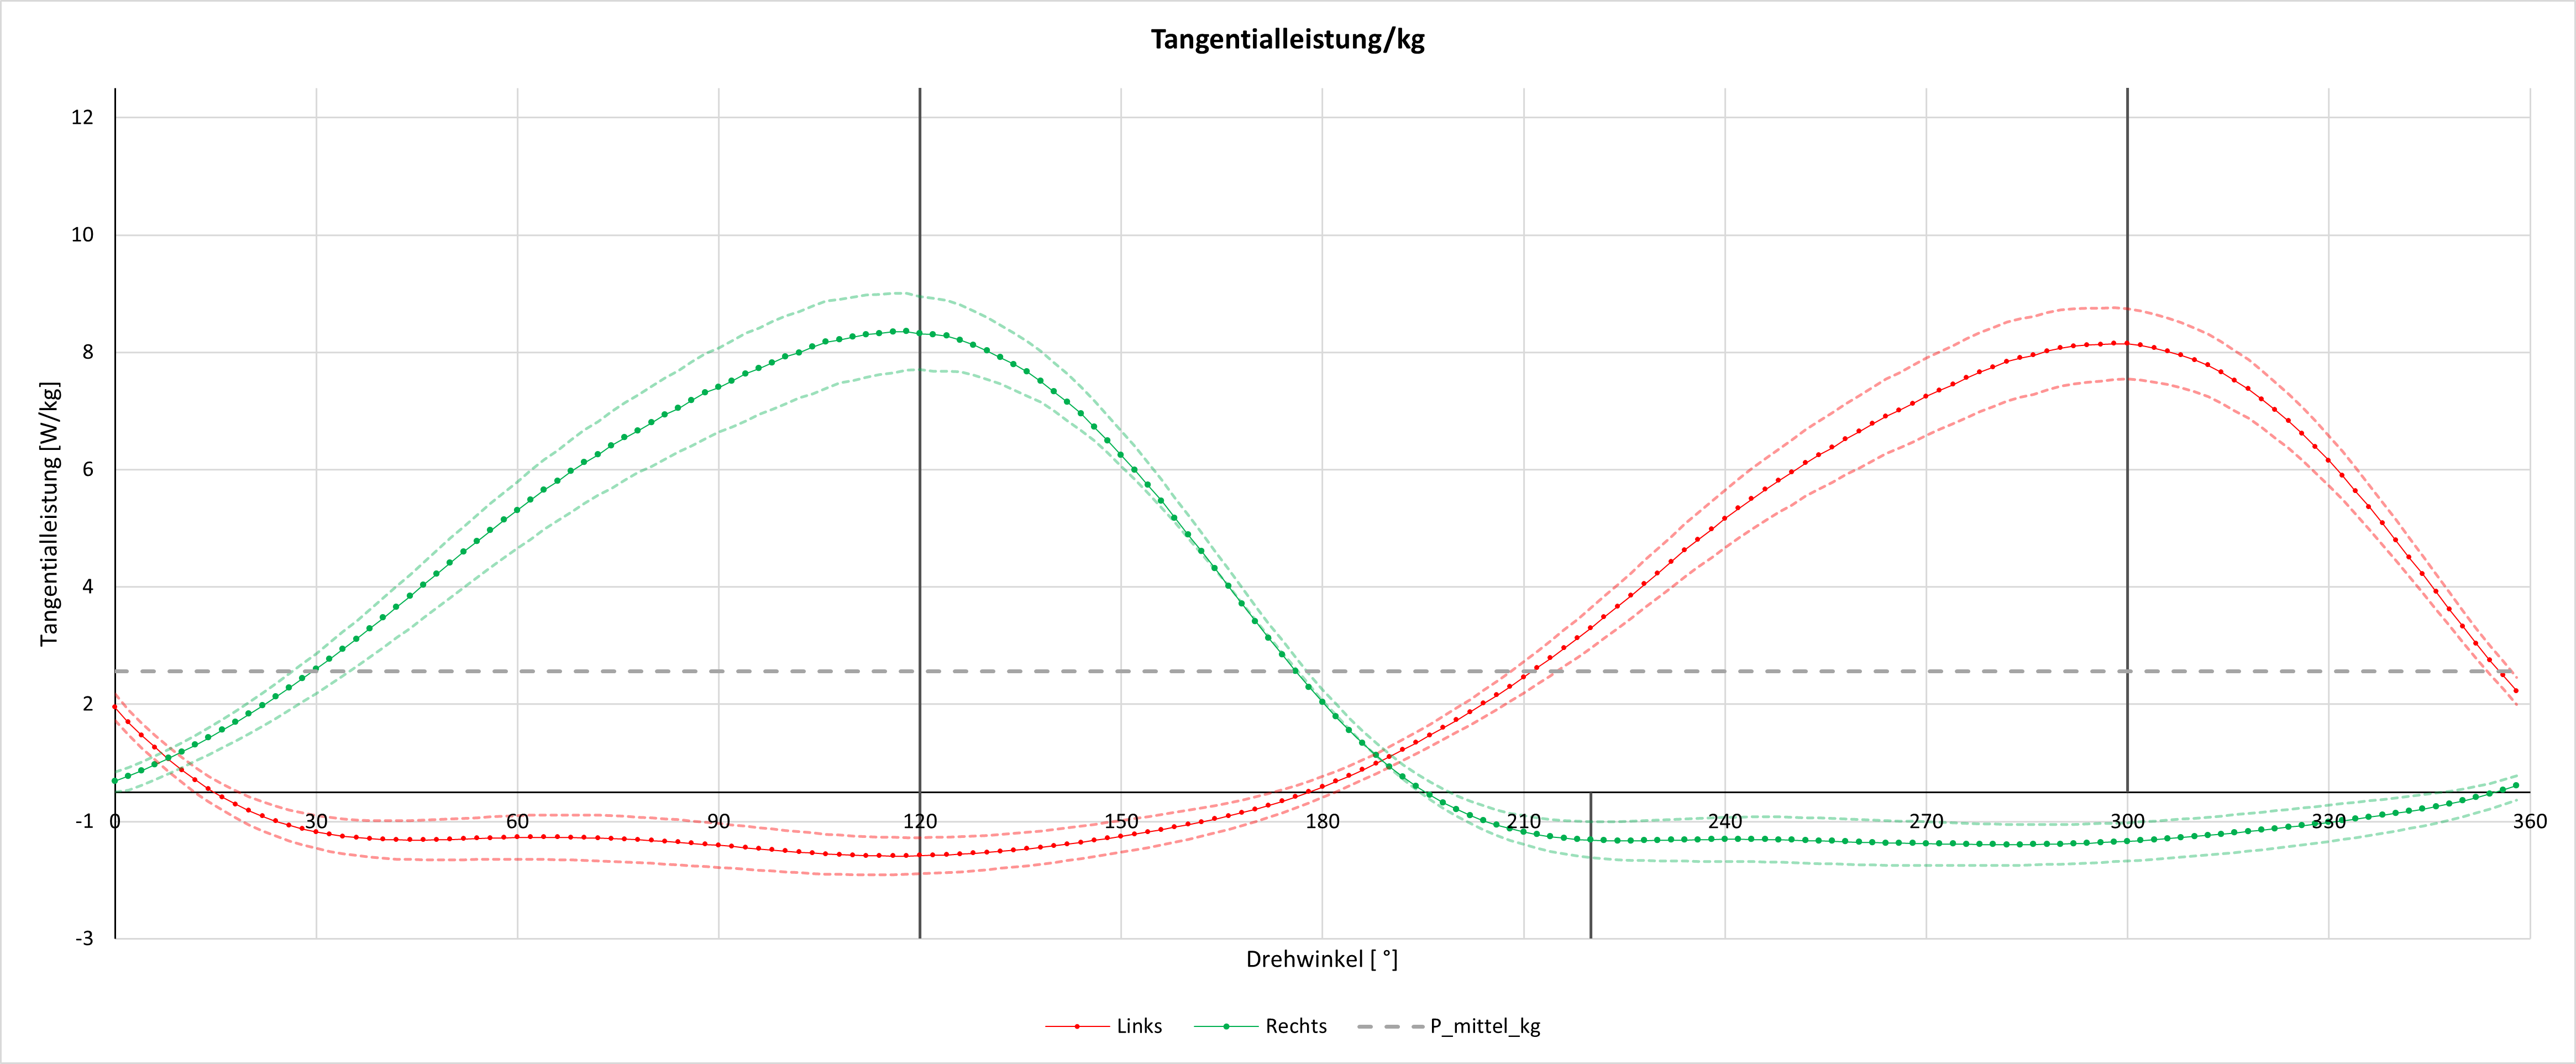
\includegraphics{images/P_komplett.png}

}

\caption{\label{fig-Tangentialleistung_Alle}Verlauf der
gewichtsbezogenen Tangentialleistung aller Durchgänge über den
Drehwinkel für beide Beine}

\end{figure}%

\subsubsection{Leicht\_Sitzen}

\begin{figure}

\centering{

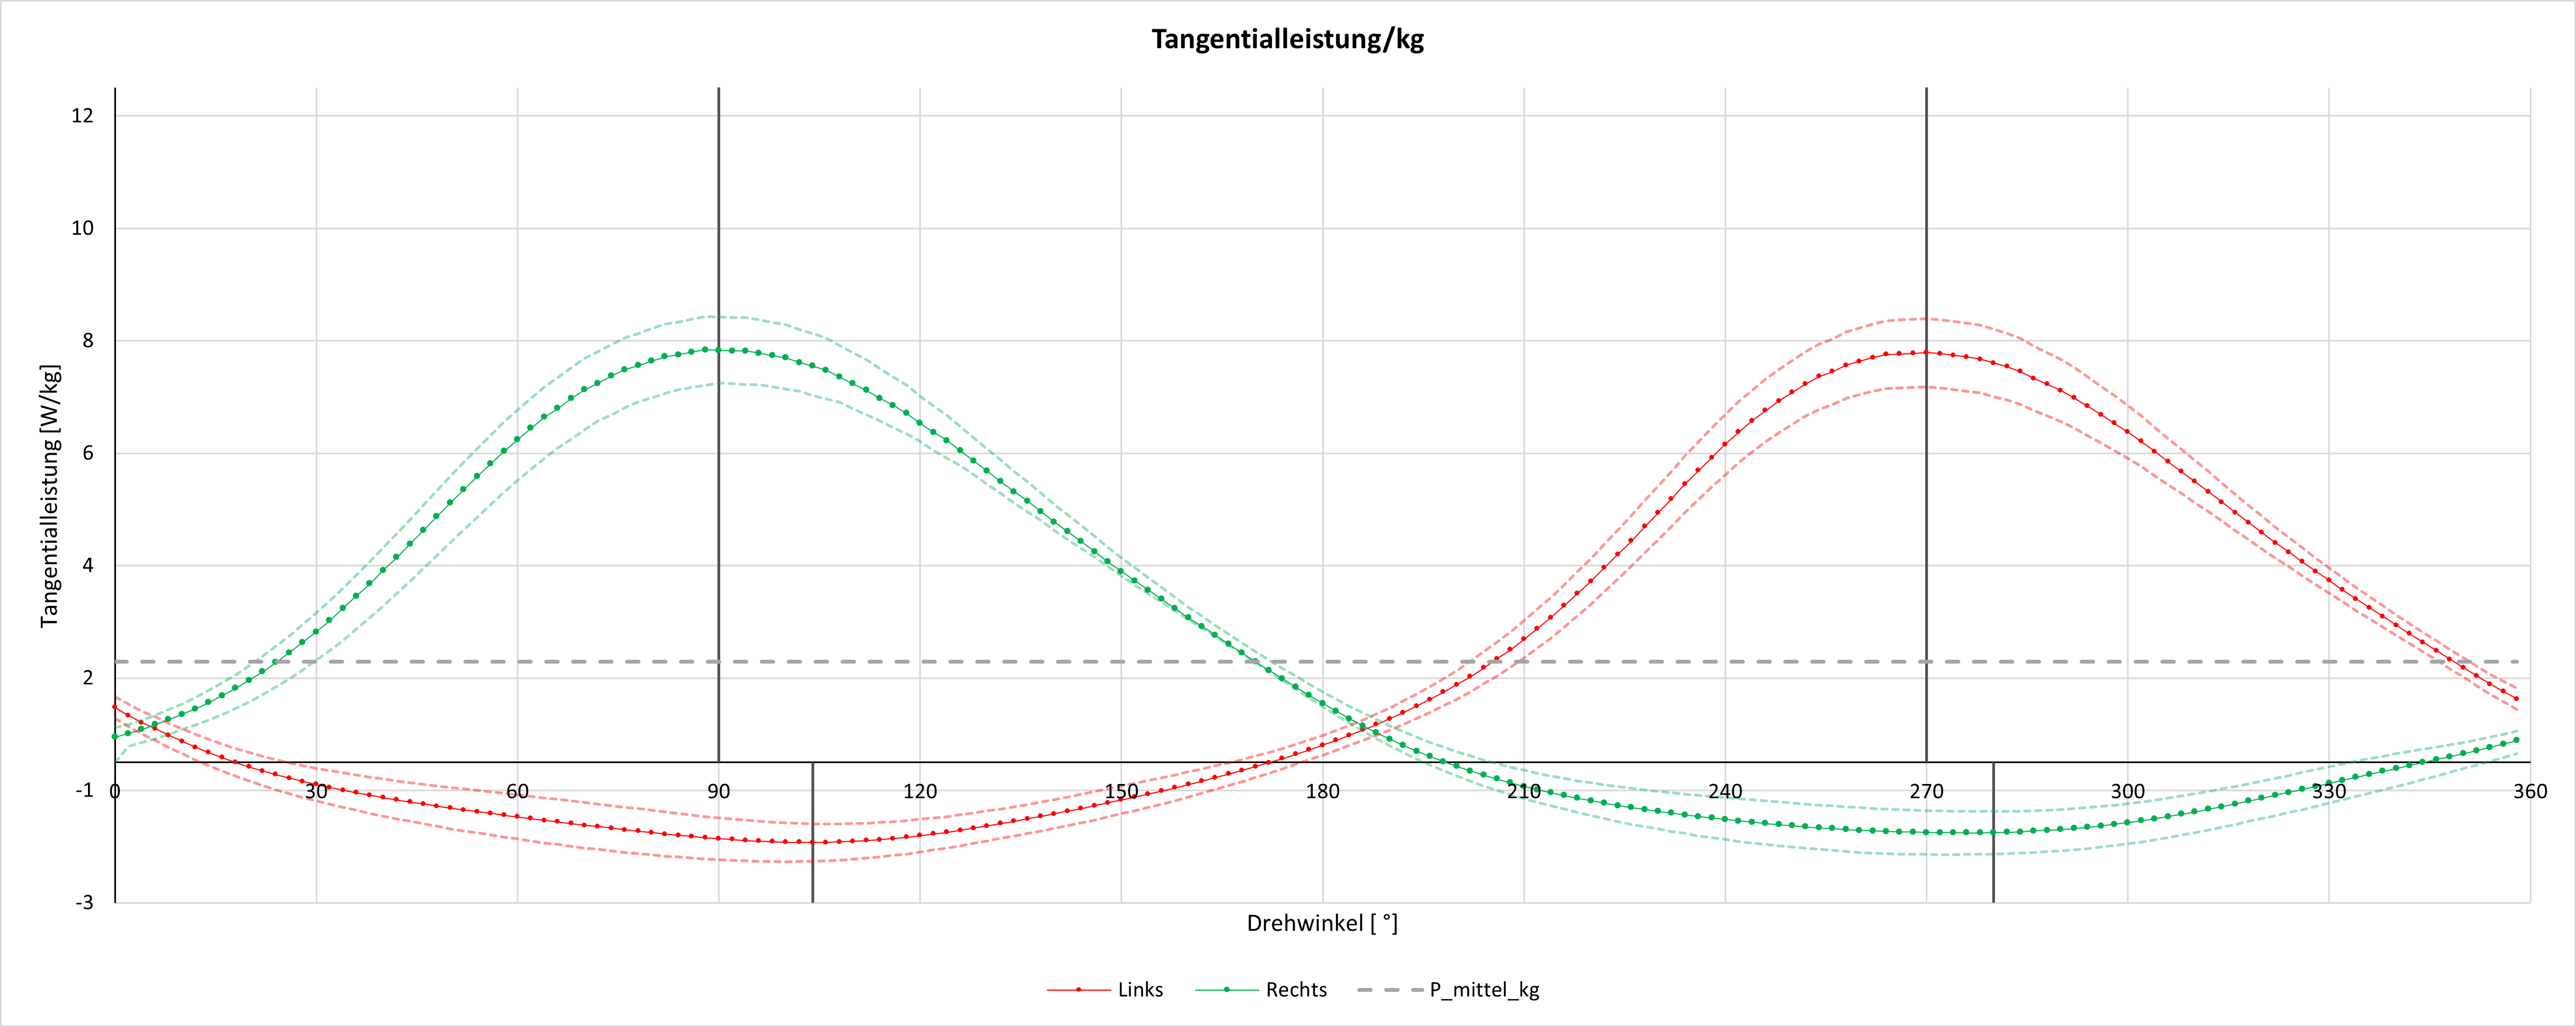
\includegraphics{images/P_leicht_sitzen.png}

}

\caption{\label{fig-Tangentialleistung_Leicht_Sitzen}Verlauf der
gewichtsbezogenen Tangentialleistung der leicht\_sitzen-Bedingung über
den Drehwinkel für beide Beine}

\end{figure}%

\subsubsection{Leicht\_Stehen}

\begin{figure}

\centering{

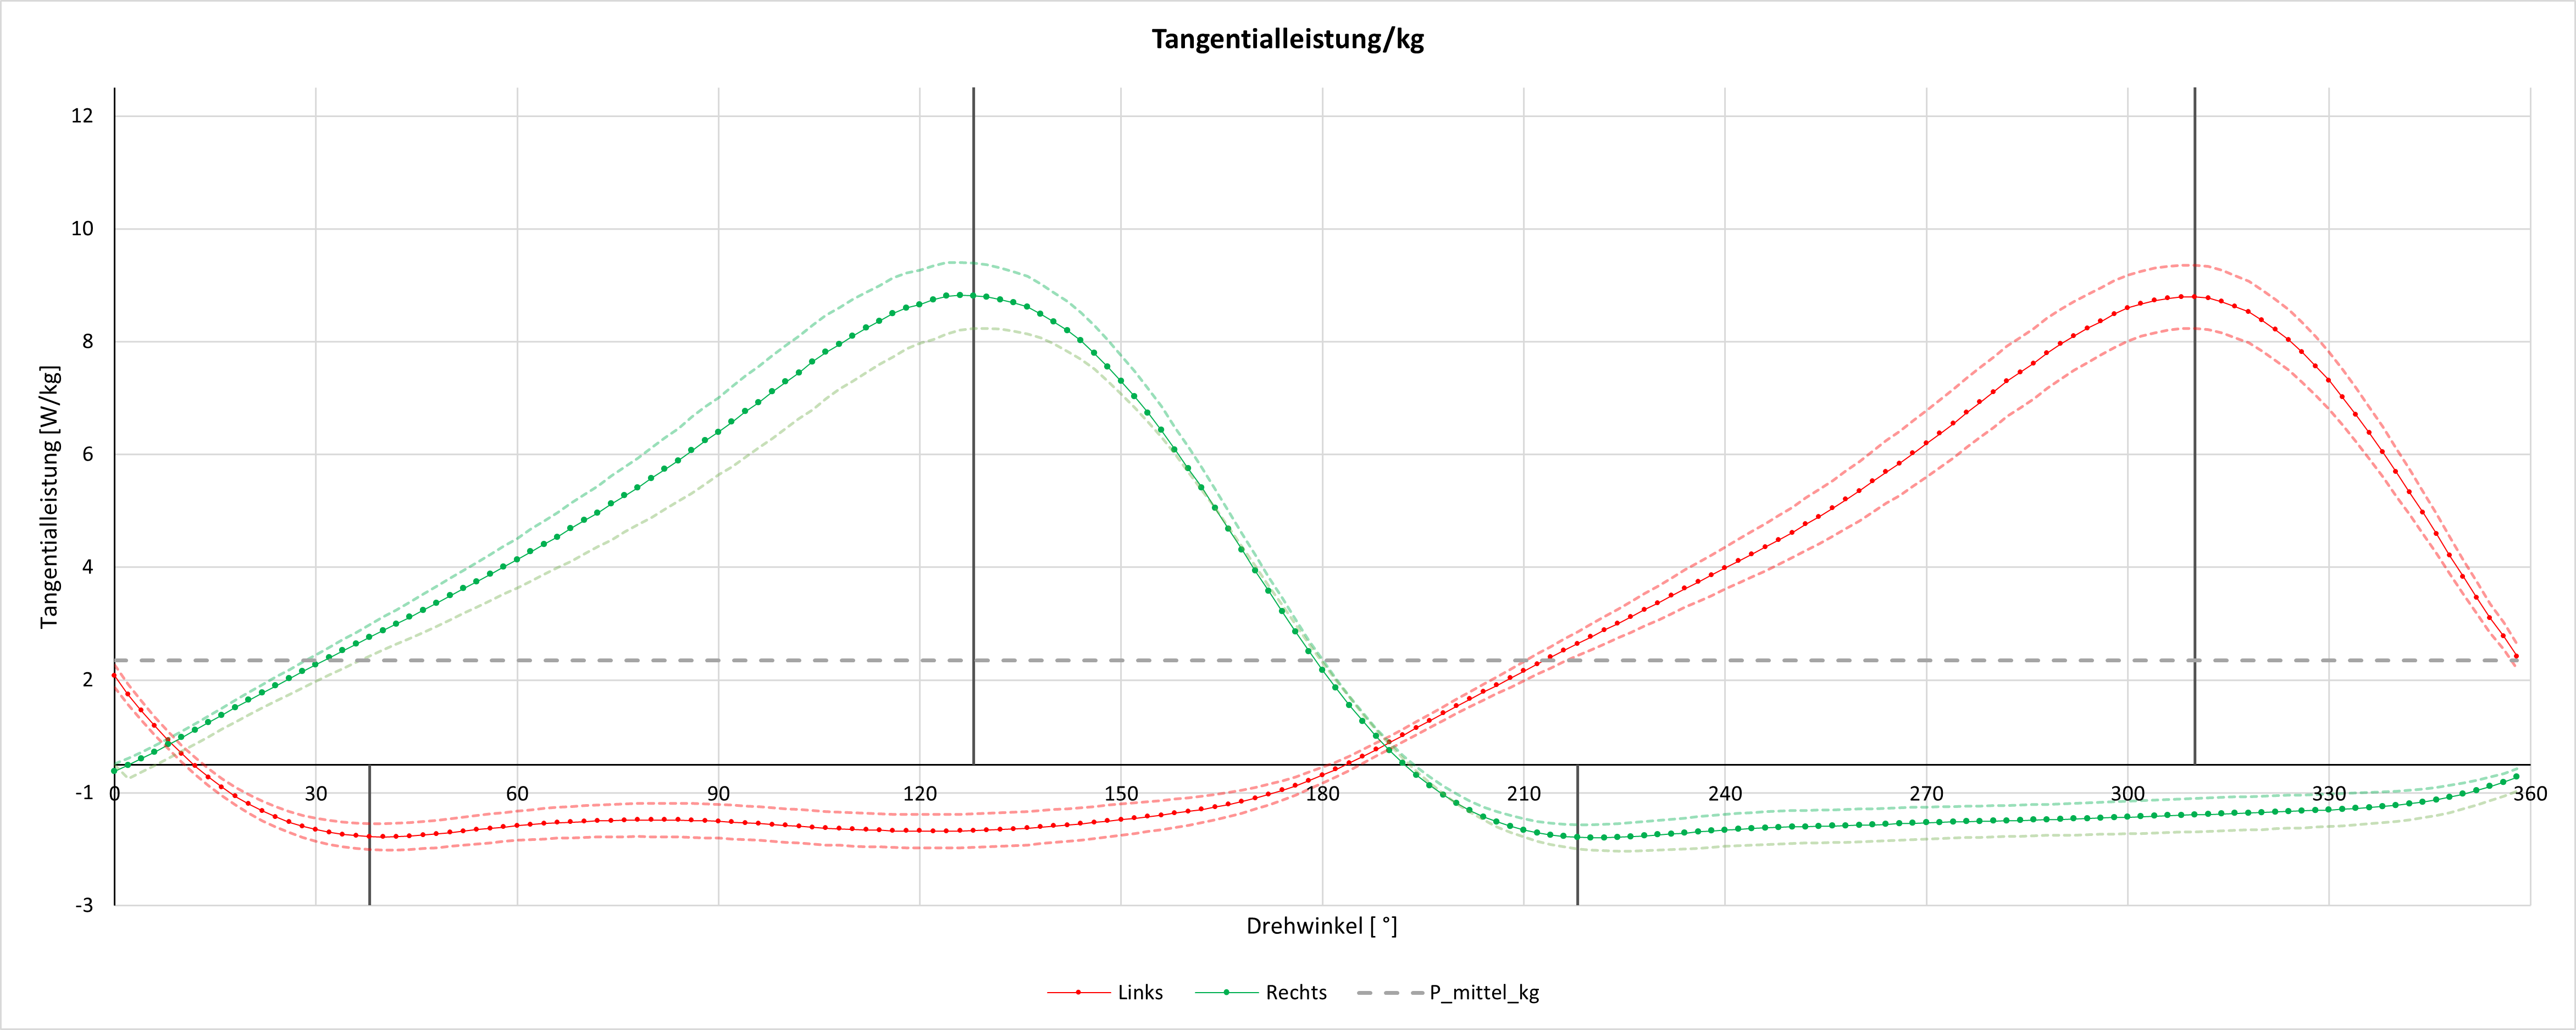
\includegraphics{images/P_leicht_stehen.png}

}

\caption{\label{fig-Tangentialleistung_Leicht_Stehen}Verlauf der
gewichtsbezogenen Tangentialleistung der leicht\_stehen-Bedingung über
den Drehwinkel für beide Beine}

\end{figure}%

\subsubsection{Moderat\_Sitzen}

\begin{figure}

\centering{

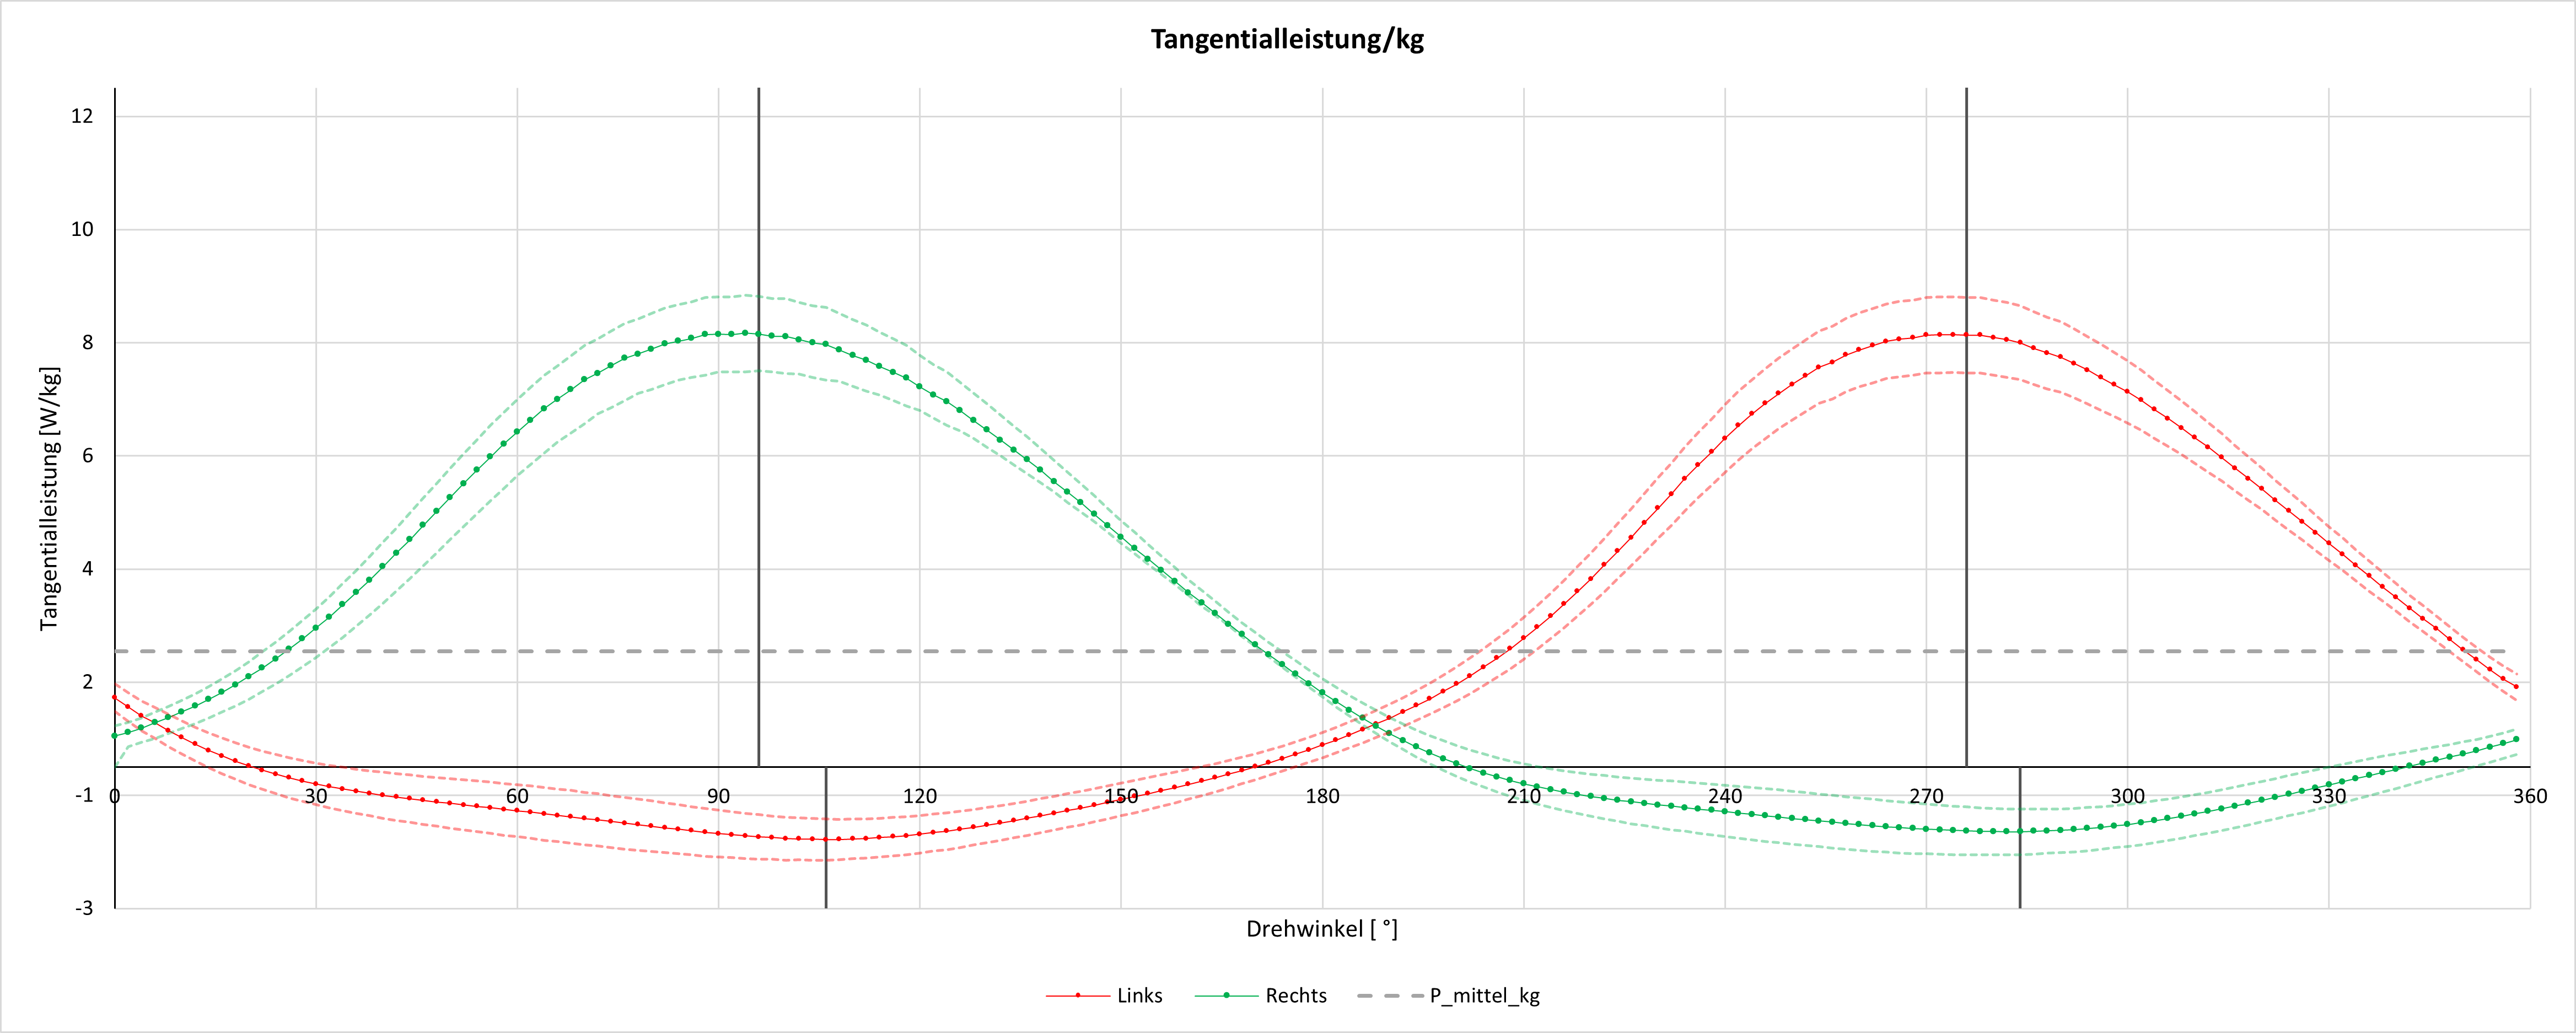
\includegraphics{images/P_moderat_sitzen.png}

}

\caption{\label{fig-Tangentialleistung_Moderat_Sitzen}Verlauf der
gewichtsbezogenen Tangentialleistung der moderat\_sitzen-Bedingung über
den Drehwinkel für beide Beine}

\end{figure}%

\subsubsection{Moderat\_Stehen}

\begin{figure}

\centering{

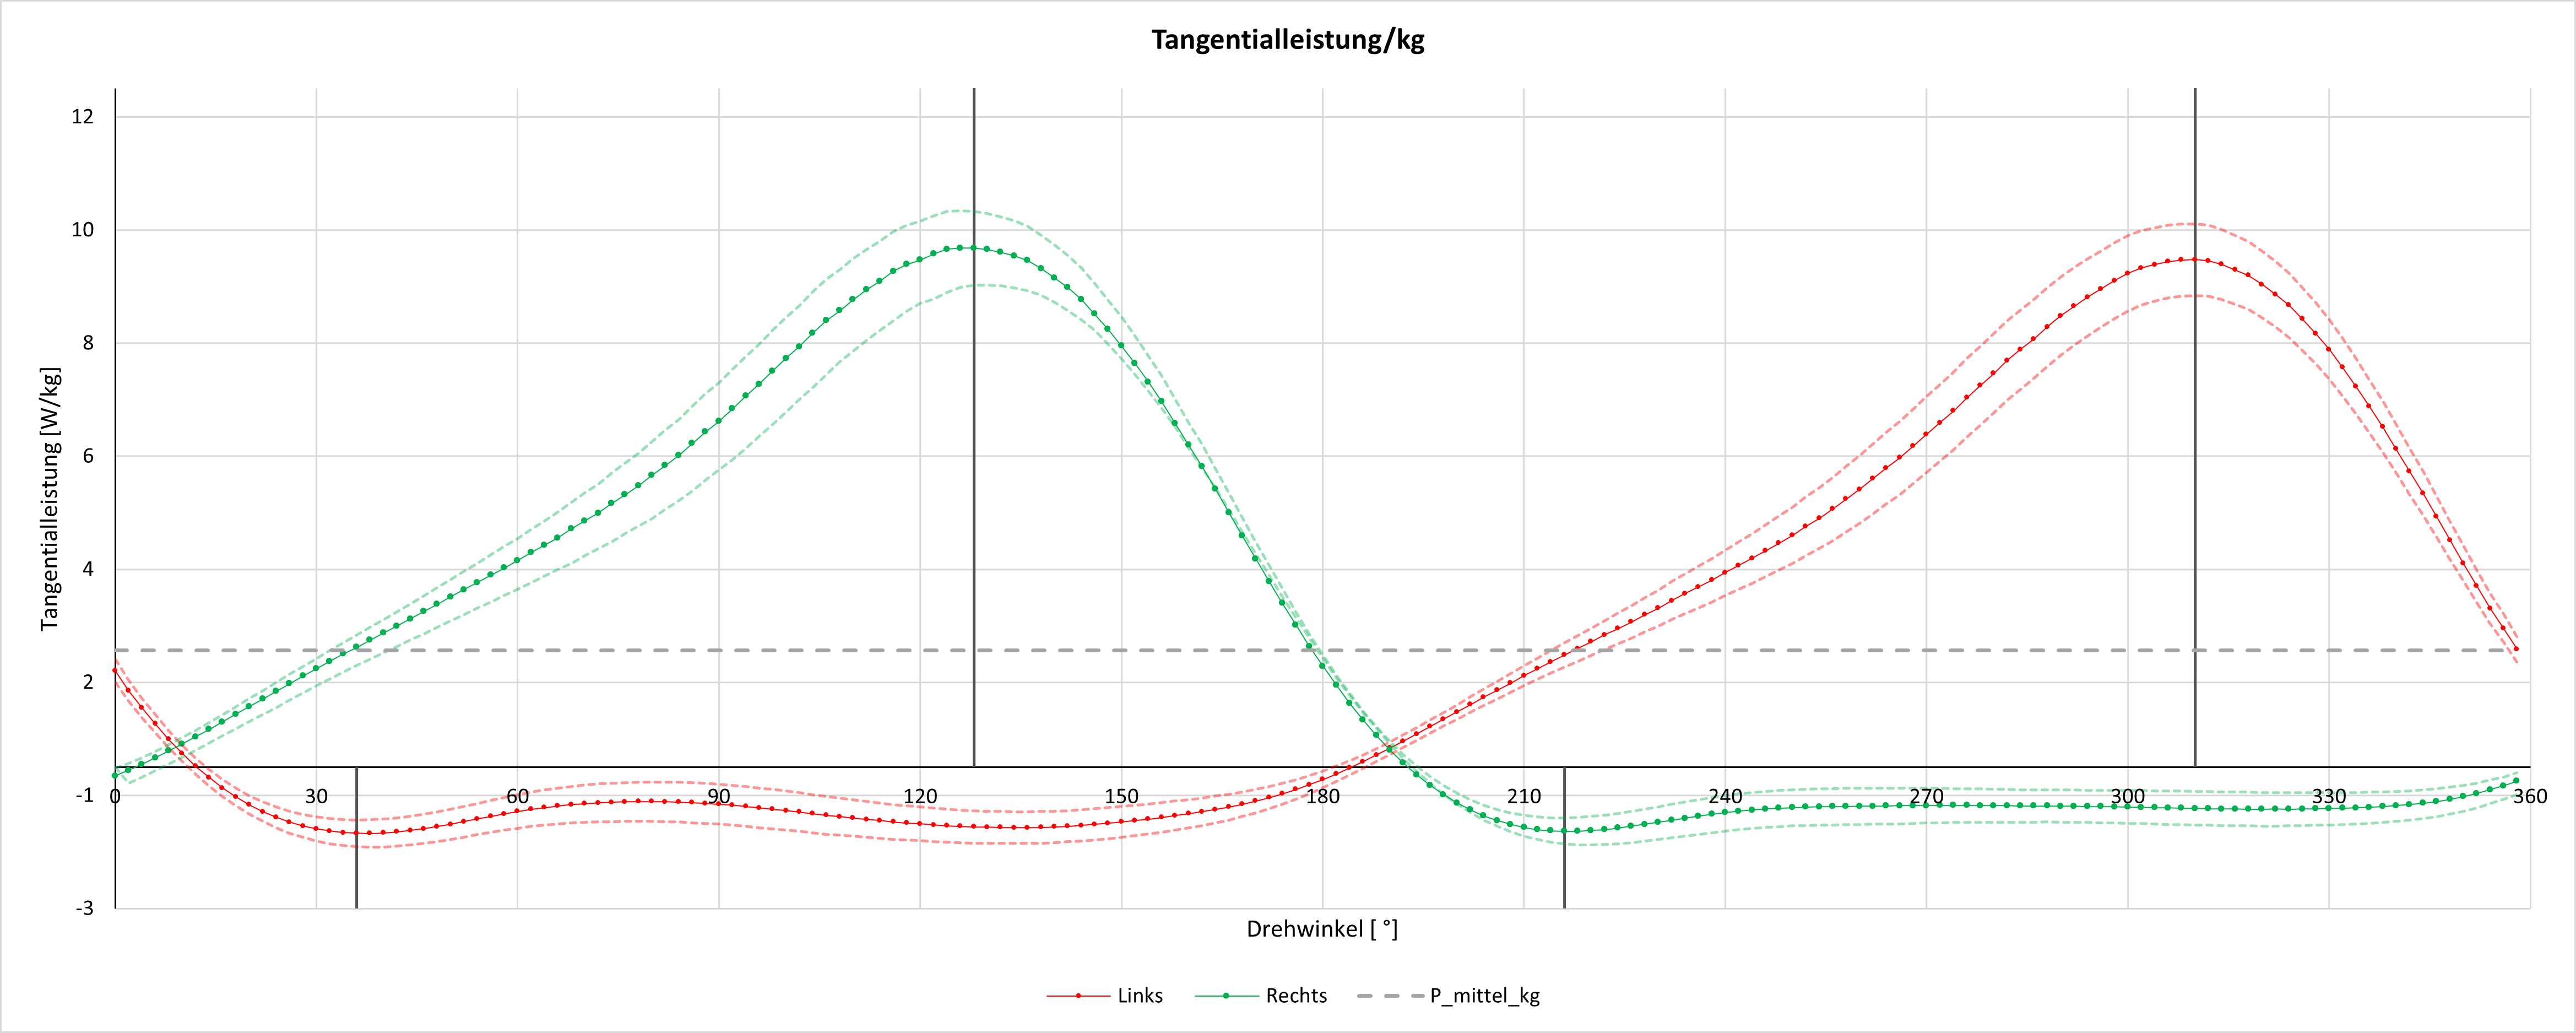
\includegraphics{images/P_moderat_stehen.png}

}

\caption{\label{fig-Tangentialleistung_Moderat_Stehen}Verlauf der
gewichtsbezogenen Tangentialleistung der moderat\_stehen-Bedingung über
den Drehwinkel für beide Beine}

\end{figure}%

\subsubsection{Schwer\_Sitzen}

\begin{figure}

\centering{

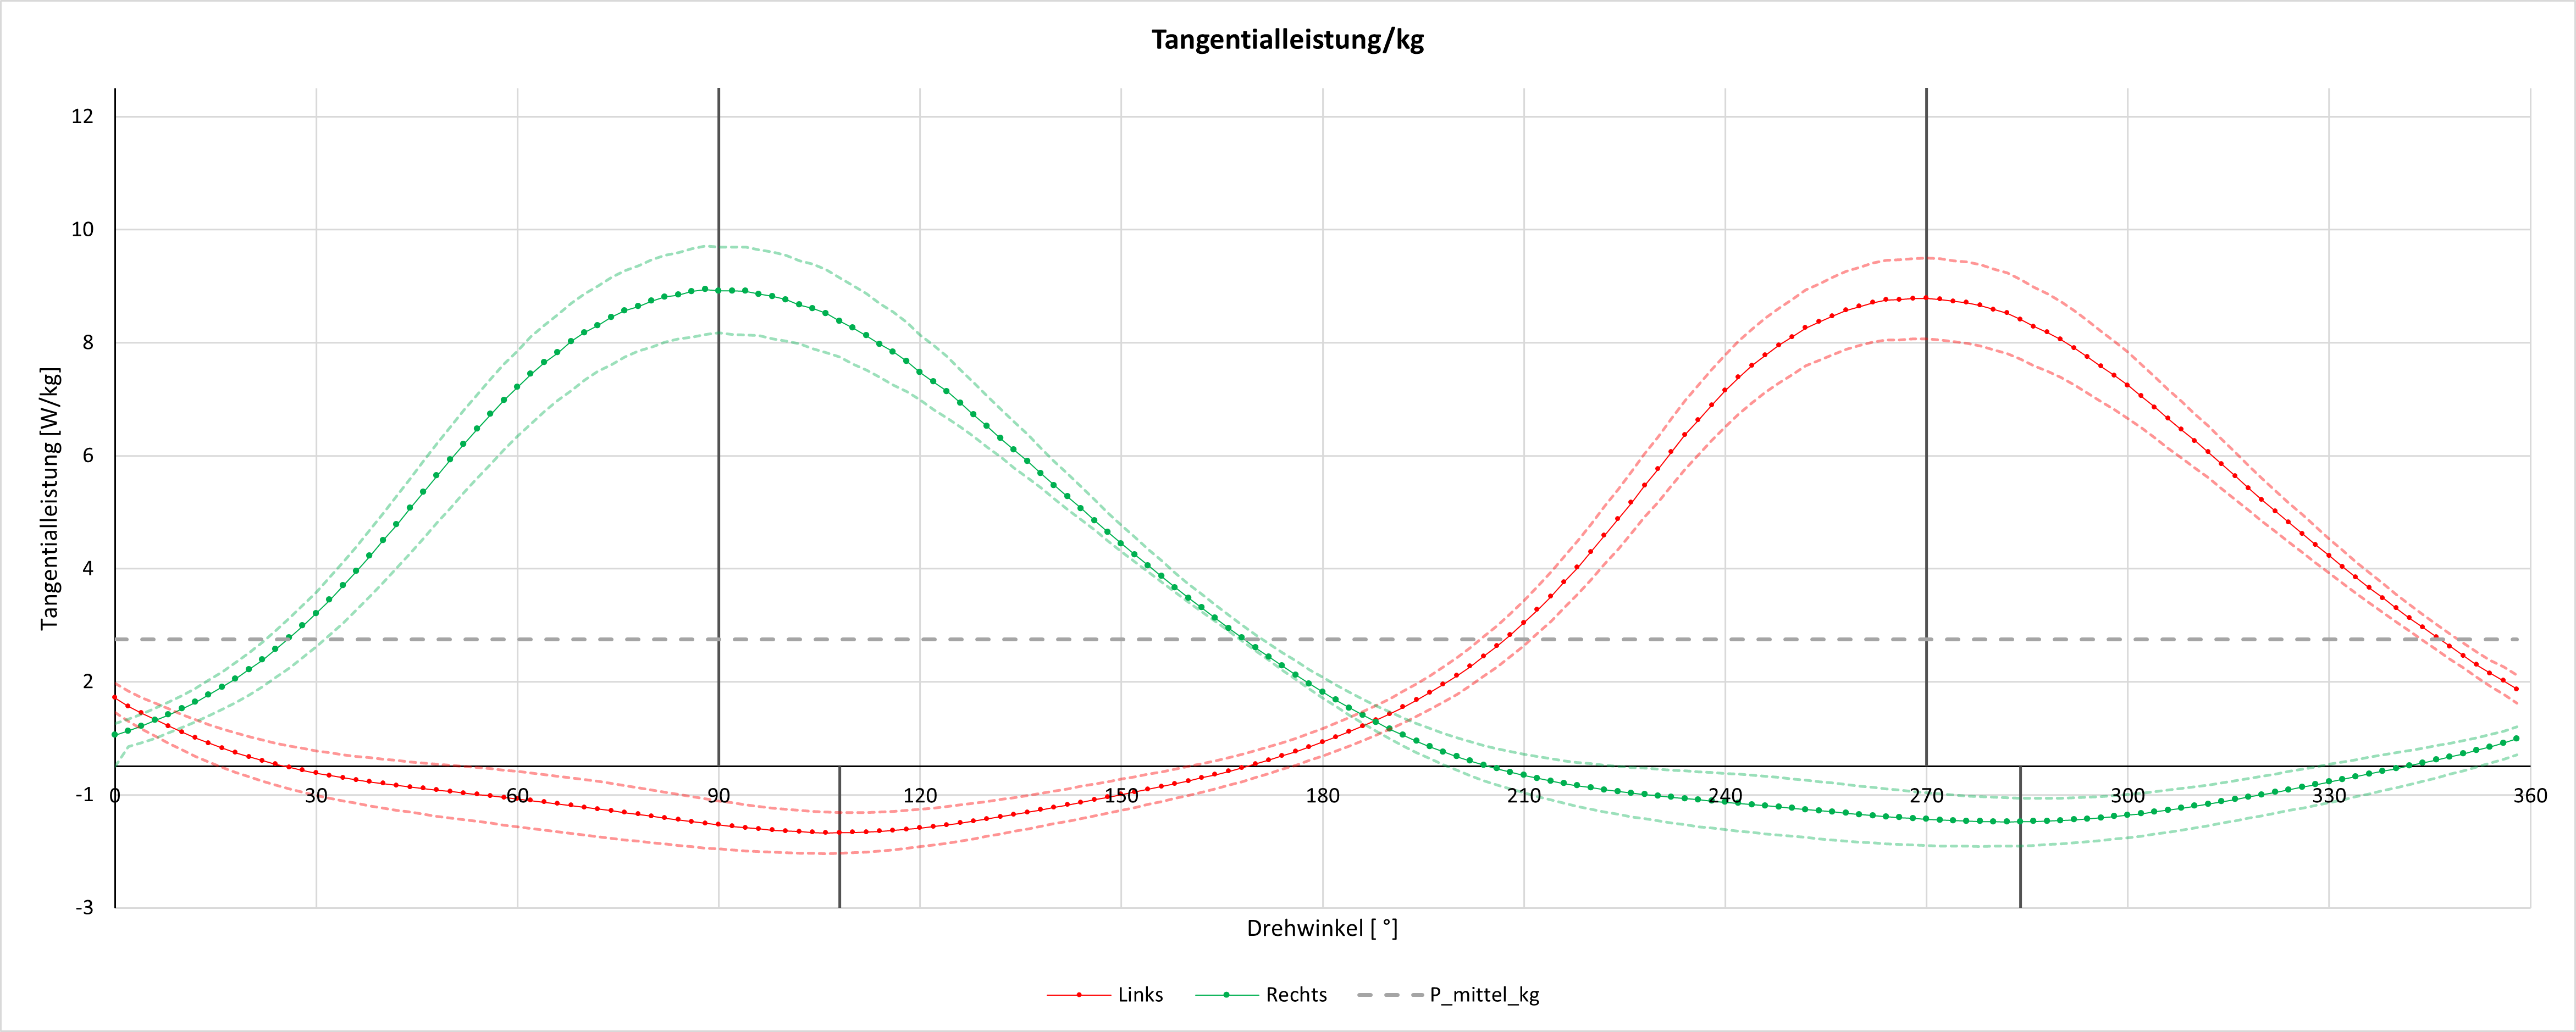
\includegraphics{images/P_schwer_sitzen.png}

}

\caption{\label{fig-Tangentialleistung_Schwer_Sitzen}Verlauf der
gewichtsbezogenen Tangentialleistung der schwer\_sitzen-Bedingung über
den Drehwinkel für beide Beine}

\end{figure}%

\subsubsection{Schwer\_Stehen}

\begin{figure}

\centering{

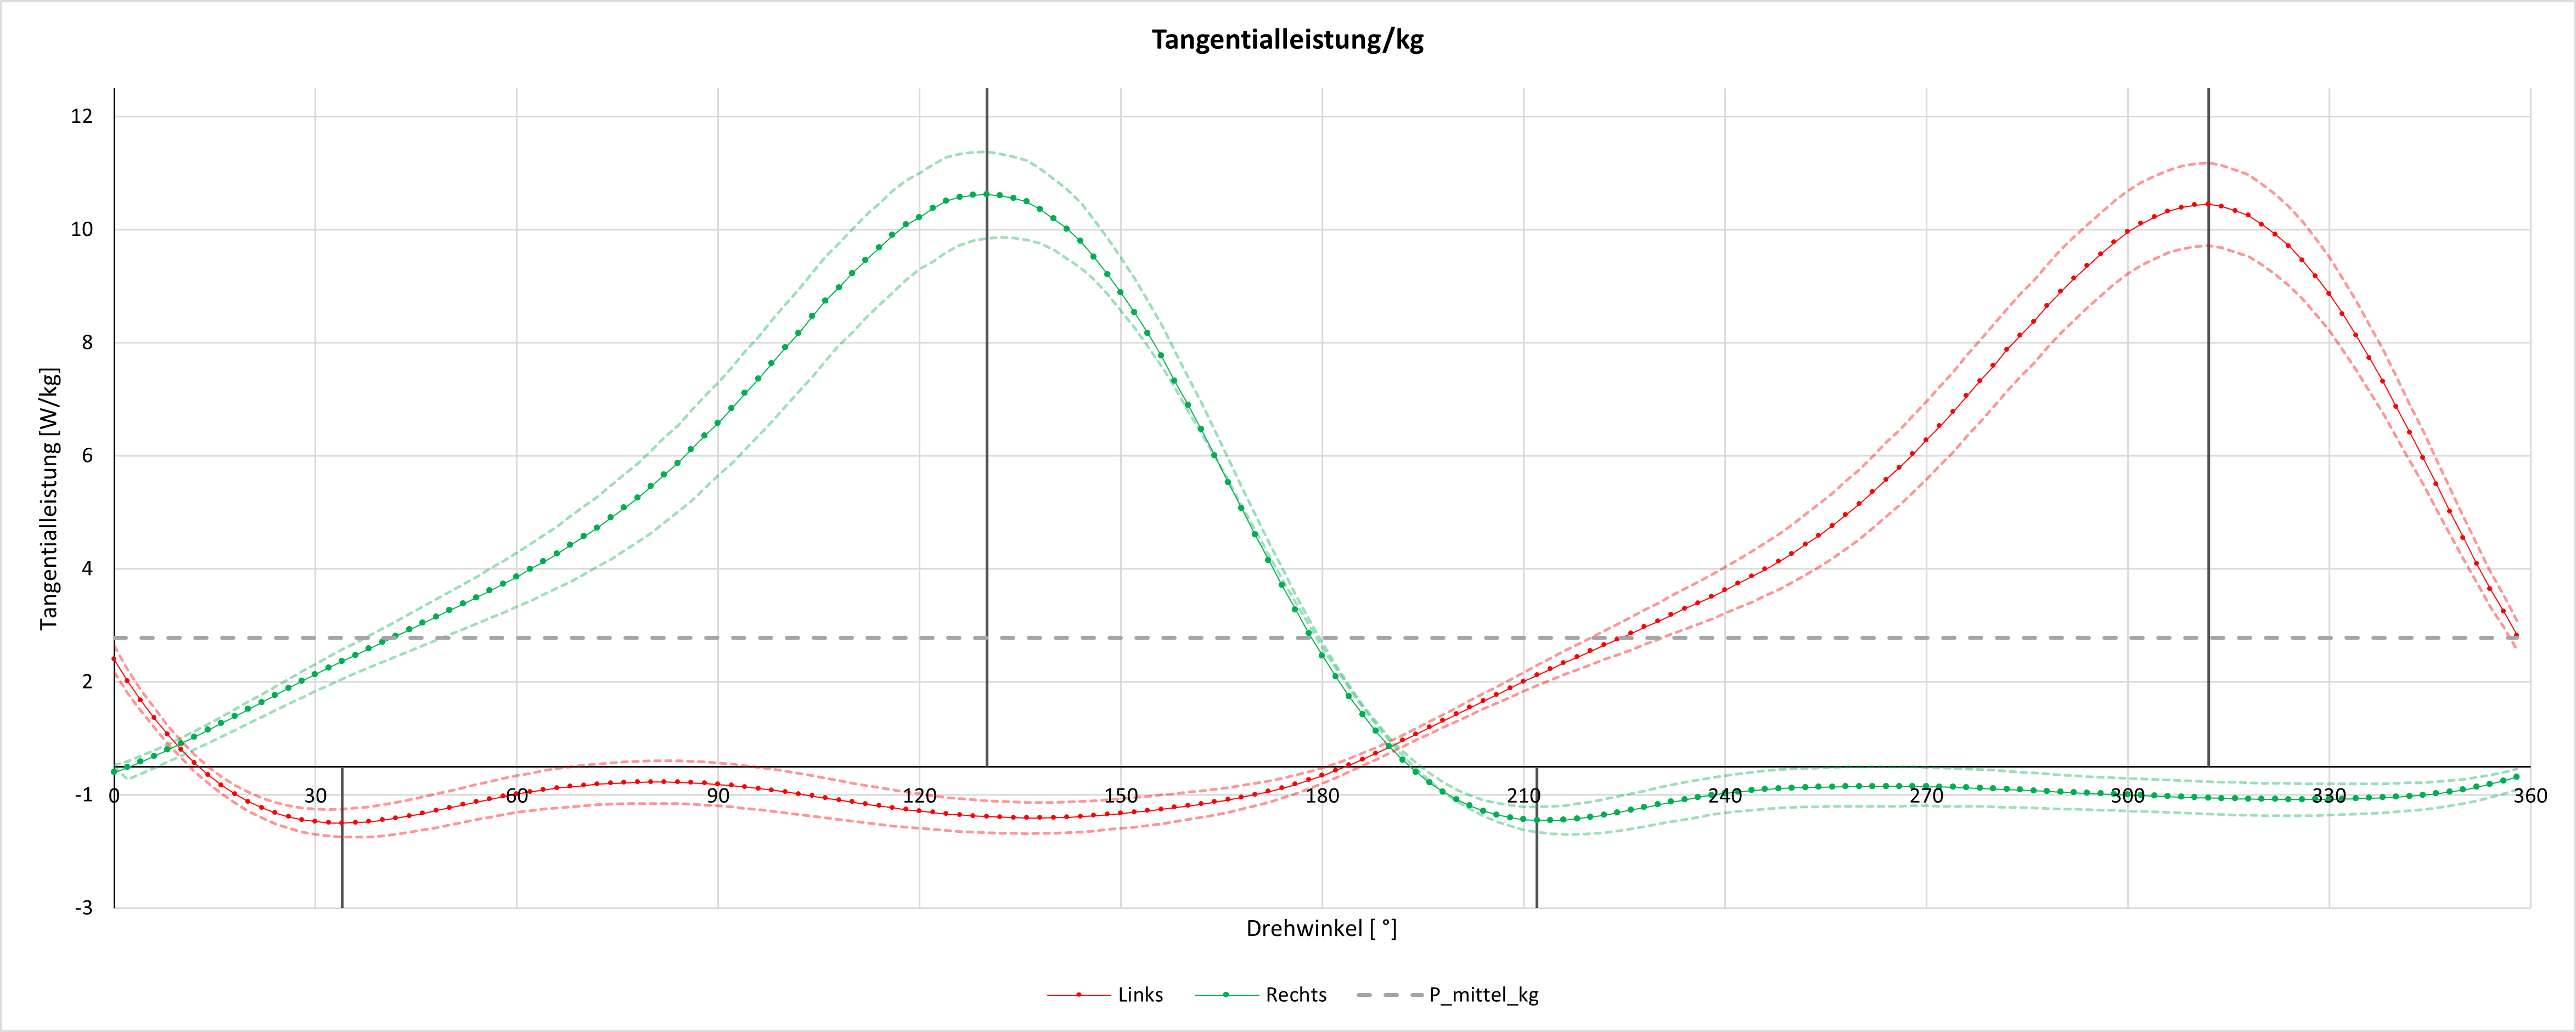
\includegraphics{images/P_schwer_stehen.png}

}

\caption{\label{fig-Tangentialleistung_Schwer_Stehen}Verlauf der
gewichtsbezogenen Tangentialleistung der schwer\_stehen-Bedingung über
den Drehwinkel für beide Beine}

\end{figure}%

\subsection{Kreisförmige Darstellung der positiven und negativen
Leistungsanteile der
Pedalzyklen}\label{kreisfuxf6rmige-darstellung-der-positiven-und-negativen-leistungsanteile-der-pedalzyklen}

Die dargestellten Abbildungen stellen die mittlere Torque Efficiency
sowie die positiven (P+) und negativen (P-) Leistungsanteile während der
Pedalzyklen kreisförmig dar. Im Vergleich der Fahrbedingungen zeigt sich
im Sitzen eine leicht höhere durchschnittliche Torque Efficiency
(78.17\%) als im Stehen (76.43\%)
(Abbildung~\ref{fig-Eff_KD_Bedingung}). Mit steigender Intensität steigt
die Torque Efficiency von 71.17\% (leicht) über 77.86\% (moderat) auf
82.87\% (schwer) (Abbildung~\ref{fig-Eff_KD_Intensität}). Diese
Steigerung ist in beiden Fahrbedingungen zu beobachten, wobei im Stehen
bei leichter Intensität die geringste (69.19\%) und bei schwerer
Intensität die höchste Torque Efficiency (83.04\%) erreicht wird
(Abbildung~\ref{fig-Eff_KD_Bedingung_Intensität}). Die positiven
Leistungsanteile (grün) und negativen Leistungsanteile (rot) bleiben
innerhalb den Bedingungen über die Kurbelumdrehung weitgehend konstant.

\subsubsection{Bedingungen}

\begin{figure}

\centering{

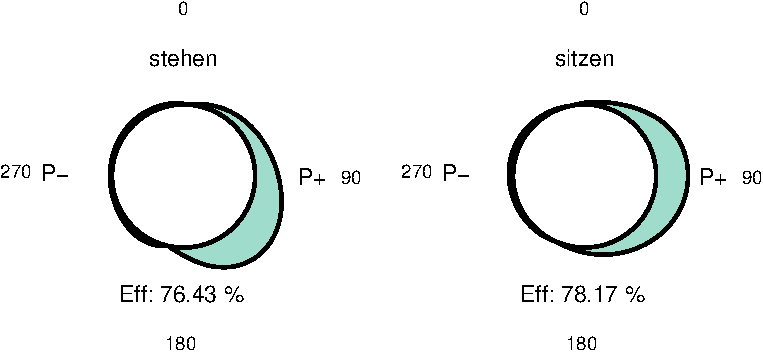
\includegraphics{Ergometer_Daten_files/figure-pdf/fig-Eff_KD_Bedingung-1.pdf}

}

\caption{\label{fig-Eff_KD_Bedingung}Kreisförmige Darstellung der
mittleren positiven (P+) und negativen (P-) Leistungsanteile mit
resultierender Torque Efficiency während der Pedalzyklen in stehender
und sitzender Position}

\end{figure}%

\subsubsection{Intensitäten}

\begin{figure}

\centering{

\includegraphics{Ergometer_Daten_files/figure-pdf/fig-Eff_KD_Intensität-1.pdf}

}

\caption{\label{fig-Eff_KD_Intensität}Kreisförmige Darstellung der
mittleren positiven (P+) und negativen (P-) Leistungsanteile mit
resultierender Torque Efficiency während der Pedalzyklen in den drei
Intensitätsstufen}

\end{figure}%

\subsubsection{Bedingungen\_Intensitäten}

\begin{figure}

\centering{

\includegraphics{Ergometer_Daten_files/figure-pdf/fig-Eff_KD_Bedingung_Intensität-1.pdf}

}

\caption{\label{fig-Eff_KD_Bedingung_Intensität}Kreisförmige Darstellung
der mittleren positiven (P+) und negativen (P-) Leistungsanteile mit
resultierender Torque Efficiency während der Pedalzyklen in den
Bedingungen sowie drei Intensitätsstufen}

\end{figure}%

\subsection{Zusammenhänge von Effizienzparametern der Tretbewegung und
mechanischer
Leistung}\label{zusammenhuxe4nge-von-effizienzparametern-der-tretbewegung-und-mechanischer-leistung}

Die nachstehenden Abbildungen zeigen die Zusammenhänge zwischen
verschiedenen biomechanischen Parametern der Tretbewegung beim
Radfahren. Die erste Analyse untersucht die Beziehung zwischen
P\textsubscript{mech,kg} und der Torque Efficiency und zeigt einen
starken, signifikanten Zusammenhang (F\textsubscript{(1,52)} = 112.80, p
\textless{} .001, R² = 0.68). Dies deutet darauf hin, dass Probanden mit
höheren P\textsubscript{mech,kg} Werten in der letzten Stufe des
Stufentests tendenziell auch höhere Torque Efficiency Werte aufweisen.
Für die Pedal Smoothness zeigt sich ebenfalls ein signifikanter, wenn
auch moderaterer Zusammenhang mit P\textsubscript{mech,kg}
(F\textsubscript{(1,52)} = 28.56, p \textless{} .001, R² = 0.35). Die
Daten legen nahe, dass leistungsstärkere Probanden möglicherweise eine
gleichmäßigere Trittbewegung mit geringeren relativen Leistungsspitzen
im Pedalzyklus aufweisen könnten. Der hochsignifikante positive
Zusammenhang zwischen Pedal Smoothness und Torque Efficiency
(F\textsubscript{(1,52)} = 67.24, p \textless{} .001, R² = 0.56) könnte
auf eine Verbindung dieser Parameter hinweisen. Die Daten deuten an,
dass eine höhere Effizienz der Kraftübertragung mit einer
gleichmäßigeren Tretbewegung einhergehen könnte.

\subsubsection{\texorpdfstring{Torque Efficiency und
P\textsubscript{mech}}{Torque Efficiency und Pmech}}

\begin{figure}

\centering{

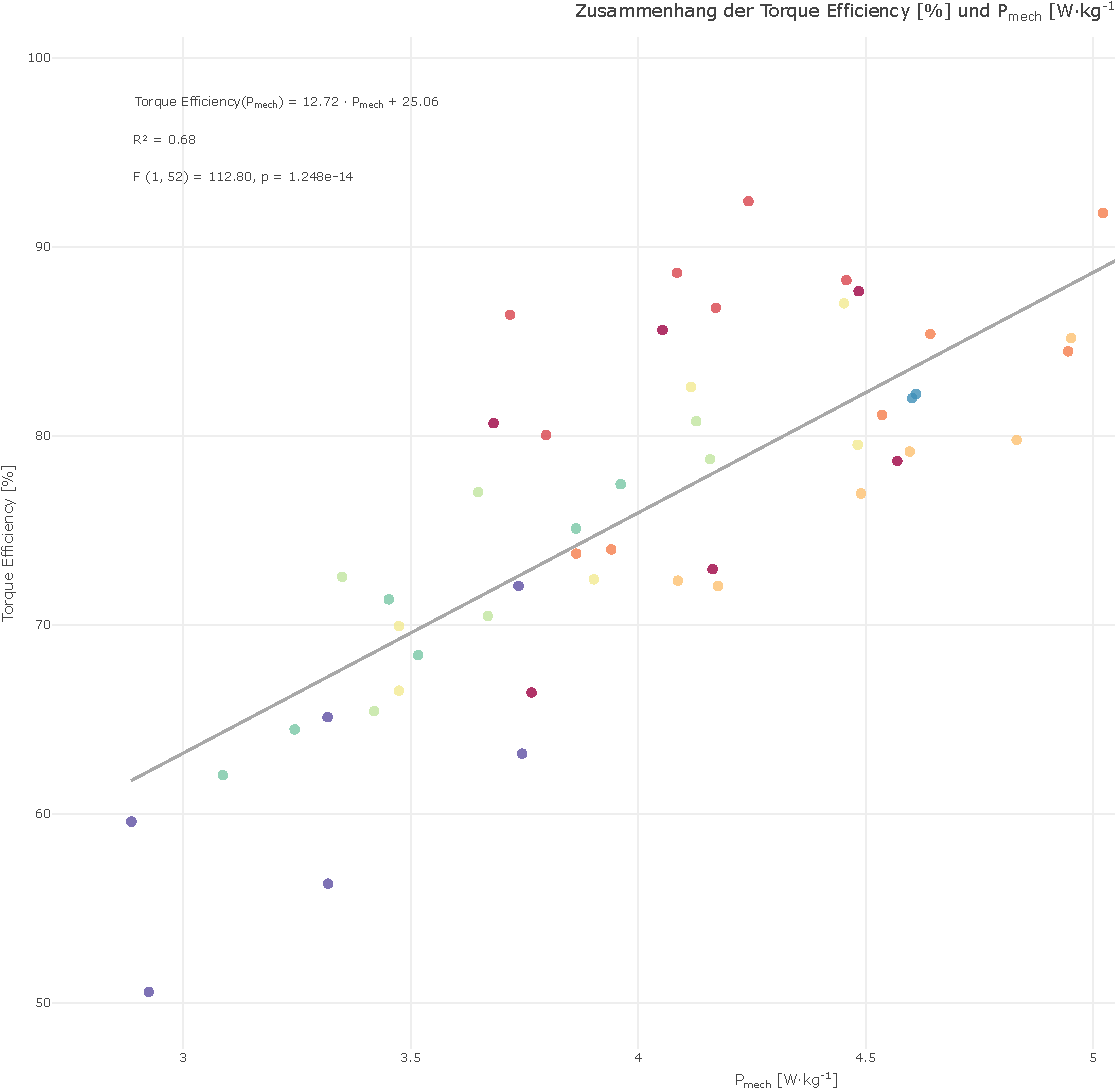
\includegraphics{Ergometer_Daten_files/figure-pdf/fig-TE_P_mech-1.pdf}

}

\caption{\label{fig-TE_P_mech}Zusammenhang der Torque Efficiency
{[}\%{]} und Pmech {[}W·kg-1{]}}

\end{figure}%

\subsubsection{\texorpdfstring{Pedal Smoothness und
P\textsubscript{mech}}{Pedal Smoothness und Pmech}}

\begin{figure}

\centering{

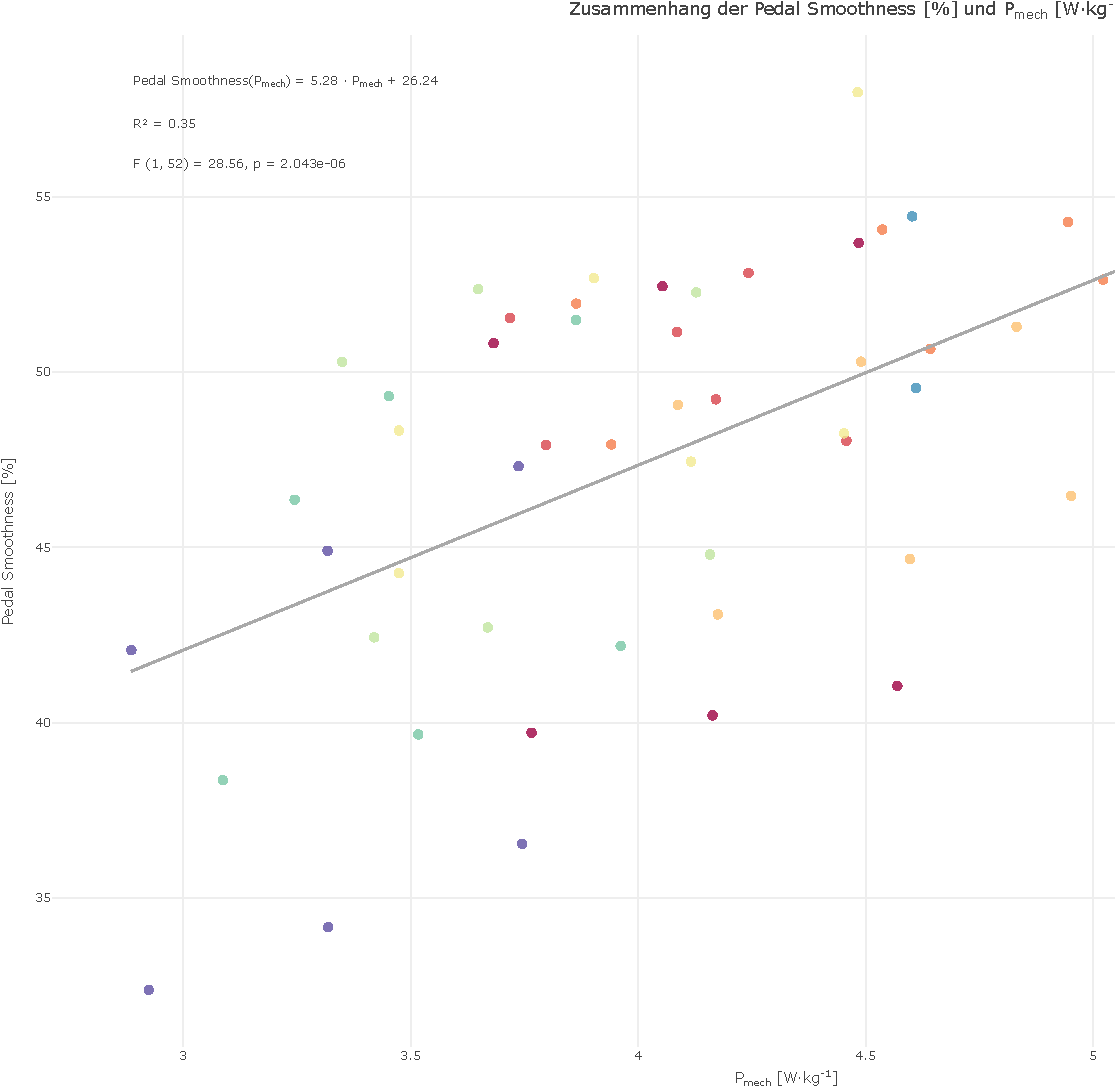
\includegraphics{Ergometer_Daten_files/figure-pdf/fig-PS_P_mech-1.pdf}

}

\caption{\label{fig-PS_P_mech}Zusammenhang der Pedal Smoothness {[}\%{]}
und Pmech {[}W·kg-1{]}}

\end{figure}%

\subsubsection{Pedal Smoothness und Torque Efficiency}

\begin{figure}

\centering{

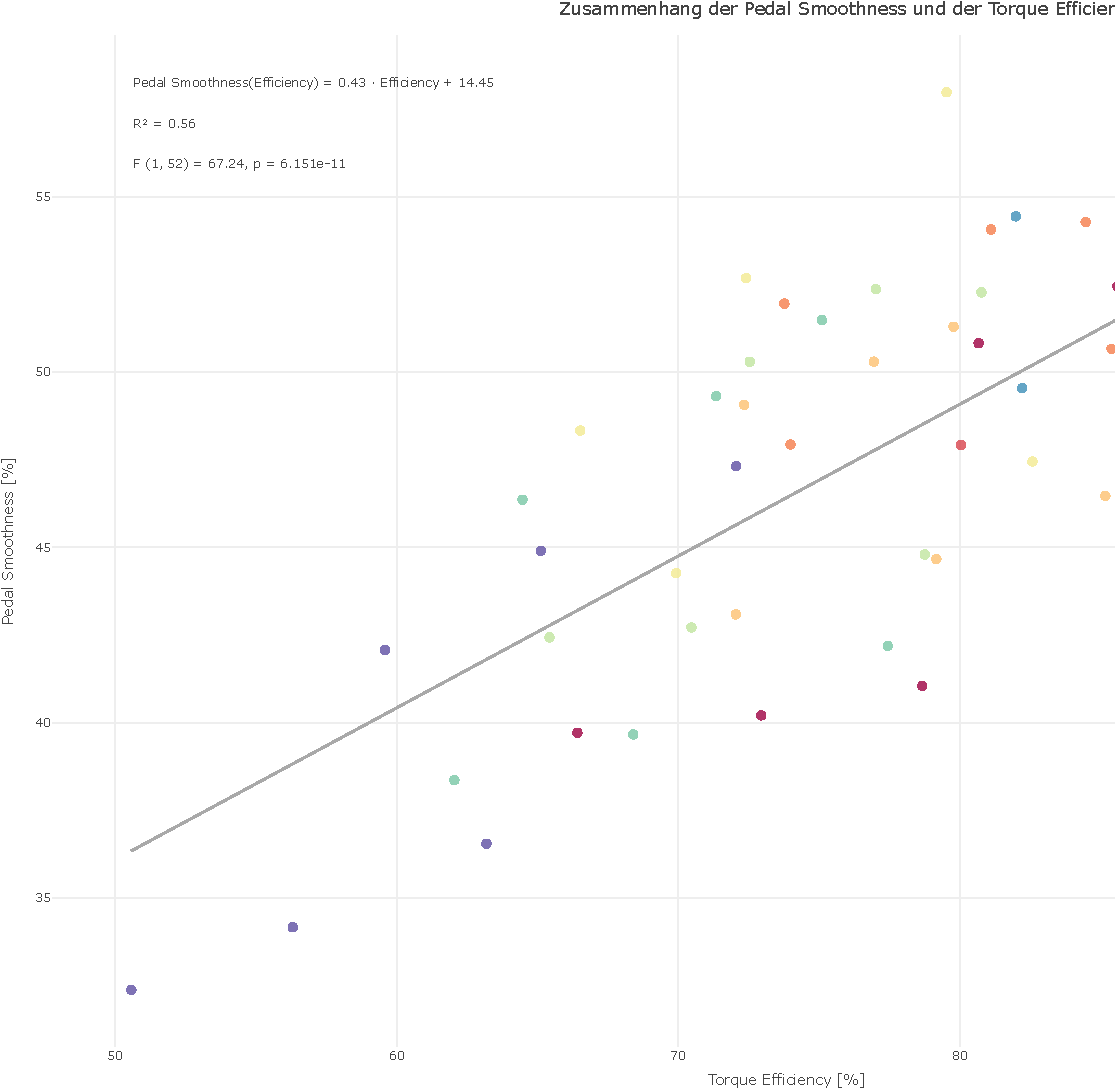
\includegraphics{Ergometer_Daten_files/figure-pdf/fig-TE_PS-1.pdf}

}

\caption{\label{fig-TE_PS}Zusammenhang der Pedal Smoothness und der
Torque Efficiency}

\end{figure}%

\subsection{Interaktive Analyse der Zusammenhänge ausgewählter
verschiedener Leistungsparameter mittels linearer
Regression}\label{interaktive-analyse-der-zusammenhuxe4nge-ausgewuxe4hlter-verschiedener-leistungsparameter-mittels-linearer-regression}

Die folgende Shiny-App bietet die Möglichkeit zur Analyse von weiteren
Zusammenhängen ausgewählter Leistungsparameter. In der Seitenleiste
können die ausgewählten Daten nach Probanden, Intensitäten und
Bedingungen gefiltert werden. Die Auswahl der x- und y-Achse definiert
die Variablen für die Regressionsanalyse. Es wird ein interaktives
Streudiagramm mit Regressionslinie erstellt, das den linearen
Zusammenhang der gewählten Parameter darstellt. Die Anwendung analysiert
verschiedene anthropometrische sowie physiologische und ergometrische
Leistungsparameter. Für jede Parameterkombination erfolgt eine lineare
Regressionsanalyse mit Regressionsgleichung, Bestimmtheitsmaß
(R\textsuperscript{2}) und statistischer Signifikanz.

\begin{Shaded}
\begin{Highlighting}[]
\NormalTok{\#| \textquotesingle{}!! shinylive warning !!\textquotesingle{}: |}
\NormalTok{\#|   shinylive does not work in self{-}contained HTML documents.}
\NormalTok{\#|   Please set \textasciigrave{}embed{-}resources: false\textasciigrave{} in your metadata.}
\NormalTok{\#| standalone: true}
\NormalTok{\#| viewerHeight: 650}
\NormalTok{library(shiny)}
\NormalTok{library(plotly)}
\NormalTok{library(dplyr)}
\NormalTok{library(broom)}
\NormalTok{library(RColorBrewer)}
\NormalTok{library(DT)}

\NormalTok{Bedingungen\_data\_Shiny\_Regression \textless{}{-} data.frame(}
\NormalTok{  \textasciigrave{}Proband\textasciigrave{} = c( "01", "01", "01", "01", "01", "01", "06", "06", "06", "06", "06", "06", "10", "10", "10", "10", "10", "10", "13", "13", "13", "13", "13", "13", "15", "15", "15", "15", "15", "15", "19", "19", "19", "19", "19", "19", "20", "20", "20", "20", "20", "20", "22", "22", "22", "22", "22", "22", "23", "23", "23", "23", "23", "23" ),}
\NormalTok{  \textasciigrave{}Nr\textasciigrave{} = c( 1, 2, 3, 4, 5, 6, 1, 2, 3, 4, 5, 6, 1, 2, 3, 4, 5, 6, 1, 2, 3, 4, 5, 6, 1, 2, 3, 4, 5, 6, 1, 2, 3, 4, 5, 6, 1, 2, 3, 4, 5, 6, 1, 2, 3, 4, 5, 6, 1, 2, 3, 4, 5, 6 ),}
\NormalTok{  \textasciigrave{}Bedingung\textasciigrave{} = c( "stehen", "sitzen", "sitzen", "stehen", "sitzen", "stehen", "stehen", "sitzen", "stehen", "sitzen", "stehen", "sitzen", "stehen", "sitzen", "sitzen", "stehen", "stehen", "sitzen", "stehen", "sitzen", "stehen", "sitzen", "sitzen", "stehen", "sitzen", "stehen", "sitzen", "stehen", "stehen", "sitzen", "stehen", "sitzen", "sitzen", "stehen", "sitzen", "stehen", "sitzen", "stehen", "stehen", "sitzen", "stehen", "sitzen", "sitzen", "stehen", "stehen", "sitzen", "sitzen", "stehen", "stehen", "sitzen", "sitzen", "stehen", "stehen", "sitzen" ),}
\NormalTok{  \textasciigrave{}Intensität\textasciigrave{} = c( "leicht", "leicht", "moderat", "moderat", "schwer", "schwer", "leicht", "leicht", "moderat", "moderat", "schwer", "schwer", "leicht", "leicht", "moderat", "moderat", "schwer", "schwer", "leicht", "leicht", "moderat", "moderat", "schwer", "schwer", "leicht", "leicht", "moderat", "moderat", "schwer", "schwer", "leicht", "leicht", "moderat", "moderat", "schwer", "schwer", "leicht", "leicht", "moderat", "moderat", "schwer", "schwer", "leicht", "leicht", "moderat", "moderat", "schwer", "schwer", "leicht", "leicht", "moderat", "moderat", "schwer", "schwer" ),}
\NormalTok{  \textasciigrave{}Torque\_Efficiency\textasciigrave{} = c( 66.42, 80.67, 85.6, 72.95, 87.65, 78.67, 80.04, 86.41, 86.78, 88.63, 88.24, 92.41, 73.99, 73.77, 81.11, 85.39, 91.79, 84.47, 72.05, 72.34, 79.17, 76.95, 79.78, 85.17, 66.52, 69.93, 72.41, 82.58, 87.01, 79.53, 65.43, 72.54, 77.02, 70.47, 80.77, 78.76, 64.47, 62.05, 68.4, 71.35, 77.44, 75.1, 81.99, 82.22, 91.47, 89.76, 92.56, 97.11, 50.58, 59.59, 65.12, 56.31, 63.19, 72.06 ),}
\NormalTok{  \textasciigrave{}Pedal\_Smoothness\textasciigrave{} = c( 39.710181579574, 50.8184514296743, 52.4428359792181, 40.2055948041026, 53.6791852731242, 41.0448765909455, 47.914882163269, 51.5335837768147, 49.217483982331, 51.1389458112447, 48.0336788998195, 52.8223258874823, 47.9302436519206, 51.9475600881879, 54.0606647605687, 50.6559277814877, 52.6335181401208, 54.2725782631366, 43.083675000186, 49.0637500123524, 44.6632810590617, 50.293760020264, 51.2896166830574, 46.4638901013413, 48.3291073423363, 44.2590599394396, 52.6720469537052, 47.4439436135393, 48.2471522363413, 57.9737846304978, 42.4301080469913, 50.2908406548503, 52.3570034648903, 42.7127745966365, 52.2685711057555, 44.7936090146139, 46.3565980135841, 38.3575726240913, 39.6615373251182, 49.3105354600425, 42.1880618813037, 51.4796995926358, 54.4350155934243, 49.538139286023, 51.844375965857, 57.5052389013286, 57.6775357922151, 52.6180510620694, 32.375968743603, 42.0671208740445, 44.8980312830359, 34.1636884387502, 36.5443594656413, 47.3128113809467 ),}
\NormalTok{  \textasciigrave{}Wirk\_Brutto\textasciigrave{} = c( 0.21091819774276, 0.218687083170556, 0.218760618322075, 0.215611035633622, 0.214547147778117, 0.218930425263281, 0.227778316752638, 0.221045746532832, 0.241032841135073, 0.231877904887968, 0.241135116972538, 0.237391436703597, 0.231766180410934, 0.235455654830026, 0.225781269887199, 0.237080456805955, 0.238940307096781, 0.22236502148504, 0.223093734025061, 0.221665349290325, 0.225584494767251, 0.224321087908687, 0.226863452429123, 0.228356628526559, 0.210066541077549, 0.215613658605269, 0.214257766456576, 0.225374565032104, 0.226632861157903, 0.225342311634305, 0.202757163964259, 0.220274153111015, 0.221156816095123, 0.2037476019667, 0.219912947132494, 0.211113698805482, 0.231505614168667, 0.234285612923503, 0.235567631959634, 0.222650724211751, 0.231727760126706, 0.219734608022672, 0.225208598362406, 0.23752066449308, 0.24609162628488, 0.235239077451739, 0.23507782711413, 0.257565789353377, 0.196493707208499, 0.20725848437317, 0.212413076069613, 0.205403057940064, 0.218886073914972, 0.222063328733195 ),}
\NormalTok{  \textasciigrave{}Wirk\_Netto\textasciigrave{} = c( 0.235366208704023, 0.24575401991436, 0.243091404958539, 0.238518403096868, 0.235435907276559, 0.240279695180822, 0.255934451435372, 0.248097421797994, 0.269612985904083, 0.258824217026203, 0.267696887307786, 0.264544459494061, 0.259459192084525, 0.264732681287629, 0.248201900922679, 0.261299577904801, 0.261524156177508, 0.242125397562104, 0.251321138621137, 0.250186487127734, 0.251530175390694, 0.250643819041199, 0.251705746605124, 0.25286873845261, 0.235236336194875, 0.242214059349332, 0.23731394539996, 0.249555183341606, 0.249068360041437, 0.247347607416278, 0.221558994244514, 0.243163021575891, 0.242168848169494, 0.221339658358084, 0.238068303279725, 0.227659204021592, 0.25865339661502, 0.263730596001978, 0.261320891591058, 0.245994762806019, 0.253547895823224, 0.239800952281731, 0.248645123409885, 0.263685769900833, 0.270630156183426, 0.257261586154533, 0.255302073344076, 0.281816507813529, 0.229914263078336, 0.245377374830505, 0.246568081428814, 0.237160085395944, 0.250569512513164, 0.254821599878365 ),}
\NormalTok{  \textasciigrave{}Wirk\_Total\textasciigrave{} = c( 0.215050980096665, 0.218361213965118, 0.21743918934395, 0.210231759369089, 0.210052326032456, 0.220565206870156, 0.224120419796381, 0.220781351398079, 0.236416282347832, 0.222476343746092, 0.227738869937329, 0.224836096783589, 0.238697915485563, 0.233601219961414, 0.217999410562797, 0.230984992520443, 0.227076019064188, 0.214502300481599, 0.225555773878964, 0.219352301338166, 0.219846792958958, 0.220428214984546, 0.218092136279684, 0.220946373711054, 0.213005949212925, 0.218400909748379, 0.213344733685403, 0.225400741075485, 0.219843269599878, 0.218616391702131, 0.199460121420396, 0.220446212520149, 0.212466511624337, 0.197689880977766, 0.207646479631449, 0.198013299225654, 0.233318299679759, 0.239375318086974, 0.234519392583452, 0.220198847250673, 0.227970762256012, 0.214722135551155, 0.227447147538819, 0.239548486250032, 0.247162950474793, 0.234763503071659, 0.2229381955183, 0.24282867143177, 0.207891012768686, 0.228081605080525, 0.224262888819237, 0.211157426124462, 0.219182082639067, 0.227004603734556 ),}
\NormalTok{  \textasciigrave{}Wirk\_Muskulär\textasciigrave{} = c( 0.236759931308537, 0.246060440608401, 0.242278598743508, 0.229631619431488, 0.231738880422805, 0.239606281503452, 0.235519448379419, 0.240751242958341, 0.248138483274488, 0.238973954766177, 0.239905278154682, 0.242987590176426, 0.253197378567756, 0.268813524126113, 0.246034674712508, 0.243007190386035, 0.237707989694929, 0.239357891786449, 0.246622974378944, 0.259752672010051, 0.237157651346767, 0.256082449948023, 0.248047661517146, 0.237373974289561, 0.25603524395526, 0.230241128289079, 0.252398922767891, 0.237853768450825, 0.236244609842595, 0.256844301131177, 0.229409310695982, 0.250592406029218, 0.239641017649487, 0.225830203382915, 0.230325301880732, 0.22455381609002, 0.2675313748833, 0.254378184934767, 0.247600833815352, 0.250156276904196, 0.239017863265009, 0.241462546103667, 0.252453992795637, 0.255683248260526, 0.261633090232167, 0.257132037314701, 0.242104726162168, 0.256054300732916, 0.235970111612527, 0.269069913213186, 0.259743624458201, 0.236785575354483, 0.242749525282335, 0.259138280507211 ),}
\NormalTok{  \textasciigrave{}Masse\textasciigrave{} = c( 76, 76, 76, 76, 76, 76, 73, 73, 73, 73, 73, 73, 82, 82, 82, 82, 82, 82, 72, 72, 72, 72, 72, 72, 76, 76, 76, 76, 76, 76, 65, 65, 65, 65, 65, 65, 80, 80, 80, 80, 80, 80, 48, 48, 48, 48, 48, 48, 60, 60, 60, 60, 60, 60 ),}
\NormalTok{  \textasciigrave{}P\_mech\textasciigrave{} = c( 286.196809943666, 279.856121744776, 308.058185037385, 316.422860962335, 340.826183919876, 347.288435475183, 277.240209227733, 271.455328132766, 304.467347747788, 298.231190808954, 325.412992360824, 309.694617397985, 323.150737156769, 316.844325140231, 371.96441826512, 380.655666884463, 411.774528793808, 405.478497575611, 300.611680063499, 294.276254054958, 330.974610194196, 323.263418911815, 347.877528040632, 356.523758791993, 264.042555125073, 264.046097801302, 296.595675684983, 312.821367725728, 338.374812212103, 340.655624979066, 222.299144497093, 217.725388710054, 237.149862110928, 238.510476030676, 268.299540676442, 270.26756043723, 259.609504812067, 246.984706949108, 281.340838183762, 276.152650787485, 316.924535968906, 309.069638160985, 220.907452101768, 221.311649982903, 250.936106797992, 254.071699215572, 274.36729230484, 276.737918099592, 175.467181480606, 173.18153762583, 199.048429239061, 199.114857295449, 224.703097248925, 224.226593365666 ),}
\NormalTok{  \textasciigrave{}P\_mech\_kg\textasciigrave{} = c( 3.76574749925877, 3.68231739137863, 4.05339717154454, 4.16345869687283, 4.48455505157731, 4.56958467730504, 3.79781108531141, 3.71856613880502, 4.17078558558614, 4.08535877820485, 4.45771222412087, 4.24239201915048, 3.94086264825328, 3.86395518463696, 4.53615144225757, 4.64214227907881, 5.02164059504643, 4.94485972653184, 4.17516222310415, 4.08717019520775, 4.5968695860305, 4.48976970710854, 4.83163233389766, 4.95171887211102, 3.47424414638254, 3.47429076054345, 3.90257468006557, 4.11607062797011, 4.45230016068557, 4.48231085498771, 3.41998683841681, 3.34962136477006, 3.6484594170912, 3.66939193893347, 4.12768524117603, 4.15796246826507, 3.24511881015084, 3.08730883686386, 3.51676047729703, 3.45190813484356, 3.96155669961133, 3.86337047701231, 4.6022385854535, 4.61065937464381, 5.22783555829151, 5.29316040032442, 5.71598525635083, 5.76537329374149, 2.92445302467677, 2.88635896043051, 3.31747382065102, 3.31858095492415, 3.74505162081542, 3.73710988942776 ),}
\NormalTok{  \textasciigrave{}nD\textasciigrave{} = c( 76.6564376505317, 86.4007340902643, 86.151834718222, 76.9699534010204, 86.1492001342774, 77.7545030427186, 59.6696464126312, 79.340733311971, 59.0120747230942, 78.6315332132975, 58.5778147794659, 74.8376014062797, 64.4031353722102, 93.4309539387749, 93.4798136132308, 64.6513676939208, 63.9226666971842, 92.926017486389, 76.1787191980119, 100.725884150632, 76.4965310227163, 100.706804663599, 101.493737868195, 76.2895930915614, 94.9222147345463, 67.3025317640006, 95.6908060743521, 67.7563334376017, 68.9089393183102, 97.2326216948995, 82.3157999725342, 85.1151334584554, 84.9867423386037, 82.4121919818754, 85.6636667989095, 82.5434000701904, 88.3525337219238, 59.2843333028158, 59.6458305272363, 87.9682001902262, 59.0753999888102, 88.6749836398094, 86.1743334757487, 65.9431711942811, 65.5106667200724, 86.0812543343512, 85.3489333648682, 66.2728181161696, 75.2098000386556, 87.7106668141683, 88.0529021962314, 75.7959332733154, 75.7891333821615, 88.2820788795832 ),}
\NormalTok{  \textasciigrave{}VO2\_kg\_max\textasciigrave{} = c( 74.4, 74.4, 74.4, 74.4, 74.4, 74.4, 67.8, 67.8, 67.8, 67.8, 67.8, 67.8, 75.4, 75.4, 75.4, 75.4, 75.4, 75.4, 72, 72, 72, 72, 72, 72, 70.1, 70.1, 70.1, 70.1, 70.1, 70.1, 72.2, 72.2, 72.2, 72.2, 72.2, 72.2, 69.4, 69.4, 69.4, 69.4, 69.4, 69.4, 81.2, 81.2, 81.2, 81.2, 81.2, 81.2, 67.9, 67.9, 67.9, 67.9, 67.9, 67.9 ),}
\NormalTok{  \textasciigrave{}HR\_percent\textasciigrave{} = c( 87.37, 85.07, 88.4, 90.93, 93.12, 93.78, 88.05, 88.16, 92.21, 91.97, 95.39, 93.58, 84.41, 84.65, 88.64, 89.98, 91.12, 94.04, 89.19, 89.26, 92.25, 92.32, 93.98, 94.9, 86.65, 87.88, 89.95, 91.14, 93.96, 94.27, 90.9, 86.55, 87.59, 91.62, 91.13, 95.12, 86.77, 87.49, 90.8, 89.74, 93.35, 94.18, 80.64, 81.03, 84.87, 88.21, 91.54, 92.47, 91.92, 88.36, 90.08, 92.49, 93.58, 93.31 ),}
\NormalTok{  \textasciigrave{}VO2\_percent\textasciigrave{} = c( 71.27, 66.6, 72.84, 76.05, 83.97, 83.1, 73.17, 73.36, 75.13, 76.76, 82.17, 80.02, 65.96, 64.11, 76.98, 75.53, 81.19, 87.7, 77.06, 75.21, 82.91, 81.14, 86.2, 88.05, 69.58, 67.18, 76.09, 77.01, 83.24, 82.99, 68.97, 61.94, 67.21, 72.61, 75.89, 79.96, 59.98, 55.95, 63.85, 65.63, 72.7, 75.69, 74.64, 71.07, 77.24, 82.44, 89.64, 82.88, 64.16, 59.83, 66.38, 68.75, 72.98, 72.62 ),}
\NormalTok{  \textasciigrave{}VO2\_avg\textasciigrave{} = c( 4.032, 3.768, 4.124, 4.28, 4.716, 4.705, 3.609, 3.626, 3.699, 3.783, 4.06, 3.944, 4.176, 3.944, 4.733, 4.652, 4.961, 5.401, 3.965, 3.902, 4.327, 4.195, 4.45, 4.554, 3.728, 3.61, 4.073, 4.095, 4.41, 4.485, 3.232, 2.946, 3.158, 3.407, 3.566, 3.743, 3.324, 3.125, 3.542, 3.637, 4.053, 4.185, 2.929, 2.802, 3.074, 3.208, 3.505, 3.222, 2.637, 2.436, 2.702, 2.802, 2.968, 2.96 ),}
\NormalTok{  \textasciigrave{}VO2\_avg\_kg\textasciigrave{} = c( 0.0530526315789474, 0.049578947368421, 0.0542631578947368, 0.0563157894736842, 0.0620526315789474, 0.0619078947368421, 0.0494383561643836, 0.0496712328767123, 0.0506712328767123, 0.0518219178082192, 0.0556164383561644, 0.054027397260274, 0.0509268292682927, 0.0480975609756098, 0.0577195121951219, 0.0567317073170732, 0.0605, 0.0658658536585366, 0.0550694444444444, 0.0541944444444444, 0.0600972222222222, 0.0582638888888889, 0.0618055555555556, 0.06325, 0.0490526315789474, 0.0475, 0.0535921052631579, 0.0538815789473684, 0.0580263157894737, 0.0590131578947368, 0.0497230769230769, 0.0453230769230769, 0.0485846153846154, 0.0524153846153846, 0.0548615384615385, 0.0575846153846154, 0.04155, 0.0390625, 0.044275, 0.0454625, 0.0506625, 0.0523125, 0.0610208333333333, 0.058375, 0.0640416666666667, 0.0668333333333333, 0.0730208333333333, 0.067125, 0.04395, 0.0406, 0.0450333333333333, 0.0467, 0.0494666666666667, 0.0493333333333333 ),}
\NormalTok{  \textasciigrave{}VO2\_net\_SS\textasciigrave{} = c( 4.004, 3.712, 4.167, 4.276, 4.986, 4.818, 3.509, 3.494, 3.652, 3.705, 4.014, 4.092, 4.042, 4.027, 4.776, 4.634, 5.108, 5.576, 3.858, 3.746, 4.22, 4.065, 4.479, 4.536, 3.587, 3.466, 3.964, 4.101, 4.406, 4.572, 3.182, 2.837, 3.145, 3.397, 3.596, 3.779, 3.279, 2.99, 3.517, 3.643, 4.162, 4.323, 2.776, 2.645, 2.962, 3.143, 3.468, 3.188, 2.384, 2.211, 2.493, 2.591, 2.812, 2.784 ),}
\NormalTok{  \textasciigrave{}VO2\_net\_SS\_kg\textasciigrave{} = c( 0.0526842105263158, 0.0488421052631579, 0.0548289473684211, 0.0562631578947368, 0.0656052631578947, 0.0633947368421053, 0.0480684931506849, 0.0478630136986301, 0.050027397260274, 0.0507534246575342, 0.054986301369863, 0.0560547945205479, 0.0492926829268293, 0.049109756097561, 0.0582439024390244, 0.0565121951219512, 0.0622926829268293, 0.068, 0.0535833333333333, 0.0520277777777778, 0.0586111111111111, 0.0564583333333333, 0.0622083333333333, 0.063, 0.0471973684210526, 0.0456052631578947, 0.0521578947368421, 0.0539605263157895, 0.0579736842105263, 0.0601578947368421, 0.0489538461538462, 0.0436461538461538, 0.0483846153846154, 0.0522615384615385, 0.0553230769230769, 0.0581384615384615, 0.0409875, 0.037375, 0.0439625, 0.0455375, 0.052025, 0.0540375, 0.0578333333333333, 0.0551041666666667, 0.0617083333333333, 0.0654791666666667, 0.07225, 0.0664166666666667, 0.0397333333333333, 0.03685, 0.04155, 0.0431833333333333, 0.0468666666666667, 0.0464 ),}
\NormalTok{  \textasciigrave{}W\_Aerob\textasciigrave{} = c( 364.789166022847, 341.629555246705, 380.175743058369, 397.985468023398, 434.291677759482, 433.605222297912, 324.974079503018, 328.244436599334, 338.782659218172, 345.676143718918, 364.680735327353, 257.547695226202, 373.643424879889, 359.053884392895, 449.590938122183, 437.033618580678, 472.355442968317, 502.398965566933, 358.837718601139, 352.868283295468, 394.753364696823, 386.919677670582, 414.624059322391, 422.974893188083, 336.736950672026, 327.040591917684, 374.940893404024, 376.054742927363, 407.568603441812, 413.170309433097, 301.002193914676, 268.616569204091, 293.782454560316, 323.273033581013, 338.095668739063, 356.147551686419, 301.108945263692, 280.951141839367, 322.983175747043, 336.778695169108, 374.987772949063, 386.657728278586, 266.533422098459, 251.790208549518, 278.168675291213, 296.280182766526, 322.403130586883, 294.593727223427, 228.955584309471, 211.732892340367, 242.182720592561, 251.873990890611, 269.030850954527, 263.980675271676 ),}
\NormalTok{  \textasciigrave{}W\_PCR\textasciigrave{} = c( 24.1291998261524, 31.245535169392, 29.1930235666251, 40.7334747429318, 32.1503897341314, 31.0960321619306, 35.5542282425247, 29.8757643229022, 32.3919515398355, 37.4564805468453, 39.181054527315, 28.0856376372225, 25.6241011760421, 42.2362045296838, 43.8865576245131, 46.7522391886717, 55.8553450423781, 41.2539914795555, 33.5030632789753, 39.5610791298099, 47.0313952643199, 43.4984491855838, 48.5683623835727, 47.4643724094369, 28.7114346014479, 27.082865453765, 33.5487723155105, 28.4952050444725, 46.7129326531457, 36.4259657605345, 26.4583220374129, 20.1814127976726, 29.9859705398912, 25.6937955351603, 32.5159707007087, 35.3146550491163, 26.041151647366, 18.4426421779503, 25.8050373268292, 31.1359690227005, 24.1696808725351, 31.9239901224492, 18.2312728474559, 19.2851143909574, 15.5481731391339, 15.0049470739965, 26.5074844823288, 32.024059076605, 19.4890043814307, 11.8721280138382, 16.7847021024629, 20.5569026538069, 25.1374379120318, 20.8232926492238 ),}
\NormalTok{  \textasciigrave{}W\_TOT\textasciigrave{} = c( 399.249717181043, 384.486031190706, 425.026674308594, 451.534337978137, 486.77325839355, 472.361584680434, 371.104350259043, 368.856327421404, 386.353272360279, 402.152227675927, 428.665944180332, 303.033262017248, 406.141884187901, 406.904114446707, 511.87902385356, 494.390128203813, 544.013230226759, 567.096711781505, 399.827955933609, 402.470708891198, 451.643536491319, 439.95740599879, 478.52829630846, 484.086368294384, 371.880535873387, 362.699172964313, 417.065381312399, 416.353601456395, 461.749153605597, 467.47037904168, 334.351262168179, 296.297295681804, 334.852575539387, 361.946410485473, 387.629312790631, 409.468800571675, 333.805156091563, 309.536558225317, 359.894550831632, 376.231739042368, 417.059450298718, 431.818038742475, 291.374221869366, 277.160987465275, 304.579759607115, 324.673591795083, 369.20630625942, 341.89280425728, 253.210342011047, 227.788914715005, 266.270220124784, 282.890629446418, 307.556750821119, 296.32869511474 ),}
\NormalTok{  \textasciigrave{}W\_BLC\textasciigrave{} = c( 10.3313513320441, 11.610940774608, 15.6579076836, 12.815395211808, 20.331190899936, 7.660330220592, 10.5760425135007, 10.736126499168, 15.178661602272, 19.019603410164, 24.804154325664, 17.399929153824, 6.87435813197033, 5.614025524128, 18.401528106864, 10.604270434464, 15.802442216064, 23.443754735016, 7.48717405349485, 10.04134646592, 9.858776530176, 9.539279142624, 15.335874602496, 13.647102696864, 6.43215059991284, 8.575715592864, 8.575715592864, 11.80365348456, 7.46761751064, 17.874103848048, 6.89074621609046, 7.49931368004, 11.08415043918, 12.9795813693, 17.01767335086, 18.00659383614, 6.65505918050507, 10.142774208, 11.10633775776, 8.31707485056, 17.90199647712, 13.23632034144, 6.60952692345146, 6.0856645248, 10.862911176768, 13.38846195456, 20.295691190208, 15.275017957248, 4.76575332014558, 4.1838943608, 7.30279742976, 10.459735902, 13.38846195456, 11.52472719384 )}
\NormalTok{  , check.names = FALSE}
\NormalTok{)}

\NormalTok{\# Auswahl der gewünschten Variablen}
\NormalTok{selected\_vars \textless{}{-} c("Torque\_Efficiency", "Pedal\_Smoothness", }
\NormalTok{                   "Wirk\_Brutto", "Wirk\_Netto", "Wirk\_Total", "Wirk\_Muskulär",}
\NormalTok{                   "W\_Aerob", "W\_PCR", "W\_TOT", "W\_BLC",}
\NormalTok{                   "Masse", "nD", }
\NormalTok{                   "P\_mech", "P\_mech\_kg", "VO2\_max", "VO2\_kg\_max", "VO2\_avg","VO2\_avg\_kg", "VO2\_net\_SS","VO2\_net\_SS\_kg", "HR\_percent", "VO2\_percent")}

\NormalTok{\# Datenbereinigung}
\NormalTok{Bedingungen\_data\_Shiny\_Regression\textless{}{-} Bedingungen\_data\_Shiny\_Regression\%\textgreater{}\%}
\NormalTok{  \# Konvertiere Proband zu Faktor}
\NormalTok{  mutate(Proband = as.factor(Proband),}
\NormalTok{         Bedingung = as.factor(Bedingung),}
\NormalTok{         Intensität = as.factor(Intensität))}

\NormalTok{\# UI}
\NormalTok{ui \textless{}{-} fluidPage(}
\NormalTok{  tags$head(}
\NormalTok{    tags$style(HTML("}
\NormalTok{      .well \{}
\NormalTok{        overflow{-}y: auto;  /* Ermöglichen Sie vertikales Scrollen */}
\NormalTok{        overflow{-}x: hidden; /* Verstecken Sie horizontales Scrollen */}
\NormalTok{      \}}
\NormalTok{    "))}
\NormalTok{  ),}
  
\NormalTok{  titlePanel("Interaktive Regressionsanalyse"),}
  
\NormalTok{  fluidRow(}
\NormalTok{    column(2,}
\NormalTok{           wellPanel(}
\NormalTok{             selectInput("x\_variable", "X{-}Achse:", }
\NormalTok{                         choices = selected\_vars,}
\NormalTok{                         selected = "Torque\_Efficiency"),  \# Standard X{-}Achse}
\NormalTok{             selectInput("y\_variable", "Y{-}Achse:", }
\NormalTok{                         choices = selected\_vars,}
\NormalTok{                         selected = "Wirk\_Total"),  \# Standard Y{-}Achse}
             
\NormalTok{             checkboxGroupInput("selectedBedingung", "Bedingungen:",}
\NormalTok{                                choices = levels(Bedingungen\_data\_Shiny\_Regression$Bedingung),}
\NormalTok{                                selected = levels(Bedingungen\_data\_Shiny\_Regression$Bedingung)),}
             
\NormalTok{             checkboxGroupInput("selectedIntensität", "Intensitäten:",}
\NormalTok{                                choices = levels(Bedingungen\_data\_Shiny\_Regression$Intensität),}
\NormalTok{                                selected = levels(Bedingungen\_data\_Shiny\_Regression$Intensität)),}
             
\NormalTok{             checkboxGroupInput("selectedProband", "Probanden:",}
\NormalTok{                                choices = levels(Bedingungen\_data\_Shiny\_Regression$Proband),}
\NormalTok{                                selected = levels(Bedingungen\_data\_Shiny\_Regression$Proband))}
\NormalTok{           )}
\NormalTok{    ),}
\NormalTok{    column(10,}
\NormalTok{           plotlyOutput("regressionPlot")}
\NormalTok{    )}
\NormalTok{  ),}
  
\NormalTok{  fluidRow(}
\NormalTok{    column(12,}
\NormalTok{           DTOutput("summaryTable"),}
\NormalTok{           br(), br()}
\NormalTok{    )}
\NormalTok{  )}
\NormalTok{)}

\NormalTok{server \textless{}{-} function(input, output, session) \{}
  
\NormalTok{  filtered\_data \textless{}{-} reactive(\{}
\NormalTok{    req(input$x\_variable, input$y\_variable)}
    
\NormalTok{    Bedingungen\_data\_Shiny\_Regression\%\textgreater{}\%}
\NormalTok{      filter(Proband \%in\% input$selectedProband,}
\NormalTok{             Bedingung \%in\% input$selectedBedingung,}
\NormalTok{             Intensität \%in\% input$selectedIntensität)}
\NormalTok{  \})}
  
\NormalTok{  \# Regression Modell}
\NormalTok{  regression\_model \textless{}{-} reactive(\{}
\NormalTok{    data \textless{}{-} filtered\_data()}
    
\NormalTok{    \# Sicherstellen, dass Variablen numerisch sind}
\NormalTok{    x\_var \textless{}{-} input$x\_variable}
\NormalTok{    y\_var \textless{}{-} input$y\_variable}
    
\NormalTok{    formula \textless{}{-} as.formula(paste(y\_var, "\textasciitilde{}", x\_var))}
    
\NormalTok{    \# Fehlerbehandlung für Regression}
\NormalTok{    tryCatch(\{}
\NormalTok{      lm(formula, data = data)}
\NormalTok{    \}, error = function(e) \{}
\NormalTok{      message("Fehler bei der Regressionsberechnung: ", e$message)}
\NormalTok{      NULL}
\NormalTok{    \})}
\NormalTok{  \})}
  
\NormalTok{  output$regressionPlot \textless{}{-} renderPlotly(\{}
\NormalTok{    req(input$x\_variable, input$y\_variable)}
    
\NormalTok{    data \textless{}{-} filtered\_data()}
    
\NormalTok{    \# Prüfe, ob genug Datenpunkte vorhanden sind}
\NormalTok{    req(nrow(data) \textgreater{} 2)}
    
\NormalTok{    \# Lineare Regression}
\NormalTok{    lin\_reg \textless{}{-} regression\_model()}
    
\NormalTok{    req(!is.null(lin\_reg))}
    
\NormalTok{    \# Regressionsstatistiken}
\NormalTok{    reg\_summary \textless{}{-} summary(lin\_reg)}
\NormalTok{    reg\_coefficients \textless{}{-} coef(lin\_reg)}
    
\NormalTok{    \# Formatierte Regressionsergebnisse}
\NormalTok{    equation\_text \textless{}{-} sprintf("\%s(\%s) = \%.4f · \%s + \%.4f", }
\NormalTok{                             input$y\_variable,}
\NormalTok{                             input$x\_variable,}
\NormalTok{                             reg\_coefficients[input$x\_variable], }
\NormalTok{                             input$x\_variable,}
\NormalTok{                             reg\_coefficients["(Intercept)"])}
\NormalTok{    r\_squared\_text \textless{}{-} sprintf("R² = \%.4f", reg\_summary$r.squared)}
    
\NormalTok{    \# F{-}Statistik und p{-}Wert}
\NormalTok{    f\_stat \textless{}{-} reg\_summary$fstatistic}
\NormalTok{    p\_value \textless{}{-} pf(f\_stat["value"], f\_stat["numdf"], f\_stat["dendf"], lower.tail = FALSE)}
\NormalTok{    f\_stat\_text \textless{}{-} sprintf("F (\%d, \%d) = \%.4f, p = \%.7f", }
\NormalTok{                           f\_stat["numdf"], f\_stat["dendf"], }
\NormalTok{                           f\_stat["value"], p\_value)}
    
\NormalTok{    \# Sequenz für Regressionslinie}
\NormalTok{    x\_seq \textless{}{-} seq(min(data[[input$x\_variable]], na.rm = TRUE), }
\NormalTok{                 max(data[[input$x\_variable]], na.rm = TRUE), }
\NormalTok{                 length.out = 100)}
\NormalTok{    regression\_data \textless{}{-} data.frame(x = x\_seq)}
\NormalTok{    names(regression\_data) \textless{}{-} input$x\_variable}
\NormalTok{    regression\_values \textless{}{-} predict(lin\_reg, newdata = regression\_data)}
    
\NormalTok{    \# Plotly{-}Diagramm}
\NormalTok{    plot\_ly() \%\textgreater{}\%}
\NormalTok{      add\_markers(data = data, }
\NormalTok{                  x = as.formula(paste0("\textasciitilde{}", input$x\_variable)), }
\NormalTok{                  y = as.formula(paste0("\textasciitilde{}", input$y\_variable)), }
\NormalTok{                  type = \textquotesingle{}scatter\textquotesingle{}, }
\NormalTok{                  mode = \textquotesingle{}markers\textquotesingle{},}
\NormalTok{                  color = \textasciitilde{}Proband, }
\NormalTok{                  colors = colorRampPalette(brewer.pal(10,"Spectral"))(length(unique(data$Proband))),}
\NormalTok{                  marker = list(size = 9, opacity = 0.8)) \%\textgreater{}\%}
\NormalTok{      layout(}
\NormalTok{        title = paste(input$y\_variable, "vs.", input$x\_variable),}
\NormalTok{        margin = list(t = 40), }
\NormalTok{        xaxis = list(title = input$x\_variable),}
\NormalTok{        yaxis = list(title = input$y\_variable)}
\NormalTok{      ) \%\textgreater{}\%}
\NormalTok{      add\_lines(x = \textasciitilde{}x\_seq, y = \textasciitilde{}regression\_values, }
\NormalTok{                name = "Regressionslinie", }
\NormalTok{                line = list(color = \textquotesingle{}darkgrey\textquotesingle{}, width = 2),}
\NormalTok{                showlegend = FALSE) \%\textgreater{}\%}
\NormalTok{      add\_annotations(}
\NormalTok{        text = equation\_text, }
\NormalTok{        x = min(data[[input$x\_variable]], na.rm = TRUE), }
\NormalTok{        y = max(data[[input$y\_variable]], na.rm = TRUE), }
\NormalTok{        showarrow = FALSE, }
\NormalTok{        xanchor = \textquotesingle{}left\textquotesingle{}, }
\NormalTok{        yanchor = \textquotesingle{}bottom\textquotesingle{}}
\NormalTok{      ) \%\textgreater{}\%}
\NormalTok{      add\_annotations(}
\NormalTok{        text = r\_squared\_text, }
\NormalTok{        x = min(data[[input$x\_variable]], na.rm = TRUE), }
\NormalTok{        y = min(data[[input$y\_variable]], na.rm = TRUE) + }
\NormalTok{          (max(data[[input$y\_variable]], na.rm = TRUE) {-} }
\NormalTok{             min(data[[input$y\_variable]], na.rm = TRUE)) * 0.94, }
\NormalTok{        showarrow = FALSE, }
\NormalTok{        xanchor = \textquotesingle{}left\textquotesingle{}, }
\NormalTok{        yanchor = \textquotesingle{}bottom\textquotesingle{}}
\NormalTok{      ) \%\textgreater{}\%}
\NormalTok{      add\_annotations(}
\NormalTok{        text = f\_stat\_text, }
\NormalTok{        x = min(data[[input$x\_variable]], na.rm = TRUE), }
\NormalTok{        y = min(data[[input$y\_variable]], na.rm = TRUE) + }
\NormalTok{          (max(data[[input$y\_variable]], na.rm = TRUE) {-} }
\NormalTok{             min(data[[input$y\_variable]], na.rm = TRUE)) * 0.88, }
\NormalTok{        showarrow = FALSE, }
\NormalTok{        xanchor = \textquotesingle{}left\textquotesingle{}, }
\NormalTok{        yanchor = \textquotesingle{}bottom\textquotesingle{}}
\NormalTok{      )}
\NormalTok{  \})}
  
\NormalTok{  \# Platzhalter für summaryTable}
\NormalTok{  output$summaryTable \textless{}{-} renderDT(\{}
\NormalTok{    \# Hier können Sie später die Tabelle implementieren}
\NormalTok{    NULL}
\NormalTok{  \})}
\NormalTok{\}}

\NormalTok{shinyApp(ui, server)}
\end{Highlighting}
\end{Shaded}

\section{Innere Arbeit}\label{innere-arbeit}

In diesem Kapitel wird die innere Leistung (P\textsubscript{Int})
während der Tretbewegung anhand verschiedener methodischer Ansätze
analysiert und verglichen. Zunächst wird der Verlauf der modellierten
inneren Leistung über den Pedalzyklus betrachtet, gefolgt von
Berechnungen basierend auf 3D-Kinematik-Daten. Zudem wird der Einfluss
von Körpermasse und Trittrate auf die innere Leistung systematisch
untersucht.

\subsection{Verlauf der modellierten inneren Leistung im
Pedalzyklus}\label{verlauf-der-modellierten-inneren-leistung-im-pedalzyklus}

Abbildung~\ref{fig-PInt_Modell_Zyklus} zeigt die modellierte innere
Leistung (P\textsubscript{Int,Modell}) über einen vollständigen
Pedalzyklus. Die Kurven stellen den Verlauf für das rechte (grün) und
linke (rot) Bein dar, wobei sowohl positive als auch negative
Leistungsanteile abgebildet sind.

\begin{figure}

\centering{

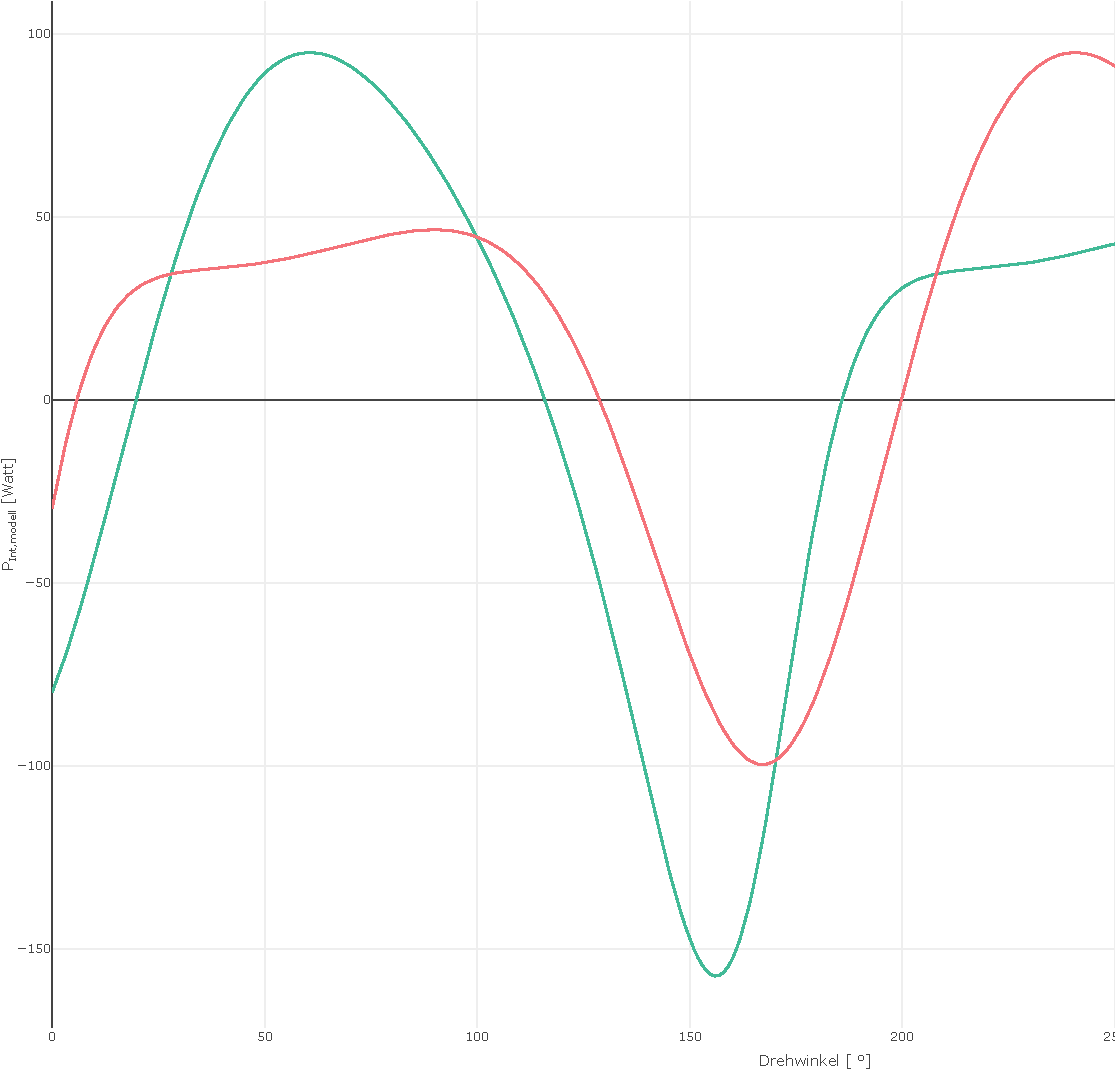
\includegraphics{Ergometer_Daten_files/figure-pdf/fig-PInt_Modell_Zyklus-1.pdf}

}

\caption{\label{fig-PInt_Modell_Zyklus}Beispielhafter Verlauf der
modellierten inneren Leistung (PInt,Modell) über einen kompletten
Pedalzyklus (360°), dargestellt mit positiven und negativen
Leistungsanteilen für das rechte (grün) und linke Bein (rot).}

\end{figure}%

Abbildung~\ref{fig-PInt_Modell_Zyklus_positiv} visualisiert im
Unterschied zu Abbildung~\ref{fig-PInt_Modell_Zyklus} ausschließlich die
positiven Leistungsanteile der P\textsubscript{Int,Modell}. Zusätzlich
ist der in diesem Beispiel berechnete Mittelwert der positiven
P\textsubscript{int,modell} Werte als horizontale Linie (grau
gestrichelt) eingezeichnet.

\begin{figure}

\centering{

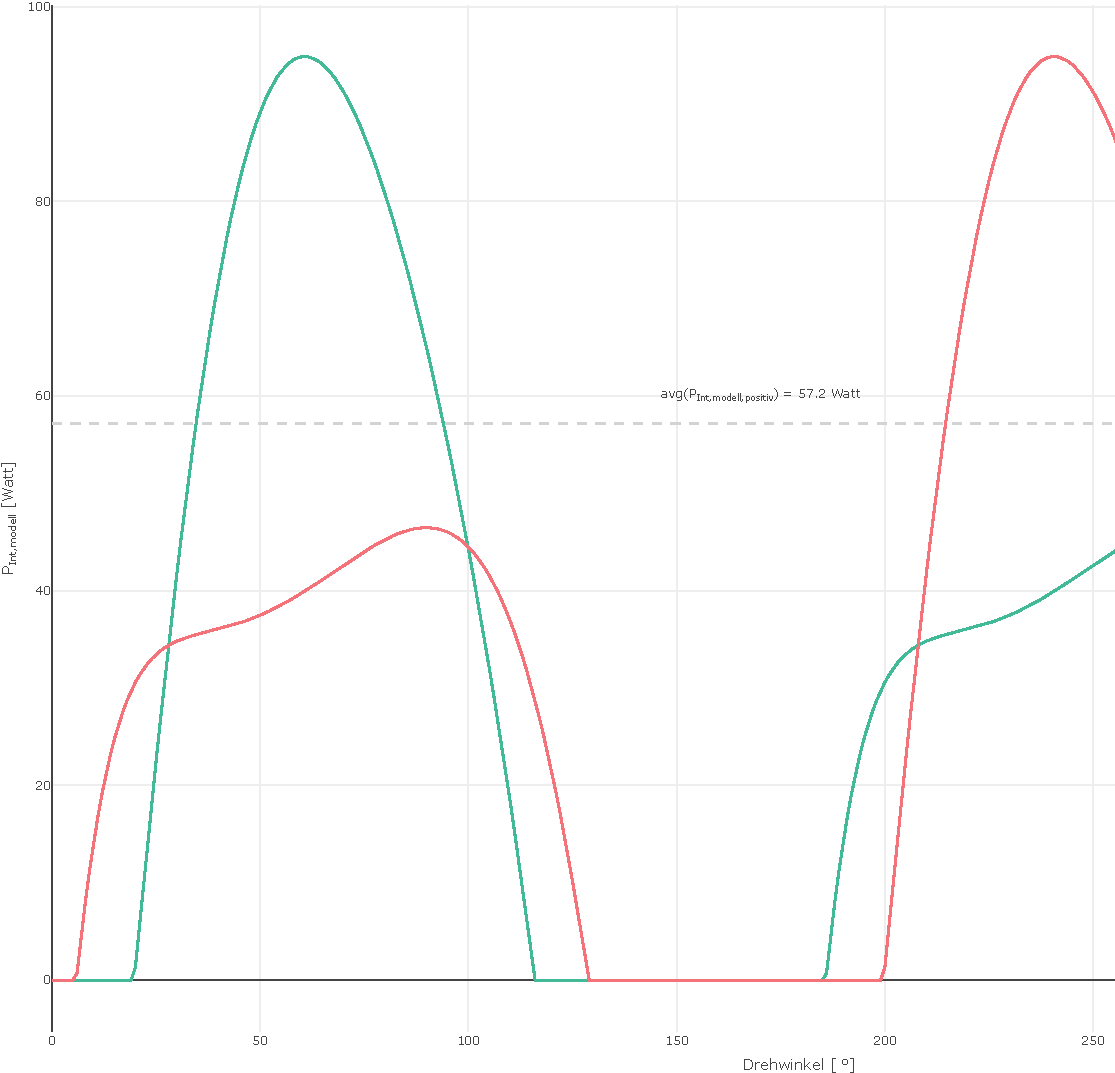
\includegraphics{Ergometer_Daten_files/figure-pdf/fig-PInt_Modell_Zyklus_positiv-1.pdf}

}

\caption{\label{fig-PInt_Modell_Zyklus_positiv}Beispielhafte Darstellung
der positiven Anteile der modellierten inneren Leistung beider Beine mit
berechneter P\textsubscript{int\_modell} als mittlerer Wert der
positiven P\textsubscript{int} Werte über einen vollständigen
Kurbelzyklus.}

\end{figure}%

\subsection{Zeitlicher Verlauf der aus der 3D-Kinematik modellierten
inneren Leistung während der
Pedalbewegung}\label{zeitlicher-verlauf-der-aus-der-3d-kinematik-modellierten-inneren-leistung-wuxe4hrend-der-pedalbewegung}

Die folgenden Abbildungen zeigen den zeitlichen Verlauf der aus der
3D-Kinematik berechneten positiven Anteile der inneren Leistung
(P\textsubscript{Int,Kinematik}) für den jeweiligen Messzeitraum.
Dargestellt sind die Leistungsverläufe des rechten (grün) und linken
(rot) Beins sowie der gemittelte P\textsubscript{Int,Kinematik}-Wert
(grau gestrichelt). Die interaktive Darstellung ermöglicht die Auswahl
verschiedener Probanden und deren jeweiliger Testdurchgänge.

\subsubsection{Proband 1}

\paragraph{Test 1}

\begin{figure}

\centering{

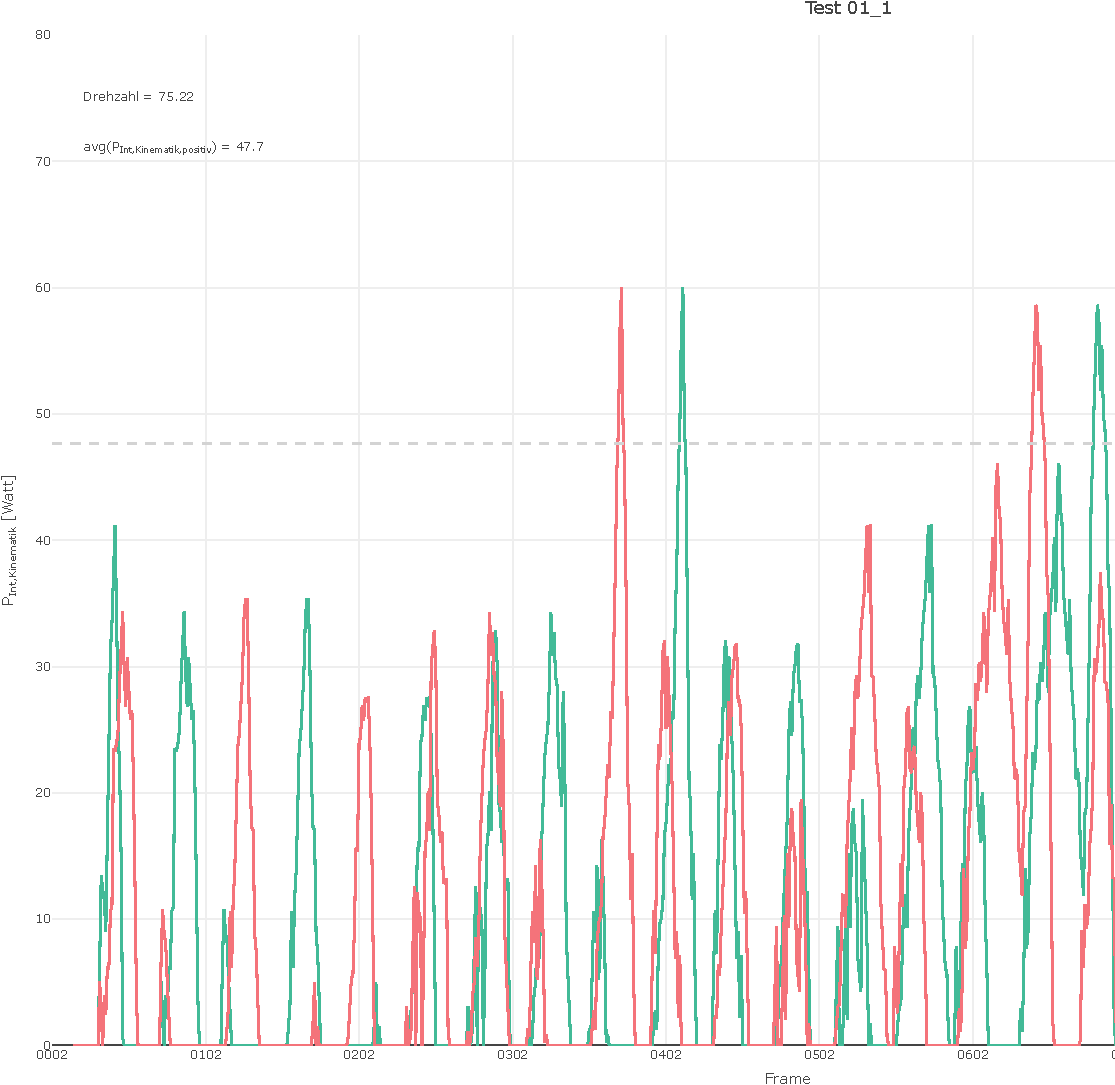
\includegraphics{Ergometer_Daten_files/figure-pdf/fig-PInt_Kinematik_01_1-1.pdf}

}

\caption{\label{fig-PInt_Kinematik_01_1}Zeitlicher Verlauf der aus der
3D-Kinematik berechneten positiven Anteile der inneren Leistung
(P\textsubscript{int}) beider Beine mit gemitteltem
P\textsubscript{int}-Wert (grau gestrichelt) für 01\_1.}

\end{figure}%

\paragraph{Test 2}

\begin{figure}

\centering{

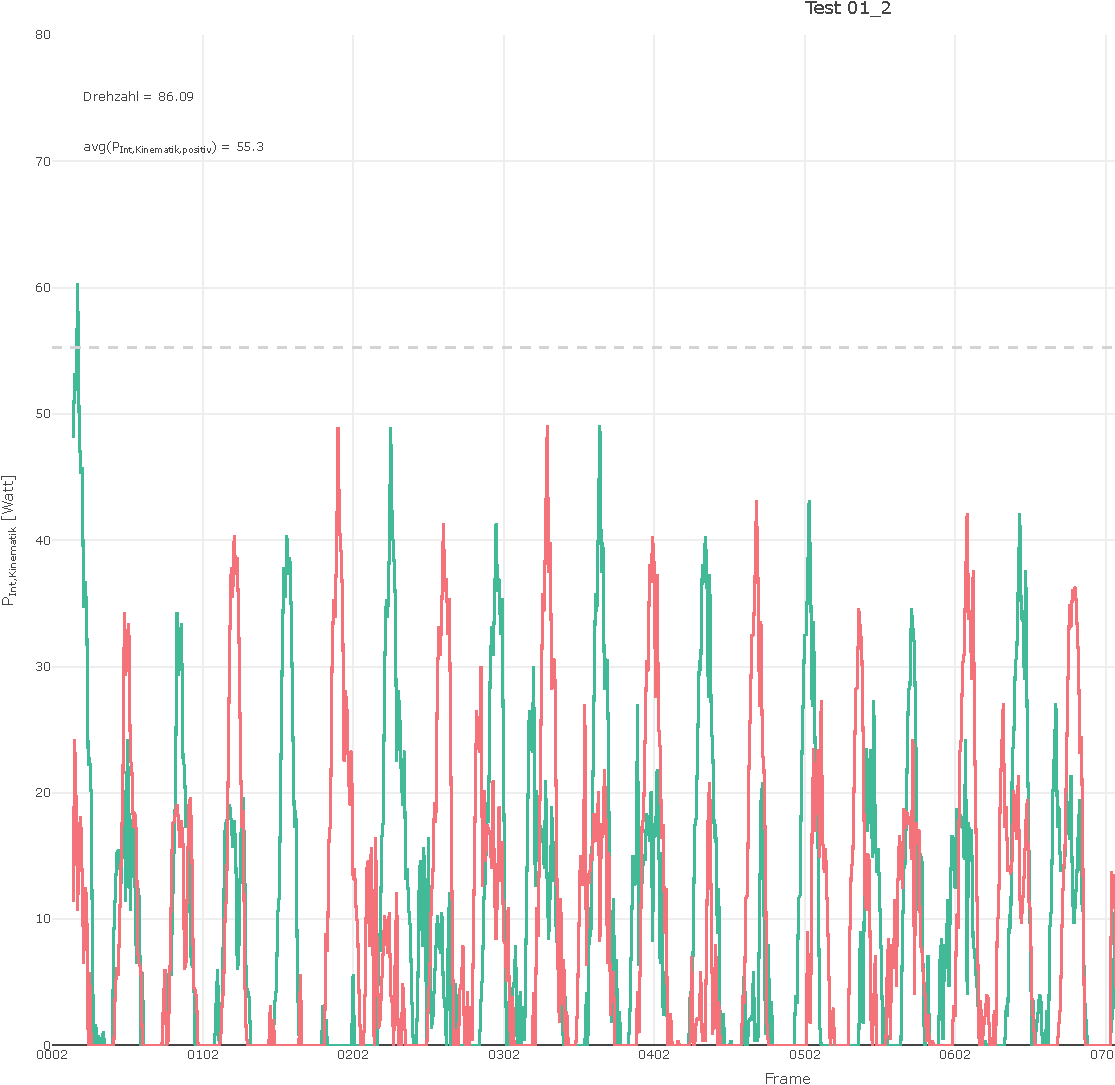
\includegraphics{Ergometer_Daten_files/figure-pdf/fig-PInt_Kinematik_01_2-1.pdf}

}

\caption{\label{fig-PInt_Kinematik_01_2}Zeitlicher Verlauf der aus der
3D-Kinematik berechneten positiven Anteile der inneren Leistung
(P\textsubscript{int}) beider Beine mit gemitteltem
P\textsubscript{int}-Wert (grau gestrichelt) für 01\_2.}

\end{figure}%

\paragraph{Test 3}

\begin{figure}

\centering{

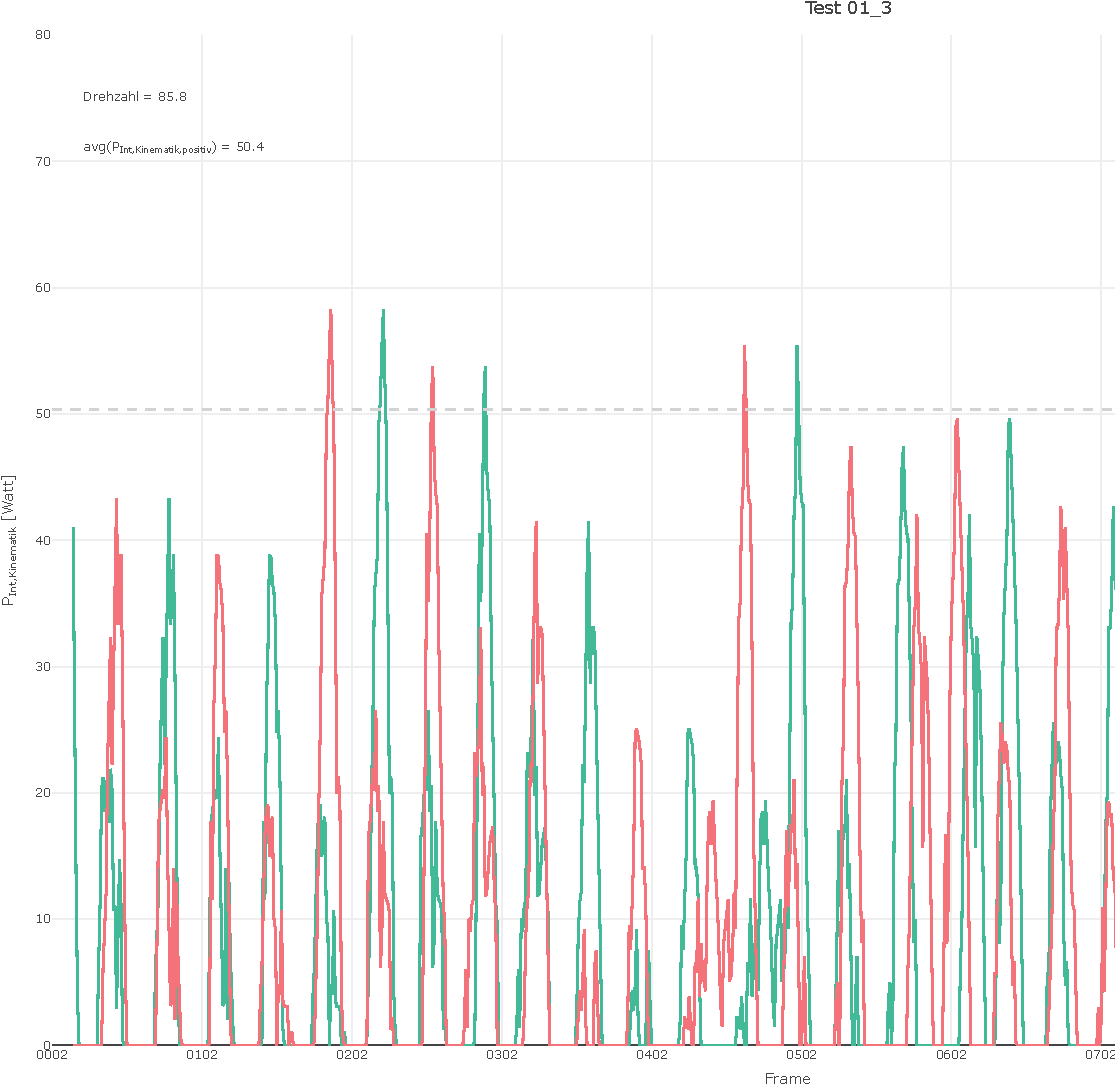
\includegraphics{Ergometer_Daten_files/figure-pdf/fig-PInt_Kinematik_01_3-1.pdf}

}

\caption{\label{fig-PInt_Kinematik_01_3}Zeitlicher Verlauf der aus der
3D-Kinematik berechneten positiven Anteile der inneren Leistung
(P\textsubscript{int}) beider Beine mit gemitteltem
P\textsubscript{int}-Wert (grau gestrichelt) für 01\_3.}

\end{figure}%

\paragraph{Test 4}

\begin{figure}

\centering{

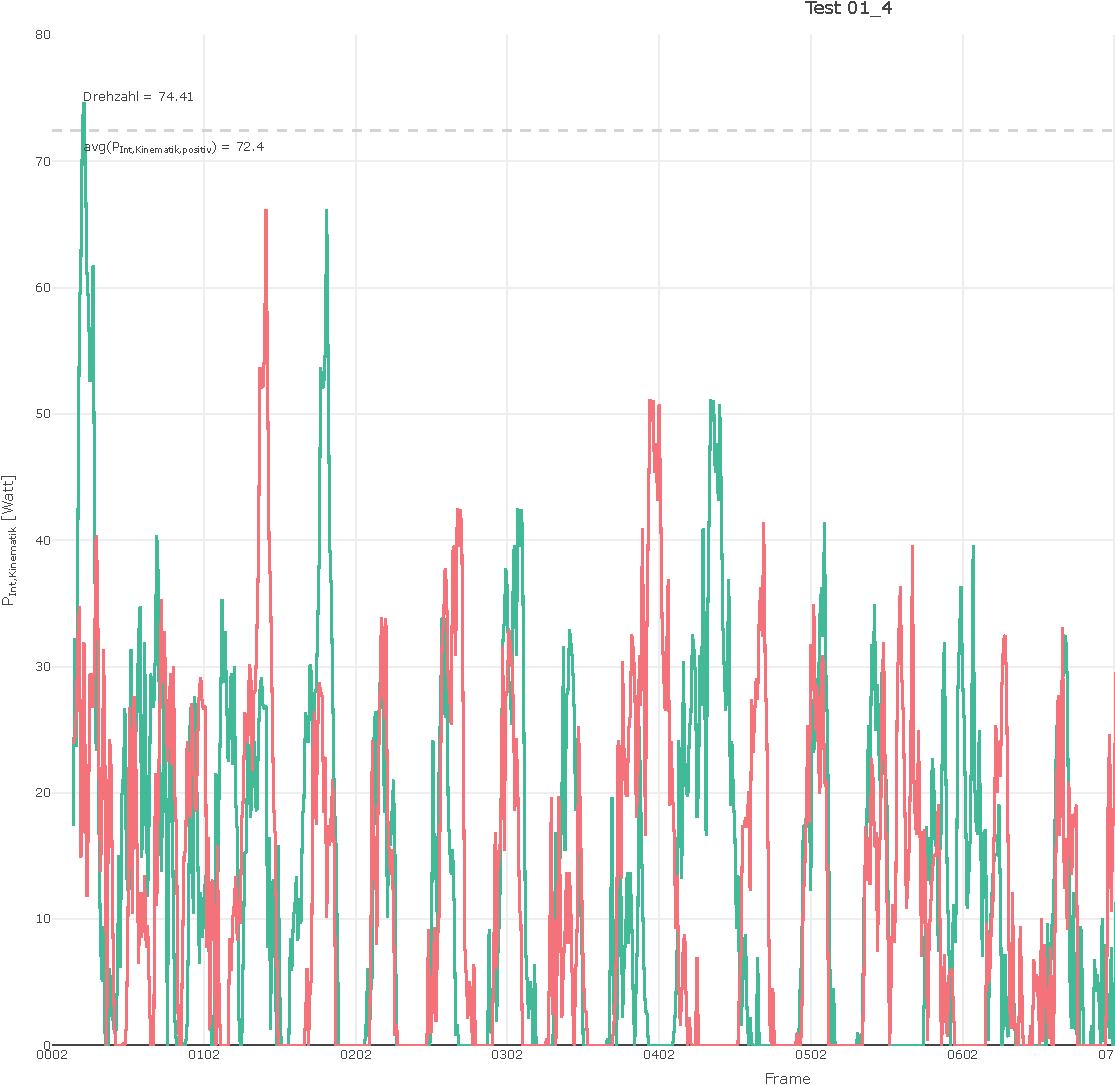
\includegraphics{Ergometer_Daten_files/figure-pdf/fig-PInt_Kinematik_01_4-1.pdf}

}

\caption{\label{fig-PInt_Kinematik_01_4}Zeitlicher Verlauf der aus der
3D-Kinematik berechneten positiven Anteile der inneren Leistung
(P\textsubscript{int}) beider Beine mit gemitteltem
P\textsubscript{int}-Wert (grau gestrichelt) für 01\_4.}

\end{figure}%

\paragraph{Test 5}

\begin{figure}

\centering{

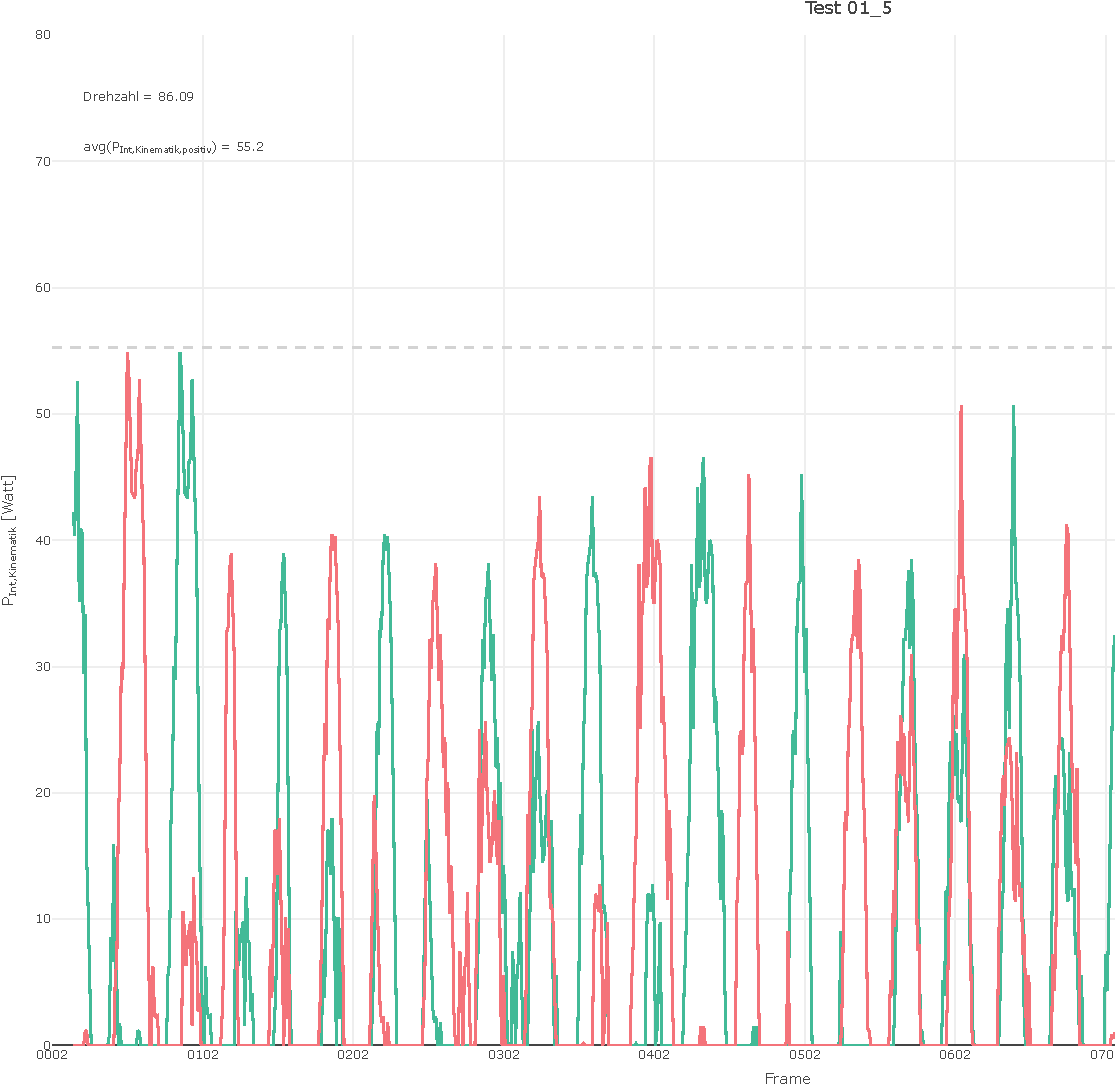
\includegraphics{Ergometer_Daten_files/figure-pdf/fig-PInt_Kinematik_01_5-1.pdf}

}

\caption{\label{fig-PInt_Kinematik_01_5}Zeitlicher Verlauf der aus der
3D-Kinematik berechneten positiven Anteile der inneren Leistung
(P\textsubscript{int}) beider Beine mit gemitteltem
P\textsubscript{int}-Wert (grau gestrichelt) für 01\_5.}

\end{figure}%

\paragraph{Test 6}

\begin{figure}

\centering{

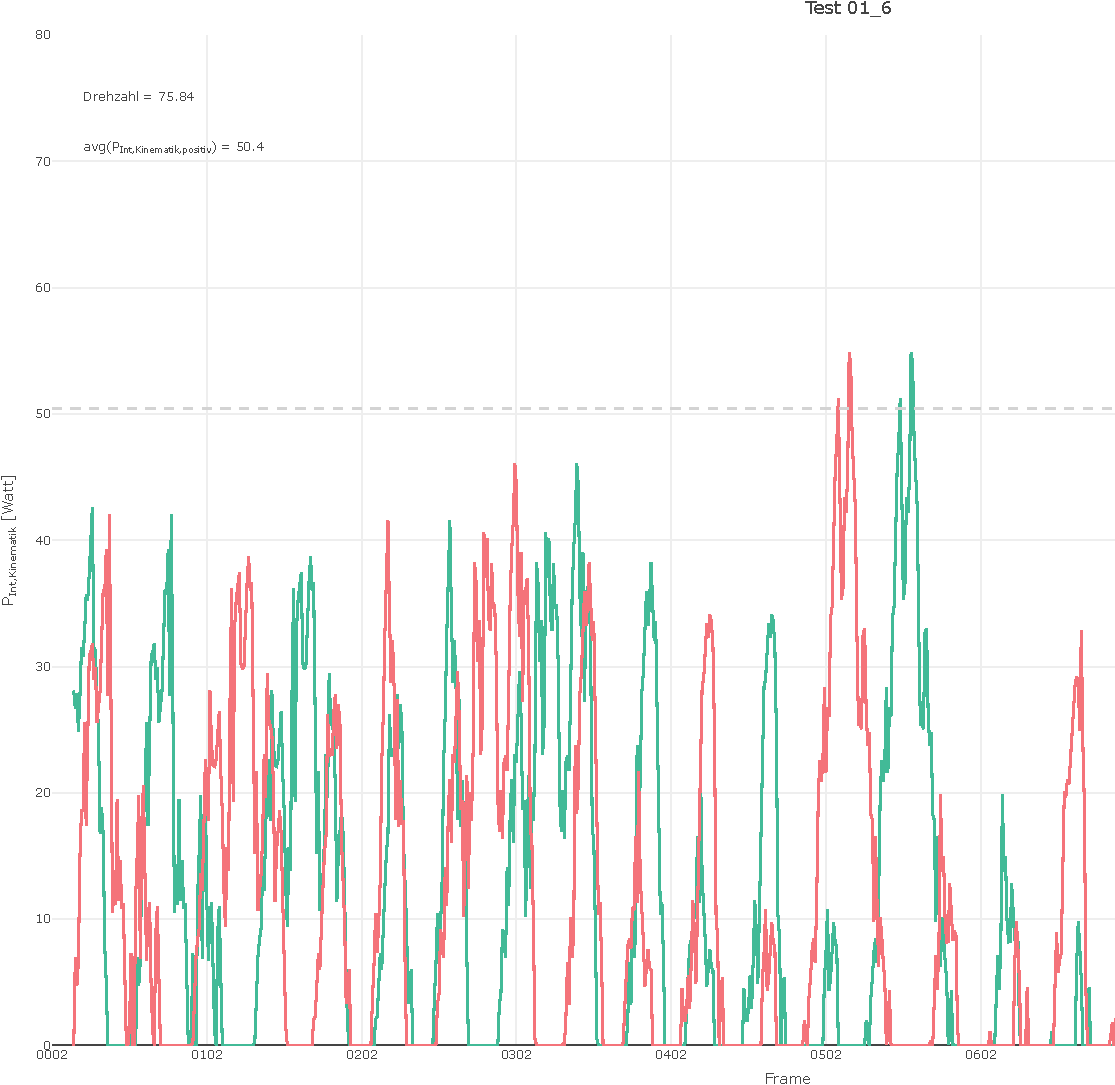
\includegraphics{Ergometer_Daten_files/figure-pdf/fig-PInt_Kinematik_01_6-1.pdf}

}

\caption{\label{fig-PInt_Kinematik_01_6}Zeitlicher Verlauf der aus der
3D-Kinematik berechneten positiven Anteile der inneren Leistung
(P\textsubscript{int}) beider Beine mit gemitteltem
P\textsubscript{int}-Wert (grau gestrichelt) für 01\_6.}

\end{figure}%

\subsubsection{Proband 6}

\paragraph{Test 2}

\begin{figure}

\centering{

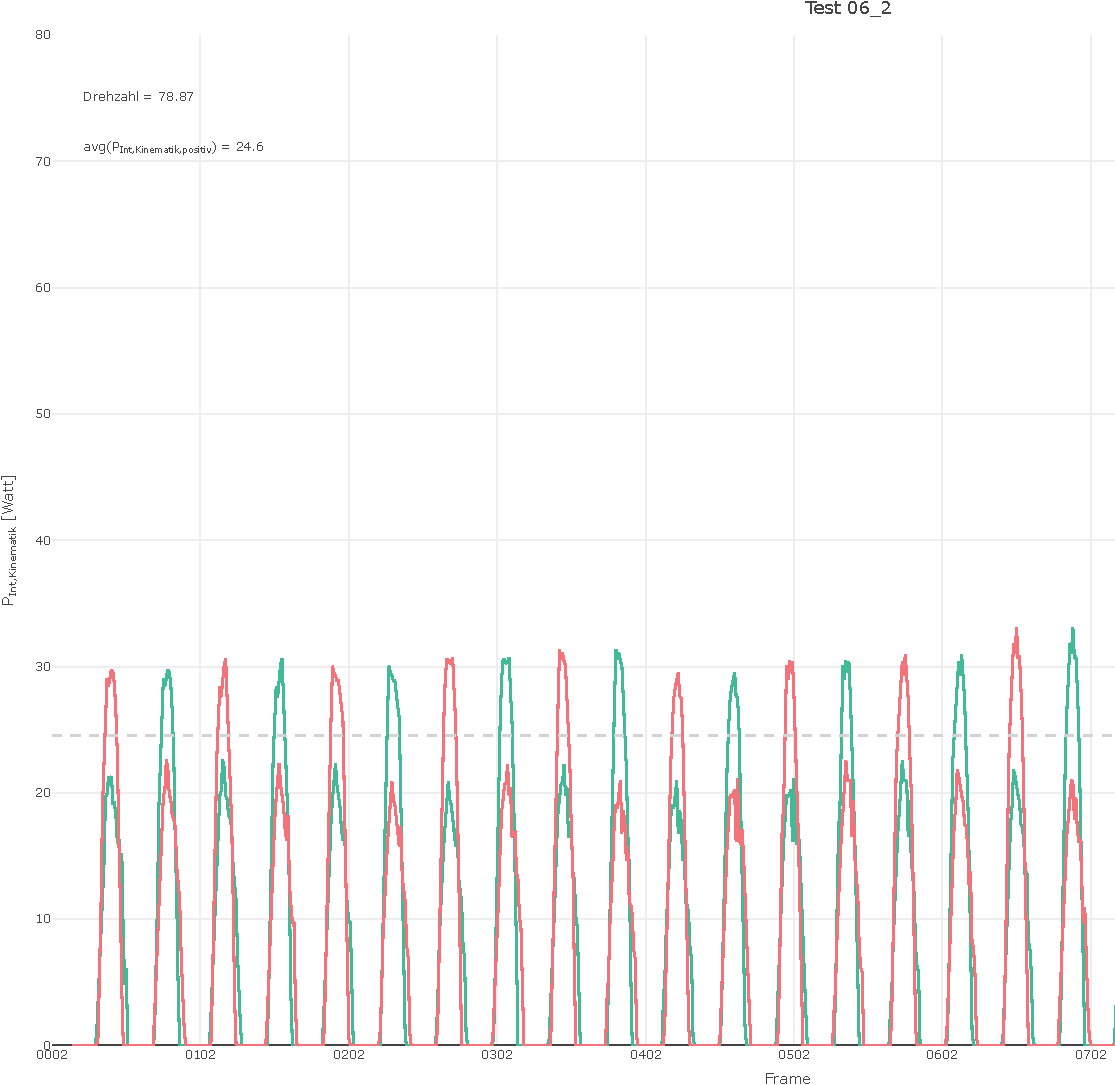
\includegraphics{Ergometer_Daten_files/figure-pdf/fig-PInt_Kinematik_06_2-1.pdf}

}

\caption{\label{fig-PInt_Kinematik_06_2}Zeitlicher Verlauf der aus der
3D-Kinematik berechneten positiven Anteile der inneren Leistung
(P\textsubscript{int}) beider Beine mit gemitteltem
P\textsubscript{int}-Wert (grau gestrichelt) für 06\_2.}

\end{figure}%

\paragraph{Test 3}

\begin{figure}

\centering{

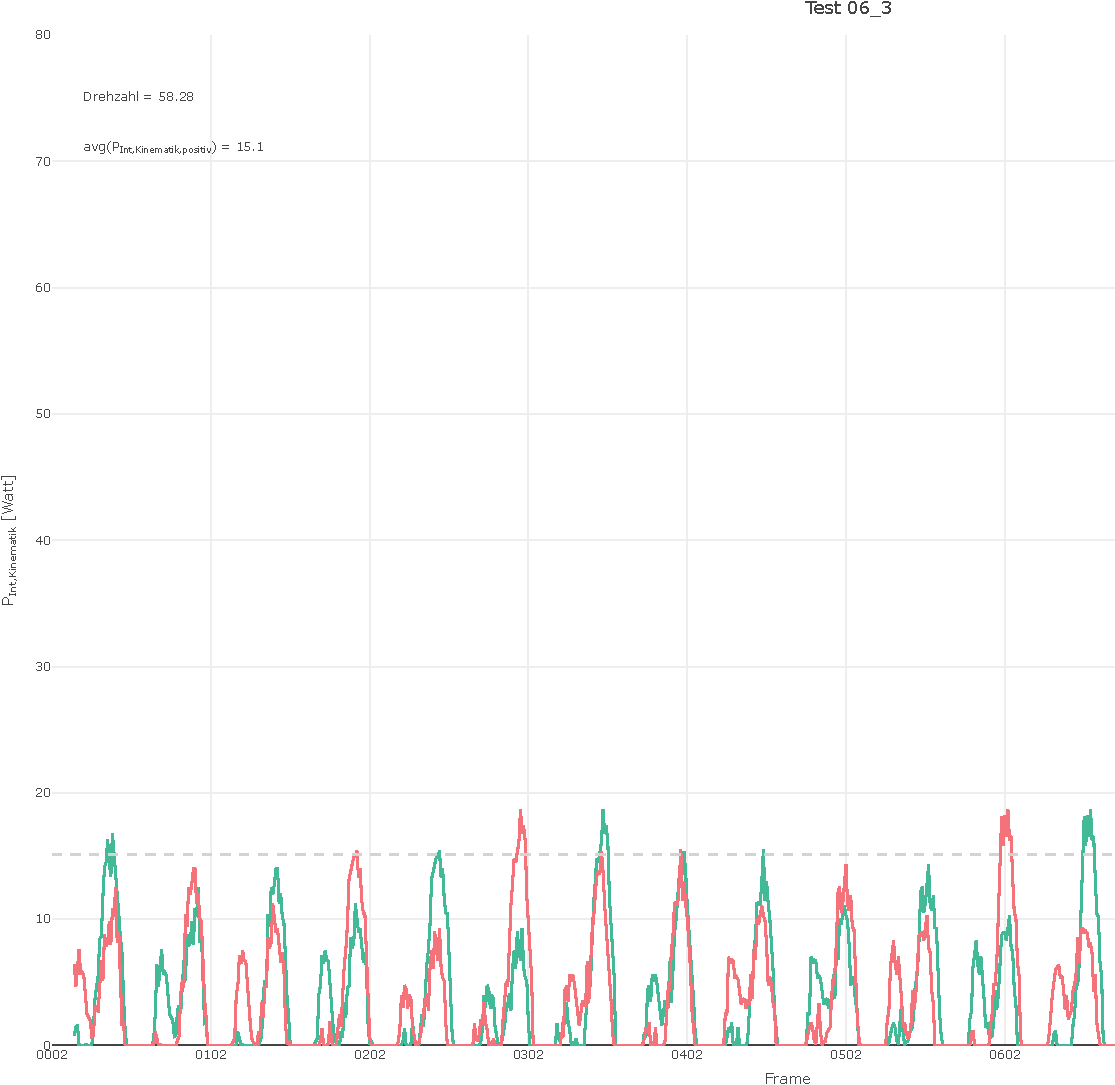
\includegraphics{Ergometer_Daten_files/figure-pdf/fig-PInt_Kinematik_06_3-1.pdf}

}

\caption{\label{fig-PInt_Kinematik_06_3}Zeitlicher Verlauf der aus der
3D-Kinematik berechneten positiven Anteile der inneren Leistung
(P\textsubscript{int}) beider Beine mit gemitteltem
P\textsubscript{int}-Wert (grau gestrichelt) für 06\_3.}

\end{figure}%

\paragraph{Test 4}

\begin{figure}

\centering{

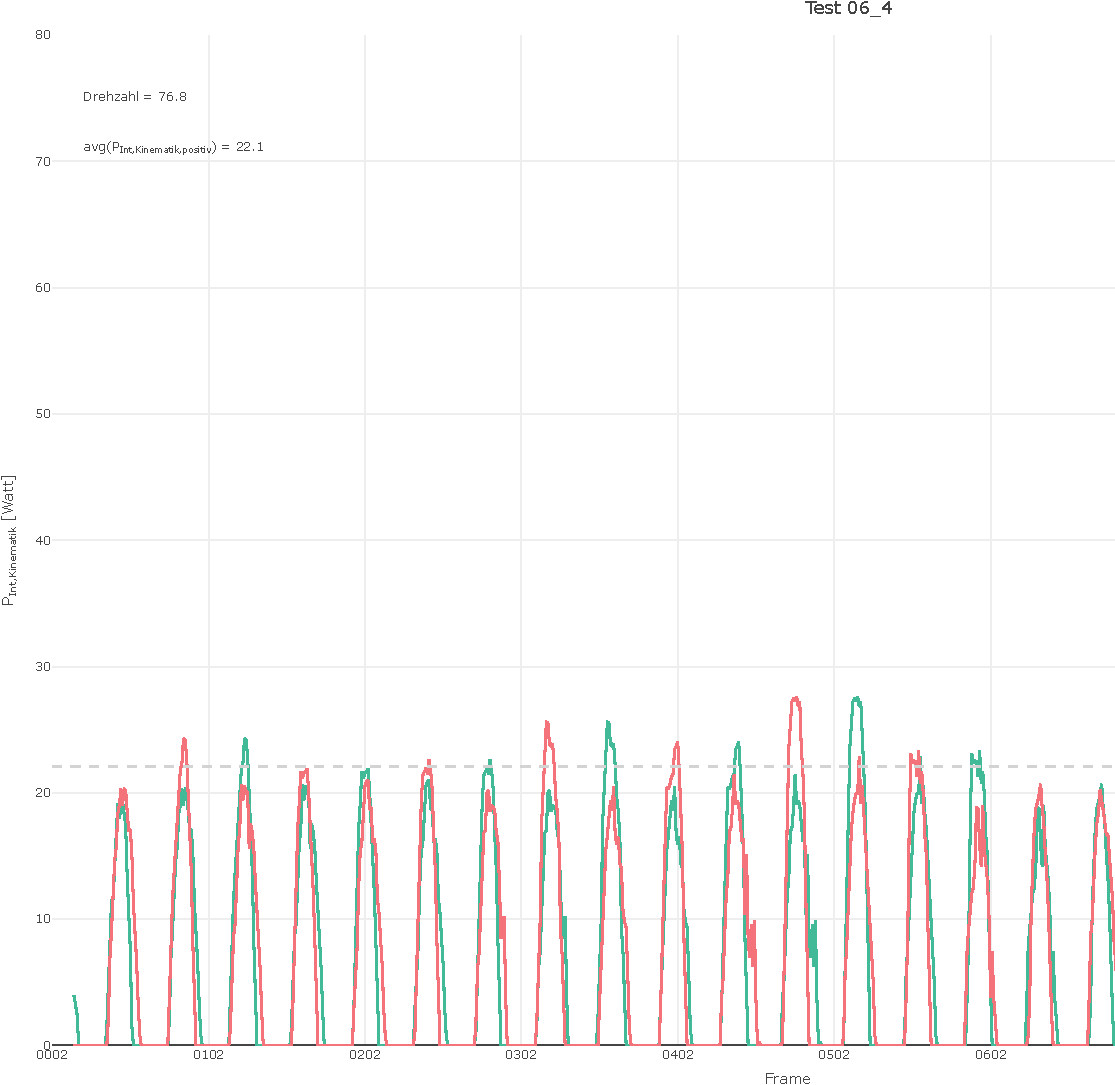
\includegraphics{Ergometer_Daten_files/figure-pdf/fig-PInt_Kinematik_06_4-1.pdf}

}

\caption{\label{fig-PInt_Kinematik_06_4}Zeitlicher Verlauf der aus der
3D-Kinematik berechneten positiven Anteile der inneren Leistung
(P\textsubscript{int}) beider Beine mit gemitteltem
P\textsubscript{int}-Wert (grau gestrichelt) für 06\_4.}

\end{figure}%

\paragraph{Test 5}

\begin{figure}

\centering{

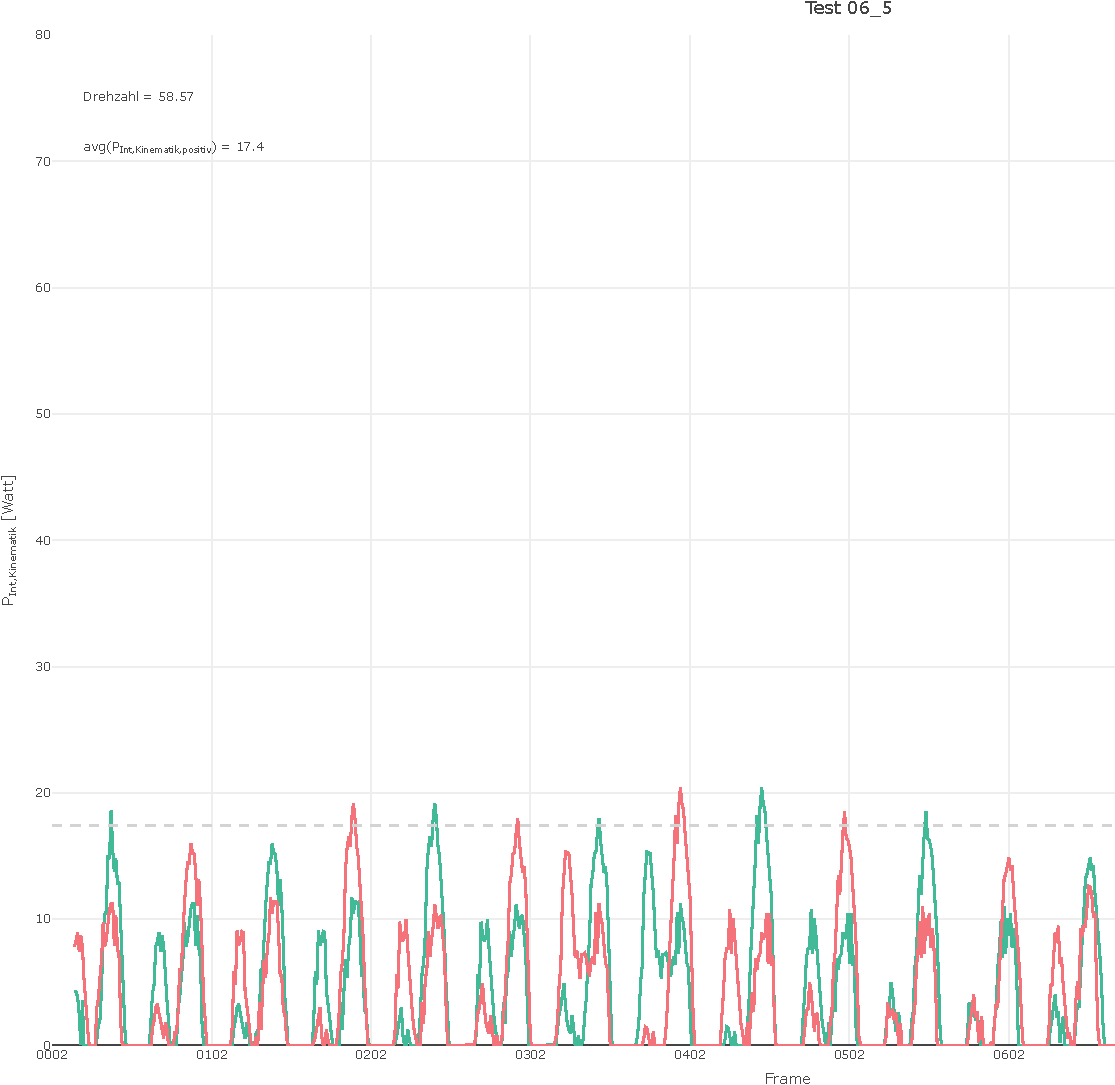
\includegraphics{Ergometer_Daten_files/figure-pdf/fig-PInt_Kinematik_06_5-1.pdf}

}

\caption{\label{fig-PInt_Kinematik_06_5}Zeitlicher Verlauf der aus der
3D-Kinematik berechneten positiven Anteile der inneren Leistung
(P\textsubscript{int}) beider Beine mit gemitteltem
P\textsubscript{int}-Wert (grau gestrichelt) für 06\_5.}

\end{figure}%

\paragraph{Test 6}

\begin{figure}

\centering{

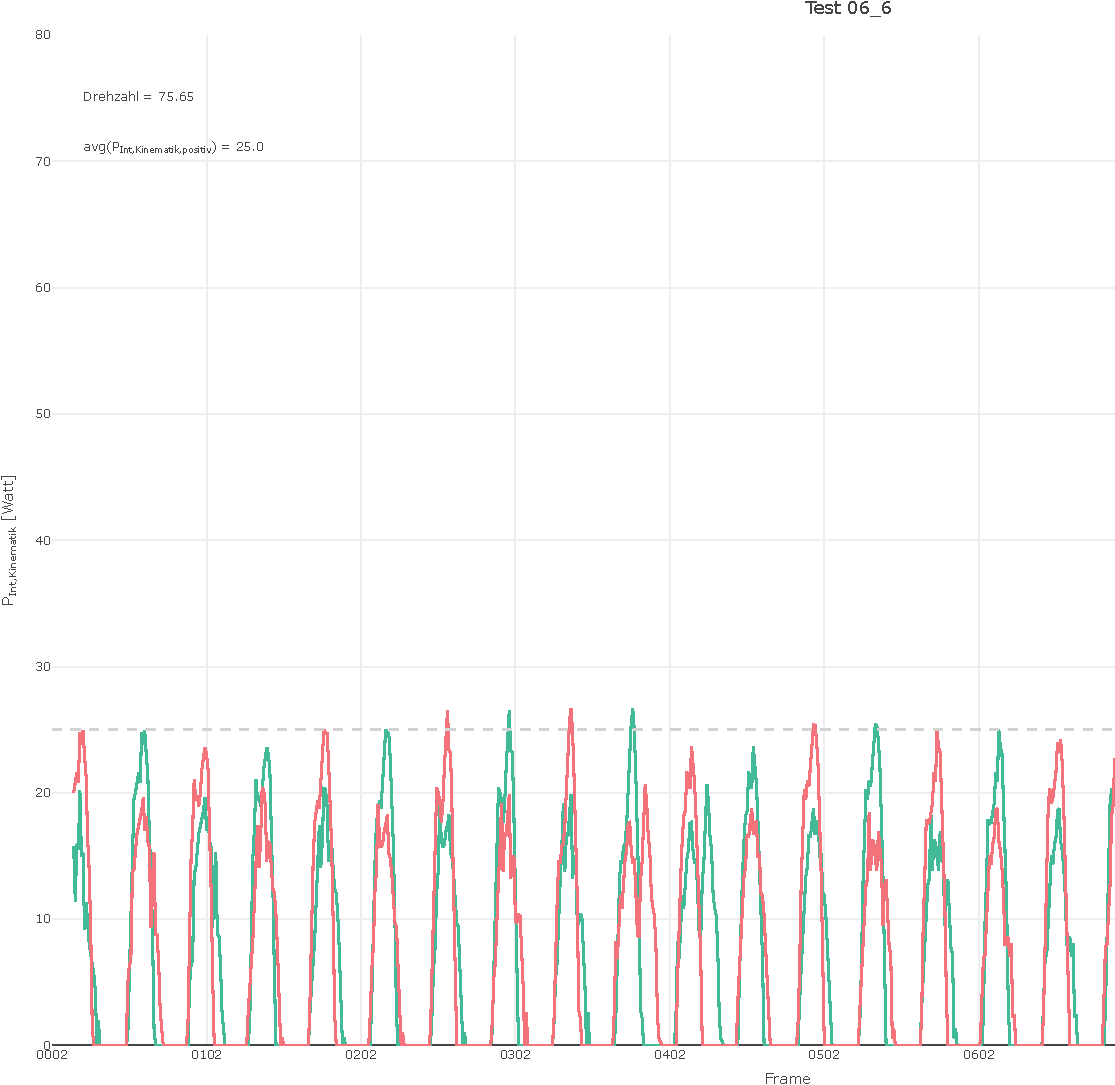
\includegraphics{Ergometer_Daten_files/figure-pdf/fig-PInt_Kinematik_06_6-1.pdf}

}

\caption{\label{fig-PInt_Kinematik_06_6}Zeitlicher Verlauf der aus der
3D-Kinematik berechneten positiven Anteile der inneren Leistung
(P\textsubscript{int}) beider Beine mit gemitteltem
P\textsubscript{int}-Wert (grau gestrichelt) für 06\_6.}

\end{figure}%

\subsubsection{Proband 13}

\paragraph{Test 3}

\begin{figure}

\centering{

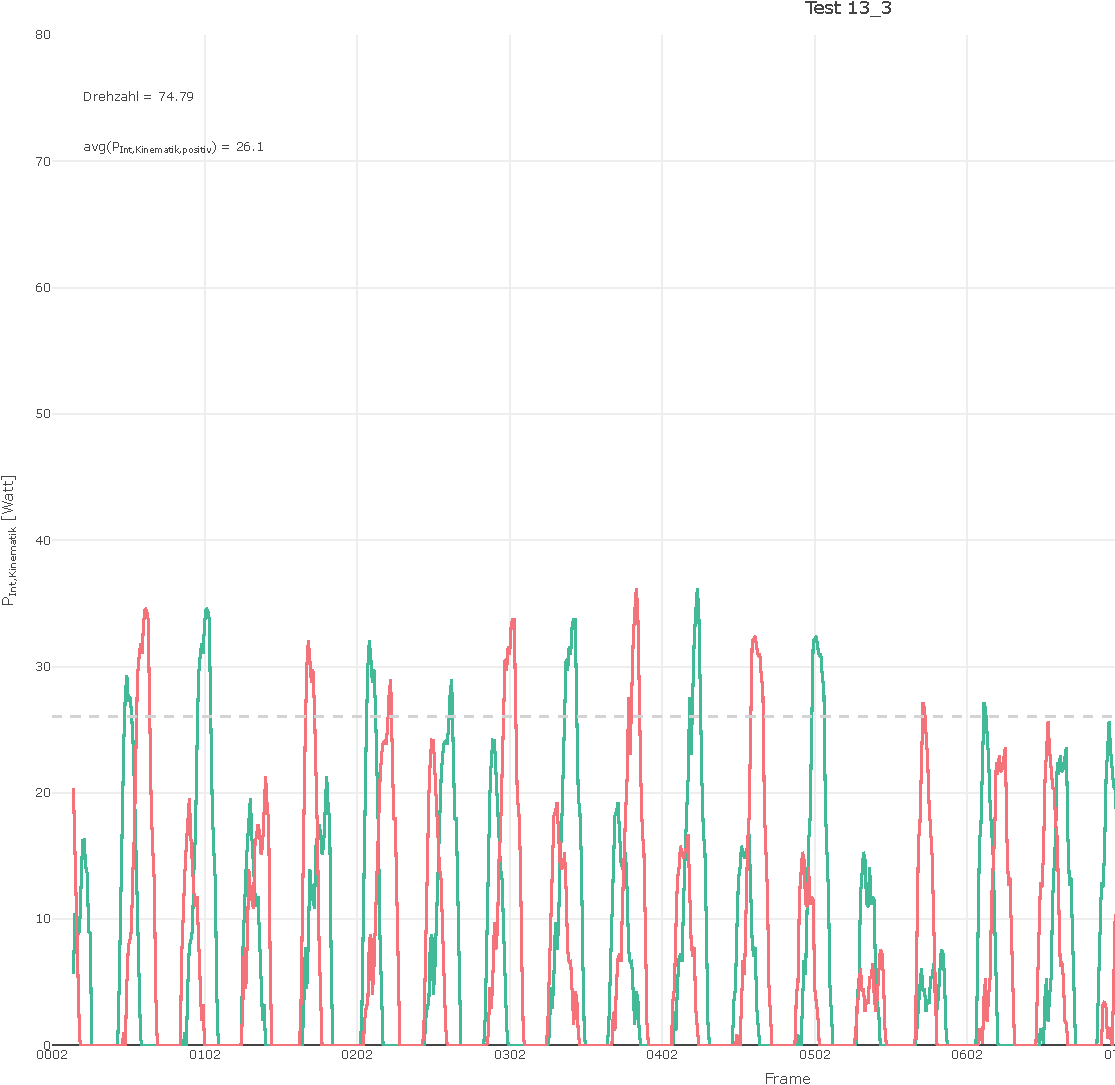
\includegraphics{Ergometer_Daten_files/figure-pdf/fig-PInt_Kinematik_13_3-1.pdf}

}

\caption{\label{fig-PInt_Kinematik_13_3}Zeitlicher Verlauf der aus der
3D-Kinematik berechneten positiven Anteile der inneren Leistung
(P\textsubscript{int}) beider Beine mit gemitteltem
P\textsubscript{int}-Wert (grau gestrichelt) für 13\_3.}

\end{figure}%

\paragraph{Test 4}

\begin{figure}

\centering{

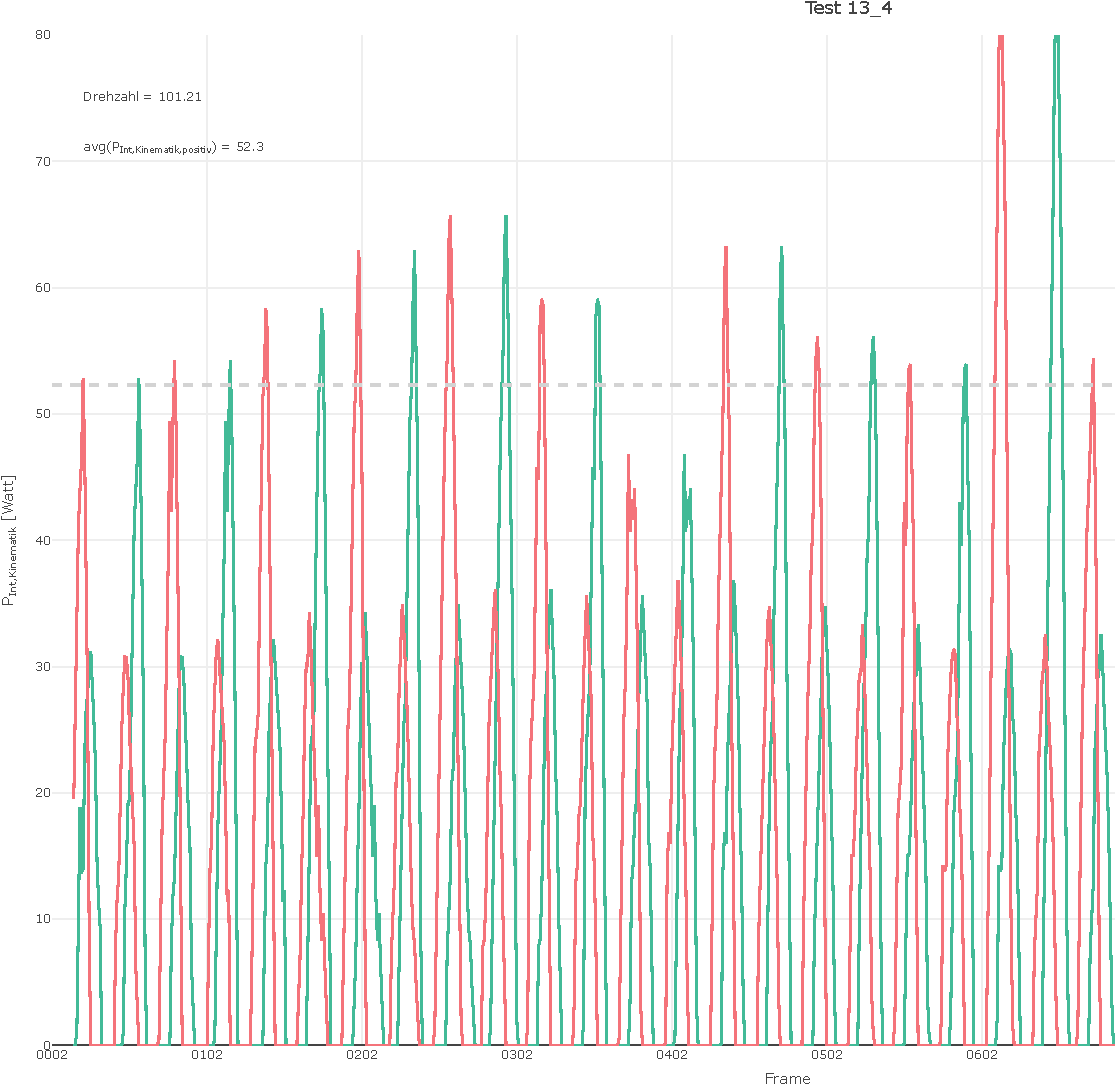
\includegraphics{Ergometer_Daten_files/figure-pdf/fig-PInt_Kinematik_13_4-1.pdf}

}

\caption{\label{fig-PInt_Kinematik_13_4}Zeitlicher Verlauf der aus der
3D-Kinematik berechneten positiven Anteile der inneren Leistung
(P\textsubscript{int}) beider Beine mit gemitteltem
P\textsubscript{int}-Wert (grau gestrichelt) für 13\_4.}

\end{figure}%

\paragraph{Test 5}

\begin{figure}

\centering{

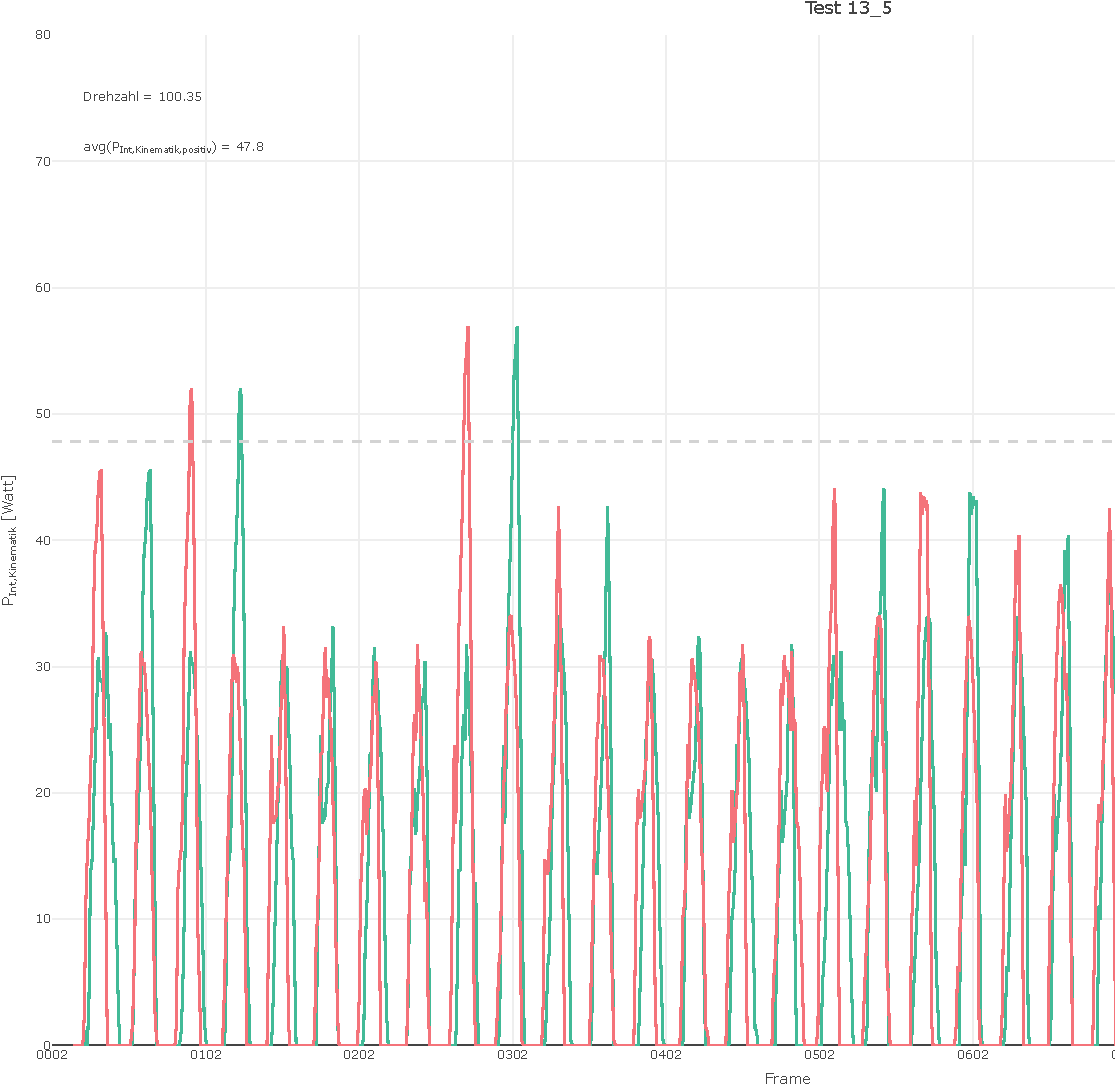
\includegraphics{Ergometer_Daten_files/figure-pdf/fig-PInt_Kinematik_13_5-1.pdf}

}

\caption{\label{fig-PInt_Kinematik_13_5}Zeitlicher Verlauf der aus der
3D-Kinematik berechneten positiven Anteile der inneren Leistung
(P\textsubscript{int}) beider Beine mit gemitteltem
P\textsubscript{int}-Wert (grau gestrichelt) für 13\_5.}

\end{figure}%

\paragraph{Test 6}

\begin{figure}

\centering{

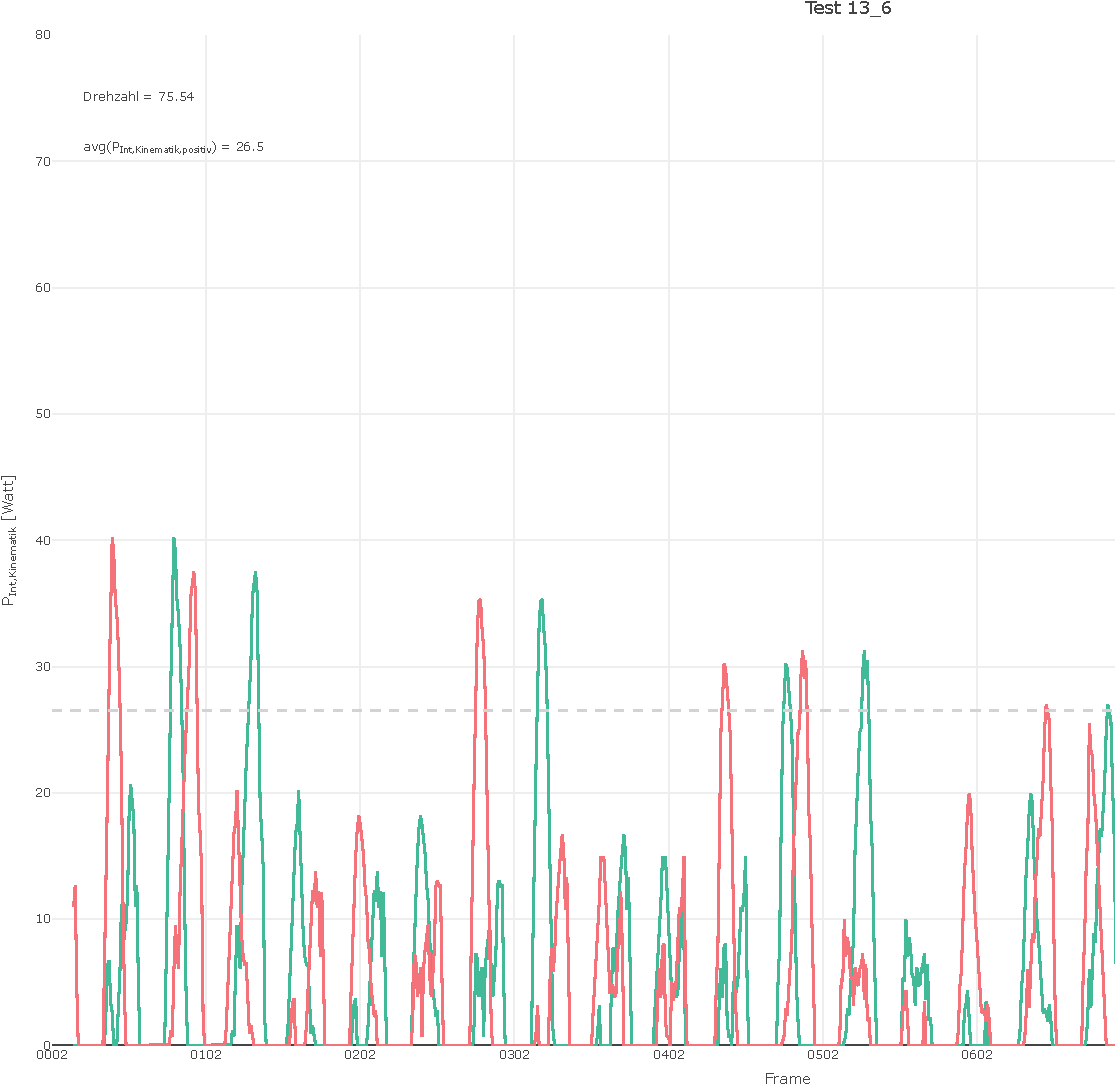
\includegraphics{Ergometer_Daten_files/figure-pdf/fig-PInt_Kinematik_13_6-1.pdf}

}

\caption{\label{fig-PInt_Kinematik_13_6}Zeitlicher Verlauf der aus der
3D-Kinematik berechneten positiven Anteile der inneren Leistung
(P\textsubscript{int}) beider Beine mit gemitteltem
P\textsubscript{int}-Wert (grau gestrichelt) für 13\_6.}

\end{figure}%

\subsubsection{Proband 15}

\paragraph{Test 1}

\begin{figure}

\centering{

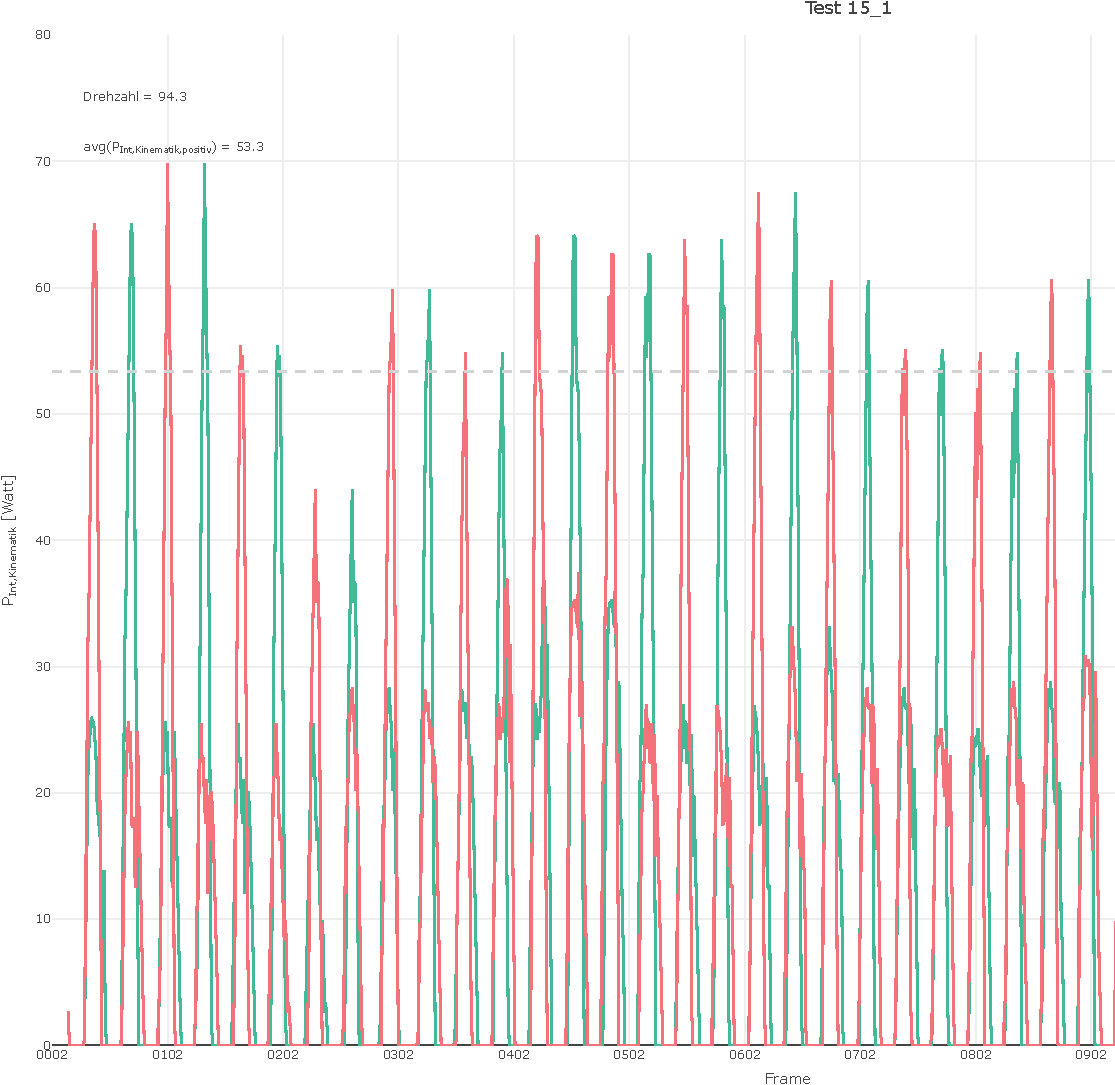
\includegraphics{Ergometer_Daten_files/figure-pdf/fig-PInt_Kinematik_15_1-1.pdf}

}

\caption{\label{fig-PInt_Kinematik_15_1}Zeitlicher Verlauf der aus der
3D-Kinematik berechneten positiven Anteile der inneren Leistung
(P\textsubscript{int}) beider Beine mit gemitteltem
P\textsubscript{int}-Wert (grau gestrichelt) für 15\_1.}

\end{figure}%

\paragraph{Test 2}

\begin{figure}

\centering{

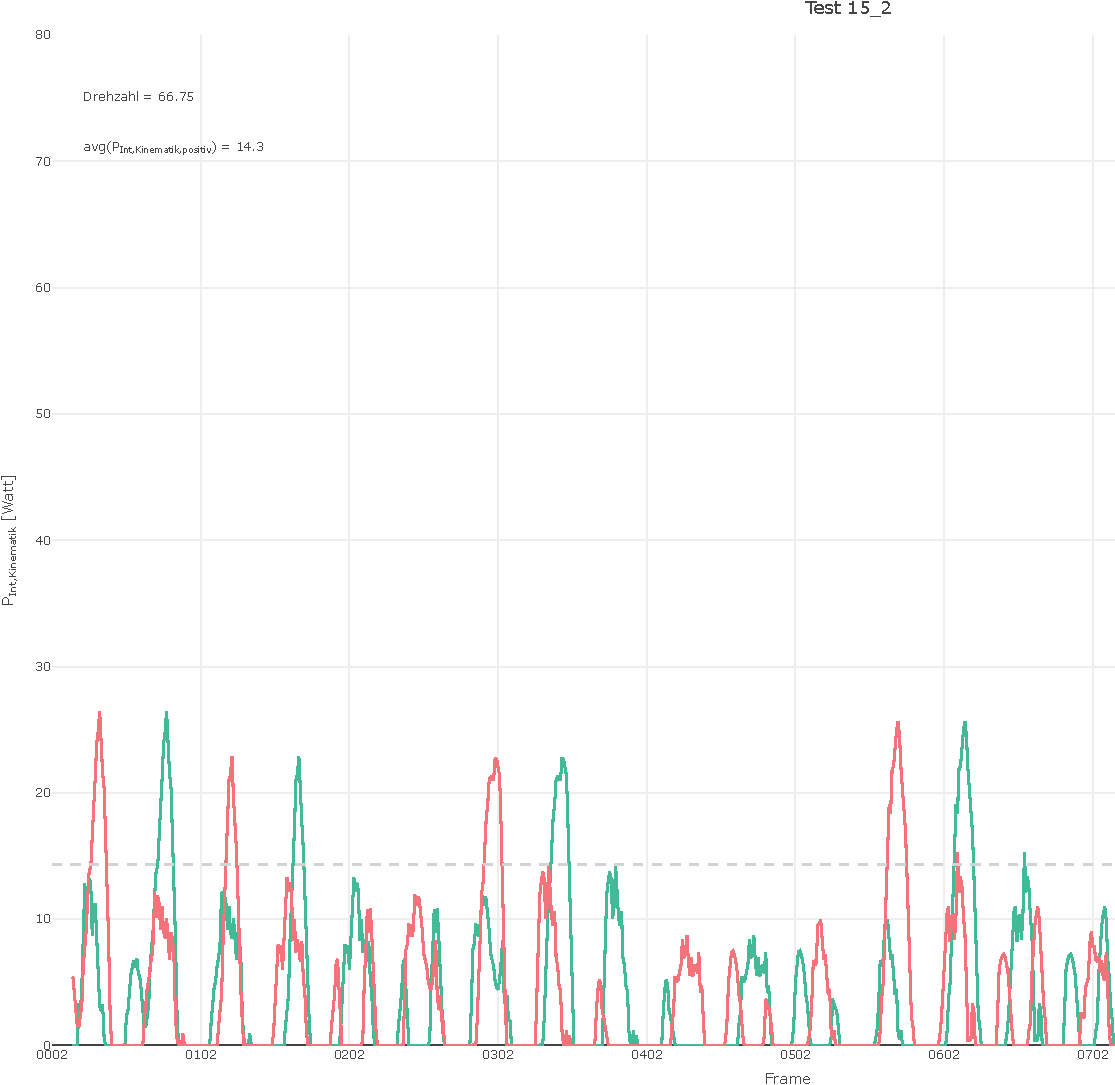
\includegraphics{Ergometer_Daten_files/figure-pdf/fig-PInt_Kinematik_15_2-1.pdf}

}

\caption{\label{fig-PInt_Kinematik_15_2}Zeitlicher Verlauf der aus der
3D-Kinematik berechneten positiven Anteile der inneren Leistung
(P\textsubscript{int}) beider Beine mit gemitteltem
P\textsubscript{int}-Wert (grau gestrichelt) für 15\_2.}

\end{figure}%

\paragraph{Test 3}

\begin{figure}

\centering{

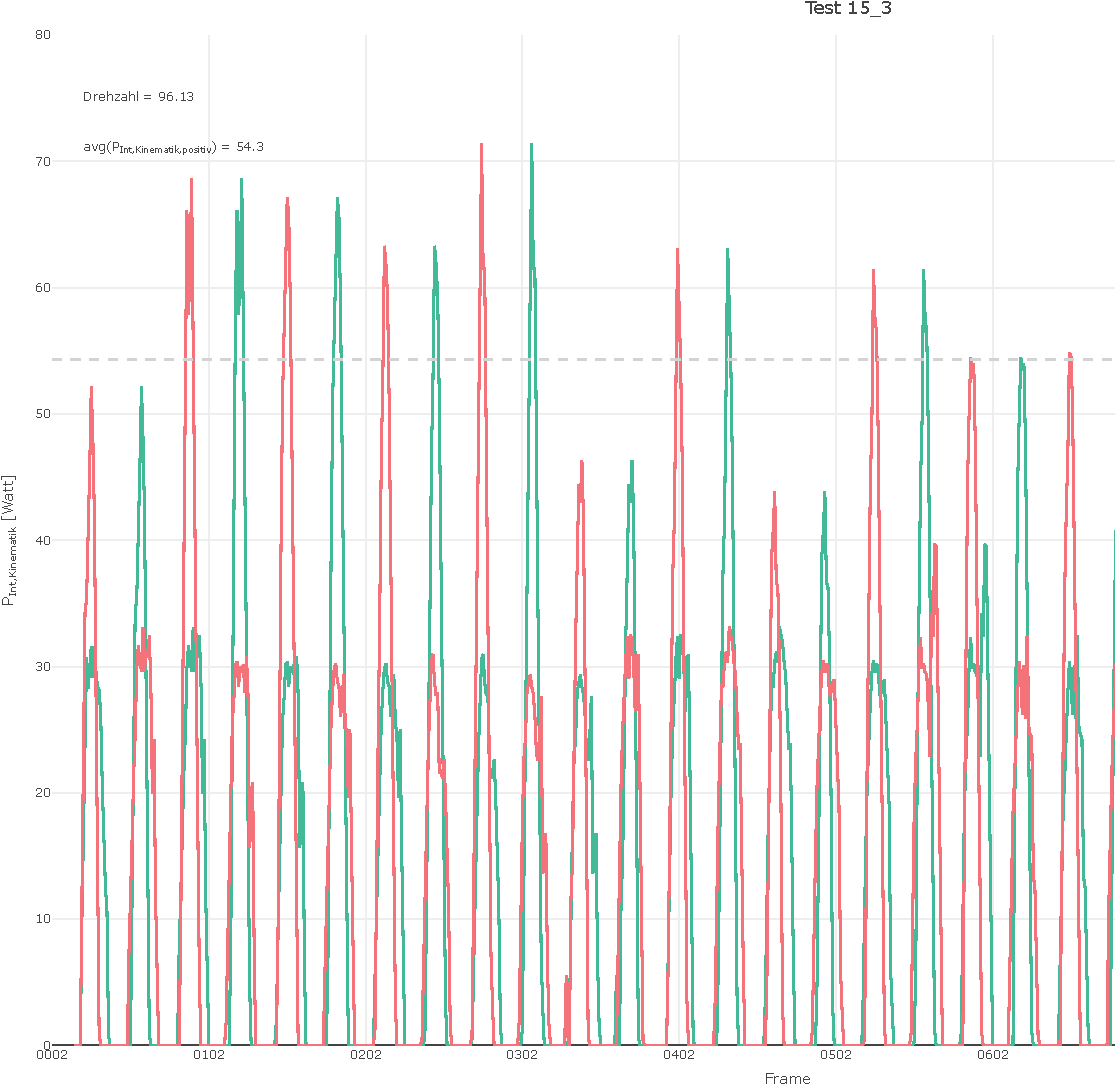
\includegraphics{Ergometer_Daten_files/figure-pdf/fig-PInt_Kinematik_15_3-1.pdf}

}

\caption{\label{fig-PInt_Kinematik_15_3}Zeitlicher Verlauf der aus der
3D-Kinematik berechneten positiven Anteile der inneren Leistung
(P\textsubscript{int}) beider Beine mit gemitteltem
P\textsubscript{int}-Wert (grau gestrichelt) für 15\_3.}

\end{figure}%

\paragraph{Test 4}

\begin{figure}

\centering{

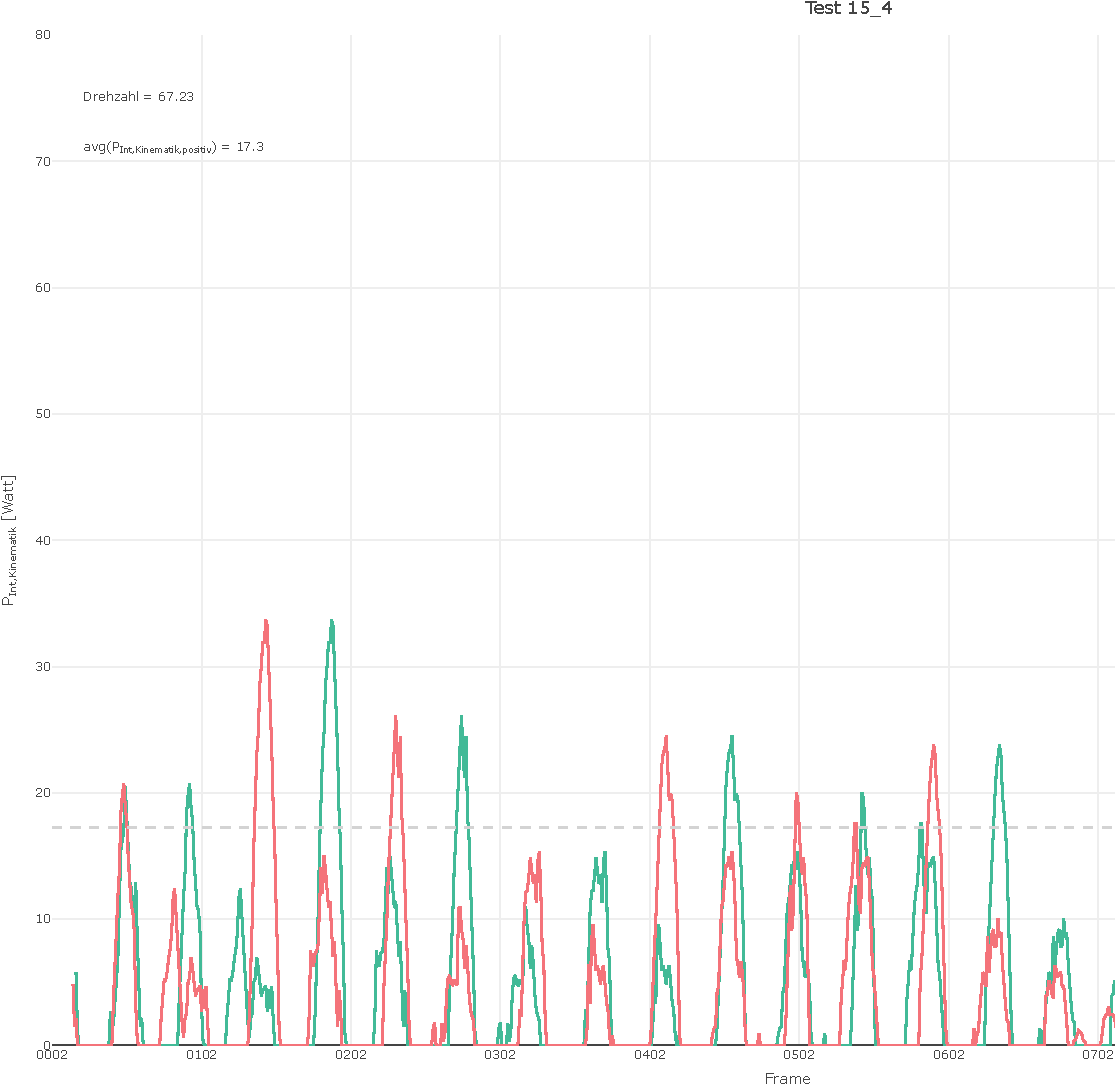
\includegraphics{Ergometer_Daten_files/figure-pdf/fig-PInt_Kinematik_15_4-1.pdf}

}

\caption{\label{fig-PInt_Kinematik_15_4}Zeitlicher Verlauf der aus der
3D-Kinematik berechneten positiven Anteile der inneren Leistung
(P\textsubscript{int}) beider Beine mit gemitteltem
P\textsubscript{int}-Wert (grau gestrichelt) für 15\_4.}

\end{figure}%

\paragraph{Test 5}

\begin{figure}

\centering{

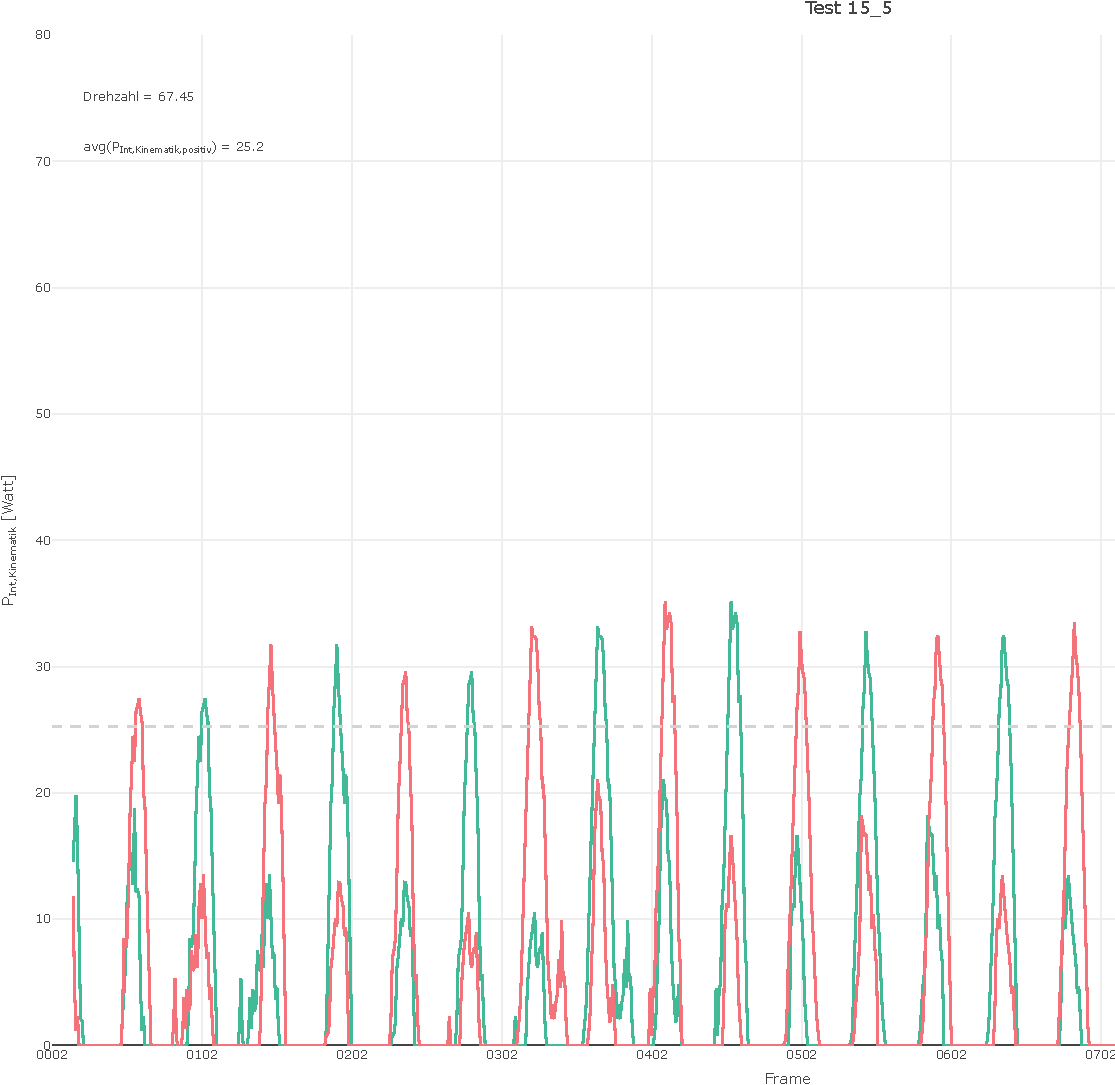
\includegraphics{Ergometer_Daten_files/figure-pdf/fig-PInt_Kinematik_15_5-1.pdf}

}

\caption{\label{fig-PInt_Kinematik_15_5}Zeitlicher Verlauf der aus der
3D-Kinematik berechneten positiven Anteile der inneren Leistung
(P\textsubscript{int}) beider Beine mit gemitteltem
P\textsubscript{int}-Wert (grau gestrichelt) für 15\_5.}

\end{figure}%

\paragraph{Test 6}

\begin{figure}

\centering{

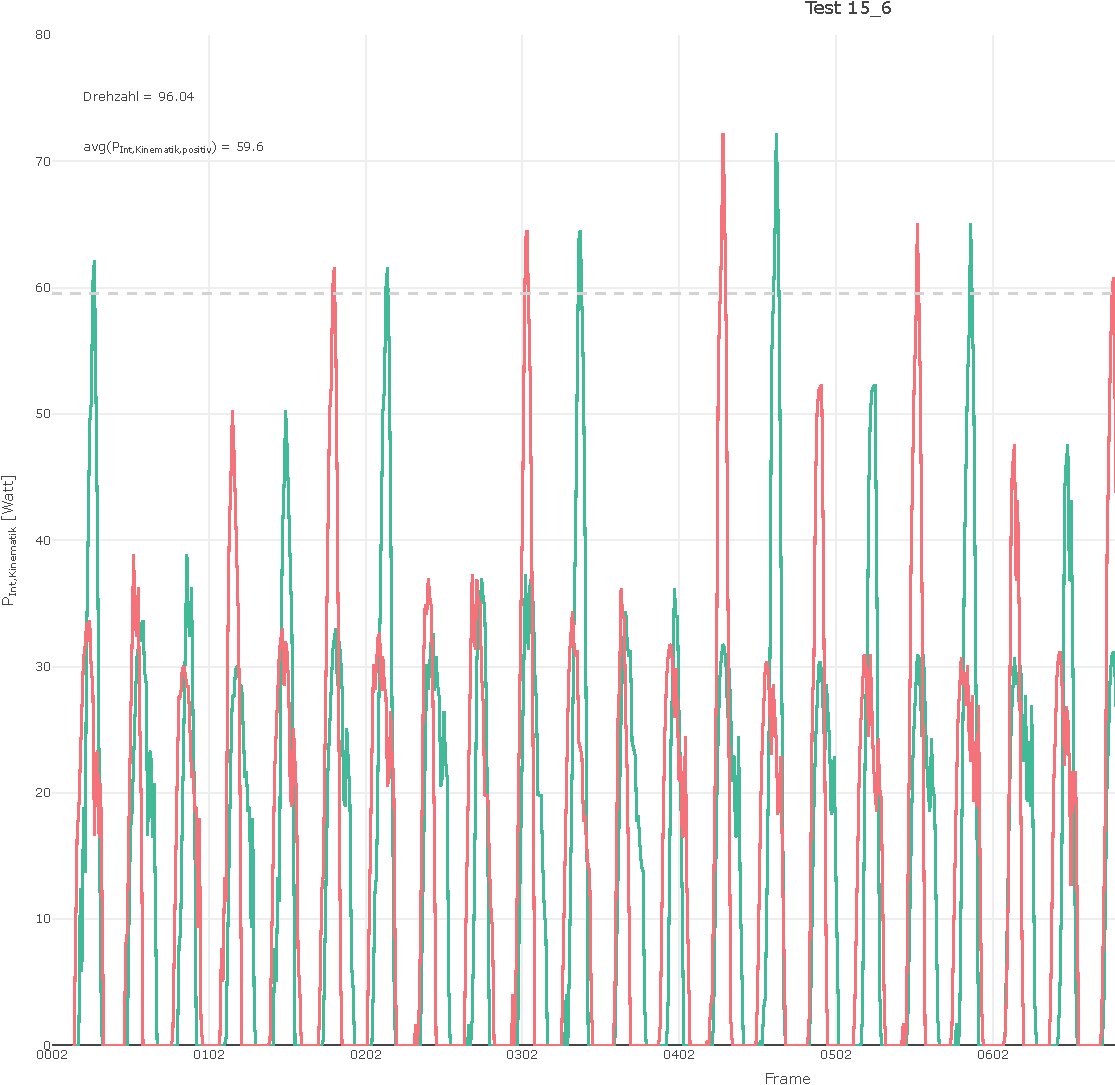
\includegraphics{Ergometer_Daten_files/figure-pdf/fig-PInt_Kinematik_15_6-1.pdf}

}

\caption{\label{fig-PInt_Kinematik_15_6}Zeitlicher Verlauf der aus der
3D-Kinematik berechneten positiven Anteile der inneren Leistung
(P\textsubscript{int}) beider Beine mit gemitteltem
P\textsubscript{int}-Wert (grau gestrichelt) für 15\_6.}

\end{figure}%

\subsubsection{Proband 19}

\paragraph{Test 1}

\begin{figure}

\centering{

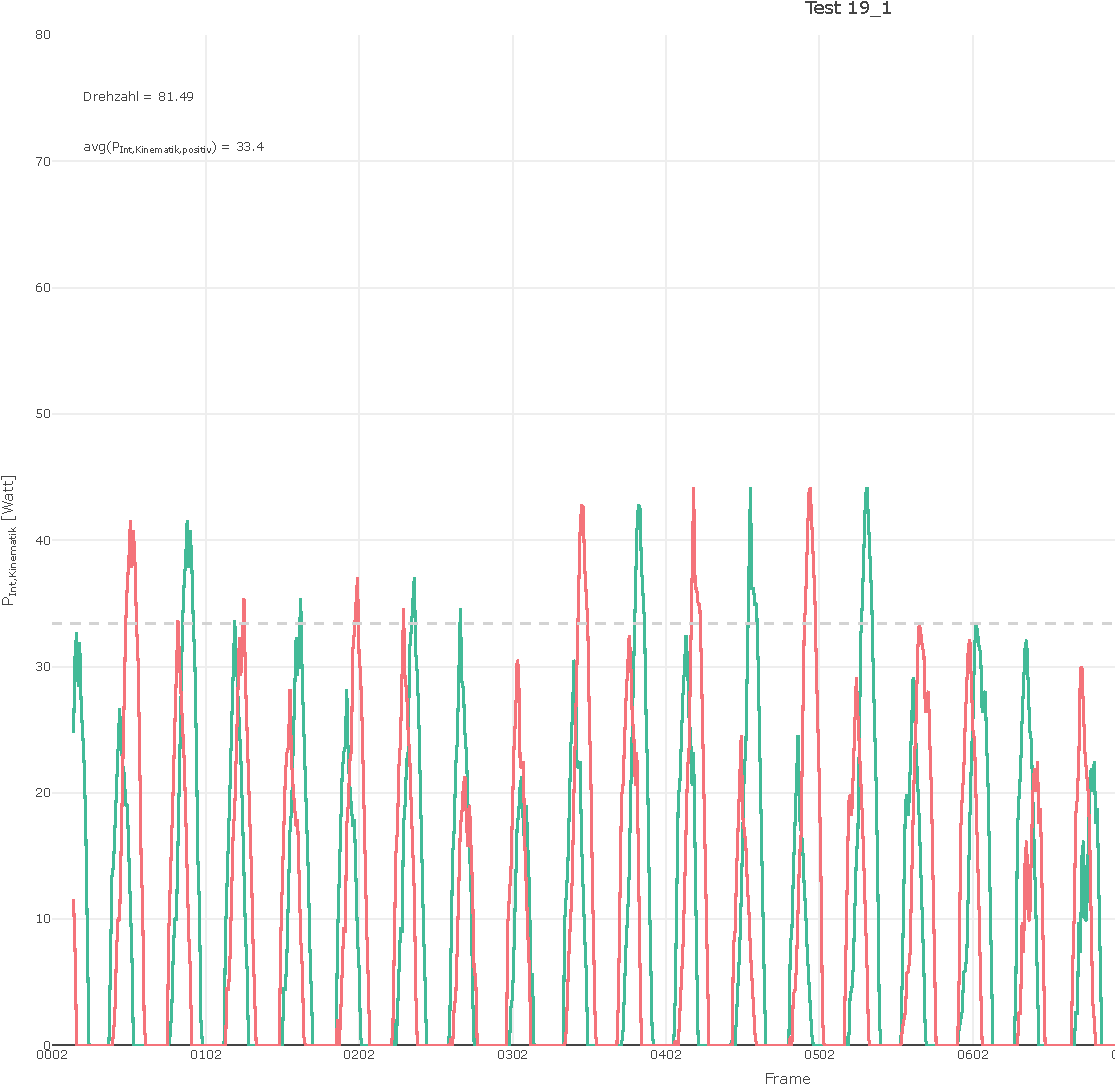
\includegraphics{Ergometer_Daten_files/figure-pdf/fig-PInt_Kinematik_19_1-1.pdf}

}

\caption{\label{fig-PInt_Kinematik_19_1}Zeitlicher Verlauf der aus der
3D-Kinematik berechneten positiven Anteile der inneren Leistung
(P\textsubscript{int}) beider Beine mit gemitteltem
P\textsubscript{int}-Wert (grau gestrichelt) für 19\_1.}

\end{figure}%

\paragraph{Test 2}

\begin{figure}

\centering{

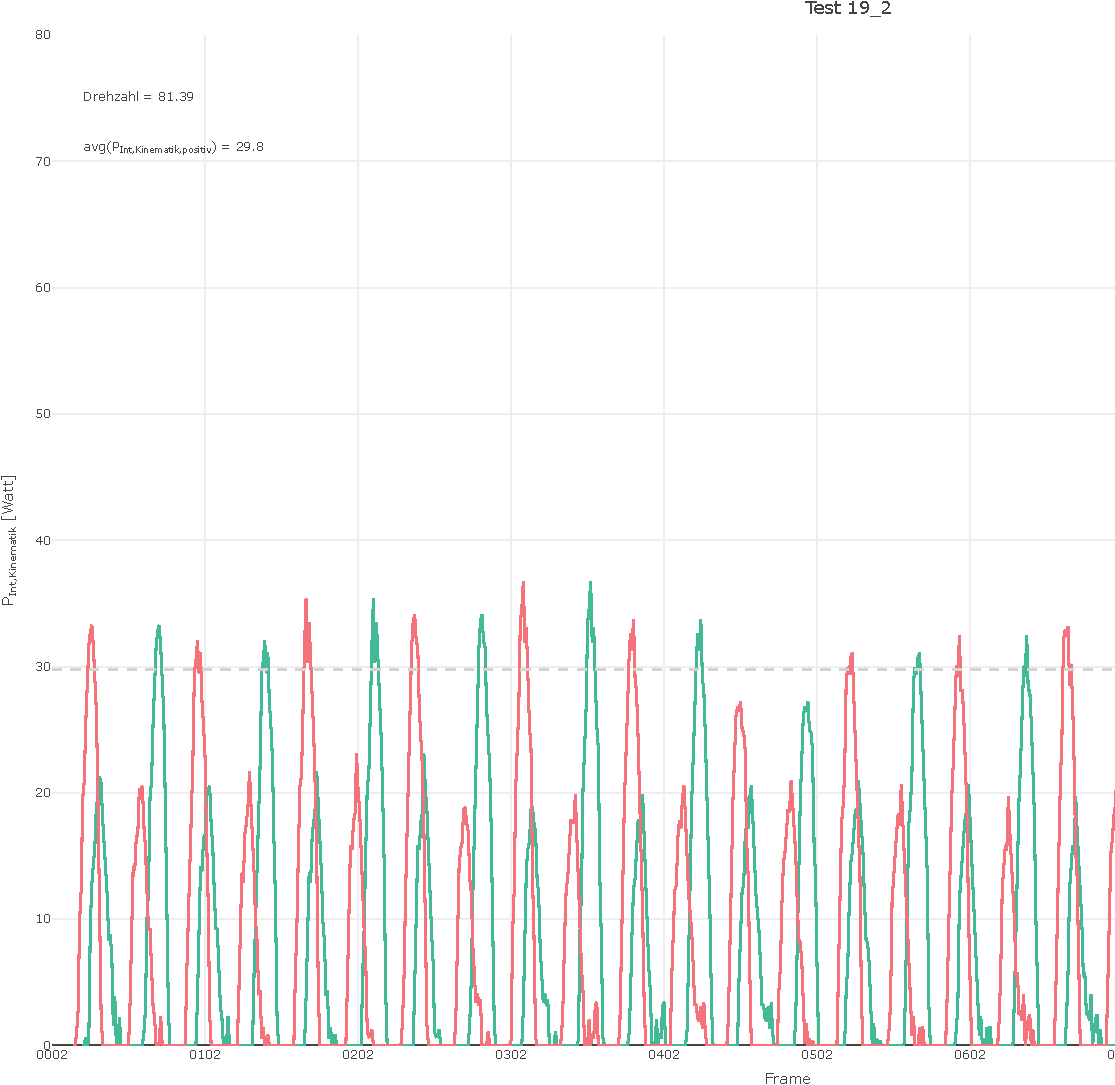
\includegraphics{Ergometer_Daten_files/figure-pdf/fig-PInt_Kinematik_19_2-1.pdf}

}

\caption{\label{fig-PInt_Kinematik_19_2}Zeitlicher Verlauf der aus der
3D-Kinematik berechneten positiven Anteile der inneren Leistung
(P\textsubscript{int}) beider Beine mit gemitteltem
P\textsubscript{int}-Wert (grau gestrichelt) für 19\_2.}

\end{figure}%

\paragraph{Test 3}

\begin{figure}

\centering{

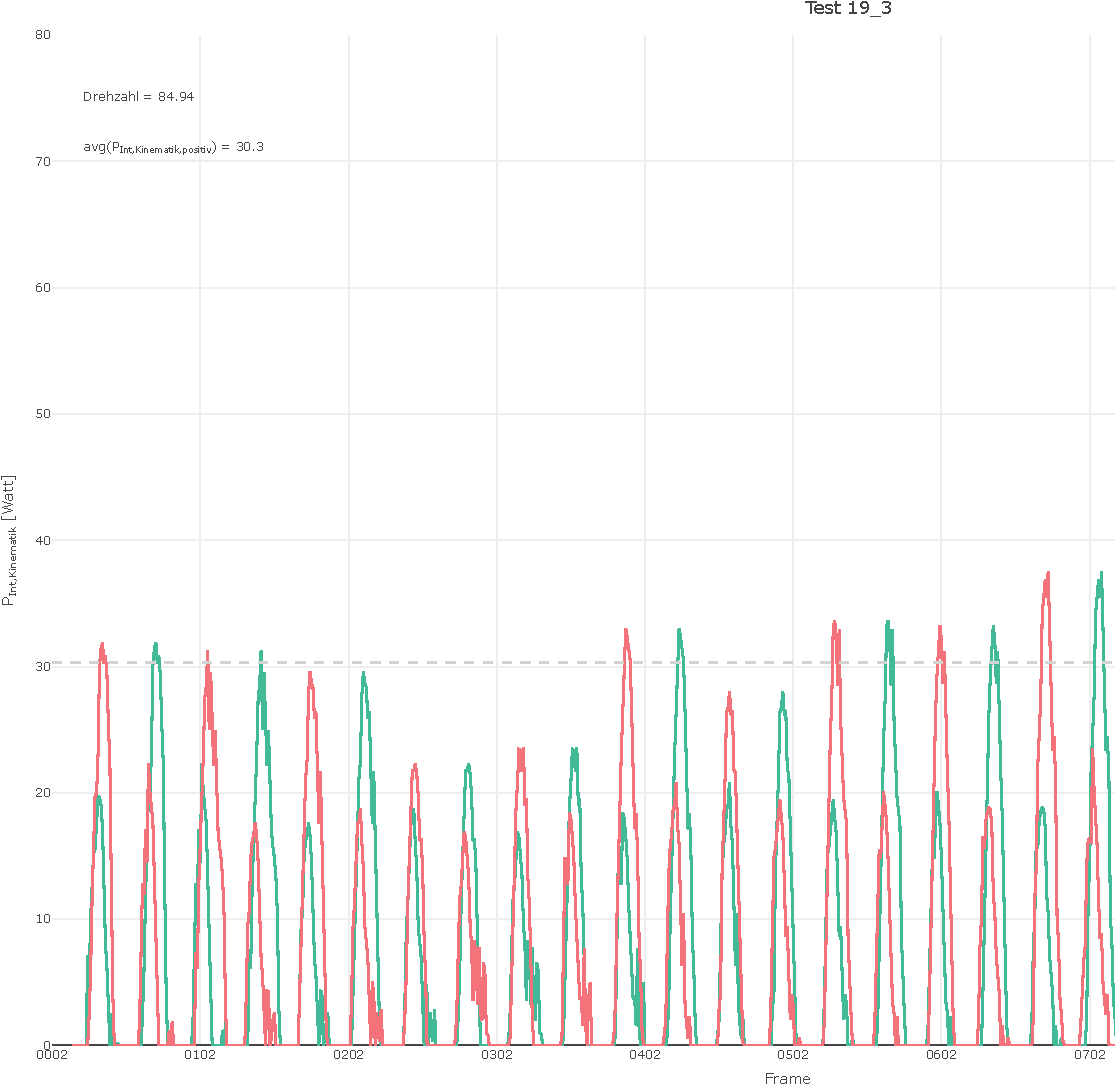
\includegraphics{Ergometer_Daten_files/figure-pdf/fig-PInt_Kinematik_19_3-1.pdf}

}

\caption{\label{fig-PInt_Kinematik_19_3}Zeitlicher Verlauf der aus der
3D-Kinematik berechneten positiven Anteile der inneren Leistung
(P\textsubscript{int}) beider Beine mit gemitteltem
P\textsubscript{int}-Wert (grau gestrichelt) für 19\_3.}

\end{figure}%

\paragraph{Test 4}

\begin{figure}

\centering{

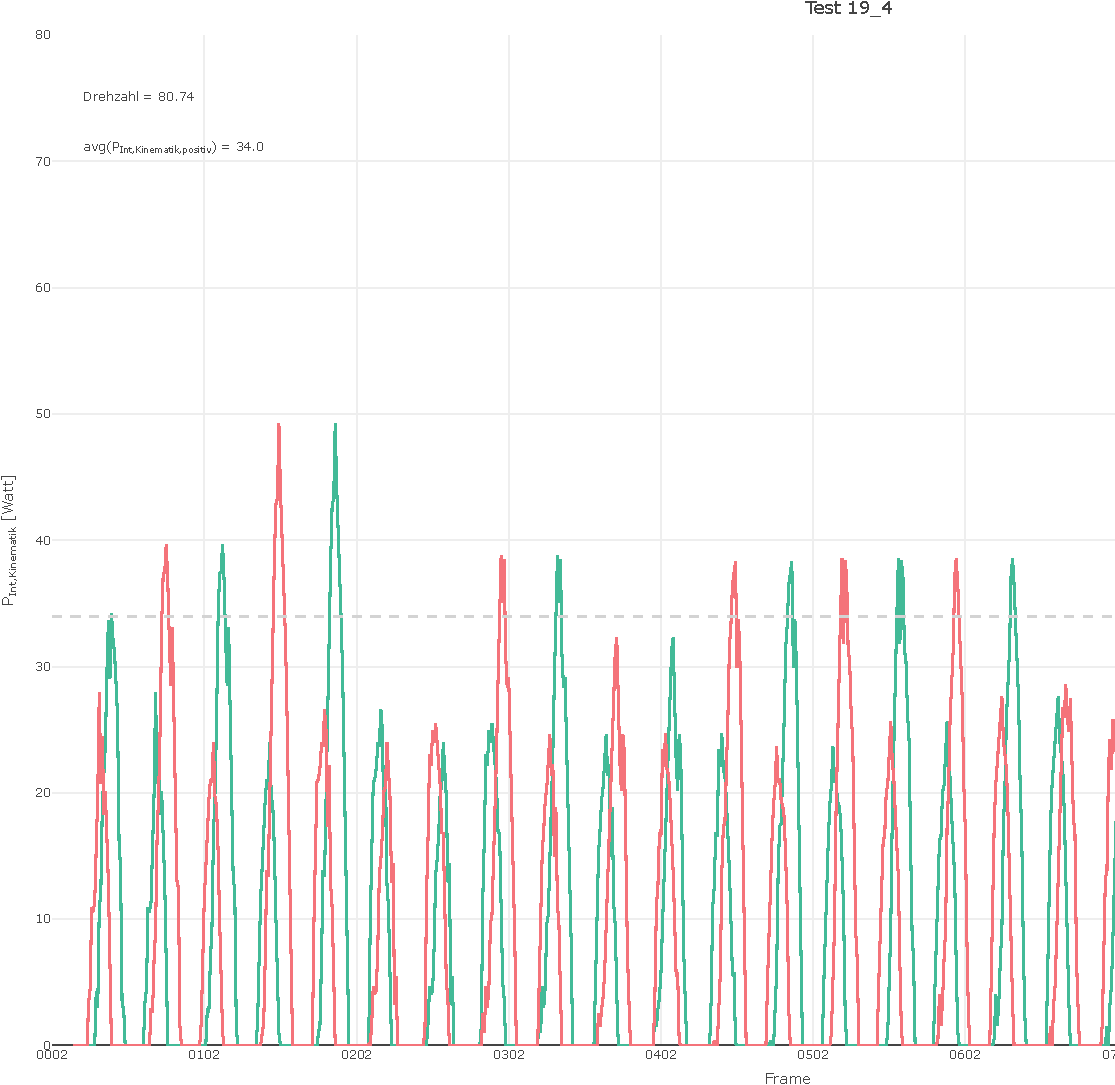
\includegraphics{Ergometer_Daten_files/figure-pdf/fig-PInt_Kinematik_19_4-1.pdf}

}

\caption{\label{fig-PInt_Kinematik_19_4}Zeitlicher Verlauf der aus der
3D-Kinematik berechneten positiven Anteile der inneren Leistung
(P\textsubscript{int}) beider Beine mit gemitteltem
P\textsubscript{int}-Wert (grau gestrichelt) für 19\_4.}

\end{figure}%

\paragraph{Test 5}

\begin{figure}

\centering{

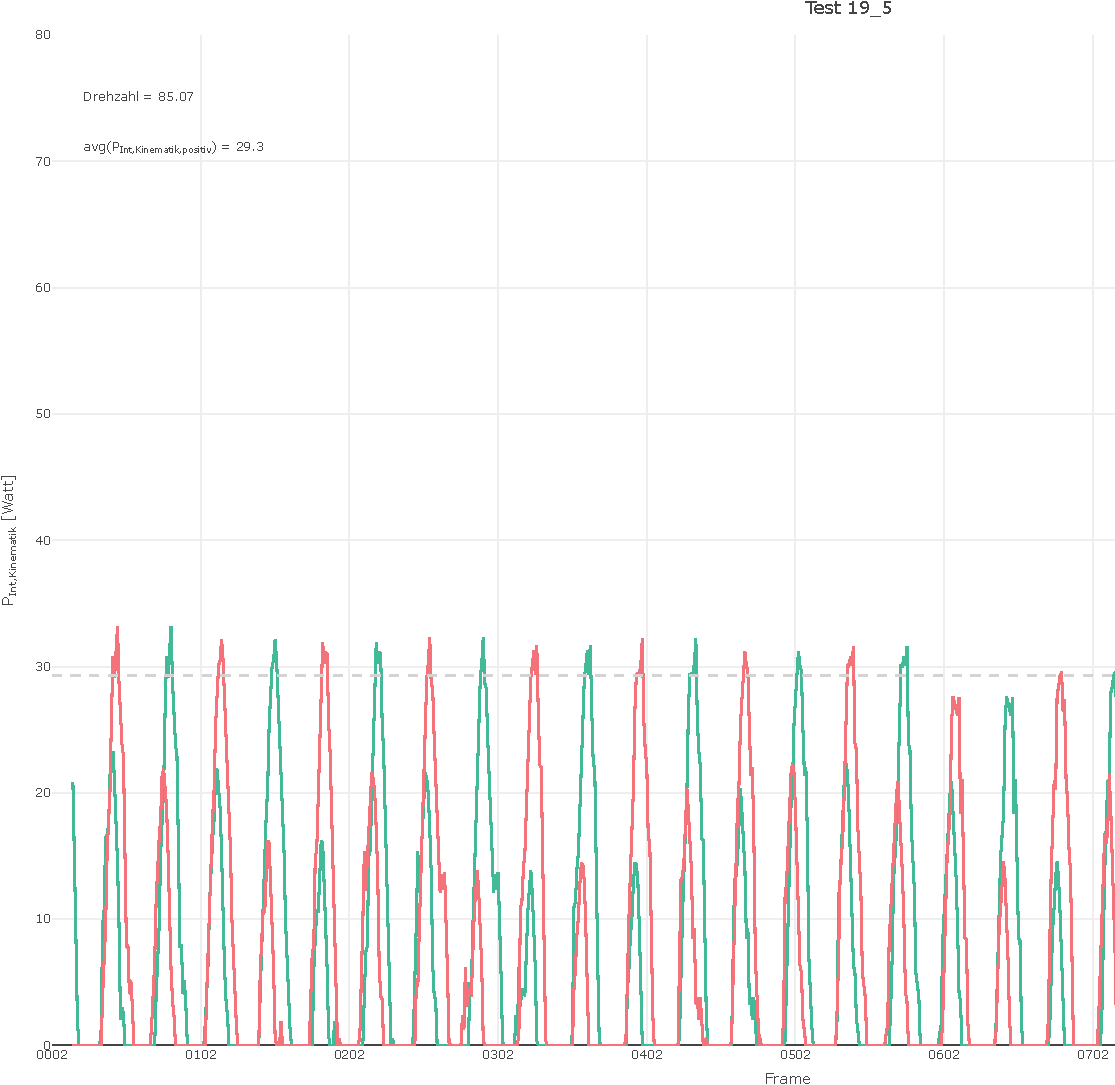
\includegraphics{Ergometer_Daten_files/figure-pdf/fig-PInt_Kinematik_19_5-1.pdf}

}

\caption{\label{fig-PInt_Kinematik_19_5}Zeitlicher Verlauf der aus der
3D-Kinematik berechneten positiven Anteile der inneren Leistung
(P\textsubscript{int}) beider Beine mit gemitteltem
P\textsubscript{int}-Wert (grau gestrichelt) für 19\_5.}

\end{figure}%

\paragraph{Test 6}

\begin{figure}

\centering{

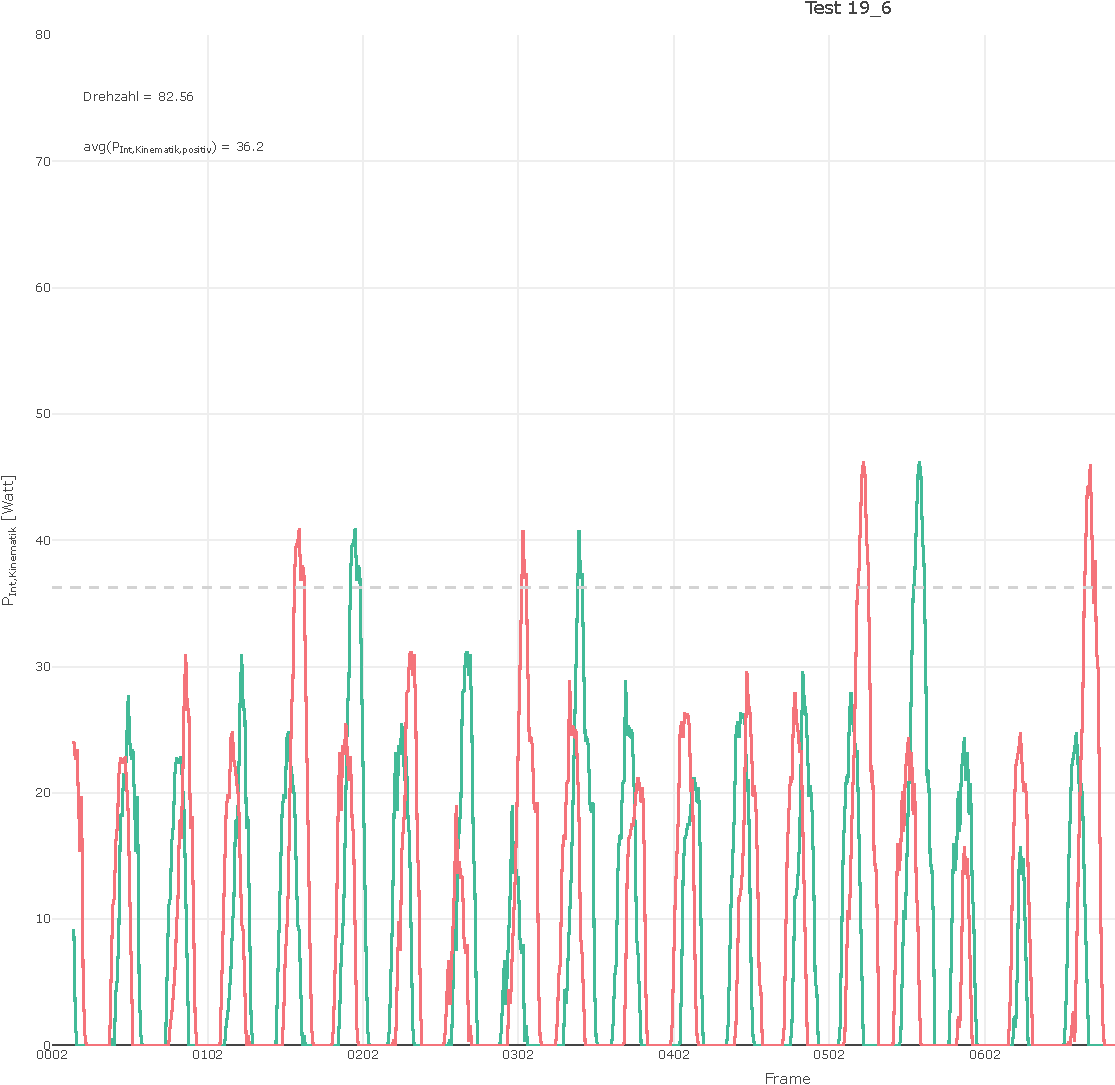
\includegraphics{Ergometer_Daten_files/figure-pdf/fig-PInt_Kinematik_19_6-1.pdf}

}

\caption{\label{fig-PInt_Kinematik_19_6}Zeitlicher Verlauf der aus der
3D-Kinematik berechneten positiven Anteile der inneren Leistung
(P\textsubscript{int}) beider Beine mit gemitteltem
P\textsubscript{int}-Wert (grau gestrichelt) für 19\_6.}

\end{figure}%

\subsubsection{Vergleich der berechneten inneren Leistungen:
Biomechanisches Modell, 3D-Kinematik und
Minetti-Berechnung}\label{vergleich-der-berechneten-inneren-leistungen-biomechanisches-modell-3d-kinematik-und-minetti-berechnung}

Abbildung~\ref{fig-Vergleich_PInt_Kin_Mod} zeigt einen direkten
Vergleich der inneren Leistung (P\textsubscript{Int}), die mittels drei
verschiedener Methoden (Biomechanisches Modell, 3D-Kinematik und
Minetti-Berechnung) für verschiedene Probanden ermittelt wurde. Im
niedrigen Drehzahlbereich (60-70 min\textsuperscript{-1}) zeigen alle
drei Berechnungsmethoden noch relativ ähnliche Werte mit
P\textsubscript{Int} zwischen 10 und 25 Watt. Mit steigender Drehzahl
wird eine zunehmende Abweichung zwischen den Methoden erkennbar. Die
Minetti-Berechnung (Dreiecke) tendiert dabei zu den höchsten Werten,
während das biomechanische Modell (Kreise) meist die niedrigsten Werte
liefert. Die aus der 3D-Kinematik ermittelten Werte (Quadrate)
positionieren sich in der Regel zwischen diesen beiden Extremen. Bei
Drehzahlen oberhalb von 85 min\textsuperscript{-1} zeigt sich sich eine
progressive Abweichung zwischen der Minetti-Berechnung und den anderen
beiden Methoden.

\begin{figure}

\centering{

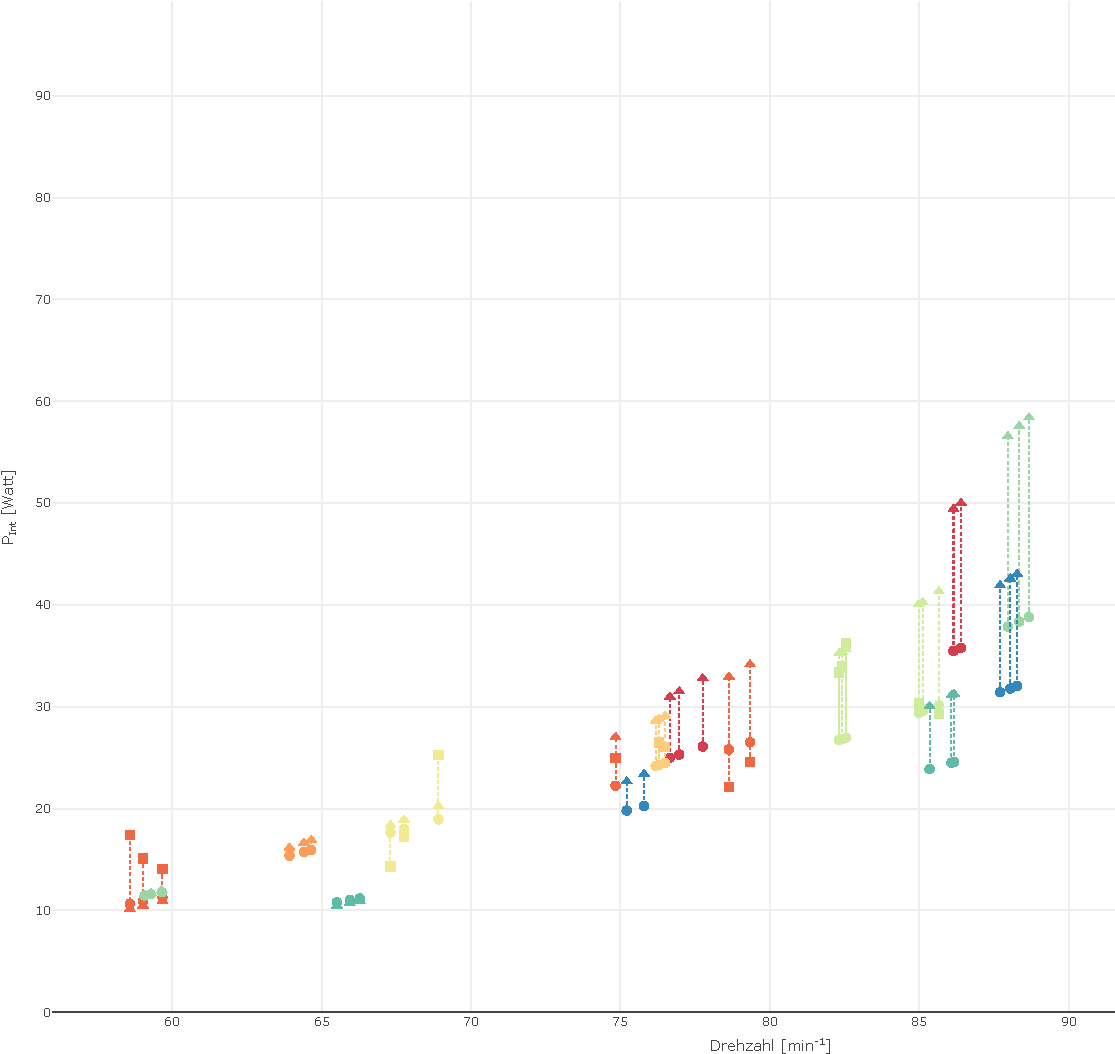
\includegraphics{Ergometer_Daten_files/figure-pdf/fig-Vergleich_PInt_Kin_Mod-1.pdf}

}

\caption{\label{fig-Vergleich_PInt_Kin_Mod}Vergleich der berechneten
inneren Leistungen: Biomechanisches Modell, 3D-Kinematik und
Minetti-Berechnung}

\end{figure}%

\subsubsection{Individuelle Darstellung und kubische Modellierung der
inneren Leistung aus dem biomechanischen Modell, der 3D-Kinematik und
der kombinierten
Berechnung}\label{individuelle-darstellung-und-kubische-modellierung-der-inneren-leistung-aus-dem-biomechanischen-modell-der-3d-kinematik-und-der-kombinierten-berechnung}

Die Abbildungen Abbildung~\ref{fig-PInt_Mod},
Abbildung~\ref{fig-PInt_Kin} und Abbildung~\ref{fig-PInt_Kin_Mod}
illustrieren die körpergewichtsbezogene innere Leistung in Relation zur
Trittrate, wobei jeweils eine kubische Modellfunktion den Verlauf der
jeweiligen P\textsubscript{Int}-Berechnung für die steigenden Drehzahlen
beschreibt. Das biomechanische Modell (Abbildung~\ref{fig-PInt_Mod})
liefert dabei eine vollständige Datenbasis für alle Probanden und
Belastungen mit einer sehr guten Modellanpassung (R² = 0.999, y =
0.00000075x³). Die kinematikbasierte Analyse
(Abbildung~\ref{fig-PInt_Kin}) beschränkt sich auf die
Belastungsintensitäten mit verfügbaren 3D-Kinematik Daten, zeigt jedoch
einen vergleichbaren Funktionsverlauf (R² = 0.983, y = 0.00000077x³).
Die Kombination beider Methoden (Abbildung~\ref{fig-PInt_Kin_Mod})
ermöglicht durch Einbeziehung der mittleren Differenzen zwischen
kinematischer und modellierter innerer Leistung eine Approximation für
Belastungsintensitäten ohne Kinematikdaten. Die konsistente
Charakteristik der kubischen Modellfunktionen über alle drei
Berechnungsansätze unterstützt die gewählte mathematische Beschreibung
des Zusammenhangs zwischen Trittrate und innerer Leistung.

\paragraph{\texorpdfstring{P\textsubscript{Int,Modell}}{PInt,Modell}}

\begin{figure}

\centering{

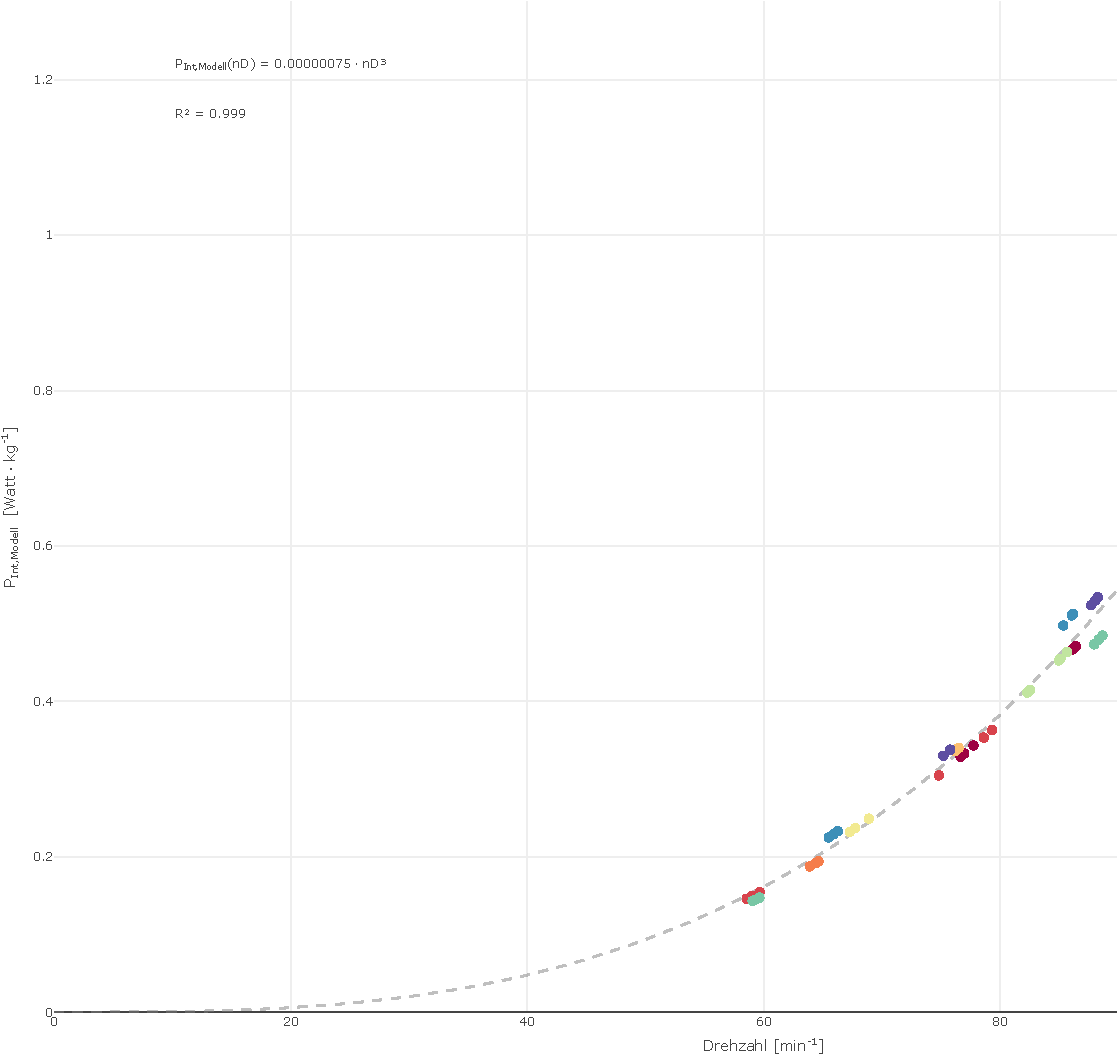
\includegraphics{Ergometer_Daten_files/figure-pdf/fig-PInt_Mod-1.pdf}

}

\caption{\label{fig-PInt_Mod}Körpergewichtsbezogene innere Leistung von
P\textsubscript{Int,Modell} in Abhängigkeit von der Trittrate mit
kubischer Modellfunktion (y = 0.00000075x³, R² = 0.999).}

\end{figure}%

\paragraph{\texorpdfstring{P\textsubscript{Int,Kinematik}}{PInt,Kinematik}}

\begin{figure}

\centering{

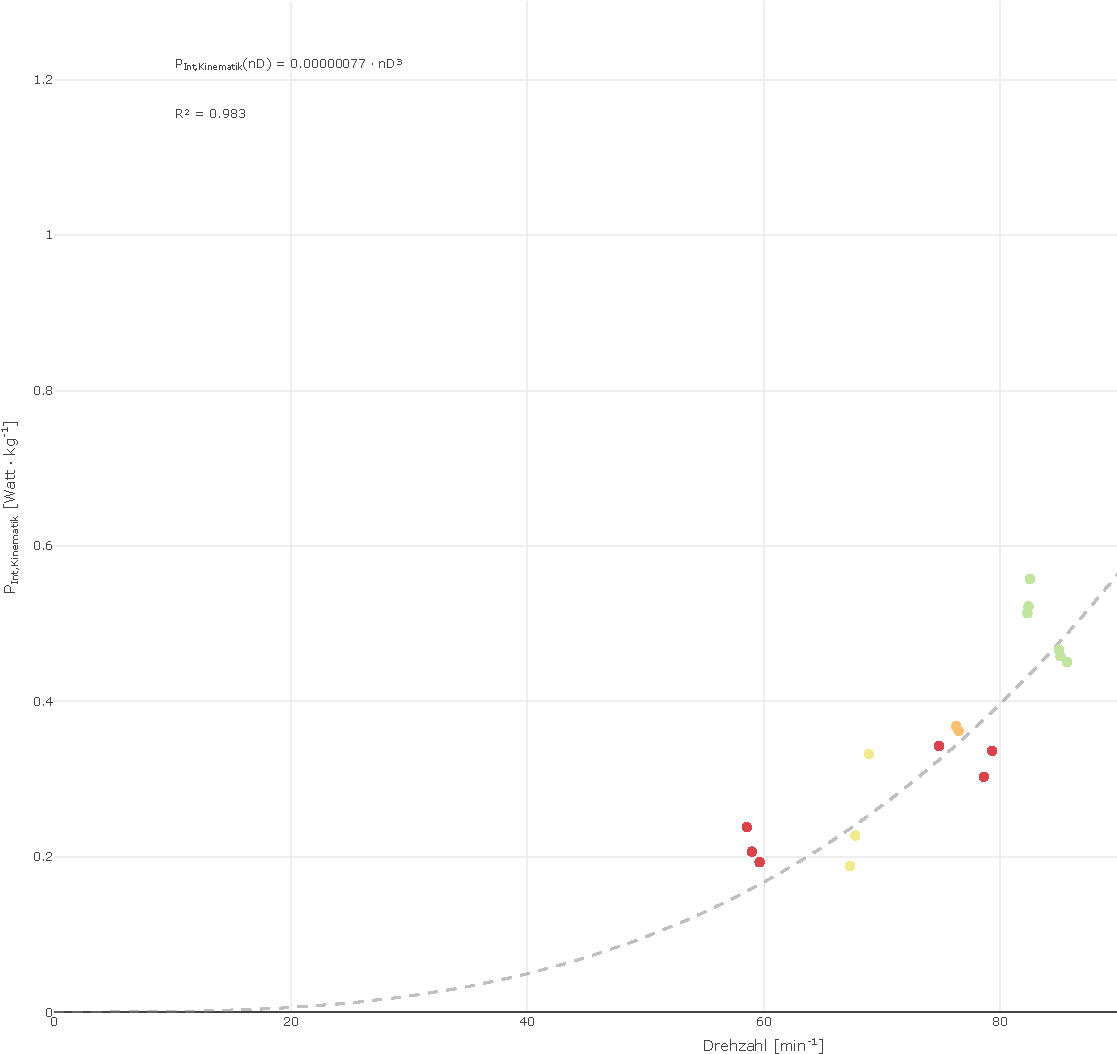
\includegraphics{Ergometer_Daten_files/figure-pdf/fig-PInt_Kin-1.pdf}

}

\caption{\label{fig-PInt_Kin}Körpergewichtsbezogene innere Leistung von
P\textsubscript{Int,Kinematik} in Abhängigkeit von der Trittrate mit
kubischer Modellfunktion (y = 0.00000077x³, R² = 0.983).}

\end{figure}%

\paragraph{\texorpdfstring{P\textsubscript{Int,Kinematik,Modell}}{PInt,Kinematik,Modell}}

\begin{figure}

\centering{

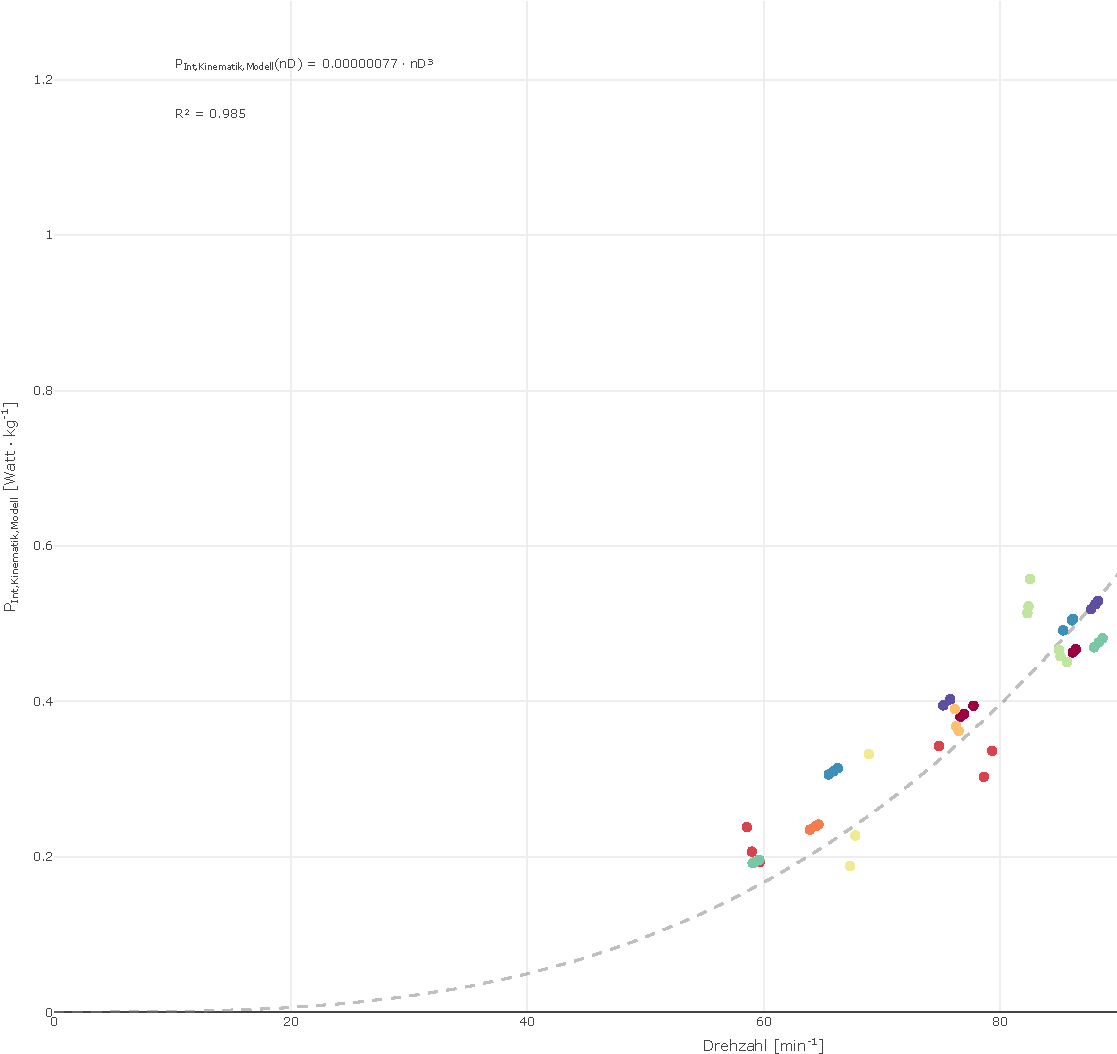
\includegraphics{Ergometer_Daten_files/figure-pdf/fig-PInt_Kin_Mod-1.pdf}

}

\caption{\label{fig-PInt_Kin_Mod}Körpergewichtsbezogene innere Leistung
von P\textsubscript{Int,Kinematik,Modell} in Abhängigkeit von der
Trittrate mit kubischer Modellfunktion (y = 0.00000077x³, R² = 0.985).}

\end{figure}%

\subsubsection{Modellvergleich: Einfluss von Körpermasse und Drehzahl
auf die innere
Leistung}\label{modellvergleich-einfluss-von-kuxf6rpermasse-und-drehzahl-auf-die-innere-leistung}

Die nachfolgenden Abbildungen zeigen die berechnete innere Leistung
(P\textsubscript{Int}) in Abhängigkeit von Drehzahl und Körpermasse auf
Basis des biomechanischen Modells (Abbildung~\ref{fig-PInt_Modell}) und
die Berechnung nach Minetti et al. (2001)
(Abbildung~\ref{fig-PInt_Minetti}). Beide Berechnungsmethoden weisen
eine nicht-lineare Charakteristik der P\textsubscript{Int} auf, die
sowohl mit steigender Drehzahl als auch mit zunehmender Körpermasse
progressiv ansteigt. Diese Systematik manifestiert sich in einer
systematisch gestaffelten Verteilung der Kurvenverläufe entsprechend der
verschiedenen Körpermassen. Für einen exemplarischen Vergleich bei 70 kg
Körpermasse ergeben sich die P\textsubscript{Int}-Werte der
Tabelle~\ref{tbl-PInt_Vergleich}. Die Tabelle enthält neben den zwei
berechneten P\textsubscript{Int}-Werten auch die während des
Drehzahltests ermittelten Werte des Sauerstoffumsatzes für die
Leerbewegung (O\textsubscript{2}-Cost\textsubscript{nD}). Diese wurden
mittels der kubischen Modellfunktion
\(\dot{V}\mathrm{O}_{2,\text{net}}(\text{nD}) \ [\text{ml} \cdot \text{min}^{-1} \cdot \text{kg}^{-1}] = 0.000011 \cdot \text{nD}^3\)
berechnet. Für die Umrechnung der
O\textsubscript{2}-Cost\textsubscript{nD}-Werte in die korrespondierende
mechanische Leistung {[}W{]} wurde ein konservativer
O\textsubscript{2}-Leistungs-Äquivalent von 10
ml·min\textsuperscript{-1} · W\textsuperscript{-1} gewählt. Dieser
Umrechnungsfaktor orientiert sich an den in der Literatur dokumentierten
Werten, die typischerweise im Bereich von 8.5-12.0
ml·min\textsuperscript{-1} · W\textsuperscript{-1} liegen (Hansen et
al., 1984; Heck et al., 2022; Özyener et al., 2001; Rassouli \&
Thurnheer, 2015; Wasserman et al., 2011).

\begin{longtable}[]{@{}
  >{\raggedright\arraybackslash}p{(\columnwidth - 6\tabcolsep) * \real{0.2316}}
  >{\raggedright\arraybackslash}p{(\columnwidth - 6\tabcolsep) * \real{0.2000}}
  >{\raggedright\arraybackslash}p{(\columnwidth - 6\tabcolsep) * \real{0.2000}}
  >{\raggedright\arraybackslash}p{(\columnwidth - 6\tabcolsep) * \real{0.3684}}@{}}
\caption{Vergleich der P\textsubscript{Int,Modell} und
P\textsubscript{Int,Minetti} für ausgewählte
Drehzahlen.}\label{tbl-PInt_Vergleich}\tabularnewline
\toprule\noalign{}
\begin{minipage}[b]{\linewidth}\raggedright
Drehzahl {[}U·min\textsuperscript{-1}{]}
\end{minipage} & \begin{minipage}[b]{\linewidth}\raggedright
P\textsubscript{Int,Modell} {[}W{]}
\end{minipage} & \begin{minipage}[b]{\linewidth}\raggedright
P\textsubscript{Int,Minetti} {[}W{]}
\end{minipage} & \begin{minipage}[b]{\linewidth}\raggedright
O\textsubscript{2}-Cost\textsubscript{nD}
{[}ml·min\textsuperscript{-1}{]}
\end{minipage} \\
\midrule\noalign{}
\endfirsthead
\toprule\noalign{}
\begin{minipage}[b]{\linewidth}\raggedright
Drehzahl {[}U·min\textsuperscript{-1}{]}
\end{minipage} & \begin{minipage}[b]{\linewidth}\raggedright
P\textsubscript{Int,Modell} {[}W{]}
\end{minipage} & \begin{minipage}[b]{\linewidth}\raggedright
P\textsubscript{Int,Minetti} {[}W{]}
\end{minipage} & \begin{minipage}[b]{\linewidth}\raggedright
O\textsubscript{2}-Cost\textsubscript{nD}
{[}ml·min\textsuperscript{-1}{]}
\end{minipage} \\
\midrule\noalign{}
\endhead
\bottomrule\noalign{}
\endlastfoot
60 & 13.4 & 10.71 & 166.3 ≙ 16.6 {[}W{]} \\
80 & 31.7 & 33.8 & 394.2 ≙ 39.4 {[}W{]} \\
100 & 62.0 & 82.6 & 770.0 ≙ 77.0 {[}W{]} \\
120 & 107.1 & 171.4 & 1330.6 ≙ 133.1 {[}W{]} \\
150 & 209.1 & 418.4 & 2598.8 ≙ 259.9 {[}W{]} \\
200 & 495.6 & 1322.2 & 6160.0 ≙ 616.0 {[}W{]} \\
\end{longtable}

Während das biomechanische Modell initial einen vergleichbaren Anstieg
aufweist, zeigt die Minetti-Berechnung insbesondere bei Trittraten
oberhalb von 150 U ⋅ min\textsuperscript{-1} einen deutlich stärkeren
Anstieg. Diese abweichenden Charakteristika in den Anstiegen resultieren
speziell im hohen Drehzahlbereich in deutlichen Differenzen der
absoluten Leistungswerte, wobei die Minetti-Berechnung bei einer
Trittrate von 200 U ⋅ min\textsuperscript{-1} nahezu das Dreifache der
modellierten Werte erreicht. Die metabolischen
O\textsubscript{2}-Cost\textsubscript{nD}-Werte liegen bei Drehzahlen
bis etwa 100 U·min\^{}\{-1\} über beiden theoretischen Berechnungen und
bewegen sich bei höheren Drehzahlen zwischen den Werten der beiden
Modellansätze.

\subsubsection{\texorpdfstring{P\textsubscript{Int,Modell}}{PInt,Modell}}

\begin{figure}

\centering{

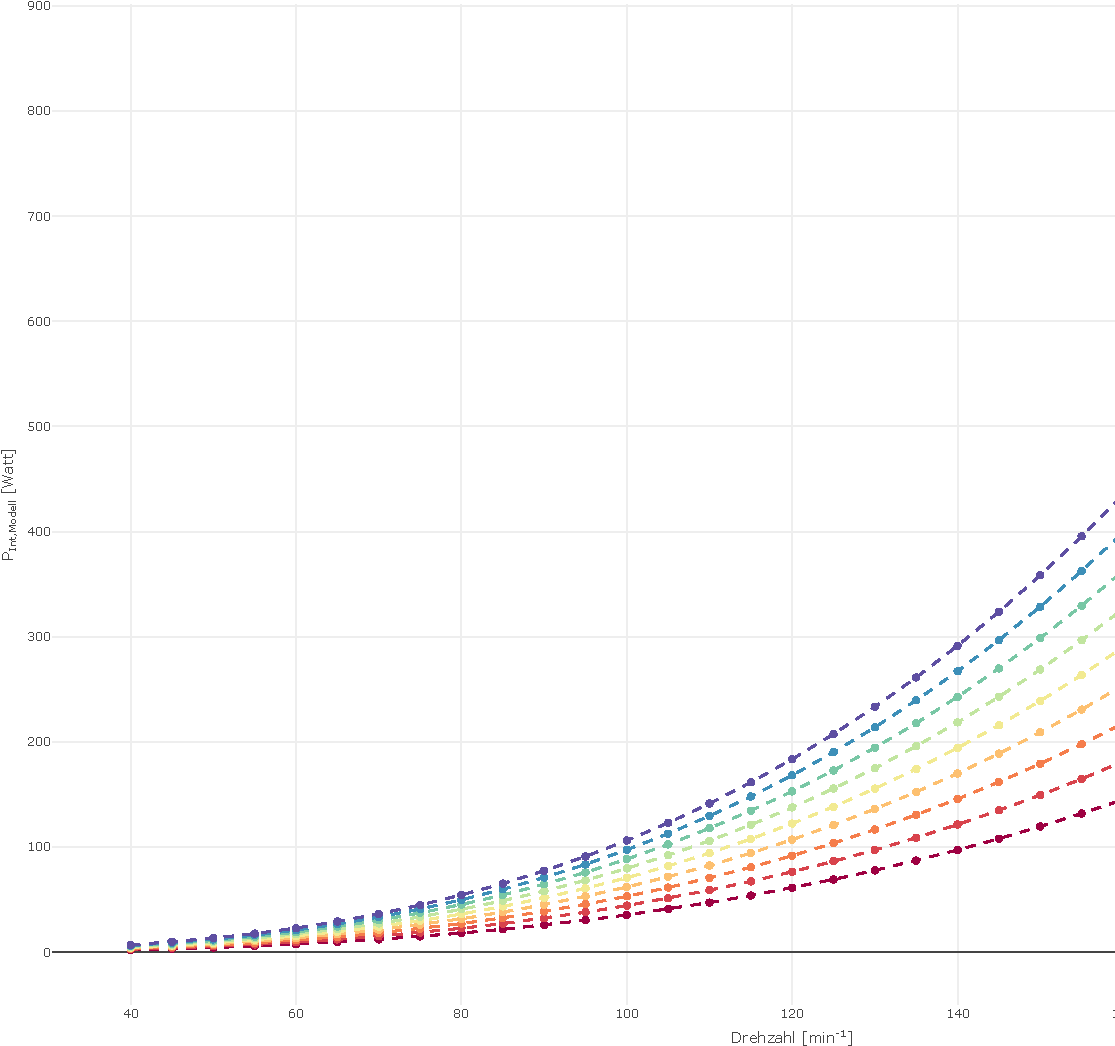
\includegraphics{Ergometer_Daten_files/figure-pdf/fig-PInt_Modell-1.pdf}

}

\caption{\label{fig-PInt_Modell}PInt,Modell für verschiedene
Körpermassen und Drehzahlen bei den mittleren anthropometrischen
Modellparametern aller Probanden (Oberschenkellänge: 41,7 cm,
Unterschenkellänge: 55,2 cm, Beinlänge: 122,9 cm, Oberschenkelumfang:
57,2 cm, Unterschenkelumfang: 36,2 cm) und einer theoretischen
Kurbellänge von 17,3 cm.}

\end{figure}%

\subsubsection{\texorpdfstring{P\textsubscript{Int,Minetti}}{PInt,Minetti}}

\begin{figure}

\centering{

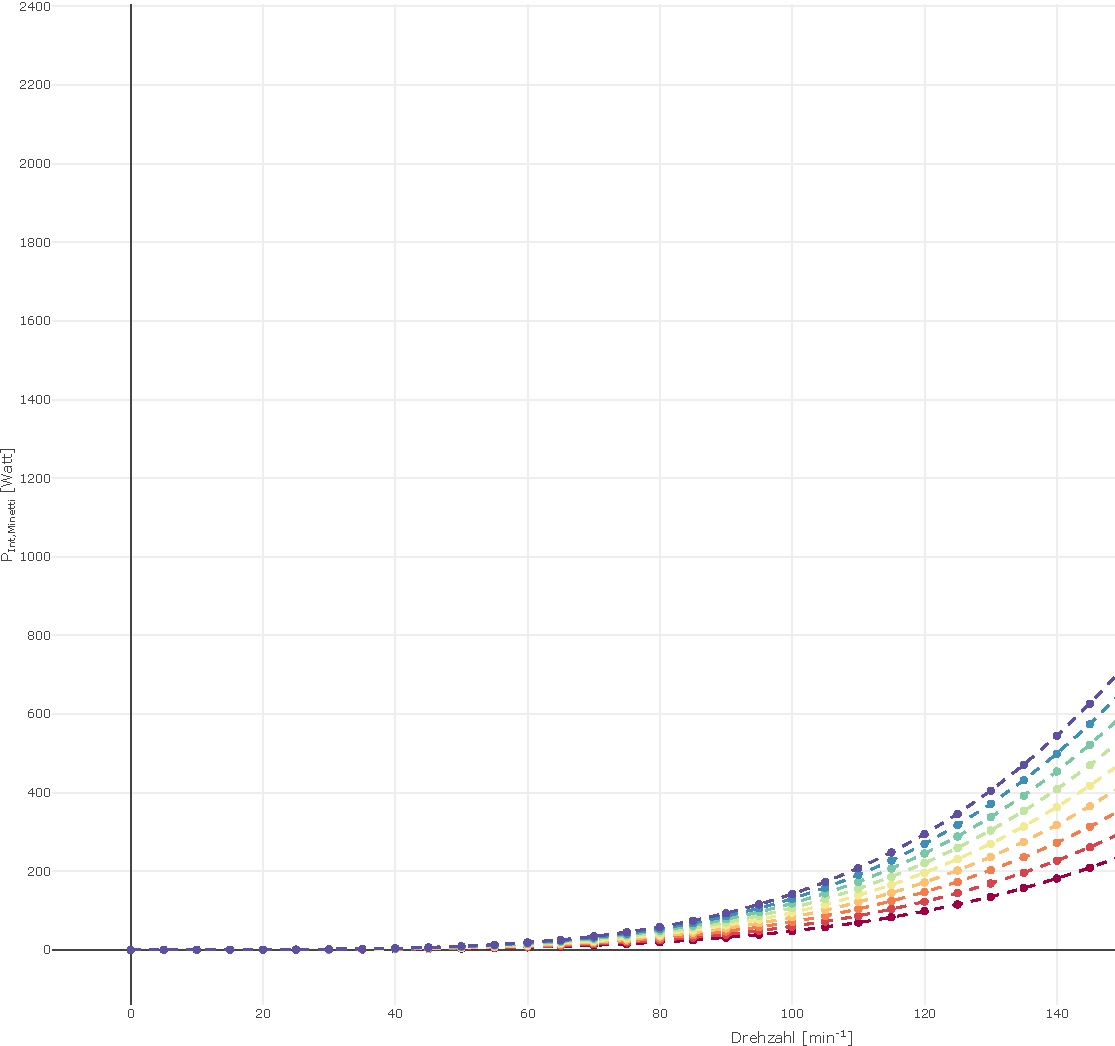
\includegraphics{Ergometer_Daten_files/figure-pdf/fig-PInt_Minetti-1.pdf}

}

\caption{\label{fig-PInt_Minetti}PInt,Minetti für verschiedene
Körpermassen und Drehzahlen}

\end{figure}%

\section{Quellenverzeichnis}\label{quellenverzeichnis}

\phantomsection\label{refs}
\begin{CSLReferences}{1}{0}
\bibitem[\citeproctext]{ref-Hansen1984}
Hansen, J. E., Sue, D. Y., \& Wasserman, K. (1984). {Predicted values
for clinical exercise testing}. \emph{American Review of Respiratory
Disease}, \emph{129}(2 SUPPL.).
\url{https://doi.org/10.1164/arrd.1984.129.2p2.s49}

\bibitem[\citeproctext]{ref-Heck2022}
Heck, H., Bartmus, U., \& Grabow, V. (2022). \emph{{Laktat}} (1. Aufl.,
S. 662). Springer Berlin Heidelberg.

\bibitem[\citeproctext]{ref-Minetti2001}
Minetti, A. E., Pinkerton, J., \& Zamparo, P. (2001). {From bipedalism
to bicyclism: evolution in energetics and biomechanics of historic
bicycles.} \emph{Proceedings. Biological sciences}, \emph{268}(1474),
1351--1360. \url{https://doi.org/10.1098/rspb.2001.1662}

\bibitem[\citeproctext]{ref-Oezyener2001}
Özyener, F., Rossiter, H. B., Ward, S. A., \& Whipp, B. J. (2001).
{Influence of exercise intensity on the on- and off-transient kinetics
of pulmonary oxygen uptake in humans.} \emph{The Journal of physiology},
\emph{533}(Pt 3), 891--902.
\url{https://doi.org/10.1111/j.1469-7793.2001.t01-1-00891.x}

\bibitem[\citeproctext]{ref-Rassouli2015}
Rassouli, F., \& Thurnheer, R. (2015). {Spiroergometrie -- Indikation,
Durchf{ü}hrung und Interpretation}. \emph{Swiss Medical Forum ‒
Schweizerisches Medizin-Forum}, \emph{15}(1415), 315--321.
\url{https://doi.org/10.4414/smf.2015.02227}

\bibitem[\citeproctext]{ref-Wasserman2011}
Wasserman, K., Hansen, J. E., Sue, D. Y., Stringer, W. W., Sietsema, K.
E., Sun, X. G., \& Whipp, B. J. (2011). \emph{{Principles of exercise
testing and interpretation: Including pathophysiology and clinical
applications: Fifth edition}} (S. 1--592).
\url{https://doi.org/10.1097/00024382-200014010-00017}

\end{CSLReferences}



\end{document}
